%%%%%%%%%%%%%%%%%%%%%%%%%%%%%%%%%%%%%%%%%%%%%%%%%%%
%% LaTeX book template                           %%
%% Author:  Amber Jain (http://amberj.devio.us/) %%
%% License: ISC license                          %%
%%%%%%%%%%%%%%%%%%%%%%%%%%%%%%%%%%%%%%%%%%%%%%%%%%%
%!TEX TS-program = pdfLaTeX
%!TEX encoding = utf-8
%!TEX spellcheck = fr-FR

\documentclass[12pt,twoside,openright]{book}

%\usepackage{soul}

%\documentclass[a4paper,11pt]{book}
\usepackage[T1]{fontenc}
\usepackage[utf8]{inputenc}
\usepackage[francais]{babel}

\usepackage[usenames,dvipsnames]{color}

\usepackage{lmodern}
%%%%%%%%%%%%%%%%%%%%%%%%%%%%%%%%%%%%%%%%%%%%%%%%%%%%%%%%%
% Source: http://en.wikibooks.org/wiki/LaTeX/Hyperlinks %
%%%%%%%%%%%%%%%%%%%%%%%%%%%%%%%%%%%%%%%%%%%%%%%%%%%%%%%%%
\usepackage{hyperref}
\usepackage{graphicx}
\usepackage{pdfpages}
\usepackage{amsmath}
\usepackage{amssymb}
\usepackage{a4}
\usepackage{indentfirst}
\usepackage{fancyhdr}
\usepackage{varioref}
\usepackage{makeidx}

\usepackage{mslapa}

\usepackage{ulem}

%\usepackage{apacite}
%\usepackage[longnamesfirst,nonamebreak]{natbib}




%%%%%%%%%%%%%%%%%%%%%%%%%%%%%%%%%%%%%%%%%%%%%%%%%%%%%%%%%%%%%%%%%%%%%%%%%%%%%%
%%%%%%%%%%%%%%%%%%%%%%%%%%%%%%%%%%%%%%%%%%%%%%%%%%%%%%%%%%%%%%%%%%%%%%%%%%%%%%

\pagestyle{fancy}

\addtolength{\headwidth}{\marginparsep}
\addtolength{\headwidth}{\marginparwidth}
\renewcommand{\chaptermark}[1]{\markboth{#1}{}}
\renewcommand{\sectionmark}[1]{\markright{\thesection\ #1}}
\fancyhf{}
\fancyhead[LE,RO]{\bfseries\thepage}
\fancyhead[LO]{\bfseries\rightmark}
\fancyhead[RE]{\bfseries\leftmark}
\fancypagestyle{plain}{
\fancyhead{} % get rid of headers
\renewcommand{\headrulewidth}{0pt} % and the line
}


%% Apalike hyphenation %%%
%\let\oldbibitem=\bibitem
%\renewcommand{\bibitem}[2][]{\oldbibitem[#1]{#2}\newline}

%%% Margins %%%
\voffset -1.04cm
\textheight 23cm
\hoffset -1in
\evensidemargin 2.5cm
\oddsidemargin 2.5cm
\textwidth 16cm

%%%%%%%%%%%%%%%%%%%%%%%%%%%%%%%%%%%%%%%%%%%%%%%%%%%%%%%%%%%%%%%%%%%%%%%%%%%%%%
%%%%%%%%%%%%%%%%%%%%%%%%%%%%%%%%%%%%%%%%%%%%%%%%%%%%%%%%%%%%%%%%%%%%%%%%%%%%%%

%\textwidth16cm
%\textheight23cm
%\oddsidemargin0,5cm
%\evensidemargin0,5cm
%\topmargin-1cm
%\parskip0,5cm
%\parindent0cm



%%%%%%%%%%%%%%%%%%%%%%%%%%%%%%%%%%%%%%%%%%%%%%%%%%%%%%%%%%%%%%%%%%%%%%%%%%%%%%%%
% 'dedication' environment: To add a dedication paragraph at the start of book %
% Source: http://www.tug.org/pipermail/texhax/2010-June/015184.html            %
%%%%%%%%%%%%%%%%%%%%%%%%%%%%%%%%%%%%%%%%%%%%%%%%%%%%%%%%%%%%%%%%%%%%%%%%%%%%%%%%
\newenvironment{dedication}
{
   \cleardoublepage
   \thispagestyle{empty}
   \vspace*{\stretch{1}}
   \hfill\begin{minipage}[t]{0.66\textwidth}
   \raggedright
}
{
   \end{minipage}
   \vspace*{\stretch{3}}
   \clearpage
}

%%%%%%%%%%%%%%%%%%%%%%%%%%%%%%%%%%%%%%%%%%%%%%%%
% Chapter quote at the start of chapter        %
% Source: http://tex.stackexchange.com/a/53380 %
%%%%%%%%%%%%%%%%%%%%%%%%%%%%%%%%%%%%%%%%%%%%%%%%
\makeatletter
\renewcommand{\@chapapp}{}% Not necessary...
\newenvironment{chapquote}[2][2em]
  {\setlength{\@tempdima}{#1}%
   \def\chapquote@author{#2}%
   \parshape 1 \@tempdima \dimexpr\textwidth-2\@tempdima\relax%
   \itshape}
  {\par\normalfont\hfill--\ \chapquote@author\hspace*{\@tempdima}\par\bigskip}
\makeatother


% Babel ``Sommaire'' à la place de ``table des matières''
\renewcommand{\contentsname}{Sommaire}


%%%%%%%%%%%%%%%%%%%%%%%%%%%%%%%%%%%%%%%%%%%%%%%%%%%
% First page of book which contains 'stuff' like: %
%  - Book title, subtitle                         %
%  - Book author name                             %
%%%%%%%%%%%%%%%%%%%%%%%%%%%%%%%%%%%%%%%%%%%%%%%%%%%

% Book's title and subtitle
\title{\Huge \textbf{Apprentissage dans les architectures cognitives}  \\ \vspace{1cm} \huge Contributions pour l'informatique et les neurosciences \\ \vspace{1cm}}
% Author
\author{\textsc{Emmanuel Daucé}}%\thanks{\url{www.example.com}}}


\begin{document}

\frontmatter
\maketitle

%%%%%%%%%%%%%%%%%%%%%%%%%%%%%%%%%%%%%%%%%%%%%%%%%%%%%%%%%%%%%%%
% Add a dedication paragraph to dedicate your book to someone %
%%%%%%%%%%%%%%%%%%%%%%%%%%%%%%%%%%%%%%%%%%%%%%%%%%%%%%%%%%%%%%%
%\begin{dedication}
%Dedicated to Calvin and Hobbes.
%\end{dedication}

%%%%%%%%%%%%%%%%%%%%%%%%%%%%%%%%%%%%%%%%%%%%%%%%%%%%%%%%%%%%%%%%%%%%%%%%
% Auto-generated table of contents, list of figures and list of tables %
%%%%%%%%%%%%%%%%%%%%%%%%%%%%%%%%%%%%%%%%%%%%%%%%%%%%%%%%%%%%%%%%%%%%%%%%
\tableofcontents
%\listoffigures
%\listoftables

\mainmatter

%\section*{Remerciements}
%\begin{itemize}
%\item A special word of thanks goes to Professor Don Knuth\footnote{\url{http://www-cs-faculty.stanford.edu/~uno/}} (for \TeX{}) and Leslie Lamport\footnote{\url{http://www.lamport.org/}} (for \LaTeX{}).
%\item I'll also like to thank Gummi\footnote{\url{http://gummi.midnightcoding.org/}} developers and LaTeXila\footnote{\url{http://projects.gnome.org/latexila/}} development team for their awesome \LaTeX{} editors.
%\item I'm deeply indebted my parents, colleagues and friends for their support and encouragement.
%\end{itemize}
%\mbox{}\\
%\mbox{}\\
%\noindent Amber Jain \\
%\noindent \url{http://amberj.devio.us/}

%%%%%%%%%%%%%%%%
% NEW CHAPTER! %
%%%%%%%%%%%%%%%%


%%%%%%%%%%%%%%%%%%%%%%%%%%%%%%%%%%%%%%%%%%%%%%%%%%%%%%%%%%%%%%%%%%%%%%%%%%%%%%%%%%%%%%%%%%%%%%%%%%%%%%%%%%%%%%%%%11
%%%%%%%%%%%%%%%%%%%%%%%%%%%%%%%%%%%%%%%%%%%%%%%%%%%%%%%%%%%%%%%%%%%%%%%%%%%%%%%%%%%%%%%%%%%%%%%%%%%%%%%%%%%%%%%%%%%
%%%%%%%%%%%%%%%%%%%%%%%%%%%%%%%%%%%%%%%%%%%%%%%%%%%%%%%%%%%%%%%%%%%%%%%%%%%%%%%%%%%%%%%%%%%%%%%%%%%%%%%%%%%%%%%%%%%
%%%                                            ##                                                               %%% 
%%%                                          ####                                                               %%%  
%%%                                            ##                                                               %%% 
%%%                                            ##                                                               %%% 
%%%                                            ##                                                               %%%    
%%%                                            ##                                                               %%% 
%%%                                          ######                                                             %%% 
%%%%%%%%%%%%%%%%%%%%%%%%%%%%%%%%%%%%%%%%%%%%%%%%%%%%%%%%%%%%%%%%%%%%%%%%%%%%%%%%%%%%%%%%%%%%%%%%%%%%%%%%%%%%%%%%%%%
%%%%%%%%%%%%%%%%%%%%%%%%%%%%%%%%%%%%%%%%%%%%%%%%%%%%%%%%%%%%%%%%%%%%%%%%%%%%%%%%%%%%%%%%%%%%%%%%%%%%%%%%%%%%%%%%%%%
%%%%%%%%%%%%%%%%%%%%%%%%%%%%%%%%%%%%%%%%%%%%%%%%%%%%%%%%%%%%%%%%%%%%%%%%%%%%%%%%%%%%%%%%%%%%%%%%%%%%%%%%%%%%%%%%%%%


\chapter{Introduction}


%%%%%%%%%%%%%%%%%%%%%%%%%%%%%%%%%%%%%%%%%%%%%%%%%%%%%%%%%%%%%%%%%%%%%%%%%%%%%%%%%%%%%%%%%%%%%%%%%%%%%%%%%%%%%%%%%%%
%%%%%%%%%%%%%%%%%%%%%%%%%%%%%%%%%%%%%%%%%%%%%%%%%%%%%%%%%%%%%%%%%%%%%%%%%%%%%%%%%%%%%%%%%%%%%%%%%%%%%%%%%%%%%%%%%%%
%%%%%%%%%%%%%%%%%%%%%%%%%%%%%%%%%%%%%%%%%%%%%%%%%%%%%%%%%%%%%%%%%%%%%%%%%%%%%%%%%%%%%%%%%%%%%%%%%%%%%%%%%%%%%%%%%%%
%%%%%%%%%%%%%%%%%%%%%%%%%%%%%%%%%%%%%%%%%%%%%%%%%%%%%%%%%%%%%%%%%%%%%%%%%%%%%%%%%%%%%%%%%%%%%%%%%%%%%%%%%%%%%%%%%%%
%%%%%%%%%%%%%%%%%%%%%%%%%%%%%%%%%%%%%%%%%%%%%%%%%%%%%%%%%%%%%%%%%%%%%%%%%%%%%%%%%%%%%%%%%%%%%%%%%%%%%%%%%%%%%%%%%%%
%%%%%%%%%%%%%%%%%%%%%%%%%%%%%%%%%%%%%%%%%%%%%%%%%%%%%%%%%%%%%%%%%%%%%%%%%%%%%%%%%%%%%%%%%%%%%%%%%%%%%%%%%%%%%%%%%%%



%\begin{chapquote}{Author's name, \textit{Source of this quote}}
%``This is a quote and I don't know who said this.''
%\end{chapquote}

% le modèle de Hopfield
% Qu'est-ce que le chaos?

% Qu'est-ce qu'un système apprenant

Le but de ce document est de fournir un aperçu détaillé des questions et des approches que j'ai 
eu l'occasion d'aborder au cours des vingts dernières années, depuis mes premiers pas en recherche. 
{\color{Orange} Ce document est organisé autour des différentes contributions et productions scientifiques auxquelles
j'ai participé, dans un ordre non chronologique mais thématique.
A l'issue de ce parcours, il fournit également un aperçu d'un certain nombre de questions 
restées ouvertes, et pouvant faire l'objet de développements futurs.}

Ces différentes contributions appartiennent à un champ de recherche assez large à l'intersection
des neurosciences et de l'informatique, généralement appelé ``\textit{neurosciences computationnelles}''.
Le terme computationnel fait référence à la notion de calcul. On peut donc également parler de neuro-calcul,
bien que ce terme soit peu usité\footnote{  
sans doute pour ne pas le confondre avec le bio-calcul, 
qui concerne les opérations réalisées au niveau moléculaire, autrement dit
le fonctionnement de la cellule en tant que machine.}.
\emph{Les neurosciences computationnelles 
visent donc à identifier ce qui, dans l'activité des neurones, s'apparente à un calcul; à identifier 
le type et la nature des opérations réalisées par le système nerveux}. 

\section{Neurosciences computationnelles}

Si les principes de fonctionnement élémentaires du système nerveux central (neurones, synapses) 
commencent à être bien connus, 
le fonctionnement intégré du système dans son ensemble fait l'objet de nombreuses conjectures.
Les modèles mathématiques et les simulations informatiques permettent de proposer des hypothèses 
de fonctionnement et/ou 
de valider certaines hypothèses issues de l'observation. 

Ainsi, l'étude du système nerveux, sous l'angle computationnel, a deux objectifs:
\begin{enumerate} 
\item Explorer des mécanismes de calcul alternatifs 
\item Comprendre le fonctionnement du cerveau
\end{enumerate}

% Les neurosciences computationnelles sont le domaine scientifique qui, 
% \begin{itemize}
% \item d'une part, élabore des modèles de calcul 
% inspirés par les hypothèses formulées dans le cadre des neurosciences, c'est-à-dire prend
% exemple sur des architectures ou des circuits neuronaux réels pour valider ou invalider des hypothèses
% liées aux types d'opérations produites par le système nerveux;
% \item d'autre part, interprète
% les données biologiques à partir de principes et de modèles issus des sciences de l'information. 
% La question n'est pas nécessairement de
% produire le meilleur algorithme, ou de résoudre une nouvelle tâche, mais de produire des
% modèles permettant de mieux comprendre les opérations réalisées par le cerveau.
% \end{itemize}
% 


\paragraph{Mécanismes de calcul alternatifs} Le premier objectif est
de s'inspirer du fonctionnement du système nerveux pour découvrir de nouveaux principes pour le calcul artificiel,
ou de nouvelles architectures, pour résoudre des problèmes qui résistent encore aux calculateurs actuels.
Mieux comprendre le cerveau, c'est donc potentiellement étendre le domaine de la science informatique,
étendre le type de données qu'elles sont capables de traiter (son, langage, images, ...), 
augmenter leur capacité à contrôler leur environnement, 
les rendre plus proches, 
en terme de fonctionnement, des humains avec lesquels elles interagissent. 

\paragraph{Fonctionnement du cerveau} Le deuxième objectif consiste 
à utiliser les connaissance informatiques et mathématiques actuelles pour mieux comprendre le système nerveux.
Il s'agit d'une certaine façon d'identifier ce qui dans l'activité nerveuse s'apparente aux algorithmes
utilisés dans des tâches computationnelles variées, comme le contrôle, l'apprentissage, le traitement des images et des données;
voir si les solutions mises au point dans des contextes d'ingénierie proches de celui face auquel se trouve
le système nerveux ont des équivalents au sein de l'activité nerveuse (ou si, au contraire, la nature 
utilise des principes et méthodes différents). L'objectif est, à partir des observations, de mieux 
identifier les rôles et les interactions à l'intérieur du système nerveux, et potentiellement
de mieux soigner les désordres et maladies neurologiques. 

%{\color{Orange} Cette approche a environ une soixantaine d'années d'existence, {\bf !!!FLOU!!!et se confond parfois avec} 
%les sciences cognitives
%(étude des opérations de haut niveau réalisées par le cerveau), 
%les neurosciences fonctionnelles (étude des rôles des différentes structures anatomiques), 
%et l'apprentissage automatique (programmes s'adaptant aux données).}





\subsection{Une approche pluridisciplinaire}

Les neurosciences computationnelles sont par définition pluridisciplinaires~:
\begin{itemize}
\item Elles reposent en premier lieu sur le 
champ des \textit{neurosciences}, qui ont connu un développement considérables au cours des quarante dernières années,
avec l'apparition de nouvelles techniques de mesure permettant d'observer le cerveau en fonctionnement à
différentes échelles. 
\item Elles reposent en second lieu sur la \textit{modélisation mathématique et informatique}, qui a également
connu un développement important lié à l'augmentation des capacités de calcul des ordinateurs, ainsi que de la
capacité à traiter des données massives à travers des techniques dites d'apprentisage automatique (\textit{Machine 
learning}). 
\item Un dernier champ de recherche, celui de la \textit{robotique autonome} et du contrôle moteur, est également impliqué, dans la mesure où le
développement d'interfaces bioniques nécessite une meilleure connaissance des mécanismes de 
contrôle à l'oeuvre chez l'homme et l'animal.
\end{itemize}


\paragraph{Trois niveaux d'analyse}
Selon la typologie classique proposée par David Marr \shortcite{Marr82}, 
un modèle peut appartenir à différents niveaux de généralité, à savoir le niveau computationnel (la 
logique), 
le niveau algorithmique (encodage et opérations réalisées), et
la réalisation matérielle (le réseau de neurones ou ``substrat'').   

Cette distinction en trois niveaux permet principalement de distinguer ce qui relève de la définition du problème~:
définition de la tâche, en fonction des contraintes physiques et de l'appareillage sensoriel et moteur, d'une part, et
d'autre part ce qui relève de la réalisation (algorithmique) de la tâche, c'est à dire principalement le circuit de 
traitement. C'est, en terminologie informatique, la distinction entre
l'équation à résoudre, la brique logicielle qui la résout et le circuit logique qui l'implémente.
Marr postule une relative indépendance entre les différents niveaux de description, en établissant une
claire séparation entre le substrat neuronal, le circuit de traitement et l'espace de la tâche. 



%XXXXXXXXXXXXXXXXXXXXXXXXXXXXXXXXXXXXXXXXXXXXXXXXXXXXXXXXXXXXXXXXXXXXXX
\paragraph{Approche ascendante (ou ``bottom-up'')}
La méthodologie ``bottom-up'' consiste à étudier les
\emph{conditions d'émergence} de fonctions de haut niveau à partir 
des caractéristiques d'un réseau de neurones plongé dans un
environnement contraignant.
Les réseaux de neurones sont en effet capables de manifester des formes d'organisation spontanée~: comportement critique, 
transitions entre différentes configurations d'activité, activité persistante et mémoire 
à court terme (rémanence) etc.
L'ajout de mécanismes de plasticité synaptique vise à exploiter 
cette richesse intrinsèque 
pour que le réseau puisse acquérir des connaissances et des compétences nouvelles.
{\color{Purple} 
A partir des constituants de la dynamique, de leurs propriétés (leur ``expressivité'') cette approche vise à 
établir les propriétés ou les fonctions qui peuvent être attendues de l'assemblage des constituants, autrement dit établir la 
``puissance'' d'un langage qui utiliserait 
l'activité des neurones comme syntaxe de base.
}

\paragraph{Approche descendance (ou ``top-down'')}
La méthodologie ``top-down'' consiste à étudier les \emph{conditions de réalisation}
d'une certaine tâche par étapes descendantes, de la contrainte générale du corps engagé dans la tâche
à la réalisation matérielle du circuit qui la résout.
L'approche descendante consiste souvent à identifier les aspects non-triviaux
d'une tâche. L'étude des temps de réponse, des courbes d'apprentissage et des
taux d'erreur permet d'explorer les caractéristiques limites d'un comportement et de mieux appréhender
les contraintes posées par système qui l'implémente physiquement.
Ce peuvent être des contraintes physiques (limites d'extension, de course, ...) mais
également des limites provenant des caractéristiques physiques du réseau de neurones sous-jacent.
L'élaboration d'un modèle descriptif prenant en compte plusieurs échelles permet alors d'émettre des hypothèses 
sur les sources (physiques ou logiques) des limitations comportementales observées. 


\subsection{Développement}
Les neurosciences computationnelles se sont fortement développées, et ont commencé à
s'organiser en tant que champ de recherche, à partir de la fin des années 90, avec le soutien de plusieurs programmes 
nationaux et internationaux. On citera, parmi les plus actifs, le réseau
Bernstein pour les neurosciences computationnelles en Allemagne, développé depuis 2004, 
le collectif INCF (International Neuroinformatics Coordination Facility) qui tente de coordonner les 
nombreux projets de recherche de la discipline au niveau international (basé en Suède). Elles ont 
bénéficié de nombreux soutiens financiers européens (NEST, Brain scales, Blue Brain project, ...)
qui se sont récemment concrétisés par l'attribution d'un financement 'Flagship' pour le projet ``Human Brain
Project''  qui regroupe les principaux acteurs des projets précédents. 
On notera également l'initiative BRAIN (Brain Research through Advancing Innovative Neurotechnologies) 
pilotée par la NIH et la NSF aux Etats Unis.
Ce champ de recherche commence également à s'insérer dans les programmes de deuxième cycle, comme le montrent les
nombreux cours en ligne disponibles sur le Web
(voir par exemple ceux de Sébastien Seung au MIT, Andrew Ng à l'Université de Washington, etc.)

Au niveau des revues scientifiques, les neurosciences computationnelles ne bénéficient pas de la même
couverture académique que les disciplines plus anciennement implantées. 
Les revues qui ont historiquement participé à son développement sont les revues traitant des 
réseaux de neurones artificiels apparues à la fin des années 80 (Neural Networks, Neural 
Computation, Neural Computing Letters, Biogical Cybernetics, etc.).
Certaine revues plutôt dédiées au traitement du signal, comme Neuroimage, acceptent également des papiers du domaine.
Enfin, les revues de physique (Physica-D) hébergent également des papiers traitant des neurosciences computationnelles.  
Suite au développement du champ de recherche et de sa couverture relativement lacunaire par les revues scientifiques, 
sont apparues des revues en ``Open Acces'' spécialement dédiées au domaine. 
On notera en particulier PLOS-Computational Biology et Frontiers in Computational Neurosciences qui ont aidé à compenser
la relatif manque de visibilité du domaine.
Il existe enfin quelques conférences spécifiquement dédiées à ce champ de recherche, comme la conférence CNS (Computational
Neurosciences) et la conférence CoSyNe (Computational and Systems Neuroscience). Dans le domaine de la robotique bio-inspirée,
on peut citer la conférence SAB (Simulation of Adaptive Behavior) qui a eu un fort impact au début des années 2000 mais a 
fini par disparaître faute d'audience. 

\paragraph{Les neurosciences computationnelles en France}
%Voir : https://web.archive.org/web/20131020013653/http://neurocomp.fr/

Les neurosciences computationnelles ont émergé en France 
dans le cadre des programmes de recherche interdisciplinaires
de sciences cognitives 
montés dans les années 90 à l'intersection des sections 27 (Neurosciences) et 34 (Linguistique) du CNRS, 
ainsi que differentes actions concertées incitatives (ACI ``cognitique'' en 1999) 
du ministère de la Recherche. 
Ces soutiens institutionnels ont permis la constitution  
d'une communauté des Sciences Cognitives, avec l'apparition de
plusieurs instituts %(ISC, Lyon), 
et de masters de sciences cognitives.  
Les neurosciences computationnelles ont ensuite reçu un soutien 
spécifique avec l'ACI ``Neurosciences intégratives et computationnelles'' en 2001,
achevée en 2007, qui a permis l'émergence de nouvelles questions dans le champ des neurosciences~: 
notion de connectivité fonctionnelle, approche ``multi-échelles'', dynamiques  de populations et 
codage par populations \shortcite{Faugeras2007}...
La mise en place de l'agence nationale de la recherche en 2005 a rebattu les cartes, avec un système de financement 
centré sur de projets non thématiques. 
En parallèle avec l'apparition des grands programmes internationaux mentionnés, la communauté naissante a 
perduré et s'est auto-organisée, avec des initiatives nationales 
comme le groupe ``Neurocomp'' qui a tenté de fédérer la communauté française de neurosciences computationnelles 
en organisant des événements scientifiques, et les conférences ``Ladislav Tauc'', sur des thématiques à 
l'interface des neurosciences et des systèmes dynamiques. 
%En parallèle,  .

Si on constate à l'heure actuelle une baisse relative de soutien institutionnel 
national\footnote{Disparition en 2011 de la commission interdisciplinaire du CNRS
``Cognition, langage, traitement de l’information, systèmes naturels et artificiels''
historiquement liée aux sciences cognitives.}, 
la communauté des neurosciences computationnelles reste relativement stable avec une
repésentation assez équilibrée entre des laboratoires de sciences de la vie, de
physique théorique, d'informatique et de robotique, mais continuent de bénéficier 
globalement des budgets importants alloués aux neurosciences (cf. le projet ``Neurospin'') 
et des appels d'offres internationaux. 



%{\color{Gray}
%Role de l'INSERM?
%- Jirsa
%- Wendling à Rennes
%- institut de la vision
%- LENA (Salpetrière)
%
%CNRS :
%- Signal / image / modèles dynamiques (physique stat)
%- Masson-Perrinet
%- chez Thorpe
%- Alain Destexhe à l'UNIC
%
%Psycho expé et psychophysique :
%- Berthoz?
%- Dehaene
%
%Robotique :
%+ ISIR : Girard/Sigaud
%+  ETIS Cergy 
%+ equipe biorobotique
%+ LIRMM
%
%Codage et vision:
%- institut de la vision
%- ENS : group for neural theory
%
%Dynamique :
%- INS : Jirsa
%- INRIA : Neuromathcomp; Hugues Berry; Frédéric Alexandre ; le reste de Cortex/Neurosys à Nancy (Axel Hutt)
%- Meunier / Hansel : Neurophysique, physiologie et pathologie
%
%+ labo de physique stat ENS (Nadal / Hakim) - réseaux complexes et systèmes cognitifs
%
%Les masters : pas de master de computational neuroscience en France. 
%computational biology (Nice) - cogMaster (Paris)
%+ master de physique theorique à l'ENS ()
%
%INCF french node : UNIC (Fregnac)
%
%EITN (project?) - hebergé institut de la vision.
%
%projet Neurospin
%}


\subsection{Etat de l'art} 

{\color{cyan}
Le champ de recherche s'organise autour de plusieurs pôles. 
(1) simulation neuro-réaliste : mieux comprendre le fonctionnement du neurone, et des interacions entre neurones. 
se cantonne parfois au simple neurone, à la stucture de la cellule. Modèles de plasticité synaptique, de la transmission
du signal nerveux, des échanges avec le milieu... (2) modèles conceptuels, principes de traitement de l'information,
codes neuronaux, mécanismes de mémoire et d'apprentissage;
(3) architectures neuronales, dynamique à large échelle, neurones à spikes, réseaux équilibrés (plutôt physique
théorique)...

Les principales avancées sont:
\begin{itemize}
 \item le système Visuel, Olshausen, les champs récepteurs, les architectures profondes, approche profonde; non-negative matrix factorization [LEE + SEUNG 1999][Rao-Ballard]. sparse représentation.
 \item dynamique stochastique, Fokker-Planck, etats de haute conductance, réseaux équilibrés, réponse linéaire
 \item généralisation des modèles physiques à l'analyse de l'imagerie... Modèles inverses. Friston
 \item STDP et codage par rang
 \item modèles de la décision et circuit de la récompense. Modèles du cervelet. Kalman.
 \item ce qui se fait en robotique. Franceschini. Japonais. Peters. MIT.
\end{itemize}


Problèmes rencontrés : foisonnement des modèles et des simulateurs informatiques. Difficulté à  reproduire les résultats. 
problème de la validation des modèles. Confrontation aux données empiriques. 

Il manque : des principes fondateurs, un langage commun, 
}

\section{Parcours personnel} \label{sec:bio}


\subsubsection{Les années 90}

%Les voies d'entrée dans cette branche de la recherche sont multiples, puisqu'on y trouve à la fois des mathématiciens, 
%des informaticiens, des physiciens, des biologistes, des médecins et des psychologues. 
%En ce qui me concerne, 
J'ai suivi un parcours classique d'élève-ingénieur via le système des classes préparatoires et 
des concours de Grandes Ecoles. J'ai intégré l'Ecole Nationale Supérieure d'Electronique, d'Electrotechnique, 
d'Informatique, d'Hydraulique de Toulouse (ENSEEIHT), 
dans la filière informatique,  en Septembre 2002. 

Ma spécialisation vers les sciences cognitives s'est  tout d'abord faite avec la rencontre en début de troisième année avec Bernard
Doyon, médecin et chercheur à l'INSERM (Hôpital de Purpan) suite aux assises du Pôle de Recherche en Science 
Cognitives de Toulouse (PRESCOT), tenues à Labège, les 23 et 24 
septembre 1994. Bernard Doyon y présentait  l'étude de comportements chaotiques
obtenus par simulation de réseaux de neurones, en faisant le parallèle avec le fonctionnement du cerveau 
(en particulier avec l'étude des dimensions fractales des signaux électrophysiologiques pour différents états de veille
et de sommeil, développée à l'époque par l'équipe d'Agnès Babloyantz à Bruxelles \shortcite{Bab85}, ainsi que les travaux
de Walter Freeman \shortcite{ska87} sur la réponse aus stimuli olfactifs sur des grilles d'électrodes chez le lapin).

J'ai décidé de m'engager dans cette voie de recherche (simulation de réseaux de neurones
chaotiques) dans le cadre d'un stage du DEA de Representation de la Connaissance et Formalisation
du Raisonnement (RCFR) de l'Université Paul Sabatier, 
en parallèle de ma troisième année d'études d'ingénieur. 
Les cours étaient centrés sur la logique formelle, en particulier les grammaires génératives, 
les systèmes experts, les modèles linguistiques et la théorie de jeux. Les réseaux de neurones et l'apprentissage y étaient peu 
abordés. 

Le stage était situé au sein du Département d'Etudes et de Recherche en Informatique (DERI), 
dans un laboratoire de l'Office Nationale de Recherche d'Etudes et de Recherche Aérospoatiales (ONERA) rattaché à 
l'Ecole Nationale Supérieure de l'Aéronautique et de l'espace (Sup'Aéro). 
J'ai intégré le groupe de recherche animé par Manuel Samuelidès, professeur à Supaéro, et Bernard Doyon, chercheur
à l'INSERM, sur la thématique des réseaux de neurones récurrents à connectivité aléatoire. 

Cette étude avait démarré 
au début des années 90.
Les premières études sur ce  type de modèle avaient été faites par l'équipe de Sompolinsky \shortcite{Som88} 
de l'université de Jérusalem, dans le cadre des systèmes dynamiques continus. 
L'analyse d'une variante à temps
discret avait été proposée par Bruno Cessac et Manuel Samuelidès \shortcite{Ces94}. Cette étude s'est 
poursuivie pendant une dizaine d'années, pour s'achever par la démonstration de la propriété dite de ``chaos local'' 
dans le cas discret, par Moynot et Samuelides \shortcite{Moy00a}.

Lors de mon arrivée, deux étudiants venaient de passer leur thèse sur ce thème.
D'un côté, Bruno Cessac, diplômé en physique théorique de l'université Paul Sabatier, avait travaillé sur l'analyse en
champ moyen des réseaux de neurones récurrents aléatoires \shortcite{Ces95}. De l'autre, Mathias Quoy, diplômé de l'ENSEEIHT,
avait travaillé sur le comportement à taille finie (route vers le chaos) \shortcite{Doyon1993,CESSAC94}.
Mon rôle était alors principalement de poursuivre l'analyse des propriétés du réseau,
et, en particulier, approfondir la question de la plasticité synaptique
et de l'apprentissage. 

Je connaissais alors peu de choses sur les systèmes dynamiques et le chaos, et mes connaissances en neurosciences se 
limitaient à une culture grand public. Je me suis formé à ces deux domaines au cours de mon DEA, puis de ma thèse.
L'ambiance de travail était très stimulante et nous avons rapidement pu produire 
de nouveaux résultats qui ont constitué mon rapport de fin d'études et de DEA \shortcite{Dau95}.
J'ai obtenu mon diplôme d'ingénieur informaticien en juin 1995 et mon diplôme de DEA en septembre 1995. 
J'ai pu bénéficier d'une bourse ministérielle qui m'a permis de 
poursuivre en thèse, toujours sous la direction de Bernard Doyon, au sein de l'équipe animée par Manuel 
Samuelidès au DERI.

%Le sujet étudié en DEA, n'ayant pas été épuisé, est donc devenu mon sujet de thèse. 
Mon travail de thèse portait sur l'étude d'un mécanisme de \textit{réduction} de la dynamique
par plasticité synaptique au sein de réseaux de neurones récurrents aléatoires.
Il s'agissait d'un sujet assez vaste, qui s'est progressivement orienté vers 
l'apprentissage et la reconnaissance de séquences spatio-temporelles dans les réseaux de neurones récurrents
organisés en plusieurs couches de traitement. 

Les résultats de la thèse ont donné lieu à de nombreuses publications et présentations en conférences. 
La première série de résultats concerne l'étude du mécanisme d'apprentissage par ``route inverse''. J'ai  
travaillé en particulier sur les comportements à taille finie 
du modèle de réseau de neurones aléatoire.
Le premier papier qui présente ces idées  est celui de Neural Networks \shortcite{Dau98A}, étudiant la réaction (spontanée ou acquise) d'un réseau de neurones récurrent aléatoire
à des patrons (stimuli) également aléatoires (voir section \ref{sec:NN98} et annexe \ref{app:NN98}).

Un deuxième travail, portant sur des architectures
multi-couches, a été réalisé en collaboration avec Olivier Moynot, étudiant diplômé de l'ENS Cachan, qui a entamé 
sa thèse sous la direction de Manuel Samuelidès un an après moi, et Olivier Pinaud, étudiant en de DEA 
de physique théorique, qui a effectué son stage à l'ONERA au printemps 1998. (RNA) multi-populations \shortcite{Dau99A,dauce01a} (voir section \ref{sec:balanced} et annexe \ref{app:NPL01}).
Nous avons, dans le cadre de réseaux équilibrés (constitués d'une population excitatrice et d'une population inhibitrice),
mis en évidence l'existence de deux paramètres de contrôle caractéristiques (l'amplification et l'homogénéité d'un faisceau 
d'axones) jouant sur la nature des régimes développés (extinction, activité chaotique non spécifique et oscillations 
synchronisées) \shortcite{dauce01a}. 

La troisième série de résultats de la thèse et des publication associées \shortcite{Dau00,Dau02} porte sur une architecture 
neuronale  permettant d'implémenter un modèle de la perception des signaux spatio-temporels.
Ces résultats reposent sur une architecture de réseaux récurrents aléatoires à plusieurs couches (deux ou trois).
Le formalisme multi-couches est le même que celui utilisé dans les réseaux équilibrés (voir section \ref{sec:BioCyb02} et annexe \ref{app:BC02}).

Cette thèse m'a également permis d'assister à l'essor du champ des neurosciences computationnelles au cours des 
années 1995-2000, avec les premiers neurones à impulsions \shortcite{Tho96,Lindblad1998}, l'émergence du concept de connectivité fonctionnelle large échelle \shortcite{Rod99},
l'application des modèles de champ neuronaux au contrôle moteur \shortcite{Schoner95}, les modèles de formation des champs récepteurs \shortcite{Olshausen1997}, etc.
Dans le même temps, le champ des réseaux de neurones artificiels se rapproche de plus en plus de l'apprentissage 
statistique (qui deviendra le ``Machine Learning'') avec l'essor des machines à vecteurs supports (SVM) à la fin des
années 90 \shortcite{Vapnik1998}.
% 1999 - Moynot - Pinaud - Samuelides


\subsubsection{Couplages sensori-moteurs (2000-2009)}

\begin{quotation}
	``le monde visuel est constitué par l'action.''
	
\end{quotation}
\begin{flushright}
	Varela, FJ
\end{flushright}	

Les années 90 ont également vu un certain renouveau 
dans
le champ des sciences cognitives, avec, entre autres, 
l'apparition des 
concepts de cognition ``située'' \shortcite{Bro91}, et
d'''énaction'' \shortcite{Varela91}.
%, et la mise en avant 
%du problème de l'assemblage (``binding problem'') \shortcite{Gra89}.
Ces nouvelles approches mettent en avant le rôle de l'expérimentation motrice dans l'acquisition de connaissances 
(autrement dit lient la connaissance \---~le ``connaissable''~\--- aux compétences sensori-motrices de l'agent). 

Une expérience de robotique mobile inspirée de ces idées a été effectuée dans le cadre d'un court séjour de fin de thèse (juillet 1999)
au sein de l'équipe de neurocybernetique dirigée par Philippe Gaussier au laboratoire ETIS (Cergy-Pontoise).
Cette équipe, qui met en œuvre l'approche située dans une perspective développementale et cognitive, a développé
plusieurs modèles d'apprentissage sensori-moteur reposant sur des cartes ``cognitives'' inspirées du fonctionnement de l'hippocampe
\shortcite{OKe78}.  
L'idée était ici
d'étudier le comportement de l'architecture d'apprentissage 
développée dans le cadre de ma thèse dans un contexte de
contrôle en boucle fermée. 
L'apprentissage dans ce contexte revient à stabiliser par plasticité synaptique 
certaines séquences d'interaction (certaines séquences d'associations sensori-motrices). 
L'expérience, qui met en évidence un mécanisme spontané de couplage/découplage entre l'activité récurrente interne 
et de la séquence motrice, a été conduite sur la plateforme de contrôle robotique PerAc \shortcite{Gaussier1995}, et publiée dans 
\shortcite{Quo00,Dau00b,Quoy2001,Dau02} (voir section \ref{sec:alt}). 
%Le point de départ des études auxquelles j'ai participé dans le cadre du contrôle moteur repose toujours sur les mêmes
%prémisses~: l'étude de mécanismes de plasticité permettant d'induire dans le substrat des dynamiques 
%plus simples face aux signaux appris. 

J'ai été recruté comme maître de conférences en informatique en septembre 2001 à l'Ecole Supérieure de Mécanique de Marseille (ESM2),
depuis devenue ``Ecole Centrale de Marseille'' suite à la fusion entre ESM2, l'ENSSPICAM (École Nationale Supérieure de 
Synthèses, Procédés et Ingénierie Chimiques d'Aix-Marseille), 
l'ENSP (Ecole Nationale Supérieure de Physique) 
et l'ESIM (Ecole Supérieure d'Ingénieurs de Marseille). 
Le  profil de recherche était défini au sein du laboratoire ``Mouvement et Perception'', une unité mixte CNRS associée à la
faculté des Sciences du Sport de Luminy (Université de la Méditerrannée \--- Aix-Marseille II). 
Ce laboratoire, devenu depuis ``Institut des Sciences du Mouvement'' regroupe de nombreuses thématiques allant de la ``biorobotique''
(N. Franceschini) aux sciences sociales, en passant par les neurosciences, la psychologie 
expérimentale et la psychophysique. J'ai été intégré au sein de l'équipe animée alors par Reinoud Bootsma ``Information et Dynamique du Mouvement''.
Cette équipe étudiait alors principalement le lien entre des mesures psychophysiques  et 
les consignes motrices et sensorielles (de type ``Tâche de Fitts''), selon une approche dite ``écologique''
de la perception et de l'action \shortcite{Gib79}\footnote{L'approche
écologique fait reposer la commande motrice sur 
l'existence de 
motifs invariants dans la relation de l'agent à son environnement (comme le point de fuite)
servant de support à la l'actionnabilité de cet environnement.}.

Je suis resté au sein de ce laboratoire jusqu'en 2011. Tout en conservant ma thématique principale,
mes recherches se sont orientées vers la question du rôle des dynamiques intrinsèques 
dans l'apprentissage moteur~:
\begin{itemize}
 \item Etude sur le comportement critique des réseaux aléatoires de taille finie, dans le cadre d'une co-direction d'ouvrage \shortcite{Gui02} (voir section \ref{sec:criticalite}).
 La perturbation d'un réseau récurrent par un signal externe à variations lentes produit 
 des transitions brusques, caractéristiques d'un comportement critique, support potentiel d'une catégorisation (discrète)
 de l'environnement \shortcite{Beslon2002}.
 \item Extension des modèles de réseaux aléatoires équilibrés, avec  couplages aléatoires dépendants de la distance
 permettant de développer des dynamiques méta-stables à ``foyers d'activité''  \shortcite{Dau04} (voir section \ref{sec:NatComp} et annexe \ref{app:NC04}). La combinaison de patrons de connexion à la fois topographiquement organisés et
 	équilibrés (autorisant une activité périodique
 	intrinsèque) permettent d'implémenter une mémoire à court terme sur des neurones impulsionnels,
 	sans faire appel à des mécanismes de cellulaires spécifiques. 
 \item Apprentissage d'un contrôle moteur en boucle fermée, modèles Hebbiens de l'apprentissage par renforcement \shortcite{Dau04b} (voir section \ref{sec:SAB04} et annexe \ref{app:SAB04})
\end{itemize}
%L'environnement pour approfondir [TODO].

% 2002-2007 - ACI 'DYNN'

\subsubsection{Neurones à impulsion (2004-2014)}

\paragraph{ACI ``Temps et Cerveau'' - projet ``DYNN'' (2002-2007)} Le travail sur les neurones à impulsion a été initié dans le cadre du programme de collaboration de l'ACI en neurosciences
intégratives et computationnelles ``Temps et cerveau'', projet ``DYNN'' 
(Dynamique des réseaux de neurones artificiels
biologiquement plausibles) \shortcite{Sam07}.
Une des questions au coeur de ce projet était la possibilité d'étendre l'analyse de champ moyen 
des réseaux  récurrents aléatoires au cas des neurones impulsionnels, ainsi bien sûr que d'exploiter les
possibilités dynamiques de ces modèles pour l'apprentissage et le contrôle.
Les changements principaux sont donc : 
\begin{itemize}
\item sortie discrète (spikes), 
\item mise à jour par equation différentielle 
(et non plus équation aux différences finies), 
\item prise en compte explicite des délais et des constantes temporelles,
\item spécialisation des neurones (excitation/inhibition).
\end{itemize}
Mes contributions dans ce domaine portent sur l'étude des transferts d'échelle 
entre neurones fréquentiels et neurones à potentiels d'action, à la définition de 
patrons de connectivité séparant clairement neurones excitateurs et neurones inhibiteurs,
et à la mise en place d'un formalisme architectural indépendant des modèles.
Ce projet collaboratif a abouti à la publication d'un numéro spécial dans la revue ``European Physical Journal \---
Special Topics'' \shortcite{ces07b}.

J'ai également
étudié dans ce cadre
les conditions de l'émergence d'oscillations synchronisées \textit{induites} par plasticité synaptique dans des réseaux équilibrés
constitués d'unités binaires (autrement dit neurones impulsionnels sans mémoire).
Les principaux résultats concernant l'application de la plasticité 
sur ces réseaux  sont détaillés dans le papier EPJ-ST de 2007 \shortcite{Dau07} (voir annexe \ref{app:EPJ07}).

\paragraph{Apprentissage dans les réseaux équilibrés}

L'extension à des modèles plus réalistes biologiquement a été réalisé, en co-direction avec Gilles Montagne, sur le projet de thèse de
Frédéric Henry, étudiant du master de sciences cognitives à Lyon.
Il a bénéficié d'une bourse ministérielle de l'école doctorale de sciences du mouvement (ED 463), entre septembre 2005 et juin 2008, puis a continué à travailler sur le sujet une année supplémentaire en tant qu'ATER à l'université de Lille
(2008-2009) sans toutefois parvenir à achever son projet de thèse, malgré des publications et résultats significatifs. 


L'enjeu du passage aux réseaux de neurones à potentiels d'action était la prise en compte
plus fine des aspects temporels de l'activité neuronale, en considérant les délais de transmission (qui peuvent être
variés) et l'ordre de tir sur des échelles de temps de l'ordre de la milliseconde.



\begin{itemize}
	\item
Une première étude, initiée dans le cadre de son stage de master 
sous la supervision d'Hedi Soula, et 
poursuivie et approfondie pendant sa première année
passée à Marseille,
exploite la dynamique d'un réseau récurrent 
aléatoire constitué de neurones impulsionnels, et montre comment l'utilisation
alternée d'une rège Hebbienne et d'une règle anti-Hebbienne 
permet de former une réponse 
qui exploite la mémoire temporelle d'un substrat récurrent aléatoire
(approche de type ``réservoir''). Elle a fait l'objet de deux publications de conférences
et d'un article \shortcite{Henry06,Dau06,henry07}  (voir section \ref{sec:discri} et annexe \ref{app:NCO07}).
\item
Deux papier
de conférences \shortcite{Hen08,Hen08B} étudient un protocole d'apprentissage où un réseau aléatoire est 
soumis à des motifs statiques aléatoires (comme dans \shortcite{Dau98A}), montrant un caractère régulateur de la règle de Hebb sur la dynamique du réseau (voir section \ref{sec:STDP} et annexe \ref{app:NCP08}).
\item 
Un patron de connectivité plus réaliste a été proposé dans une étude datée de 2009 \shortcite{Henry09},
avec séparation fonctionnelle des neurones excitateurs et inhibiteurs, et utilisation de neurones à 
conductance \shortcite{Kepler1992}. 
\end{itemize}

\subsubsection{Les projets MAPS et NOAT (2007-2010)}\label{sec:MAPS}

A travers deux projets ANR, j'ai pu aborder ces aspects de modélisation inspirés par des observations
électrophysiologiques et psycho-physiques 
autour de l'étude des comportements d'orientation . 

\paragraph{MAPS} J'ai contribué début 2007 à l’écriture d'un projet ANR blanc intitulé ``MAPS'' (Mapping, Adaptation, Plasticity and Spatial Computation)
qui a reçu un financement entre septembre 2007 et septembre 2010. 
Cette recherche collaborative impliquait entre autres Frédéric Alexandre, chercheur en neurosciences computationnelles au LORIA (Nancy), 
Hélène Paugam-Moisy, professeur à l'université de Lyon, et Laurent Goffart, chercheur en neurosciences à l'INCM (Marseille).

Ce projet portait sur la notion de codage topographique dans les modèles de réseaux 
de neurones biologiquement inspirés. 
Un des buts du projet ANR MAPS était de proposer une modélisation du comportement d'orientation visuelle,  à travers
l'étude du système saccadique. 

J'ai participé dans ce cadre à une étude 
sur l'orientation visuelle à partir des données anatomiques et électrophysiologiques du tectum 
et des neurones prémoteurs du tronc cérébral,
en collaboration avec Alain Guillaume, travaillant à l'Institut des Sciences du Mouvement, 
et Anthony Mouraud, qui a effectué un séjour
post-doctoral en 2010 sous notre supervision \shortcite{Dauce2011}(voir section \ref{sec:orientation}). 

Deux études sur le rôle du codage topographique dans l'apprentissage d'une cinématique inverse, en collaboration avec Alain Dutech du LORIA,  ont également été réalisé dans ce cadre (voir section \ref{sec:topo-renf} et annexes \ref{app:ICANN09} et \ref{app:NCO10}). 
	

\paragraph{NOAT}
J'ai participé au projet NOAT (``L'attention temporelle: modélisation neurale et substrats neuroanatomiques des processus attentionnels implicites et explicites'') 
qui a été financé entre 2007 et 2010 dans le cadre d'un appel d'offre ANR ``Neuro'' datant de 2007 (ANR-07-NEURO-033-03). 
Ce projet collaboratif portait sur des mécanismes attentionnels liés à un contexte temporellement structuré.

Dans le cadre du projet ANR NOAT, en collaboration avec Jennifer Coull (LNC, Marseille) et 
Daniele Schön (INCM, Marseille), j'ai également travaillé sur des modèles génératifs du comportement 
d'orientation temporelle,
en collaboration avec Gaurav Malhotra, chercheur post-doctorant en 2010-2011 sur cette question \shortcite{Malhotra2011} (voir section \ref{sec:orientation}).


%, certains aspects de la commande (déplacement relatif) semblant directement
%liés à la position du foyer d'activité à la surface du colliculus, et d'autres aspects (comme la vitesse de déplacement)
%semblant liés à la fréquence de décharge des neurones.



%{\color{Violet} (seule différence avec SAB : liens inhib-inhib plus faibles )}
% 2011-2015 INS - Mathieu - Viktor



\subsubsection{Délégation INRIA Lille Nord-Europe(2008-2009)}
J'ai obtenu  entre septembre 2008 et aout 2009 une délégation INRIA au sein de l'équipe
SequeL (Sequential Learning) dirigée par Rémi Munos au sein du centre INRIA Lille-Nord Europe.
L'équipe de Rémi Munos travaille sur l'apprentissage statistique et plus particulièrement 
sur le dilemne exploration/exploitation, exprimé sous sa forme la plus simple 
comme un problème d'échantillonnage aléatoire de l'espace des choix (problème dit du ``bandit manchot'').

Ce séjour a été pour moi l'occasion de m'intéresser à la question de la stationnarité 
des processus d'apprentissage dans le cadre du contrôle moteur.

{\color{Cyan} Hongliang}

\subsubsection{Projet CO-ADAPT (2009-2014)}

L'idée générale de cette stratégie ``versatile'' été le point de départ de ma participation
à un travail de collaboration qui s'est concrétisé
sous la forme d'un projet ANR ``Défis'', portant sur l'application de stratégies adaptatives dans le
cadre des interfaces cerveau-ordinateur (projet CO-ADAPT - 2010-2014). Ce projet, porté par Maureen Clerc
de l'INRIA Sophia-Antipolis, impliquait des expérimentateurs et des théoriciens, entre autres
Rémi Munos, Boris Burle (LNC, Marseille), Jérémie Mattout (CRNL, Lyon) et Bruno Torresani (LATP, Marseille).

Le principe de ce projet était d'approfondir cette adaptation mutuelle, 
en autonomisant l'adaptation du logiciel, afin de permettre une prise en main 
du logiciel par le patient sans assistance extérieure.
Le projet CO-ADAPT consistait précisément à étudier des méthodes adaptatives 
pour faire en sorte que logiciel utilise les réactions du sujet pour améliorer ses
performances (temps de réponse, potentiels d'erreur, ...).

\begin{itemize}
	\item 
Une étude portant sur l'apprentissage par renforcement dans le cadre du ``P300-speller'' (section ...) a été entamée dans le cadre d'un stage de deuxième année de deux étudiants de Centrale Marseille : 
Timothée Proix et Arnaud Rachez (en 2010).
Elle a fait l'objet 
d'une communication dans la conférence TOBI (TOwards Brain-computer Interfaces)
en décembre 2010 à Rome \shortcite{Rachez2011}. 
\item 
Timothée a continué à travailler sur le sujet dans le cadre de son master recherche en 2011, 
en collaboration avec Liva Ralaivola du LIF
(Laboratoire d'Informatique Fondamentale, Marseille),
en étudiant les caractéristiques du problème 
dans un cadre plus général des classifieurs à noyaux. 
\item
Ces travaux ont été publiés dans plusieurs conférences \shortcite{Dauce2012,Dauce2013a,Dauce2013b,Dauce2015}
(section \ref{sec:BCI} et annexe \ref{app:IJCNN15}). 
\end{itemize}

Dans une deuxième étude, j'ai travaillé dans le cadre d'une collaboration 
avec Maureen Clerc, Eoin Thomas, Dieter Devlaminck et Loïc Mahé,
travaillant à Sophia-Antipolis, 
sur un modèle de gradient logistique dans la cadre de classifieurs 
probabilistes calculés sur un groupe de sujets. 
Ce type de modèle a été proposé dans le cadre du P300 par \shortcite{Kindermans2012} (section \ref{sec:BCI} et annexe \ref{app:ESANN14B}).

\subsubsection{Travaux à l'INS (Institut de Neurosciences des Systèmes) \-- 2011-présent}

Le projet ``The Virtual Brain'' (TVB) \shortcite{Leon2013}, 
porté par Viktor Jirsa, vise à combiner la connaissance anatomique et connectomique pour 
produire des simulations de l'activité électrique à large échelle du cerveau. 
Le modèle proposé repose d'une part sur la diffusion isotropique de
l'activité électrique sur la surface corticale (de type ``Neural Field''), 
et d'autre part la prise en compte de la connectivité longue distance. 

Dans le cadre d'un travail de co-direction de la thèse de Mathieu Golos à l'Institut de Neurosciences des Systèmes, 
j'ai contribué à une étude sur la multistablité dans les systèmes neuronaux artificiels
construits à partir du connectome \shortcite{Golos2013,Golos2014}. Nous sommes partis d'un 
modèle simplifié ignorant le terme de diffusion latérale. 
Chaque noeud du réseau est simplement identifié à une masse neuronale. 
Partant de l'analogie avec les réseaux de Hopfield \shortcite{Hop82}, le but
était d'identifier le nombre et l'organisation anatomique des
attracteurs se développant au sein d'un tel réseau.
L'étude de la dynamique de réseaux large échelle basées sur des patrons de connectivité réalistes 
mettent en évidence des régions de forte multistabilité, permettant à la fois d'analyser les affinités fonctionnelles
entre les différentes régions anatomiques, et de simuler certains aspects de la dynamique 
large échelle (en particulier l'alternance entre différents patrons d'activité) \shortcite{Golos2014} (voir section \ref{sec:PLOSsub} et annexe \ref{app:PLOSsub}).

%[NATURE DE LA COMMANDE MOTRICE]
% ``pattern matching'' (correspondance de forme) de l’IA  et des 
%neurosciences. 
%Le premier chapitre, qui sert d'introduction aux thématiques développées dans ce rapport, 
%présente ces deux approches,
%montre leurs forces et leurs faiblesses, 
%ainsi que l'approche ``mixte'' consistant à tenter d'utiliser le meilleur des deux mondes pour
% développer des architectures logicielles ``universelles'',
%propres à capturer les régularités de leur environnement, et 
%visant à expliquer certaines propriétés du substrat neuronal %(plasticité) 
%et de la communication nerveuse. 
%{\color{Violet} Le fil rouge : réseaux aléatoires. La fluctuation. Le bruit créateur. ET Le feedback positif.
%Un cadre unique pour l'apprentissage et la plasticité. 
%Essayer de construire un cadre conceptuel (ou de réexaminer des cadres conceptuels existants mais non explicités). }

%{\color{red} La difficulté consiste à éclairer les méthodes de machine learning à partir de concepts issus des sciences cognitives. }




  
\section{Organisation du document}


%Les recherches que j'ai menées balayent un grand nombre de modèles, des plus détaillés ({\bf !!REF!! neurones à 
%impulsion} \shortcite{gerstner02}, {\bf !!REF!! neurones à conductance}) \shortcite{HH52} 
%aux plus grossiers (activités de {\bf !!REF!! masses neuronales} à l'échelle
%macroscopique \shortcite{Wilson1972}, modèles basés sur des mesures psychophysiques). 
%Différentes architectures et méthodes d'apprentissage sont proposées, reposant sur différents 
%paradigmes ({\bf !!supervisé} \shortcite{Rosen58}, {\bf !!REF!! non supervisé} \shortcite{Koh82}, 
%{\bf !!REF!! par renforcement} \shortcite{SUTTON98}), 
%sur des tâches de contrôle en boucle ouverte ou
%en boucle fermée, et s'inspirant à des degrés divers de l'architecture du système nerveux.

{\color{Orange} Ce rapport {\bf!!évite les détails mathématiques!!}, et insiste sur la mise en perspectives des travaux présentés
dans le cadre des problématiques des neurosciences computationnelles. 
Pour les figures, formules et illustrations, il faudra se reporter au document annexe contenant  une sélection
de papiers et de contributions à des conférences scientifiques.}


%%% Ici on va expliquer le vocabulaire de base : les syst dynamiques, la plasticité, l'apprentissage, le contrôle
%%% en boucle fermée


Les études présentées dans ce rapport portent sur des algorithmes permettant de ``programmer'' des graphes constitués de nombreuses unités de calcul élémentaires.
%Ces programmes sont vus comme des solutions de problèmes d'optimisation sous contraintes (voir section précédente).
Nous nous plaçons dans une perspective de modélisation biologique. Nous cherchons donc à identifier les algorithmes ``naturels'' permettant au cerveau
de s'adapter à son environnement. Les nœuds du réseau sont les neurones et les arêtes du graphe sont les axones transportant le signal d'un neurone à l'autre.  La contrainte de plausibilité biologique impose de prendre en compte les observations et données expérimentales dans l'élaboration des modèles.  


Les résultats  ont été organisés autour de trois grandes thématiques~:
\begin{enumerate}
	\item La thématique des ``capacités d'expression'' des réseaux de neurones à couplages aléatoires, dans le cadre de leur interaction avec un signal extérieur. 
	\item La thématique de la plasticité synaptique et de l'apprentissage, via une \textit{réduction de dynamique} induite par la plasticité de Hebb.
	\item La thématique du contrôle moteur et de l'apprentissage moteur dans des espaces continus.
\end{enumerate}


\part{\color{Orange}Résultats et perspectives}

\chapter{Préambule}

Les travaux présentés dans ce mémoire sont centrés sur
l'idée de \textit{circuit reconfigurable}, basée sur l'existence d'une \textit{activité endogène} produite par un réseau de 
neurones \textit{récurrent}.  
Le but est de caractériser ces mécanismes, et 
d'identifier les points communs avec  
des mécanismes similaires à l'{\oe}uvre dans le cerveau.

\section{Neurones et réseaux}

Pour modéliser le cerveau nous utilisons l'analogie du circuit reconfigurable.
Un circuit est ici un graphe (connexe) constitué de nœuds et d'arêtes. 
L'activité qui se développe dans le circuit repose sur la transmission de
signaux sur les axones via les neurones qui en sont les relais.


Inspirés par le fonctionnement du cerveau, les réseaux de neurones sont des modèles de calculateurs 
dans lesquels le ``programme'' (la fonction de réponse) est décrite par un graphe.
Ce graphe est constitué d'un ensemble de nœuds, qui sont les unités de calcul, et un ensemble d'arêtes,  
pondérées et orientées, %définissant l'intensité du signal
qui transportent le signal entre les différentes unités de calcul.

Le signal produit par les neurones biologiques n'est pas une grandeur continue.
Le système nerveux est donc caractérisé par l'émission et la réception de signaux discrets, qui présentent 
à première vue une certaine analogie avec les signaux numériques, 
à ceci près qu'il n'existe pas d'horloge centrale pour cadencer les opérations\footnote{
	Cette question reste néanmoins débattue. Elle a été récemment relancée par \shortcite{Koubeissi2014}.}.
C'est ce caractère discret des opérations neuronales qui avait inspiré les premiers modèles de neurones,
au sein desquels les unités neuronales se comportaient comme des portes logiques \shortcite{MCu43}, par analogie avec 
les circuits logiques des architectures informatiques.

Il existe de nombreux modèles de neurones et de nombreux modèles de réseaux de neurones. La modélisation des processus neuronaux
repose donc sur un choix du modélisateur, qui est fonction du mécanisme qu'il souhaite étudier, des outils
d'analyse et/ou de la puissance de calcul dont il dispose. 

Les propriétés et éléments de vocabulaire listés ci-dessous sont communs à la plupart des modèles de réseaux de
neurones, indépendamment de leur utilisation en modélisation ou en apprentissage automatique. 

\subsubsection{Activité et signal}

Chaque unité de calcul (ou neurone) est modélisée comme une fonction de réponse $f$ qui 
traite un jeu de \textit{données d'entrée} multimodal $s^\text{in}_1, ..., s^\text{in}_n$.
On peut supposer sans perte de généralité que les données d'entrée sont indexées sur l'axe temporel.
On parle alors de \textit{signal d'entrée} où $s^\text{in}_i = \{s^\text{in}_i(t)\}_{t \in \{t_0,... t_f\}}$ 
représente un jeu de données indexé sur une trame temporelle et 
$s^\text{in}_i(t)$ représente un point de mesure du $i^\text{ème}$ signal à l'instant $t$.

La sortie du neurone au temps $t_f$ est un scalaire: 
\begin{align}\label{eq:neurone_s_out}
	s^\text{out}(t_f) = f(s^\text{in}_1, ..., s^\text{in}_n)
\end{align}
(on parle aussi de \textit{réponse} du neurone aux signaux d'entrée).
Un neurone est donc une unité élémentaire de traitement des données. %Un neurone est implicitement une unité de traitement \textit{non-linéaire}.

Le signal de sortie du neurone $s^\text{out} = \{s^\text{out}(t)\}_{t \in \{t_0,... t_f\}}$ est constituée 
d'une succession d'états ``hauts'' et d'états ``bas''.
Un neurone dont la sortie à l'instant $t$ est dans l'état haut est dit \textit{activé}. Un neurone 
dont la sortie à l'instant $t$ est dans l'état bas est dit \textit{inactif}. 

\emph{Exemples:}
\begin{itemize}
	\item Dans le cas le plus simple des neurones binaires, 
	le signal de sortie est une succession de 0 (inactif) ou de 1 (actif) \shortcite{MCu43}. 
	\item Dans le cas plus complexe de neurones à impulsions, le signal de sortie est un train de potentiels d'action (PA), représenté par une 
	somme de Diracs tels que $s(t) = \sum_{\hat{t} \in \mathcal{T}_\text{out}} \delta(t - \hat{t})$, où $\mathcal{T}_\text{out}$ est un ensemble
	contenant les instants de décharge (voir par exemple \shortcite{gerstner02}).
	%Dans le cas de neurones fréquentiels, le signal contient des grandeurs continues correspondant à la fréquence de décharge instantanée
	%de la sortie.
\end{itemize}

Le signal de sortie (la suite d'états hauts et d'états bas) est aussi appelé l'\textit{activité} du neurone. Ce signal est transporté sur un axone, qui se
sépare à son extrémité en plusieurs branches se terminant par une (ou plusieurs) synapse(s). 

Les synapses sont les canaux d'entrée des neurones. 
Chaque synapse traite un signal $s_i^\text{in}$ émis par un autre neurone pré-synaptique $i$ du réseau et produit une \textit{entrée synaptique} $e(s_i^\text{in}$).
L'état \textit{interne} du neurone post-synaptique est donné par son \textit{potentiel de membrane} $V$.
La somme des entrées synaptiques agit sur la valeur de ce potentiel de membrane. 
L'intégration de la totalité des entrées peut être exprimée par une fonction de mise à jour du potentiel de membrane de la forme:
\begin{align}\label{eq:neurone_V}
	V = g(s_1^\text{in}, ..., s_n^\text{in})
\end{align}
où $s_1^\text{in}, ..., s_n^\text{in}$ sont les $n$ signaux entrants.

\emph{Exemples:}
\begin{itemize}
	\item Dans le cas le plus simple, $g$ est une combinaison linéaire des entrées synaptiques \shortcite{MCu43,Rosen58}.
	\item Les modèles plus détaillés prennent en compte 
	la fonction de transfert des synapses ainsi que les interactions non-linéaires entre les influences excitatrices et les influences inhibitrices \shortcite{DESTEXHE97}.
\end{itemize}

L'activation d'un neurone repose ensuite sur un mécanisme non linéaire de \textit{passage de seuil}.

\emph{Exemples:}
\begin{itemize}
	\item Dans le modèle le plus simple \shortcite{MCu43}, l'état de sortie (0 ou 1) dépend d'un
	seuil d'activation $\theta$ tel que $s=1$ (état haut) si $V>\theta$ et $s=0$ (état bas) sinon.
	\item
	Dans les modèles plus détaillés \shortcite{Lapicque1907,HH52}, le passage à l'état haut déclenche un mécanisme actif de réinitialisation qui ramène
	le potentiel de membrane vers sa valeur de repos $V_0 < \theta$.  Ce mécanisme de réinitialisation, qui interdit
	le maintien de la sortie dans l'état haut, rend l'état haut  
	plus rare (et donc plus porteur d'information) que l'état bas. Il a également pour effet d'effacer 
	la mémoire des données d'entrée antérieures au dernier potentiel d'action.
\end{itemize}


%% A mettre dans la partie sur la plasticité
%Un des modèles les plus étudiés en modélisation est le modèle de l'\textit{intégrateur à fuite}. 
%La valeur du potentiel dépend de l'historique des signaux d'entrée depuis le dernier PA jusqu'à l'instant $t$. 
%{\bf !! TODO  mécanisme de décision basé sur l'accumulation + figure!!}.
% La partie suivante doit commencer avec les modèles de la décision : décision bayésienne, intégrateur à seuil, décision de Hopfield,
% décision du champ neuronal, avec pour finir le modèle de Pouget (compromis dynamique)
% Préciser ensuite le mécanisme de sélection/intégration

\subsubsection{Réseau de neurones}

Plusieurs neurones connectés entre eux via des axones constituent 
un \textit{réseau de neurones}. Le schéma de connexion, sous la forme d'un graphe orienté, 
caractérise l'\textit{organisation structurelle} du réseau. 
%Selon que le graphe est acyclique, ou au contraire récurrent, .

Les signaux transitant de neurone à neurone via les axones d'un réseau de neurones contiennent une succession d'états hauts et
d'états bas qui présentent une ressemblance  avec les signaux digitaux produits par les calculateurs 
numériques. Cette analogie de forme n'implique cependant pas que les principes de traitement et
de transformation de ces signaux soient les mêmes~:

\begin{itemize}
	\item Dans les calculateurs numériques traditionnels, 
	\begin{enumerate}
		\item Un calcul est décrit comme une séquence d'opérations élémentaires réalisées dans un certain ordre
		à partir de données d'entrée. Ces opérations élémentaires peuvent être réalisées par les portes logiques
		d'un circuit électronique, ou par tout mécanisme automatique capable de ségréguer ses entrées sous la forme d'au moins 
		deux états de sortie distincts.
		\item Les opérations entre chaînes de bits passent par 
		une unité centrale qui réalise les opérations nécessaires aux algorithmes de calcul, reposant sur un
		code prédéfini qui attribue par exemple différentes puissances de 2 aux différents bits d'un octet, etc.  
	\end{enumerate}
	\item Dans la cas des réseaux de neurones, 
	\begin{enumerate}
		\item La mise en œuvre d'un calcul repose sur la présence
		de neurones d'\textit{entrée} soumis à des données extérieures, qui sont donc les opérandes du calcul.
		C'est le cas chez l'animal des cellules \textit{sensorielles}. 
		On note $\boldsymbol{I}(t) = \{I_i(t')\}_{i \in \{1,...,N\}, t' \in [t_0, t[}$ ce signal extérieur. 
		Si le neurone $i$ est un neurone d'entrée, on a $\exists t : I_i(t) \neq 0$. Si le neurone $i$ n'est pas un neurone d'entrée,  
		on a $\forall t : I_i (t) = 0$.
		Le signal extérieur est généralement considéré comme indépendant de l'activité du réseau de neurones.
		\item L'équivalent formel de l'encodage 
		est un ``patron d'activité'' $\boldsymbol{S}(t)$ constitué de
		l'ensemble des états de sortie du réseau depuis l'instant initial, i.e.  $\boldsymbol{S}(t) = \{s_i(t')\}_{i \in \{1,...,N\}, t' \in [t_0, t[}$. 
		Le calcul est quant à lui réalisé au travers des liens récurrents liant mutuellement les 
		composantes actives (liens d'affinité ou d'incompatibilité principalement). 
		C'est le résultat des interactions entre les différentes composantes qui constitue le calcul.
		Dans le cas le plus extrême (Winner takes all), 
		le résultat du calcul est l'activité d'un noeud unique du réseau.
		%La généralisation 
		%aux calculateurs universels se fait à travers la présence de mémoires, c'est à dire d'unités capables de
		%conserver un état (haut ou bas) pour une durée indéterminée. 
	\end{enumerate}
\end{itemize}

\paragraph{Graphe et fonction de réponse}
La description du réseau est donné par une \textit{fonction de couplage},
définie le plus souvent par un tableau à double entrée noté $G$. Chaque neurone
se voit attribuer un indice $i \in 1,...,N$ où $N$ est le nombre de neurones dans le réseau. Le tableau
$G[i,j]$ contient alors les caractéristiques du lien du neurone $i$ vers le neurone $j$.
Un exemple de paramétrisation est le temps de propagation $\tau_{ij}$ et poids synaptique $J_{ij}$. 
Lorsque le poids synaptique est non-nul, on dit que les neurones $i$ et $j$ sont couplés. 
Si $N$ est le nombre de neurones, le nombre de paramètres du réseau est en $O(N^2)$, correspondant à un principe de transmission du signal \textit{de plusieurs à plusieurs} (un neurone envoie son signal de sortie vers plusieurs destinataires, un neurone reçoit des signaux de plusieurs émetteurs).

\emph{Notations:}
\begin{itemize} 
	\item Le \textit{vecteur d'activité} $\boldsymbol{s}(t)$ (ou activité de population) est un vecteur de taille $n$ contenant l'ensemble des 
	sorties à l'instant $t$~: 
	$$\boldsymbol{s}(t) = (s_1^\text{out}(t), ..., s_n^\text{out}(t))$$
	\item Le \textit{patron d'activité} est constituée de l'ensemble des signaux émis entre l'instant initial $t_0$  et l'instant d'observation $t$, soit: $$\boldsymbol{S}(t)=\{\boldsymbol{s}(t')\}_{t' \in [t_0, t[}$$
\end{itemize}

Les activités des différents neurones sont donc \textit{inter}dépendantes du fait des couplages. 
La \textit{fonction de réponse} du réseau $f$ est une fonction paramétrique 
décrite par le tableau de paramètres $G$, telle que l'activité $\boldsymbol{s}(t)$ est solution de~:
\begin{align}\label{eq:optim}
	\boldsymbol{s}(t) = f(\boldsymbol{S}(t);G)
\end{align}
Il faut ici préciser, dans la mesure où les temps de transports sont supposés strictement positifs, que l'activité du réseau au temps $t$ est
dépendante de l'historique des activités précédent strictement 
l'instant $t$. L'activité d'un neurone post-synaptique $i$ au temps $t$ est dépendante des signaux pré-synaptiques
produits aux instants $t' < t$, en tenant compte du \textit{temps de transport} de ces signaux sur les axones. Plus précisément, si $j$ est le 
neurone pré-synaptique et $i$ le neurone post-synaptique, on a:
\begin{align}\label{eq:transport}
	s^\text{in}_{ij}(t) = s^\text{out}_{j}(t - \tau_{ij})
\end{align}

\paragraph{Fonction de sortie du réseau} La \textit{réponse} du réseau de neurones au signal d'entrée (la solution du calcul) est le patron d'activité induit
par ce signal d'entrée.

En étendant la fonction de réponse aux entrées extérieures, l'activité instantanée $\boldsymbol{s}(t)$ est la solution de~:
\begin{align}\label{eq:SIG}
\boldsymbol{s}(t) = f(\boldsymbol{S}(t), \boldsymbol{I}(t);G)
\end{align}
avec $\boldsymbol{S}(t)$ l'activité développée dans le réseau jusqu'au temps $t$, $\boldsymbol{I}(t)$ le signal d'entrée et $G$ le graphe.
On dit également 
que le réseau de neurones \textit{transforme} le signal d'entrée.

Il est possible de définir une \textit{fonction de sortie} qui \textit{décode} ce patron d'activité. 
La sortie du réseau est alors 
$$\boldsymbol{u} = h(\boldsymbol{s})$$
avec $h$ fonction de décodage (ou de ``\textit{read-out}'').

Plus globalement, la fonction d'entrée/sortie (fonction de transfert) du réseau de neurones est~:
\begin{align}\label{eq:E/S}
\boldsymbol{u} = h(f(\boldsymbol{S},\boldsymbol{I};G))
\end{align}

La sortie $\boldsymbol{u}$ peut ainsi être interprétée comme le résultat du calcul réalisé à partir des données d'entrée $\boldsymbol{I}$. 
Dans la mesure où ce résultat est le produit de 
l'activité conjointe (et parallèle) des neurones du réseau, on se situe dans un contexte de \textit{calcul distribué}, par opposition au calcul
séquentiel centralisé réalisé par les ordinateurs traditionnels.


\section{Notre approche}
L'idée est donc que le graphe qui sert à modéliser l'activité nerveuse 
est organisé de telle sorte qu'il existe une multitude de circuits ``concurrents''.
A un instant donné, un seul de ces circuits est ``actif'', et les autres sont ``désactivés''.
Chaque circuit est dédié à une ``tâche'' qui, dans une perspective computationnelle, 
s'apparente à un calcul, ou dans une perspective de contrôle, s'apparente à un ``programme moteur''.
%Ce cadre très générique est relativement consensuel en neurosciences et dans 
%les sciences cognitives ne général.

\paragraph{}
La question qui se pose dans ce cadre est celle de l'''interrupteur'' ou 
du ``tableau de commandes'' qui
permet de basculer d'un circuit à l'autre. 
Une approche courante en modélisation est de stipuler l'existence d'une chaîne de traitement séquentielle et hiérarchique, 
des organes des sens vers des centres de traitement de plus en plus spécialisés, conduisant
à l'identification d'un objet ou partenaire vis à vis duquel un programme moteur adéquat 
peut être déclenché. Selon cette approche, il y a un programme superviseur, un tableau de branchement qui 
associe les réponses motrices aux situations identifiées. 

Dans une chaîne de traitement séquentiel, chaque couche de 
traitement est constituée d'un certain nombre de filtres sélectionnant 
certaines caractéristiques de la scène sensorielle. Puis les couches suivantes effectuent
des combinaisons de ces filtres, puis les suivantes des combinaisons de combinaisons etc.
On parle en anglais de ``pattern matching'' que nous avons traduit ici par ``appariement''.
Différents algorithmes permettent, comme nous le verrons par la suite, de 
construire de telles chaînes de traitement de manière automatique à partir d'une simple 
base d'exemples, via des mécanismes d'{``auto-encodage''}.

\paragraph{}
Par opposition à ce  traitement séquentiel, nous considérons 
une hypothèse alternative qui serait celle d'un branchement ``non centralisé''.
Cela revient à regarder des mécanismes de traitement  
dans lesquels l'appariement n'est pas réalisé 
au niveau des neurones, mais au niveau 
d'une population de neurones. 
Pour qu'une décision soit réalisé par une population, il faut que les neurones 
échangent de l'information pour aboutir à un ``consensus''. Dans le langage des systèmes
dynamiques, on parle de mécanisme de \textit{relaxation}.
L'idée est donc que le cerveau, en présence d'un signal, construit sa réponse
via une relaxation vers le circuit ayant la meilleure ``correspondance'' avec ce signal.

Le choix du mécanisme de relaxation, par opposition au produit scalaire, ne 
correspond pas uniquement à un niveau de description plus ``fin''. 
Il correspond en effet à une architecture neuronale différente, dite architecture
récurrente. Un réseau de neurones est dit récurrent lorsque le graphe qui le décrit
contient des cycles. Cela signifie concrètement que le signal produit par les
neurones peut circuler à l'infini, ``en boucle'', à l'intérieur du réseau.
On parle d'activité interne ou encore activité ``endogène''. 
Le choix des réseaux de neurones récurrents se justifie également en raison de leur plus grande plausibilité biologique \shortcite{Compte2006,Fiser2010}. 

\paragraph{}
Les réseaux de neurones récurrents sont capables de maintenir une activité persistante en l'absence de stimulation extérieure. 
Le cadre à considérer pour traiter l'appariement est celui des systèmes dynamiques ``ouverts'' dans lesquels
l'activité endogène d'un réseau de neurones récurrent est ``perturbée'' par un signal extérieur. 


\paragraph{Systèmes dynamiques}

La théorie des \textit{systèmes dynamiques} repose sur un espace d'état $\mathcal{X}$, une trame temporelle 
$\mathcal{T}$ et un
flot $\phi$ qui est une application de $\mathcal{X} \times \mathcal{T}$ dans $\mathcal{X}$
définissant pour tout couple $(\boldsymbol{x},t)$ la valeur de l'état suivant:
\begin{align}\label{eq:SD}
\boldsymbol{x}' = \phi(\boldsymbol{x},t)
\end{align}
La plupart des réseaux de neurones peuvent se modéliser sous cette forme, à partir du moment où 
l'état du réseau à l'instant $t$ est entièrement spécifié, en tenant compte en particulier
du potentiel de membrane et 
des différents temps de transport sur les axones. 

La \textit{trajectoire} du système sur la plage temporelle $[t_0,t_f]$ est alors définie 
par l'intégration sur le flot de la condition initiale $\boldsymbol{x}_0$.

\begin{itemize}
	\item Dans le cas d'un système dit ``autonome'', on a $\phi(\boldsymbol{x},t) = \phi(\boldsymbol{x})$ et
	la trajectoire du système $\{\boldsymbol{x}(t)\}_{t \in [t_0,t_f], \boldsymbol{x}(t_0)= \boldsymbol{x}_0}$ 
	est entièrement définie par les conditions initiales. 
	\item Dans le cas d'un système dit ``ouvert'' (non-autonome), la dépendance temporelle
	est souvent modélisée sous la forme d'un signal externe $\boldsymbol{I}(t)$, soit $\phi(\boldsymbol{x},t) = \phi(\boldsymbol{x},\boldsymbol{I}(t))$. 
	Ce signal peut être:
	\begin{itemize}
		\item une donnée d'entrée dans le cas de modèles de traitement des données
		\item un bruit externe dans le cas de modèles stochastiques
	\end{itemize}
\end{itemize}


La réponse du réseau correspond alors à un compromis entre les contraintes internes, exprimées
par le graphe, et les contraintes externes, exprimées par le signal, via une relaxation. 

La  généralisation  des opérateurs
d'appariement au cas des dynamiques de relaxation  signifie essentiellement~:
\begin{itemize}
	\item[(i)] que la dynamique de relaxation doit 
	permettre de séparer l'espace des signaux en régions distinctes.
	Les dynamiques de relaxation obtenues
	pour certaines classes de signaux doivent être \textit{qualitativement différentes}
	de celles obtenues pour d'autres classes de signaux.  
	\item[(ii)] qu'il existe des mécanismes de plasticité permettant de faire ``bouger les frontières''
	entre les différentes régions, voire d'en créer de nouvelles et d'en faire disparaître.
\end{itemize}

{\color{Gray}Le but est d'étudier l'appariement tel qu'il se réalise dans des réseaux de neurones récurrents soumis à la règle de Hebb.
	La règle de Hebb %, souvent sous-estimée pour ses plus faibles performances pratiques, doit être réexaminée dans le cadre des réseaux de neurones récurrents.
	%Autrement dit la plasticité de Hebb 
	doit être interprétée selon la logique des réseaux de neurones récurrents, cette logique étant largement différente de celle des réseaux à couches, comme nous l'avons vu~:
	\begin{itemize}
		\item La logique à l’œuvre dans les réseaux de neurones à couches est celle d'un calcul \textit{réparti}. Le calcul est produit par étapes des couches d'entrée jusqu'à la couche de sortie; les couches cachées réalisent les calculs intermédiaires.
		\item Le calcul implémenté par les réseaux de neurones récurrents est un calcul \textit{distribué}, c'est à dire que l'ensemble du calcul est réparti à parts égales sur les différents nœuds du réseau. Le ``temps de calcul'' correspond au temps de relaxation vers un attracteur. % Ce calcul est réalisé par l'ensemble des neurones du réseau. 
		On parle aussi de réponse de population (ne dépendant pas d'un neurone seul).
	\end{itemize} 
}

\subsubsection{(i) Séparation des signaux} 

La transformation des données d'entrée sous la forme d'un (ou plusieurs) vecteur(s) caractéristique(s) correspond à une   \textit{simplification} de ces données.
\begin{itemize}
	\item Dans le cas des réseaux de neurones à couches, cette simplification correspond à une dimension de la couche de sortie plus faible que celle de la couche d'entrée.
	\item Dans le cas des réseaux récurrents, cette simplification se traduit par une \textit{réduction du nombre de degrés de liberté} sur lesquels évolue la dynamique des neurones. L'activité du réseau accepte alors une description sur un espace de plus petite dimension.
\end{itemize}


L'équation de récurrence:
\begin{align}
	\dot{\boldsymbol{x}} = \phi(\boldsymbol{x}(t), I(t)) \label{eq:recurrence}
\end{align}
permet de modéliser l'interaction entre une activité endogène (décrite par $\boldsymbol{x}$) et un signal extérieur (décrit par $I$).

\paragraph{Réduction de la dynamique}\label{page:reduction}
L'évolution de l'état du système dynamique au cours du temps décrit une trajectoire dans un espace de dimension $N$ (où $N$ est le nombre de nœuds du réseau).  
On note $n \leq N$ le nombre de degrés de liberté sur lesquels évolue  \textit{effectivement} la dynamique (la dimension de la variété sur laquelle évolue la trajectoire limite). La valeur de $n$ s'interprète comme le \textit{degré de réduction} opéré par le signal sur l'activité du réseau. 
\begin{itemize}
	\item dans le cas d'une entrée bruitée, $n$ peut être proche de $N$
	\item lorsqu'au contraire l'entrée suscite l'activation d'une assemblée neuronale spécifique, la valeur de $n$  tend à être faible (quelques unités) 
\end{itemize} 

\paragraph{}
Cette approche permet plus généralement de distinguer des signaux ``stabilisateurs'', tendant à corréler les neurones, des signaux déstabilisateurs, tendant à décorréler les neurones.
L'étude de la dimension effective de l'activité induite permet, entre autres, d'opérer une séparation entre~:
\begin{itemize}
	\item les signaux d'entrée qui induisent une réduction de la dynamique
	\item et ceux qui ne font pas.
\end{itemize}
Cette distinction, au sein de l'espace des signaux d'entrée, entre signaux réducteurs et signaux non-réducteurs correspond à un principe de \textit{sélection}.

De manière schématique, 
\begin{itemize}
	\item une activité à faible nombre de degrés de liberté correspond à un réseau de neurones ``activé'' (le signal est sélectionné).
	\item une activité à haut nombre de degrés de liberté correspond à un réseau de neurones ``inactif'' (le signal est rejeté).
\end{itemize}
Cette notion d'activation ``macroscopique'' est à distinguer de l'activation  ``microscopique'' des neurones.
On parlera par la suite de \textit{réponse de population} (ou réponse collective)  lorsque le réseau ``réagit'' ainsi à une entrée particulière en réduisant son nombre de degrés de liberté.

\paragraph{Appariement conditionnel}\label{page:appariement-conditionnel}
Contrairement aux classifieurs traditionnels qui apparient \textit{nécessairement} le signal d'entrée avec une des formes stockées dans la structure, ce comportement correspond à un \textit{appariement conditionnel} tels que~:
\begin{itemize}
	\item les signaux de forme connue s'apparient avec une des formes stockées dans le réseau;
	\item les signaux inconnus ne s'apparient avec aucune des formes stockées dans le réseau.  
\end{itemize}

\paragraph{}Autrement dit l'appariement conditionnel autorise le réseau à \textit{ne pas choisir}. Parmi l'ensemble des réponses possibles, le réseau produit la réponse ``je ne sais pas'' lorsque le signal présenté n'est pas suffisamment proche d'une forme connue.

\begin{itemize}
	\item Ce rejet des entrées inconnues correspond, dans la littérature statistique, au principe de ``rejet de distance'', lorsqu'un phénomène observé est trop éloigné du modèle et classé comme ``aberrant''.
	\item une implémentation connue de ce principe dans le cadre des réseaux de neurones est le réseau ART \cite{ART98}, qui implémente un principe de ``vigilance'' correspondant à l'identification d'une entrée non-référencée par le réseau.
	\item Ce principe de sélection par la dynamique d'un réseau récurrent a 
	été exprimé dans les travaux de Walter Freeman \shortcite{ska87} dans le cadre d'un modèle de la perception des odeurs.
\end{itemize}





\subsubsection{(ii) Plasticité}


La plasticité synaptique est un mécanisme biologique qui modifie l'efficacité de la synapse au cours du temps. En reprenant 
les notations de l'équation (\ref{eq:SD}), 
\begin{align}
&\boldsymbol{x}' = \phi(\boldsymbol{x},\boldsymbol{J},t) \label{eq:SD-plast-x}\\
&\boldsymbol{J}' = \psi(\boldsymbol{x},\boldsymbol{J},t) \label{eq:SD-plast-J}
\end{align}
où $\boldsymbol{x}$ est un vecteur représentant l'état du système dynamique et $\boldsymbol{J}$ une matrice représentant le graphe de connexions.
La plasticité (eq. \ref{eq:SD-plast-J})
modifie donc les caractéristiques de la fonction de réponse des neurones (eq. \ref{eq:SD-plast-x}) et vice-versa. 
Le mécanisme de plasticité introduit une interdépendance complexe entre le graphe, l'activité et le signal d'entrée s'il existe.

Le modèle de plasticité synaptique le mieux établi est la \textit{règle de Hebb} \shortcite{Heb49}, confirmée à de nombreuses reprises par les observations \shortcite{Bli73,BIPOO98}. 
La règle de Hebb inscrit dans la structure du graphe les conjonctions d'activité pré et post-synaptique se produisant de façon répétée au cours du temps (voir section \ref{sec:app-plast}). 

Dans le cadre 
proposé par Donald Hebb en 1949, la plasticité est essentiellement un mécanisme local dépendant des échanges entre les cellules pré et post-synaptiques. On parle de potentiation à long terme (Long Term Potentiation - LTP). Le poids $J_{ij}$ est alors une quantité qui évolue au cours du temps sous la forme :
\begin{align}
	\dot{J}_{ij} = F(\boldsymbol{S}_i(t), \boldsymbol{S}_j(t), J_{ij}) \label{eq:plast-hebb}
\end{align}
avec 
$\boldsymbol{S}_j(t) = \{s_j(t)\}_{t \in [t_0,..,t[}$  l'activité pré-synaptique, $\boldsymbol{S}_i(t) = \{s_i(t)\}_{t \in [t_0,..,t[}$ l'activité post-synaptique,
et $F$ la fonction de mise à jour des synapses.
%La plasticité est donc essentiellement un mécanisme \textit{local} qui modifie le couplage des cellules $i$ et $j$ en fonction 
%de leurs activités respectives.  


La plasticité de Hebb est une règle de modification locale du graphe fondée sur les conjonctions d'activité pré- et post-synaptiques. 
La règle de Hebb est une règle essentiellement additive et s'interprète comme la règle de ``\textit{plus du même}''. 
En pratique, le mécanisme facilitateur de Hebb est couplé avec un mécanisme stabilisateur (soustractif) qui évite la divergence du processus (via un principe de sélection compétitive) \cite{abbott00}.  

Les implémentations les plus connues du principe de Hebb sont~:
\begin{itemize}
	\item mémoire associative de Hopfield \shortcite{Hop82}
	%\item codes auto-correcteurs
	\item réseau ART \shortcite{Car87}
	\item cartes de Kohonen \shortcite{Koh82}
\end{itemize}


%En reprenant les notations proposées au début du chapitre \ref{chap:dyn}, la dynamique d'ensemble devient~:
%\begin{align}\label{eq:plasti-input}
%&J(t) = F(\boldsymbol{S}(t), J(t_0))\nonumber\\
%&T(t) = \{\tau_{ij},J_{ij}(t)\}_{i,j\in[1,...,n]}\\
%&\boldsymbol{s}(t) = f(\boldsymbol{S}(t), \boldsymbol{I}(t);T(t)) \nonumber
%\end{align}

%Ce jeu d'équations illustre l'interdépendance entre le mécanisme d'activation $f$ (qui ``produit'' le patron d'activité $\boldsymbol{S}$ agissant sur les synapses) et le mécanisme de plasticité $F$ (qui ``produit'' le patron d'interaction $J$ qui agit sur la fonction d'activation). 




\paragraph{Assemblées neuronales} Le principe de plasticité par conjonction d'activité est articulé, dans le livre de Hebb, avec le concept d'\textit{assemblée neuronale} \cite{Heb49}. 
Une assemblée neuronale\footnote{La notion d'assemblée se distingue de la notion de population~: 
	\begin{itemize}
		\item les populations de neurones sont définies par des caractères anatomiques ou architecturaux
		\item les assemblées de neurones sont définies par la dynamique.
	\end{itemize} 
	
} est un sous-ensemble de nœuds du réseau s'activant de manière coordonnée, et de façon réitérée au cours du temps.  Toujours selon l'idée originale de Hebb, ce patron d'activité, qui réapparaît fréquemment, a été \textit{sélectionné} (stabilisé) au cours du temps par la règle de plasticité. 	
%{\color{Gray} La notion d'assemblée est donc liée à la notion d'activité~: u}
% (l'activité d'un nœud étant identifiée à un état ``haut'').



%	{\color{Gray} D'un point de vue computationnel, cette
%		assemblée de neurones actifs est une forme (un vecteur caractéristique)  ``stockée'' dans le réseau, qui a la possibilité de s'''activer'' en fonction du contexte.}


Il est possible,  par ailleurs,  d'identifier  l'activation d'une assemblée à la réalisation d'une tâche spécifique. On parlera dans la suite, pour désigner cette activité coordonnée, d'une activité \textit{macroscopique} (par opposition à l'activité microscopique du neurone seul). On retrouve une idée voisine dans les travaux de Hermann Haken \shortcite{Haken1983}, qui a conceptualisé le principe de réponse par réduction de la dynamique collective à travers la notion de \textit{paramètre d'ordre}, permettant de constituer une ``variété centrale'' sur laquelle le système dynamique évolue (\textit{center manifold reduction}).

Une assemblée de neurones peut être vue comme une \textit{unité de description} de l'activité du réseau\footnote{de la même manière qu'un \textit{paramètre d'ordre} \shortcite{Wei89}, dans le cas de l'étude des transitions de phase, permet de mesurer un type d'organisation spécifique. Il est nul
	si le milieu étudié est dans une phase différente de la phase décrite par l'opérateur. Il est ``actif'' lorsque le milieu obéit à cette organisation spécifique.}.
A un instant donné, une assemblée se trouve soit dans l'état inactif, soit dans l'état ``activé''. L'état du réseau est alors décrit, de manière macroscopique, par la (ou les) assemblée(s) particulière(s) qui est (sont) active(s) à cet instant.

Ainsi, selon cette perspective, le réseau de neurones se comporte comme un \textit{graphe  reconfigurable} au sein duquel des circuits (assemblées) peuvent être activés ou désactivés au cours du temps.

%\subsubsection{Fonctionnement fractionnaire et fonctionnement intégré}








\paragraph{} Une des thèses principales développées ici est que :
\begin{itemize}
	\item[]
	\textit{La plasticité de Hebb construit une fonction d'\textbf{appariement conditionnel} s'appuyant sur les propriétés de l'activité persistante d'un système dynamique de grande dimension.}
\end{itemize}
où:
\begin{itemize}
	\item[]
	\textit{Le mécanisme d'appariement est assimilé, dans le cas des réseaux de neurones récurrents, à une \textbf{ réduction sélective de la complexité} de la dynamique.} 
\end{itemize}

\section{Exemples}

\subsection{Réseaux de neurones récurrents}


Le principe d'assemblée neuronale s'interprète principalement dans le cadre des réseaux de neurones récurrents. 
Nous avons vu que les réseaux de neurones récurrents sont capables de développer une activité propre (activité ``endogène''), c'est à dire que les neurones peuvent demeurer dans un état ``actif'' en absence de stimulation extérieure. Cette activité interne repose sur la transmission ``en boucle'' de l'activité des neurones sur le graphe. 

Dans ce cadre, une assemblée peut être vue comme une séquence d'activation interne stable au cours du temps. On parle parfois de ``chaîne d'activation'' \--- \textit{synfire chain} \shortcite{Abe93}. Un certain nombre de modèles artificiels implémentent ce principe, comme le modèle des  ``groupes polychrones'' 
postulé par \shortcite{Izh06}.

{\color{Gray}	
	pouvant présenter des régularités liée aux régularités du graphe ou liée à une influence extérieure (activité induite). 
	%La règle de Hebb s'interprète dans ce cadre comme le fait de capturer dans la structure du réseau les régularités statistiques (covariances) présentes dans l'activité spontanée. 
	Une assemblées apparaissant fréquemment tend à s'inscrire dans le graphe de connexions, ce qui tend à favoriser sa réapparition dans le futur.
}

Le modèle mathématique qui implémente le principe d'assemblée de la manière la plus simple est le modèle de Hopfield \shortcite{Hop82}. Ce modèle est un réseau de neurones récurrent à unités binaires développant une dynamique de point fixe multistable. 
Malgré des limitations bien connues en terme de capacité de stockage \shortcite{Amit1985}, le réseau de Hopfield présente l'avantage de fonctionner avec des principes compatibles avec les idées de Hebb (caractère local de la règle de plasticité, analogie possible entre attracteur et assemblée), et donc de constituer un modèle plus ``biologiquement plausible'' que les réseaux de neurones traditionnels.

Le réseau de Hopfield implémente un principe de \textit {mémoire associative}. Il apprend ``par cœur'' un certain nombre de scènes (ou images). Il est ensuite capable, lorsque certains constituants d'une scène apprise sont présentés, de compléter la scène avec les éléments manquants, de rectifier les valeurs erronées etc. 
L'espace d'états est organisé en un nombre fini de \textit{bassins d'attraction} définissant des patrons d'activité spécifiques et mutuellement exclusifs. L'activité du réseau finit par converger vers un de ces patrons en fonction des conditions initiales. Chacun des attracteurs s'interprète ici comme une assemblée distincte, c'est à dire comme un circuit de renforcement mutuel aboutissant à la stabilisation d'un patron d'activité macroscopique. 

\subsection{Grands réseaux et champ moyen}

{\color{Cyan}
	
	
	
	
	%Les modèle qui servent de fondement aux neurosciences computationnelles 
	%sont les modèles de neurones à conductance [REF DESTEXHE] dont le plus connu est le modèle de Hudgkin-Huxley. 
	
	
	L'activité des neurones telle que mesurée par électrophysiologie présente
	un caractère irrégulier où les temps d'émission des potentiels d'action (PA) semblent obéir à un processus de Poisson [CITATION].
	Un tel processus est caractérisé par sa fréquence instantanée $\nu(t)$, qui donne le nombre de PA émis par seconde.
	Cette grandeur peut être mesurée 
	à travers l'observation d'un train de PA produit par un neurone particulier (nombre de PA émis divisé par
	l'intervalle d'observation).
	
	De nombreux modèles stochastiques de neurones ont été proposés qui prennent en compte le caractère aléatoire de la 
	réponse des neurones biologiques \shortcite{Tuc88,gerstner02}.
	[REF : IF neuron, modèle de ]. 
	
	[MATHS??]
	
	Les modèles mathématique permettant de déduire les propriétés ``macroscopiques'' ( comportements moyens, 
	corrélations d'activité, etc.) à partir de caractéristiques
	``microscopique'' s'appellent les modèles de ``champ moyen'' \shortcite{Wilson1972,Ama72,Amit1985,Som88,Ces94B,Ami97}, etc.
	Les modèle de champ moyen considèrent l'activité instantanée de populations de neurones à travers leur fréquence de décharge moyenne $\nu(t)$, qui exprime, à un instant
	donné, le nombre de neurones émettant un potentiel
	d'action divisé par la taille de la population.
	
	
	
}

\subsection{Passage d'échelle en contrôle moteur} \label{sec:echelle}


%



L'hypothèse du \textit{passage d'échelle} suggère des moments transitoires où l'activité microscopique rejoint 
l'activité macroscopique lors des épisodes de synchronisation, conduisant à une réduction de 
complexité selon le principe déjà évoqué suggéré par la synergétique \shortcite{Haken1983}.
L'hypothèse est ici que ce couplage transitoire entre activité motrice et activité neuronale repose sur la réduction du nombre de degrés de liberté, au sein d'assemblées neuronales spécifiques, se traduisant une synchronisation des activités et des corrélations à grande échelle \shortcite{Gra89}.

Dans le cadre de l'analyse des mécanismes d'appariement présentés dans les sections précédentes, %. d'\textit{identifier ces couplages transitoires aux }
nous considérons la commande motrice comme un mécanisme de relaxation qui conjugue~:
\begin{itemize}
	\item un attracteur appartenant à l'espace des activités neuronales 
	\item avec un attracteur appartenant à l'espace de la réalisation motrice.
\end{itemize}
(voir eqs. \ref{eq:SD-closed-out}-\ref{eq:SD-closed-in})

\paragraph{}
\begin{itemize}
	\item Le mécanisme de synchronisation transitoire, ou de résonance, 
	au sein de systèmes constitués de nombreuses unités couplées, est interprété
	comme favorisant la \textit{communication entre les différentes échelles} \shortcite{Dau02c1}. 
	Ce type de mécanisme n'est pas encore, à ma connaissance, implémenté dans des architectures de contrôle, 
	mais son importance a déjà été souligné dans \shortcite{Konig1995} et \shortcite{Varela2001}.
	\item 
	La \textit{non-reconnaissance} correspondrait à une situation où le milieu neuronal 
	produit une activité à haut degré de liberté, sans effet macroscopique par absence de coordination. 
	\item
	La \textit{reconnaissance} correspondrait à 
	une situation où le milieu neuronal ``renonce'' transitoirement à ses degrés de liberté et se coordonne, 
	favorisant le couplage 
	avec la dynamique macroscopique. 
	La coordination de la population permettrait \textit{le passage à une description ``grande échelle''} de l'activité neuronale, 
	perceptible au niveau de description supérieur, 
	caractérisé par une échelle spatiale plus large et une échelle temporelle plus lente,
	le même mécanisme pouvant en principe se décliner à différentes échelles.
\end{itemize}



\chapter{Apprentissage et contrôle}

L'étude des réseaux de neurones naturels suggère un mode de fonctionnement
intermédiaire entre le ``pattern matching'' (reconnaissance de formes) et les systèmes dynamiques. 
Le mariage des deux mondes n'est pourtant pas évident d'un point de vue computationnel.
C'est l'évidence d'un comportement massivement distribué et non strictement digital,
tel qu'observé dans le cerveau, qui a poussé au développement de tels modèles.
\begin{itemize}
	\item
La démarche du pattern matching est efficace pour expliquer les mécanismes 
de plasticité et d'apprentissage, mais se révèle peu propice à la construction de schémas de 
contrôle moteur.
\item
La démarche des systèmes dynamiques explique bien les mécanismes de formation 
et de contrôle des mouvements, mais offre un cadre moins propice à la plasticité. 
Malgré de nombreuses tentatives, il manque encore, semble-t-il, un principe d'unification des
deux approches. 
\end{itemize}
D'une certaine façon, la plupart des modèles en neurosciences computationnelles 
reposent sur un compromis, sur un ``bricolage'' entre les deux approches, ne prenant pas 
toujours en compte le caractère parfois incompatible des deux modes de fonctionnement.

Ce chapitre présente les différentes approches d'un point de vue mathématique, et indique quelques pistes de synthèses telles que proposées dans la littérature.


\section{Apprentissage et plasticité}\label{sec:app-plast}
\subsection{L'appariement (``Pattern matching'')}

Le  ``pattern matching'' (correspondance de forme)
est l'opération consistant 
à mettre en correspondance un modèle $\boldsymbol{w}$ (patron) avec une forme $\boldsymbol{I}$ (signal), dans le cas le plus simple
via un produit scalaire $\langle\boldsymbol{w},\boldsymbol{I}\rangle$. 
On utilisera ici le terme ``appariement'' comme traduction de ``pattern matching''.

Le principe de l'appariement appartient au monde de 
l'apprentissage automatique et du traitement du signal~:
\begin{itemize}
	\item Il prend historiquement ses racines dans la décomposition
	de Fourier, et s'est développé d'une part sous la forme de la compression de signal, 
	comme par exemple la décomposition en des ondelettes, ou plus généralement sur des bases de filtres orthogonaux
	ou pas, incomplets, complets ou ``surcomplets''.
	\item L'appariement est également le principe 
	à la base des algorithmes d'apprentisage automatique, où des dictionnaires $\{\boldsymbol{w}_1, ..., \boldsymbol{w}_K\}$ se construisent par 
	extraction d'invariants morphologiques (ou vecteurs caractéristiques) à partir des données présentées.
\end{itemize} 

Cette approche se traduit en modélisation neuronale par le terme de
``champ récepteur'', avec une réponse maximale de la cellule lorsque le signal correspond à la forme 
fixée \shortcite{HUBELWIESEL62}. 
Elle donne naissance à la reconnaissance par dictionnaire de formes, très utilisée 
à la fois en traitement d'images et pour les modèles de la perception visuelle \shortcite{Rao1999}.
L'apprentissage de vecteurs caractéristiques est au cœur des théories de l'apprentissage automatique, où
les patrons caractéristiques sont déduits des données présentées \shortcite{Vapnik1998}.
%Par exemple : apprentissage d'une base de filtres via des algos de type EM.



\subsection{Apprentissage automatique}

%\paragraph{Reconnaissance de formes et apprentissage}

Du point de vue computationnel, l'apprentissage automatique
(le ``Machine learning'')  consiste à confier une tâche 
de programmation à un algorithme, dit algorithme d'apprentissage. 
En d'autres termes, il faut écrire un programme \textit{capable de programmer}. 
%le réseau de neurones. 
Ce \textit{méta-programme} s'appuie sur des méta-données (ou ``contraintes'') qui sont 
des données servant à produire le programme.
Cette conception de la programmation basée sur l'optimisation
d'un tableau de paramètres via un ensemble de contraintes
remonte historiquement au principes de la programmation dynamique \shortcite{Bellman1956}.


Le mécanisme fondamental sur lequel s'appuient la plupart des algorithmes d'apprentissage automatique est celui le l'\textit{appariement} (``\textit{pattern matching}'') entre un \textit{dictionnaires de formes} et un vecteur (ou un ensemble de vecteurs) d'entrée. 
Cet appariement se réalise:
\begin{itemize}
	\item à l'aide d'un produit scalaire
	\item par un calcul de distance
	\item par un calcul probabiliste (vraisemblance, probabilité \textit{a posteriori},...) %accumulation d'évidence (identification de composants caractéristiques)
	\item par une dynamique de relaxation (réseau de Hopfield)
	%\item par prédiction et interpolation
	\item etc.
\end{itemize}

La plupart des algorithmes d'apprentissage consistent à construire des dictionnaires de formes qui servent de clé d'interprétation des données d'entrée. 
Le choix de ces formes caractéristiques est bien sûr dépendant des capacités d'expression de la fonction de réponse~:
\begin{itemize}
	\item nombre de formes (taille du dictionnaire)
	\item types de dépendances pouvant être capturées (dépendances entre classes, dépendances spatiales, hiérarchies, dépendances temporelles, etc.)
\end{itemize}

{\bf Remarque~:} contrairement aux approches de traitement du signal classique (décomposition du signal sur des bases propices à l'analyse), les dictionnaires de formes sont ici entièrement \textit{construits} à partir des contraintes, c'est à dire principalement le jeu de données fourni.



{\color{Gray}Reconnaissance de formes. Feedback positif / feedback négatif. Mémoire associative. interpolation. 
	
	Résonance.}



\paragraph{Types de problèmes}

La fonction de réponse $h$ (voir page \pageref{eq:SIG}) est en général une projection sur un espace $\mathcal{U}$ de dimension plus petite que l'espace d'entrée $\mathcal{I}$.
La fonction opère donc une \textit{réduction} de son espace d'entrée, c'est à dire qu'elle réduit les données d'entrée à un petit nombre de caractéristiques. C'est donc un transformation non-inversible du signal d'entrée avec perte d'information.

La nature de cet espace de sortie (continu ou discret) définit deux grands types de problèmes d'apprentissage. 

\begin{itemize}
	\item Lorsque l'espace de sortie est discret, la réponse est une \textit{catégorie}. On parle de catégorisation ou de classification des données d'entrée. 
	Dans ce cas, la fonction de réponse repose sur un mécanisme d'\textit{appariement sélectif} (ou ``choix''), c'est à dire qu'en fin de compte, une forme unique est identifiée comme correspondant aux données d'entrée. Ce mécanisme est mieux connu sous le nom de ``winner takes all'' (le gagnant prend tout), implémenté par la fonction \textit{argmax}~:
	$$ u = \arg\max_{k\in{1..K}} \langle\boldsymbol{w}_k,\boldsymbol{I}\rangle$$
	\item Lorsque l'espace de sortie est continu, on parle de problème de régression (ou de prédiction). La réponse est en général le résultat d'une \textit{décomposition} des données d'entrée sur une base de plus petite dimension. On parle dans ce cas d'\textit{appariement non exclusif} puisque les données d'entrée s'apparient à des degrés divers aux différentes formes de la base pour produire la réponse. 
	$$ \boldsymbol{u} =  h(\langle\boldsymbol{w}_1,\boldsymbol{I}\rangle, ..., \langle\boldsymbol{w}_K,\boldsymbol{I}\rangle)$$
\end{itemize}


\paragraph{Cadre général}

Le but d'un algorithme d'apprentissage est de définir 
le jeu de paramètres $\Theta$ de manière à produire une sortie 
conforme au calcul souhaité. 
Le jeu de paramètres est assimilables à un \textit{programme}, par exemple
 $\Theta = \{\boldsymbol{w}_1, ..., \boldsymbol{w}_K\}$, ou
 encore $\Theta =G$ (graphe -- voir aussi eq. \ref{eq:graphe-aleatoire}), et
le choix de ces paramètres correspond à la programmation du réseau. 

L'apprentissage automatique 
s'exprime donc principalement
sous la forme d'un problème d'optimisation dans des espaces vectoriels de grande dimension.  Il s'agit  d'optimiser une fonction de réponse $h_\Theta$, définie selon un tableau de paramètres $\Theta$, selon un critère d'optimalité défini par une fonction de coût $\mathcal{H}$ basée sur un jeu de contraintes $\mathbf{D}$~:
\begin{equation}
\min_\Theta \mathcal{H}(\Theta,\mathbf{D})
\end{equation}
où $\Theta$ est le ``programme'' et $\mathbf{D}$ les ``méta-données''.

Dans le cadre de l'apprentissage automatique, les contraintes $\mathbf{D}$ sont les données d'apprentissage, et prennent la forme d'une base d'exemples  organisée sous forme de couples $\{(\boldsymbol{I}_1,u_1),...,(\boldsymbol{I}_n,u_n)\}$.  L'optimisation consiste à trouver une fonction de l'espace des entrées $\mathcal{I}$ vers l'espace des sorties $\mathcal{U}$ qui minimise la distance aux données. 


L'optimisation par énumération est généralement impossible pour les problèmes de grande dimension. On a alors recours à des algorithmes dits d'''optimisation stochastique'', utilisant des hypothèses simplificatrices (comme la séparabilité linéaire des données ou encore le caractère Gaussien de distributions génératrices).  
Le but de l'algorithme d'apprentissage est alors d'extraire des données fournies des régularités non apparentes, des facteurs explicatifs,
permettant de mieux prédire et classifier les données nouvelles.


\paragraph{Exemples}
\begin{itemize}
	\item Les approches discriminatives \shortcite{Vap95}
	extraient des représentants caractéristiques des données (vecteurs supports). {\color{Cyan} Vecteurs les plus discriminants.}
	\item Les approches prédictives \shortcite{Bishop2006}
	identifient la source cachée des observations (les facteurs causaux) selon des modèles probabilistes pré-définis. {\color{Cyan} Vecteurs caractéristiques d'une classe.}
	\item Les réseaux de neurones (voir section suivante), 
	dont les caractéristiques propres (nombre de neurones, nombre de couches cachées, architecture
	et patron de connexions), déterminent une
	méthode d'optimisation spécifique.
\end{itemize}

\paragraph{Modèles probabilistes}
Un grand nombre de problèmes d'apprentissage peuvent s'exprimer de manière probabiliste. Dans ce cas, le problème d'apprentissage revient à déduire des données une distribution de probabilité sous-jacente (dite distribution génératrice). Les algorithmes d'apprentissage consistent alors à
estimer cette distribution de probabilité en maximisant la vraisemblance des données, étant données un certain nombre de contraintes ou hypothèses a priori de régularité (nombre de sources, type de distribution, etc.) \shortcite{Bishop2006}

Dans ce cadre~:
\begin{itemize}
	\item Soient $\mathcal{I}$ l'espace des observations, $I$ une v.a. sur $\mathcal{I}$, $\mathcal{U}$ l'espace des sources,  $U$ une v.a. sur $\mathcal{U}$ et $f(I,U;\Theta)$ la distribution génératrice.
	\item L'optimisation porte sur les paramètres $\Theta$ de la distribution génératrice (maximum de vraisemblance). 
	$$ \max_{\Theta} \sum_{(\boldsymbol{I},u)\in \boldsymbol{D}} f(\boldsymbol{I},u;\Theta)$$
	\item La réponse est une distribution marginale
	$f(U=u|I=\boldsymbol{I};\Theta)$, déduite de la distribution génératrice et des observations à partir de la formule de Bayes.
\end{itemize} 

Les modèles probabilistes se distinguent des modèles d'appariement standard par le caractère probabiliste de la réponse. Autrement dit, le programme fournit une liste des  probabilités de réponses et non une réponse unique. Le caractère combinatoire et facilement interprétable des probabilités donne à ces modèles une 
puissance supérieure aux modèles standard.

\subsubsection{Réseaux de neurones en apprentissage automatique}

Les réseaux de neurones et leurs méthodes de programmation sont un des piliers de la recherche 
en apprentissage automatique.    
Les premiers modèles remontent historiquement aux années 60-70 \shortcite{HUBELWIESEL62,Grossberg1970}.
%es premiers modèles sur la formation des patrons de réponse visuelle  remontent également à cette époque \shortcite{}. 
L'idée générale est celle d'un système dynamique de grande dimension, constitué d'un grand nombre de
variables d'état, chaque variable d'état reflétant une composante de la scène sensorielle, les différentes composantes
interagissant par des relations de voisinage excitatrices ou inhibitrices. De ces modèles sont issus les grands
principes architecturaux, avec le principe d'un signal transitant par différentes ``couches'', et les
notions de liens feed-forward, feed-back et latéraux.
Ces modèles ont connu un développement important dans les années 80, aboutissant aux modèles classiques
\shortcite{Hop82,Koh82,Car87}.


Ils à l'heure actuelle sont principalement utilisés pour
des tâches de catégorisation de leurs données d'entrée.
Les méta-données sont alors constituées 
d'un jeu de données d'entrée ainsi que des sorties attendues,
appelé \textit{base d'apprentissage}.
La plupart des algorithmes d'apprentissages s'affranchissent de la contrainte de localité définie par Hebb et implémentent des mécanismes de mise à jour basés sur la propagation d'erreur (et non sur la conjonction d'activité).  

% programme = paramètres
% algorithme = meta programme



\paragraph{Modèles à couches}

Les modèles de réseaux de neurones, % (encore dite approche ``distribuée''), 
tels qu'il se sont développés depuis le perceptron \shortcite{Rosen58}, reposent majoritairement sur
un principe de traitement séquentiel (``\textit{feed forward}'').
%[REFERENCES : PMC, Vapnik, LeCun, ].
%une notion implicite de ressource limitée.

{\color{Cyan} Dans le calcul de la fonction de réponse $f_T$, les couches interédiaires implémentent les résultats de calcul intermédiaires.}

L'organisation d'un réseau à couches correspond à la transformation d'un signal d'entrée par étapes successives pour produire un signal de sortie. Les couches dites ``cachées'' correspondent à des étapes de calcul intermédiaires. 
La programmation des modèles à couches repose sur un principe de \textit{propagation du signal d'erreur} dans le sens inverse de la propagation des données, de la sortie vers l'entrée \shortcite{RumAL86PDP}.  

\begin{itemize}
	\item Le modèle de perceptron le plus simple, possédant une cellule de sortie unique, sépare son espace d'entrée en deux régions.
	{\color{Gray}
	Les données provenant de la première région produisent une activité de sortie ``haute'', qui s'apparente
	au {\color{Orange} mode ``actif''}.  Les données provenant 
	de la seconde région produisent une une activité de sortie ``basse'', qui s'apparente au {\color{Orange} mode ``inactif''}.}
	\item Dans le cas du perceptron multi-couches \shortcite{RumAL86PDP},
	chaque neurone de la couche cachée est un séparateur permettant de distinguer deux régions de son espace d'entrée. 
	{\color{Gray} Le nombre de régions séparables (le nombre maximal de modes de sortie) augmente exponentiellement avec le nombre de neurones dans la couche  cachée.}
	Le concepteur fixe à l'avance le nombre de neurones à mettre dans la couche cachée,
	et donc la complexité des opérations de ségrégation produites par le réseau.
	\item Enfin, le modèle des séparateurs à vaste marge (SVM) \shortcite{Vap95} repose sur le modèle du perceptron. Les données d'entrée sont projetées dans un espace de redescription de dimension élevée. La fonction de réponse est déterminée  selon un principe d'optimisation quadratique. 
	Il propose en outre une définition quantitative de la complexité d'un classifieur~: la
	dimension de Vapnik-Chervonenkis, qui correspond au nombre de pivots utilisé pour
	séparer les données d'entrée. 
\end{itemize}



%\subsubsection{Modèles récurrents}
%{\color{Cyan}
%	Cas des RN récurrents. Règle de Hebb et mémoires associatives.
	
%	Assemblées neuronales et règle de Hebb. Intégration
	
%	Architectures récurrentes et séquences (patrons spatio-temporels)
	
	
%	Modèles récurrents et mémoire. En particulier mémoire associative. Les ``faits''. 
%}


\subsection{Lien entre le computationnel et le biologique}

De nombreux points communs peuvent être établis entre l'apprentissage computationnel et  l'apprentissage biologique. L'apprentissage automatique identifie en effet des \textit{communautés de problèmes}:
\begin{itemize}
	\item définissant des contraintes sur le type de solutions attendues
	\item nécessitant souvent des méthodes de résolution spécifiques.
\end{itemize} 
%Les problèmes identifiés dans le cadre computationnel sont souvent transposables au cas biologique. Dans ce cadre, 
%\begin{itemize} 
%	\item les contraintes imposées au 
%	système biologique sont du même ordre
%	\item les mécanismes de résolution peuvent présenter des points communs avec ceux qui sont mis en œuvre dans un cadre artificiel (\textit{communautés de mise en œuvre}).
%\end{itemize}

{\bf Remarque :} la communauté de problèmes n'implique pas nécessairement la \textit{ communauté de mise en œuvre}. Comme nous avons vu dans l'introduction~:
\begin{itemize}
	\item identifier correctement les problèmes et les contraintes des systèmes biologiques sont des enjeux à part entière
	\item il existe des contraintes spécifiques aux systèmes biologiques, telles que la contrainte de localité (plasticité de Hebb)  
	\item Rien n'indique à l'heure actuelle que les méthodes mise en œuvre soient les mêmes. Les méthodes d'optimisation développées en apprentissage automatique peuvent servir de guide à l'interprétation des données biologiques, mais sont souvent fort éloignées de la réalité biologique.  
\end{itemize}




\paragraph{}
La correspondance formelle entre l'apprentissage (au sens informatique) et la plasticité (voir page \pageref{eq:SD-plast-x}) consiste à identifier~:
\begin{itemize}
	\item les paramètres de la fonction de réponse avec les poids synaptiques,
	\item et la plasticité avec un mécanisme de mise à jour des paramètres guidé par les données.
\end{itemize} 
Ce cadre général est celui des réseaux de neurones~: la fonction de réponse est implémentée sous la forme d'un graphe : les nœuds sont les ``neurones'' et les arêtes sont les ``synapses''. 
Nous aurons l'occasion d'étudier par la suite les modèles plus directement inspirés par la biologie. Avant cela, nous abordons l'autre grande approche utilisée en modélisation neuronale, à savoir les modèles issus de la théorie des systèmes dynamiques et du contrôle.

\section{Systèmes dynamiques et contrôle}

Les systèmes de contrôle en boucle fermée appartiennent à la tradition cybernétique, initialement 
formée autour de la commande à feedback négatif \shortcite{Wiener1965}. 
Les systèmes cybernétiques sont essentiellement des boucles de régulation, qui maintiennent un certain
nombre de variables de contrôle dans un domaine de viabilité via un mécanisme de correction
d'erreur. Dans ce schéma, la perception est principalement l'écart à la valeur nominale et la commande
est un déplacement moteur qui corrige l'écart observé.
Les systèmes cybernétiques offrent un exemple élémentaire d'autonomie logicielle,
avec une ``prise de décision'' basée sur des échanges de signaux entre le
contrôleur et son environnement.
Le point d'opération (le point où l'on retourne) d'un tel système est analogue
formellement aux attracteurs des systèmes dynamiques contraints. Un changement
du signal d'entrée induit un déplacement vers un nouvel attracteur (une nouvelle configuration
mécanique ou spatiale) où l'appareil se stabilise.
%[CONTROLE MOTEUR - SCHONER]
Concevoir bon contrôleur nécessite donc de connaître l'ensemble du dispositif, autrement dit le circuit
logiciel, les mécanismes de transduction et l'effet des commandes motrices sur le
signal sensoriel (le ``modèle du monde'' ou ``modèle forward'') \cite{Wolpert2000}. 
Cet ensemble constitue un système dynamique, soumis à des influences extérieures 
(les facteurs non modélisés) face auxquels le système produit des réponses.
Ces modèles reposent implicitement sur le traitement de grandeurs extensives (positions, vitesses)
mesurées dans l'environnement.

%La définition des systèmes dynamiques remonte à la découverte du calcul différentiel, au dix-huitième
%siècle.
%repose à la base sur l'étude des comportements mécaniques
%des solides, et traite de quantités continues auxquelles sont appliqués des opérateurs ou des tenseurs,
%qui conditionnent l'évolution de ces quantités sur des échelle de temps également continues.




\subsection{Couplages sensori-moteurs}\label{sec:consigne}
Ce lien entre les actions et les sensations est décrit, au niveau le plus général, par le modèle physique 
au sein duquel le logiciel est plongé.

Nous reprenons ici le formalisme des systèmes dynamiques proposé dans l'équation (\ref{eq:SD}). On suppose que le milieu physique et le programme obéissent à une description d'état, où 
\begin{itemize}
	\item $\boldsymbol{x}_\text{out}$ est un vecteur d'état  décrivant le milieu physique (actuateurs compris)
	\item $\boldsymbol{x}_\text{in}$ est un vecteur d'état  décrivant le contrôleur \--- ou encore ``milieu'' logiciel (entrées sensorielles comprises).
\end{itemize}

L'évolution du système au cours du temps est alors décrite par le jeu d'équations~:
\begin{align}
&\boldsymbol{x}_\text{out}' = \phi_\text{out}(\boldsymbol{x}_\text{out},h_\text{out}(\boldsymbol{x}_\text{in})) \label{eq:SD-closed-out}\\
&\boldsymbol{x}_\text{in}' = \phi_\text{in}(\boldsymbol{x}_\text{in},h_\text{in}(\boldsymbol{x}_\text{out})) \label{eq:SD-closed-in}
\end{align}
où $h_\text{in}$ et $h_\text{out}$ représentent (de manière simplifiée) les mécanismes de transduction entre le milieu physique et le circuit logiciel  et $\phi_\text{in}$ et $\phi_\text{out}$ les fonctions d'évolution d'état.

Plus précisément~:
\begin{itemize}
	\item On note $\boldsymbol{I}(t) = h_\text{in}(\boldsymbol{x}_\text{out}(t))$ le signal d'entrée du contrôleur.
	\item On note $\boldsymbol{u}(t) = h_\text{out}(\boldsymbol{x}_\text{in}(t))$  la commande motrice.
	\item L'équation (\ref{eq:SD-closed-out}) décrit le lien entre les actions produites et les sensations.
	\item L'équation (\ref{eq:SD-closed-in}) décrit le traitement appliqué à l'entrée sensorielle.
\end{itemize}
\paragraph {Remarques~:}
\begin{enumerate}
	\item L'état de l'environnement n'est connu du contrôleur qu'à travers une projection $h_\text{in}$ qui n'est pas nécessairement inversible. On dit dans ce cas que l'environnement (ou une partie de l'environnement) est ``caché''.
	\item 	La simplification, qui consiste à considérer un milieu intérieur (intensif) et un milieu extérieur (extensif)
	couplés comme un seul et même système dynamique, se
	heurte souvent au caractère inhomogène de ce couplage~:
	\begin{itemize}  
		\item Dans domaine biologique, les échelles de temps et d'espace des comportements macroscopiques 
		(mouvements, déplacements, activité motrice)  
		se distinguent des échelles de temps et d'espace observées au niveau de l'activité
		nerveuse.
		Les actions produites par le corps sont à une échelle temporelle lente en comparaison des potentiels d'action
		produits par les neurones. On parle de \textit{Disparité d'échelle}.
		\item 
		En plus de la disparité d'échelle, les lois régissant les deux systèmes ne sont pas de même nature. 
		Le monde physique est assez bien décrit par 
		l'approximation newtonienne des masses en mouvement dans un milieu tri-dimensionnel.
		%On parlera pour simplifier du milieu extensif pour désigner le monde physique, l'endroit où sont
		%possibles des déplacements de masses par l'action des forces, les frottements et le contact. 
		A l'inverse, l'activité logicielle s'inscrit dans un réseau où l'intensité des interactions est 
		faiblement liée à la disposition spatiale, essentiellement produite par la connectique et 
		les transports d'activité électrique.
		%On parle pour simplifier de milieu intensif. % (ou milieu logiciel).
	\end{itemize}
	\item {\color{Cyan} On peut compléter l'équation de manière symétrique avec une plasticité de l'environnement représentant la non-stationnarité, l'usure, le vieillissement et toutes sortes de changement ``lents''.}
\end{enumerate}

\subsubsection{Estimation d'état}
Le cas le plus courant en robotique et en modélisation biologiquement inspirée correspond à une situation où l'état de l'environnement n'est pas directement observable. Deux cas se présentent~: 
\begin{enumerate}
	\item $\boldsymbol{I}= h_\text{in}(\boldsymbol{x}_\text{out})$ est le signal issu des appareils de mesure. Le contrôleur doit, autant que possible, deviner la valeur de l'état, soit $\tilde{\boldsymbol{x}} \simeq h_\text{in}^{-1}(\boldsymbol{I})$ pour produire la commande. On parle là encore de \textit{modèle inverse} de la mesure.
	\item Une autre approche consiste à comparer le signal observé au signal attendu  $\boldsymbol{I}^* = h_\text{in}(\boldsymbol{x}^*)$. Ce signal attendu n'est pas directement observable. Il peut être \textit{reconstruit} via un \textit{modèle direct}. 
	\begin{itemize}
		\item On dit que le modèle effectue une prédiction sensorielle et la différence entre l'entrée prédite et l'entrée attendue est l'\textit{erreur de prédiction}.
		\item La sortie motrice doit être telle que cette erreur de prédiction sensorielle soit minimisée.
	\end{itemize}
\end{enumerate}


\subsubsection{Facteurs exogènes}

Le problème de l'observation de l'état est d'une importance particulière en contrôle puisque la justesse de la commande en dépend. 

L'estimation d’état dépend principalement de deux facteurs: le modèle physico-mécanique de l'environnement, et le modèle des capteurs. 
Ces modèles sont souvent incomplets  et les facteurs non pris en compte (frottements, inertie, fatigue des composants, non-stationnarités, variations d'éclairage, bruit de mesure, fiabilité des capteurs, ...) sont modélisés comme des signaux extérieurs venant moduler de façon imprévisible le comportement du système. 

Ces facteurs exogènes sont modélisés comme des signaux
venant influencer le système, mais n'étant pas influencés par lui.   
L'équation de mise à jour devient~:
\begin{align}
&\boldsymbol{x}_\text{out}' = \phi_\text{out}(\boldsymbol{x}_\text{out},\boldsymbol{u},\boldsymbol{\xi}_\text{out}) \label{eq:feed-noise-1} \\
&\boldsymbol{I} = h_\text{in}(\boldsymbol{x}_\text{out},\boldsymbol{\chi}_\text{out}) \label{eq:feed-noise-2}\\
&\boldsymbol{x}_\text{in}' = \phi_\text{in}(\boldsymbol{x}_\text{in},\boldsymbol{I},\boldsymbol{\xi}_\text{in}) \label{eq:feed-noise-3} \\
&\boldsymbol{u} = h_\text{out}(\boldsymbol{x}_\text{in},\boldsymbol{\chi}_\text{in}) \label{eq:feed-noise-4}
\end{align}
où les entrées $\boldsymbol{\xi}_\text{out}(t)$, $\boldsymbol{\chi}_\text{out}(t)$, $\boldsymbol{\xi}_\text{in}(t)$, $\boldsymbol{\chi}_\text{in}(t)$ représentent les écarts entre le modèle et la ``réalité''. 


\subsection{Approche probabiliste}

Les écarts entre le modèle et les observations sont fréquemment modélisés comme des \textit{bruits}, issus de tirages aléatoires indépendant de la dynamique d'état, où~:
\begin{itemize}
	\item  %$\boldsymbol{\xi}_\text{in}(t)$ et
	$\boldsymbol{\xi}_\text{out}(t)$ est le bruit d'état et $P$ le modèle de transition d'état externe, selon~:
	\begin{align}\boldsymbol{x}_\text{out}(t+dt)\sim P(\boldsymbol{X}|\boldsymbol{x}_\text{out}(t),\boldsymbol{u}(t))
	\end{align}
	\item  %$\boldsymbol{\chi}_\text{in}(t)$ et
	$\boldsymbol{\chi}_\text{out}(t)$ est le bruit de mesure et $Q$ le modèle de mesure, selon~:
	\begin{align}
	\boldsymbol{I}(t)\sim Q(I|\boldsymbol{x}_\text{out}(t))
	\end{align}
\end{itemize}  
Les équations (\ref{eq:feed-noise-1}-\ref{eq:feed-noise-4}) décrivent alors la réalisation d'un processus stochastique reposant sur, d'une part, des modèles d'état (les variables ``porteuses'' de signal \--- ou d'information) et d'autre part des modèles de bruit (variables ``porteuses'' de bruit).

Étant donné l'état connu $\boldsymbol{x}_\text{out}(t)$, l'estimation d'état suivant peut être produite à l'aide de la formule de Bayes~:
\begin{align}\label{eq:bayes}
\mathbb{P}(\boldsymbol{x}|\boldsymbol{I}(t+dt)) = \frac{P(\boldsymbol{x}|\boldsymbol{x}_\text{out}(t),\boldsymbol{u}(t)) Q(\boldsymbol{I}(t+dt)|\boldsymbol{x})}{\int_{\mathcal{X}}P(\boldsymbol{y}|\boldsymbol{x}_\text{out}(t),\boldsymbol{u}(t)) Q(\boldsymbol{I}(t+dt)|\boldsymbol{y})d\boldsymbol{y}}
\end{align}  
où~:
\begin{itemize}
	\item $P(\boldsymbol{x}|\boldsymbol{x}_\text{out}(t),\boldsymbol{u}(t))$ est la probabilité \textit{a priori}.
	\item  $Q(\boldsymbol{I}(t+dt)|\boldsymbol{x})$ est la vraisemblance de l'observation $\boldsymbol{I}$ étant donné $\boldsymbol{x}$. 
\end{itemize}

\subsubsection{Filtrage}\label{page:filtrage}

Le problème de filtrage consiste principalement à séparer le signal du bruit, à l'aide de la connaissance (ou \textit{a priori}) représentée par les modèles d'état et les modèles de bruit.

Soit $\boldsymbol{I}(t)$ le signal disponible sur les capteurs. Il s'agit d'estimer le mieux possible l'état extérieur \--- ou état ``caché'' $\boldsymbol{x}_\text{out}(t)$. Autrement dit il s'agit de soustraire du signal les bruits ($\boldsymbol{\xi}_\text{out}(t), \boldsymbol{\chi}_\text{out}(t)$), connaissant leurs caractéristiques statistiques.

Le filtrage utilise un \textit{modèle interne}, qui est un processus miroir de l'environnement, dans lequel la variable d'état \textit{interne} $\boldsymbol{x}_\text{in}$ évolue en ``imitant'' l'environnement. On note dans ce cas $\boldsymbol{x}_\text{in}=\hat{\boldsymbol{x}}_\text{out}$ cette estimation, sur laquelle le contrôleur s'appuie pour choisir sa commande.



Le problème est principalement celui de compenser la dérive de l'estimation d'état dans le cas de processus aléatoires avec bruit additif (cas où l'écart à la moyenne augmente au cours du temps). 
Il s'agit donc de produire la meilleure estimation \textit{à chaque instant} de l'état extérieur $\hat{\boldsymbol{x}}_\text{out}$.


\paragraph{Dynamique interne} 
Dans le cadre des modèles de filtrage, l'état interne tel que défini dans l'équation (\ref{eq:SD-closed-in}) est le résultat d'un processus \textit{récurrent} reposant
\begin{itemize} 
	\item sur des facteurs internes représentés par la probabilité a priori 
	$P(\boldsymbol{x}_{t+1}|\boldsymbol{x}_t,\boldsymbol{u}_t)$ 
	\item sur des facteurs externes représentés par la vraisemblance $ Q(\boldsymbol{I}_t|\boldsymbol{x}_t)$
\end{itemize}
où les indices représentent le temps en notation discrète.

L'évolution de l'état repose sur a formule de Bayes (\ref{eq:bayes}), soit le maximum a posteriori en tenant compte des estimations précédentes.  En prenant en compte les deux critères, on peut définir une dynamique sur la distribution comme~:
\begin{align}
& f({\boldsymbol{x}}_0) = f_0({\boldsymbol{x}}_0)\nonumber\\
& g({\boldsymbol{x}}_{t+1}|{\boldsymbol{x}}_{0:t},\boldsymbol{I}_{1:t},\boldsymbol{u}_{1:t}) \propto P({\boldsymbol{x}}_{t+1}|{\boldsymbol{x}}_t,\boldsymbol{u}_t) f({\boldsymbol{x}}_t|{\boldsymbol{x}}_{0:t-1},\boldsymbol{I}_{1:t},\boldsymbol{u}_{1:t-1}) \label{eq:accum1} \\ 
& f({\boldsymbol{x}}_{t+1}|{\boldsymbol{x}}_{0:t},\boldsymbol{I}_{1:t+1},\boldsymbol{u}_{1:t}) \propto
Q(\boldsymbol{I}_{t+1}|{\boldsymbol{x}}_{t+1}) g({\boldsymbol{x}}_{t+1}|{\boldsymbol{x}}_{0:t},\boldsymbol{I}_{1:t},\boldsymbol{u}_{1:t})  \label{eq:accum2}
\end{align}
où les termes de normalisation ont été omis, avec  ${\boldsymbol{x}}_{0:t}$ représentant une trajectoire particulière du processus stochastique et les densités de probabilité $f$ et $g$ portent sur l'espace d'états $\mathcal{X}$ du processus externe.

Le jeu d'équations (\ref{eq:accum1}-\ref{eq:accum2}) forme une équation d'\textit{observation} où la nouvelle estimation  $f({\boldsymbol{x}}_{t+1}|{\boldsymbol{x}}_{0:t},\boldsymbol{I}_{1:t+1},\boldsymbol{u}_{1:t})$ se déduit de l'estimation précédente $f({\boldsymbol{x}}_t|{\boldsymbol{x}}_{0:t-1},\boldsymbol{I}_{1:t},\boldsymbol{u}_{1:t-1})$ et de l'observation des nouveaux signaux $\boldsymbol{u}_t$ et $\boldsymbol{I}_{t+1}$. L'espace $\mathcal{X}$ est appelé l'espace des \textit{sources} de l'observation.

\paragraph{Erreur de prédiction}
L'équation (\ref{eq:accum1}) représente la première étape de l'estimation aboutissant à une prédiction ``interne''  sur l'espace des sources. Cette prédiction est combinée (eq. \ref{eq:accum2}) à la vraisemblance $Q$ , qui peut être vue comme une prédiction ``inverse'' sur l'espace des sources. 
L'écart entre les deux distributions est l'\textit{erreur de prédiction}, également appelée \textit{innovation} \cite{Kalman1960}. Les différences de variance entre les distributions permettent de privilégier l'un ou l'autre selon que le bruit d'état ou le bruit de mesure dominent le processus d'observation.
\begin{flushleft}
	
\end{flushleft}
\paragraph{Remarques~:}
\begin{itemize}
	\item Pour des raisons de précision numérique, il est fréquent d'utiliser des logarithme de probabilités au lieu des probabilités elles-mêmes (le produit étant ``remplacé'' par une somme).
	%	\item Dans le cas de modélisation par processus gaussiens, {\color{Orange} le produit de deux  gaussiennes est une gaussienne }. L'équation d'évolution est remplacée par l'évolution des paramètres de la distribution (moyenne et matrice de variance-covariance). Les modèles de filtrage classique 
	%	utilisent l'erreur de {\color{Orange} prédiction sensorielle -- ou prédiction dans l'espace d'état?? (ou ``innovation'') $\boldsymbol{e}_\text{in}(t+dt)=\boldsymbol{I}(t+dt) - h_\text{in}(\boldsymbol{x}'_\text{out}(t+dt))$ pour corriger la prédiction interne. A REPRENDRE}
	
	\item Un cas particulier important est le modèle sans transition d'état ($\forall t, \boldsymbol{x}_{\text{out}}(t) = \boldsymbol{x}_\text{out}$). Ce cas correspond à des mesures bruitées multiples opérées sur les mêmes données. Le fait de multiplier les observations permet de réduire à chaque mesure l'incertitude sur l'état ``réel'' observé. Ce mécanisme, est appelé d'\textit{accumulation d'évidence}. Dans le cadre de campagnes de mesures, il permet de décider à chaque mesure s'il est nécessaire ou pas d'en effectuer une nouvelle, en fonction d'un seuil de fiabilité fixé \cite{Wald47}.
\end{itemize}

\paragraph{Exemples}~:
\begin{itemize}
	\item Le filtre de Kalman \shortcite{Kalman1960} utilise des modèles de bruit gaussiens, définis par une moyenne et une matrice de variance-covariance. L'environnement est modélisé comme un processus gaussien soumis à une commande extérieure connue.
	\item Les modèles de chaines de Markov cachés \shortcite{Baum1966} utilisent une représentaton d'état discrète. L'environnement est  une chaîne de Markov connue. Chaque état de la chaîne génère une mesure selon une distribution connue. Le problème consiste principalement, à partir de la mesure, à identifier les transitions d'état (algorithmes forward-backward, de Viterbi,...).   
	\item Les filtres particulaires \shortcite{Doucet2001} utilisent une approche de Monte Carlo pour échantillonner l'espace d'état du processus externe à chaque instant. Chaque ``particule'' suit la dynamique stochastique du processus externe $P({\boldsymbol{x}}_{t+1}|{\boldsymbol{x}}_t,\boldsymbol{u}_t)$ et se voit attribuer un score de vraisemblance selon $Q(\boldsymbol{I}_{t+1}|{\boldsymbol{x}}_{t+1})$. 
\end{itemize} 

%\subsection{Modèles de l'activité nerveuse}


\section{Approche mixte~: modèles et problèmes}
Nous montrons ici le caractère problématique du pattern matching
lorsqu'il s'agit de contrôler un corps dans un environnement, et le caractère problématique 
de l'approche systèmes dynamiques lorsqu'il s'agit de projeter un
feedback moteur sur des espaces sensoriels complexes (modèle forward).
%La question qui se pose est donc de savoir si la combinaison de ces deux approches est \emph{nécessaire}
%ou simplement contingente à l'évolution de la vie. 
Peut-on contrôler efficacement un corps sans faire appel à la notion d'attracteur et de feedback
négatif? Peut-on 
s'adapter à un environnement autrement qu'en extrayant des ``dictionnaires'' d'invariants
perceptifs et moteurs de l'environnement?




\subsection{Problème des disparités d'échelle}\label{sec:disparite}
La séparation conceptuelle et pratique entre d'une part l'approche systèmes dynamiques, d'autre part la reconnaissance de formes 
semble reposer sur le caractère disparate, d'une part de l'environnement métrique sur lequel s'applique
le contrôle, et d'autre part sur la multitude des récepteurs supports de l'information sensorielle.
%L'interaction entre un monde distribué et digital, propice au feedback
%positif, et un monde métrique et continu, propice au feedback négatif, 
Cette dichotomie implique un mode de fonctionnement composite, basé d'une part sur des rapports entre quantités (monde physique), 
et d'autre part sur des rapports entre formes (monde digital).

Le problème des disparités d'échelle, reconnu de longue date dans le champ des sciences cognitives, repose sur la constatation de la difficulté à considérer sur le même plan~:
\begin{itemize} 
	\item d'une part la contrainte physique du corps, engagé dans différentes tâches, à des échelles
	spatiales macroscopiques et des échelles temporelles lentes,
	\item et d'autre part la contrainte du circuit microscopique, constitué d'unité neuronales échangeant rapidement des signaux discrets.
\end{itemize}

Nous insistons sur la différence de nature
(ou l'hétérogénéité) entre d'une part le milieu extérieur, caractérisé par des grandeurs extensives (des masses et
des articulations en déplacement, des changements continus) 
et le milieu intérieur (milieu logiciel) caractérisé par des activité bornées, discrètes,
changeant rapidement et de manière abrupte.
Entre les deux,  un niveau architectural (dit ``mésoscopique'') est également considéré, constitué de circuits imbriqués intégrant l'activité de larges portion du cerveau.
Chacun de ces niveaux de description est traditionnellement considéré de manière séparée, 
et l'effort consistant à traduire un des niveaux de description dans un autre, effort ayant pris une place importante dans les neurosciences computationnelles, s'appelle l'approche ``multi-échelles'' \shortcite{Varela2001}.






%{\color{Gray} Nous considérons ici un dispositif logiciel contrôlant un appareil 
%	ayant des interactions répétées avec son environnement.
%	Dans des environnements complexes où il est difficile de tout prévoir, la machine doit 
%	adapter son comportement face aux situations particulières qui se présentent.}
%Ce cahier des charges rejoint l'idée de méta-programme : il s'agit de 





\subsection{Approche probabiliste}

Le cadre du contrôle présenté ici repose sur des modèles de l'environnement physique. L'apprentissage au sens classique se justifie lorsque, d'une manière ou d'une autre, les modèles ne sont pas considérés satisfaisants et doivent être ``améliorés''. 

Dans le cadre du contrôle tel présenté précédemment, l'apprentissage consiste donc à modifier le contrôleur décrit par la fonction  $\phi_\text{in}$ (voir eqs. \ref{eq:SD-closed-in} et \ref{eq:feed-noise-3}) dans un sens qui améliore un critère de performance prédéfini. La mise à jour d'un modèle ou d'une fonction de réponse consiste en général à modifier un jeu de paramètres $\Theta$ qui décrit le modèle.

Cette approche est basé sur un modèle \textit{génératif}  $P(X|\boldsymbol{x},\boldsymbol{u},\Theta)$ et $Q(I|\boldsymbol{x},\Theta)$, où $\Theta$ est le jeu de paramètres définissant les deux distributions.  
Dans le cas des modèles de filtrage, il s'agit par exemple d'améliorer les modèles $P$ (processus externe) et $Q$ (mesure), afin de mieux prendre en compte les facteurs exogènes non modélisés et de mieux prédire les entrées.  %L'apprentissage consiste ainsi à 
Dans le cadre que nous avons regardé jusqu'à présent (modèles de la mesure, filtrage),  l'état extérieur $\boldsymbol{x}_\text{out}$ est l'état caché ``latent'' à estimer.
Le produit du processus de mesure est la distribution \textit{a posteriori} $\hat{f}$ portant sur l'espace des variables latentes, paramétré par $\Theta$, i.e. $\hat{f}(\boldsymbol{x})=f(\boldsymbol{x}|\boldsymbol{I},\boldsymbol{u},\Theta)$.
L'amélioration du processus repose alors sur le fait de trouver de nouveaux paramètres $\Theta'$ en estimant la vraisemblance $L(\boldsymbol{x},\Theta')$\footnote{égale à $Q(\boldsymbol{I}|\boldsymbol{x},\Theta')$ quand il n'y a pas de dynamique d'état et à  $Q(\boldsymbol{I}_{t+1}|{\boldsymbol{x}}_{t+1},\Theta')P({\boldsymbol{x}}_{t+1}|{\boldsymbol{x}}_t,\boldsymbol{u}_t,\Theta')$ quand il y a une dynamique d'état.} des paramètres étant donné l'état latent $\boldsymbol{x}$, en maximisant~:
\begin{align}
	\max_{\Theta'} \int L(\boldsymbol{x},\Theta')
	 \hat{f}(\boldsymbol{x}) d\boldsymbol{x} \label{eq:Friston}
\end{align}
ce qui permet, de manière récurrente, de produire une nouvelle distribution a posteriori  $\hat{f}'$ qui elle-même produit un nouveau jeu de paramètres $\Theta''$ etc.
Cette succession d'estimations et de maximisations donne son nom à l'algorithme EM \shortcite{Dempster1977} qui, étant données les observations, converge vers une distribution limite $\hat{f}^*$.
%

\paragraph{Contrôle avec consigne} Dans le cas du contrôle avec consigne (voir section \ref{sec:consigne}), 
l'amélioration consiste à faire en sorte que le contrôleur obéisse mieux à la consigne, autrement dit minimise l'erreur motrice $\boldsymbol{x}^* - \boldsymbol{x}_\text{out}$. 
On considère ici que le jeu de paramètres $\Theta$ définit la fonction de transfert du contrôleur. 
%{\color{Orange} En présence d'un contrôleur imparfait (ne conduisant pas à l'état désiré), l'optimisation des paramètres revient souvent à biaiser la consigne dans un sens qui améliore le contrôle, sans modifier le contrôleur lui même, comme proposé par  {\color{Orange}[DEAN,ITO]}}.

Ce problème s'exprime comme~:
	$$\min_{\Theta'} \int ||\boldsymbol{x}^*-\boldsymbol{x}||^2 \hat{f}(\boldsymbol{x}) d\boldsymbol{x}$$
	
%\begin{itemize}
%	\item {\color{Gray} avec mesure directe~:
%		$$\min_{\Theta'} ||\boldsymbol{x}^*-\boldsymbol{x}_\text{out}||^2 $$
%		Ce critère de qualité correspond en général à une mesure effectuée sur le dispositif physique en cours d'utilisation, dans le cadre d'une procédure de test ou de calibration. }
%	\item sans mesure directe, mais avec un modèle d'environnement:
%
%	\item sans mesure directe, sans modèle d'environnement, 
%\end{itemize}

\paragraph{Contrôle via un signal de renforcement} Dans le cas du contrôle sans consigne, l'apprentissage peut se baser sur un signal qualitatif issu d'une mesure effectuée sur le dispositif physique. Cette mesure,
est assimilée à un signal de récompense ("reward" $r$) ou de punition ("loss" $l$). 
Le contrôleur ne connaît pas $\boldsymbol{x}^*$, et se base donc sur cette information qualitative pour définir sa réponse motrice, afin de maximiser le gain (et/ou minimiser la perte), soit~:
$$\max_{\Theta'} r \text{  }\left(\text{ou  } \min_{\Theta'} l\right)$$ 
Un cas particulier très étudié en contrôle est celui de la récompense différée (temporal credit assignment), auquel cas ce n'est pas la récompense directe que l'on optimise mais une valeur estimée de son espérance, soit~:
$$\max_{\Theta'} \mathbb{E}(r) $$
\begin{itemize}
	\item Si l'environnement est connu, ce problème est celui de la \textit{programmation dynamique} \shortcite{Bellman1956}.
	\item Si l'environnement est inconnu, on parle d'apprentissage \textit{par renforcement} \shortcite{Sut88}.
\end{itemize}

\paragraph{Contrôle sans consigne}


%{\color{Violet}
%	La plasticité 
%	des réseaux de neurones récurrents met en jeu des interactions complexes entre
%	\begin{itemize} 
%		\item un réseau caractérisé
%	par un circuit de connexions plus ou moins récurrent, structuré ou hiérarchisé, 
%	\item un signal extérieur plus ou moins prédictible, 
%	éventuellement sous influence des commandes produites par le réseau, 
%	\item et enfin une règle de plasticité 
%	modifiant le circuit sous l'influence des signaux transitant localement par les nœuds du réseau.
%	\end{itemize}
%	L'enjeu est de définir un cadre conceptuel à ce type de programmation.

Une idée récente, proposée par \cite{Friston2010}, 
%reprenant en partie le concept de ``réservoir computing'', 
est de définir à la fois l'apprentissage et le contrôle 
comme un problème d'optimisation dans un cadre conceptuel lié à la prédiction 
des signaux. Il s'agit d'une certaine façon de façonner l'activité interne de
manière à rendre le signal arrivant à l'instant $t$ le plus prédictible possible, d'être le moins surpris, 
et d'utiliser l'erreur de prédiction pour améliorer autant que possible les prédictions futures, soit 
par un mécanisme de plasticité, soit par le déclenchement d'une action visant à réduire l'écart à la prédiction.


L'absence de consigne conduit à effectuer l'optimisation à la fois sur les paramètres du modèle et sur la commande, soit, en reprenant les notations précédentes~:  
$$\max_{\Theta',\boldsymbol{u}'}\int L(\boldsymbol{x},\Theta',\boldsymbol{u}')\hat{f}(\boldsymbol{x}) d\boldsymbol{x} %= \min_{\Theta',\boldsymbol{u}'} \int -  \log\hat{f}(\boldsymbol{x}) d\boldsymbol{x} 
$$

%{\color{Cyan} Dans le cas des modèles du cervelet $I$ est la conséquence proprioceptive de la commande.}
où la distribution a posteriori $\hat{f}(\boldsymbol{x})$ est générée selon un principe de ``codage par population'' \shortcite{Georgopoulos1986,Averbeck2006}, autrement dit via un échantillonnage de $P_\Theta$. 

Ce cadre est intéressant dans la mesure où il offre 
une interprétation relativement nouvelle 
au déclenchement des actions. 
%Contrairement au cadre conceptuel classique, 
Le point d'opération du système
de contrôle est construit sur une quantité abstraite qui est la distance entre la prédiction et l'observation.
La perte de la notion de consigne \textit{rend non nécessaire 
la référence à un milieu physique extérieur. }
%Il s'agit de produire une
%configuration d'activité réduisant, dans la mesure des moyens d'expression présents dans le milieu neuronal,
%la distance aux données et signaux fournis par les sens. 
%Il s'agit concrètement, à chaque instant, de produire
%une image des données sensorielles (par un modèle ``forward''), de comparer cette image aux observations, 
%et de déduire de la distance entre l'image produite et l'image observée une mise à jour des états internes, 
%du circuit logique, ou des deux. 
%Le déclenchement des actions est dans ce cadre  
%le résultat éventuel des changements de ces états internes, dans la mesure où certains de ces 
%états ont un effet sur l'appareil musculaire (ou, plus généralement, sur une interface extérieure).
%	Cette définition
%	de l'action par rapport à la qualité de la prédiction sensorielle, et non par rapport aux caractéristiques
%	des données sensorielles elles-mêmes,
%	crée une fracture conceptuelle à l'intérieur du cadre classique du contrôle moteur.
%	L'action ne vient pas corriger un écart identifié, ou mesuré, au sein de la scène sensorielle,
%	par une ``contre-action'' visant à annuler cet écart. 
L'action sert à produire une scène sensorielle plus conforme aux attentes exprimées par le modèle forward,
selon un principe de \textit{persévération}.
L'activité interne suggère une scène sensorielle, qu'il s'agit de réaliser (ou de produire) 
à l'aide du déplacement moteur (ou plus généralement de l'envoi d'un signal sur une interface) approprié.
%	Dans le cadre classique, la communication 
%	repose sur la transmission de l'écart mesuré \emph{au sein} de la scène sensorielle (reconstruite ou pas).
%	Dans le cadre ``Fristonien'', la communication passe par la transmission de l'écart à la prédiction
%	sensorielle elle-même, qui ne nécessite pas en principe d'interprétation explicite de cette scène.
%(l'activité propre, ou ``modèle interne'', n'est pas nécessairment conforme ou similaire
%quantitativement à l'espace extérieur; elle doit juste être ``efficace'' en terme de prédiction).
La question n'est plus la capacité à reproduire fidèlement le monde extérieur, mais la capacité à prédire 
ses manifestations sensorielles. 

%	Néanmoins, que le modèle de contrôle soit classique (identification et correction d'un écart au sein de la scène
%	sensorielle prédite), ou Fristonien (confirmation de la scène
%	sensorielle prédite à travers l'action -- ou la communication -- vers le milieu extérieur),
%	le mécanisme computationnel sous-jacent est celui de la comparaison entre deux scènes 
%	sensorielles, à savoir la scène effective et la scène prédite.
%	Il existe dans les deux cas une activité de prédiction active, via un modèle ``forward''.

\subsection{Modèles bio-inspirés}



%{\color{Gray}
%Dans le cas des algorithmes d'apprentissage, le ``poids'' des différentes caractéristiques est 
%bien entendu issus de l'historique d'apprentissage. 
%}

\paragraph{Observations}
Par rapport au cadre classique de la commande, la difficulté en modélisation biologique repose sur la multiplicité des réalisations motrices accomplies par le couplage cerveau-environnement. 
L'étude du système nerveux central suggère en effet %une architecture orientée vers la réalisation de tâches,
%D'un point de vue architectural, il existe de nombreuses preuves d'
%reposant sur 
une organisation parallèle, avec de nombreux circuits dédiés à des tâches distinctes.
L'étude d'organismes relativement primitifs permet 
d'identifier les tâches élémentaires, celles qui sont présentes à
tous les niveaux du règne animal et qui structurent l'organisation du système nerveux central.
On distingue ainsi classiquement~:
\begin{itemize}
	\item l'orientation (déplacement les organes des sens vers les stimuli d'intérêt, 
	éloignement et évitement des stimuli aversifs), 
	\item 
	la locomotion (déplacement du corps) 
	\item 
	et l'ensemble des comportements consistant à utiliser les ressources de l'environnement (activité alimentaire
	par exemple) \shortcite{brembs03,Grillner2008,Stephenson2011}.
\end{itemize}

Ces tâches globales sont réalisées par l'activité coordonnée de différents circuits s'étendant à l'ensemble des structures de l'encéphale~: 
\begin{itemize}
	\item un circuit parmi les plus primitifs est celui 
	de la sélection de l'action organisé autour des structures sous-corticales (ganglions de la base) 
	fonctionnant par désinhibition  
	sélective de choix d'actions concurrents, comme mis en évidence par 
	\shortcite{Grillner2008}. 
	\item La dérivation de la commande motrice à travers le cervelet conduit par ailleurs
	à des ajustements posturaux associés à un contrôle fin et adaptatif des commandes motrices \shortcite{Wolpert1998,Zeeuw1998}.
	\item D'autres circuits plus récents, comme ceux de l'hippocampe, 
	sont impliqués dans la navigation spatiale, et la mémorisation \shortcite{McClelland1995},  
	exprimant en particulier la situation de l'animal dans un environnement connu mémorisé (son territoire) 
	d'un point de vue extérieur, implémentant un mécanisme d'orientation dans un
	référentiel extéro-centré \shortcite{OKe78}. 
	\item Le cortex, région anatomiquement la plus récente, est principalement lié au traitement sensoriel et aux commandes motrices fines. 
	Les boucles entre le cortex, le striatum et le cervelet semblent également associées 
	chez certains mammifères à la simulation motrice
	précédent le déclenchement de l'action \shortcite{Jeannerod2001}, etc.
\end{itemize}

\paragraph{Modèles}\label{sec:feed-plus}
Il existe de nombreux modèles utilisant les principes du contrôle adaptatif pour modéliser
l'activité nerveuse. On citera parmi les plus connus \shortcite{Rob75,Wolpert1998}.
Les schémas de guidage par correction d'erreur sont par ailleurs 
présents au niveau des structures sensori-motrices profondes,
comme dans le cadre du contrôle vestibulaire \shortcite{Ito1982}.

Par contraste avec le feedback négatif, certaines activités motrices (périodiques en particulier) 
semblent reposer sur un mécanisme de feedback positif,
dans lesquels le milieu physique et la commande motrice forment un couple qui s'auto-renforce, 
comme dans le cas de la locomotion. Cette activité rythmique spontanée peut être modulée par divers facteurs
(contacts avec le sol ou avec des obstacles, orientation visuelle, ...).
%Dans le cadre du contrôle, 
\begin{itemize}
	\item La rétroaction positive correspond à la résonance entre des schémas moteurs internes concurrents, la disposition des effecteurs et l'environnement.
	\item Les transitions entre différentes tâches 
	correspondent à la déstabilisation d'un schéma moteur, suivi d'une relaxation sur un autre schéma moteur, suite à une perturbation
	\footnote{La question est de savoir si le mécanisme de déstabilisation/restabilisation définit (ou non) un lien causal
		entre l'ancienne configuration et la nouvelle configuration.
		L'ancienne configuration est-elle oubliée pour laisser place à la nouvelle, ou existe-t-il une
		relation de similarité ou de proximité qui favorise la passage de l'une à l'autre?
		Le fonctionnement par feedback positif décrit-il une activité
		versatile, constituée de ``modes comportementaux'' successifs détachés les uns des autres,
		ou une activité séquentielle, dans laquelle le nouveau mode est ``déduit'' de l'ancien
		(où l'ancien mode forme un contexte favorable à l'apparition du nouveau;
		où l'ancien mode
		persiste dans le nouveau)?}. Un mouvement balistique simple peut être vu par exemple comme la transition d'une posture inadaptée vers une
	posture plus adaptée aux contraintes exprimées par l'environnement.
\end{itemize} 


Les mécanismes de contrôle par feedback positif ont jusqu'à présent principalement été étudiés 
sous la forme d'oscillateurs simples ou couplés \shortcite{Haken1985,Sternad2008}, servant de support à schémas moteurs périodiques.
comme celui de la locomotion. 
L'idée de la sélection d'un canal de réponse par résonance avec les signaux de l'environnement de trouve 
néanmoins déjà dans des articles plus anciens \shortcite{Greene1962}.
Les mécanismes neuronaux à la base des oscillateurs comportementaux, présents au niveau de la moëlle épinière,
commencent également à être bien connus \shortcite{Grillner2008}.
%Le mécanisme d'appariement, au cœur des modèles d'apprentissage, s'apparente, dans le cadre des systèmes dynamiques, au principe de la rétroaction positive. 
La rétroaction positive, et les effets de mémoire qu'elle
permet, est probablement un composant essentiel des opérations réalisées dans le cerveau \shortcite{Compte2006}.    
Le mécanisme  dit de ``réverbération'' \shortcite{Heb49} a été modélisé de longue date \shortcite{Wilson1972, Ama77B, Hop82},
mais reste peu utilisé  dans les architectures de contrôle. 
On note quand même 
un contexte applicatif proposé par G. Schöner en robotique mobile \shortcite{Schoner95}.

Le manque de développements applicatifs vient probablement 
\begin{itemize}
	\item d'une difficulté pratique à doser le
	seuil de réponse aux changements de l'environnement,
		ce seuil dépendant du modèle choisi et du problème posé.
		En particulier, 
		avec une sensibilité trop faible, le réseau devient résistant au changement (autrement dit ignore le signal d'entrée).
	\item Les mécanismes de feedback positif introduisent une dose d'autonomie dans les architectures de contrôle, 
	rendant la réponse du réseau dépendante du contexte. 
	Cet effet de réponse contextuelle (ou de rémanence) et offre bien sûr une plus
	grande panoplie de comportements,  comme par exemple la mémoire à court terme, mais augmente la difficulté d'analyse du contrôleur (cadre non-Makovien),
	et donc de la connaissance des risques de dysfonctionnement.
\end{itemize}


%Cette difficulté est encore augmentée lorsqu'on introduit
%un mécanisme de plasticité, ce que nous avons vu dans la partie \ref{sec:app-plast}.

%, c'est à dire un mouvement simultané de contestation 
%(de l'ancienne évidence) et d'adhésion (à la nouvelle évidence).
%Chaque attracteur (statique ou périodique) définit des relations causale entre les éléments qui le composent
%(entre les noeuds du réseau, entre les variables d'état du système dynamique).




\chapter{Panorama des principaux résultats}

\paragraph{}
Les travaux présentés dans ce mémoire offrent des portes d'entrée vers ce principe de contrôle par appariement et feedback positif
évoqué dans le chapitre précédent.
Pour les développer, nous avons utilisé un certain nombre de parti-pris méthodologiques~:
\begin{itemize}
	\item Utiliser le cerveau comme source d'inspiration. Nos travaux sont largement basés sur la littérature et les observations en neurosciences. Nous considérons en particulier la plasticité de Hebb comme modèle de référence pour nos algorithmes d'apprentissage.
	\item Nous adoptons l'hypothèse d'architectures de contrôle basées sur l'opérateur d'appariement. En particulier nous cherchons à généraliser le principe d'appariement (``pattern matching''), à l’œuvre en apprentisage automatique, au cas des systèmes dynamiques non-linéaires bouclés.
	\item Nous partons d'une hypothèse de calcul \textit{distribué} implémenté par les réseaux de neurones récurrents, c'est à dire que l'ensemble du calcul est réparti à parts égales sur les différents nœuds du réseau. Le ``temps de calcul'' correspond au temps de relaxation vers un attracteur. % Ce calcul est réalisé par l'ensemble des neurones du réseau. 
	On parle aussi de réponse de population (ne dépendant pas d'un neurone seul).
\end{itemize}

%{\color{Gray} En particulier nous cherchons à éclairer les résultats
%sous l'angle de l'opération d'\textit{ap\-pa\-rie\-ment} (``pattern matching''), qui est au centre des algorithmes d'apprentissage automatique, en particulier~:
%\begin{itemize}
%	\item interpréter la réduction de dynamique induite par plasticité Hebbienne en présence de certains signaux externes comme un mécanisme d'appariement \textit{conditionnel}. 
%	\item dans le cadre de la commande des systèmes dynamiques, établir un lien entre appariement, rétroaction positive et mouvement balistique (par opposition au contrôle  par rétroaction négative et mouvement de poursuite).
%\end{itemize} 
%}



%Il s'agit de voir ce qui, dans un comportement d'ensemble complexe, s'apparente à un mécanisme plus simple. 



\paragraph{}
Par ailleurs~:
\begin{itemize} 	
	\item Les études sur la plasticité synaptique reposent largement sur  la simulation numérique. Les simulations numériques visent à établir des comportements d'ensemble difficilement déductibles du modèle, en particulier lorsque les modifications locales introduites par la plasticité synaptique ont des conséquences sur la dynamique d'ensemble. 
	\item Nous validons principalement les modèles d'apprentissage proposés sur des tâches liées au contrôle moteur. Nous cherchons à établir les conditions dans lesquelles un réseau de neurones peut acquérir des compétences de contrôle sur l'appareil moteur et/ou sur des périphériques de sortie.  Ces validations impliquent~:
	\begin{itemize}
		\item Des problèmes ``jouets'' dont nous maîtrisons les paramètres,
		\item Des architectures neuronales directement inspirés par les observations biologiques 
		\item Des applications relevant du domaine de l’ingénierie (interfaces cerveau-machine en particulier)
	\end{itemize}  	
\end{itemize}

{\color{Gray}
Les travaux présentés sont centrés sur l'apprentissage au sens large et plus particulièrement l'apprentissage moteur.
Dans le cadre de ce rapport, nous regardons plus particulièrement les contraintes suivantes~:
\begin{itemize}
	\item Existence d'une activité endogène, produite par la transmission
	en boucle du signal produit par les neurones à travers un graphe de connexions récurrentes.
	\item Utilisation de graphes aléatoires pour décrire les interactions entre les neurones. Les neurones sont donc branchés aléatoirement sur tout ou partie de leurs voisins.
	\item Caractère local de la plasticité synaptique. Seuls les signaux pré et post-synaptiques déterminent les changements structuraux.
	\item Existence de boucles de rétroaction entre le réseau de neurones et son environnement. Les entrées du réseau sont causalement liées aux réponses produites par le réseau aux instants précédents. 
\end{itemize}
}


Je liste ici  quelques résultats que je considère comme significatifs~:

\subsubsection{a. Un réseau récurrent aléatoire en régime critique et soumis à un signal extérieur catégorise arbitrairement son environnement sensoriel.}
L'étude publiée dans \shortcite{Dau98A} porte sur la réaction (spontanée ou acquise) d'un réseau de neurones récurrent aléatoire
à des patrons (stimuli) également aléatoires.
Un réseau de neurones aléatoire est un graphe orienté et pondéré $G$ constitué de $N$ nœuds défini par~:
\begin{itemize}
	\item la matrice des 
	couplages $\boldsymbol{J} = \{J_{i,j}\}_{i \in 1..N,j \in 1..N}$ 
	\item les seuils d'activation $\boldsymbol{\theta} = \{\theta_i\}_{i \in 1..N}$
	\item les temps de propagation  $\boldsymbol{\tau} = \{\tau_{i,j}\}_{i \in 1..N,j \in 1..N}$
	\item etc.
\end{itemize} 
tel que~:
\begin{align}
G \sim \mathcal{D}(\Xi) \label{eq:graphe-aleatoire}
\end{align}
où $\mathcal{D}$ est une distribution de probabilité sur l'espace des graphes et  $\Xi$ est un ensemble de paramètres ``macroscopiques'' qui définissent cette distribution.
La notion d'aléa ne porte donc pas sur la dynamique d'état mais sur le patron de connexions du réseau. 
On parle de bruit ``figé'' dans les connexions (``\textit{quenched disorder}'').

L'ajout d'une fonction de réponse sur les nœuds définit un système dynamique déterministe, constitué de $N$ neurones.
La dynamique à temps discret, et à temps de propagation constant est, en notation matricielle, définie par l'équation de récurrence ~:
\begin{align}
&\boldsymbol{x}(0) = \boldsymbol{x}_0&&\nonumber\\
&\forall t > 0 :&& \nonumber\\
&&\boldsymbol{h}(t) &= \boldsymbol{J} \mathbf{x}(t-1) - \boldsymbol{\theta} + \boldsymbol{I}(t) \\
&& \boldsymbol{x}(t) &= f(\boldsymbol{h}(t);g)\nonumber
\end{align}
avec $f$ fonction de réponse sigmoïde et $g$ paramètre de contrôle (gain de la fonction de réponse du neurone). 

L'indépendance statistique entre les différents liens est une caractéristique importante, qui permet d'analyser le comportement du modèle 
à la limite des grandes tailles, c'est à dire en faisant tendre la taille $N$ vers l'infini. Avec un \textit{scaling} des poids approprié 
(espérance, variance de la loi de tirage initial des poids en $O(\frac{1}{N}$)), on peut montrer que la dynamique (déterministe) tend à la limite thermodynamique 
vers un processus aléatoire (processus Gaussien), la corrélation entre les nœuds tendant vers 0 \shortcite{Som88,Ces94,Moy00a}.
 
Les réseaux étudiés étant normalisés, 
leur comportement est réglé par deux paramètres~: le gain $g$ de la fonction de réponse neuronale (assimilable
à l'inverse d'une température) et la variabilité $\sigma_\theta$ du seuil d'activation.
Le signal présenté en entrée du réseau est un vecteur aléatoire  qui vient se surimposer au seuil 
d'activation (rendant donc les neurones plus ou moins excitables).
Le réseau soumis à un tel signal converge vers un nouvel attracteur (autrement dit se reconfigure).

L'existence d'un 
paramètre de contrôle (le gain de la fonction de transfert des neurones) permet de reproduire, dans ces réseaux aléatoires, 
un  comportement générique de déstabilisation, appelé route vers le chaos par ``quasi-périodicité'' \shortcite{Berger1988,Doyon1993} (voir figure \ref{fig:hermes-bif}).
L'étude proposée dans \shortcite{Beslon2002},
également rapportée dans \shortcite{Dau07}, porte sur un réseau récurrent aléatoire comportant une seule population. 
Le paramètre de contrôle
choisi place le réseau dans une région chaotique, proche de la transition vers le cycle limite.  
Le réseau est soumis à une stimulation extérieure quasi stationnaire, évoluant à une vitesse très lente par rapport à la vitesse de 
mise à jour du réseau. Une succession de régimes dynamiques distincts, séparés par des transitions brusques, est mise en évidence.
Chaque régime est caractérisé par une distribution d'activité différente, qui se manifeste par la présence de fréquences caractéristiques
distinctes dans le spectre de Fourier du signal moyen (voir section \ref{sec:criticalite}). La différence qualitative entre les différents régimes observés (différence de fréquence principale) peut servir de support à une catégorisation des l'espace des entrées.  



\subsubsection{b. L'hétérogénéité du graphe de connexions défavorise le développement d'oscillations synchronisées dans les grands réseaux équilibrés.} 


%Lorsque les liens $J_{ij}$ sont indépendants . 

Le comportement d'une classe de réseaux (l'ensemble des réseaux définis par la même distribution) peut être décrit à la limite thermodynamique par 
des équations dites de ``champ moyen''. Ces équations définissent le processus aléatoire limite, décrit par la dynamique temporelle de grandeurs caractéristiques comme l'activité moyenne, 
le moments d'ordre 2 et la covariance dans le temps \shortcite{Ces95}. 

Lorsque les poids synaptiques sont tirés indépendamment selon une loi de moyenne $\frac{\mu_J}{N}$ et d'écart-type $\frac{\sigma_J}{\sqrt{N}}$, et les seuils selon une loi de moyenne  $\mu_\theta$ et d'écart-type $\sigma_\theta$,
le processus Gaussien limite est défini au temps $t$ par~: 
\begin{itemize}
	\item sa moyenne $\mu_h(t) = \langle h_i(t)\rangle$
	\item sa variance $\sigma_h^2(t) = \langle (h_i(t) - \mu_h(t))^2\rangle$
	\item et sa covariance temporelle $\Delta_h(t,t') = \langle h_i(t) h_i(t') \rangle - \langle h_i(t) \rangle \langle h_i(t') \rangle$
\end{itemize}
où $h_i(t)$ est une variable aléatoire, selon:
\begin{align}
&\mu_h(t) = \mu_J m(t-1) + \mu_\theta\\
&\sigma_h^2(t) = \sigma_J^2 q(t-1) + \sigma_\theta^2 %\\
\end{align}
avec~:
\begin{align}
&m(t) = \int_{-\infty}^{+\infty} Dh f\left(h\sigma_h(t) + \mu(t)\right)\\
&q(t) = \int_{-\infty}^{+\infty} Dh f^2\left(h\sigma_h(t) + \mu(t)\right)
\end{align}

avec $Dh = \frac{1}{\sqrt{2\pi}} \exp -\frac{h^2}{2} dh$.

Les équations de champ moyen, qui forment un système à petit nombre de degrés de liberté, offrent ainsi une description ``macroscopique'' de l'activité d'un réseau,
représentative de l'activité moyenne qu'on peut attendre dans un réseau de taille finie issu d'un tirage particulier. Elles 
constituent de fait un cadre d'analyse adapté à une approche ``multi-échelles''.


Les réseaux de neurones dits ``équilibrés''  (balanced neural networks) sont des réseaux  constitués d'une population de noeuds inhibiteurs et d'une population de noeuds excitateurs. L'équilibre se référant à l'idée d'équilibre
dynamique entre deux forces opposantes~: la dynamique du réseau est amenée à converger vers un point d'équilibre
traduisant localement (et globalement) le ``poids'' des deux influences. Une configuration des poids se traduisant
par une activité endogène soutenue 
traduit une domination de l'influence excitatrice. 
A l'inverse, une configuration où l'activité intrinsèque disparait après un certain temps 
traduit une domination de l'activité inhibitrice.
Comme dans le cas des réseaux aléatoires simples, il existe un paramètre de contrôle correspondant au rapport entre l'influence 
excitatrice et l'influence inhibitrice. De manière intéressante, une grande variété de comportements dynamiques peuvent être observés
à la frontière, et entre l'extinction et l'activité soutenue, comme les oscillations synchronisées \shortcite{brunel00} et/ou le chaos \shortcite{Van98}. 

En étendant les équations de champ moyen au cas des populations multiples, nous étudions dans \shortcite{dauce01a} un régime de faible activité (où l'inhibition domine l'excitation). Nous regardons le comportement de deux paramètres de contrôle~: l'amplification et l'hétérogénéité d'un faisceau 
d'axones (son coefficient de variation), jouant sur la nature des régimes développés (extinction, activité chaotique non spécifique et oscillations 
synchronisées). Nous mettons en évidence
le caractère régulateur du paramètre d'hétérogénéité dans les régimes de forte amplification (dits aussi de ``haute conductance'')~: l'hétérogénéité des liens défavorise le développement de dynamiques d'ensemble simples (type oscillations synchronisées) et favorise des signaux individuels fortement indépendants
(voir section \ref{sec:multi_pop}).
 
%Le point de départ consistait à modéliser et reproduire certains comportements observés dans les 
%réseaux de neurones naturels composés d'une population de neurones excitateurs et d'une population de neurones inhibiteurs.


\subsubsection{c. Les graphes de connexions à la fois topographiquement organisés et équilibrés permettent d'implémenter une mémoire à court terme sur des neurones impulsionnels, sans faire appel à des mécanismes cellulaires spécifiques.}
Le modèle du ``champ neuronal'' est un modèle de type champ moyen, c'est à dire qu'il décrit les réseaux de neurones d'un point de vue macroscopique. L'activité de larges populations de neurones s'apparente en effet, à la limite des grandes tailles, à un milieu continu dans lequel chaque portion de l'espace peut être décrit par la ``densité'' d'activité qui s'y développe.

Le modèle le plus connu est décrit par des équation intégro-différentielles. Soit $x$ un point d'un espace (ou d'une portion d'espace) cartésien $\mathcal{X}$.
Dans le modèle d'Amari \shortcite{Ama77B}, les neurones sont décrits par leur potentiel d'activation $V$ et par la sortie binaire de la fonction d'activation $f$ (fonction de Heaviside).  Le potentiel d'activation d'un neurone est donné par l'équation~:
\begin{align}
\tau \frac{dV(x,t)}{dt} = -V(x,t) + I(x,t) - \theta + \int_{y \in \mathcal{X}} W(||x-y||) f(V(y,t)) dy
\end{align} 
où $I$ est un signal extérieur et $W$ un noyau décrivant les interactions réciproques entre neurones en fonction de la distance $||x - y||$.

La question adressée par le modèle publié en 2004 \shortcite{Dau04} est celle de l'implémentation d'un modèle de champ neuronal sur un support composé
d'unités discrètes.
%, comme l'activité dite ``persistante'' ainsi qu'une bonne sensibilité au signal d'entrée (switch). 
Sur les modèles jusqu'alors proposés, dans un cas l'activité focale était soit uniquement réactive \shortcite{Han96},  
dans l'autre cas,
l'activité persistante reposait sur un mécanisme de bistabilité cellulaire \shortcite{Cam98} ou encore sur une
plasticité synaptique à court terme \shortcite{Com00}. 
Notre modèle est une des premières implémentations d'un champ neuronal sur support discret reposant sur des mécanismes de réseau
uniquement.

Le modèle proposé dans \shortcite{Dau04,Dau04b} (voir section \ref{sec:NatComp}) met en évidence la présence simultanée d'une activité de fond chaotique,
de grandes oscillations lentes et de foyers d'activité de type champ neuronal, sur un réseau de neurones composé d'unités neuronales binaires.
Comme dans le cas du champ neuronal continu \shortcite{Ama77B}, l'activité persistante repose sur l'activité excitatrice locale, avec 
un effet de lissage lié à l'hétérogénéité des connexions. Les oscillations lentes reposent sur 
l'existence de délais différenciés. Ce sont les oscillations qui donnent au réseau 
la capacité de répondre aux changements de l'entrée,
permettant des basculements d'activité lorsque ces
changements sont forts, ou encore une mémoire à court terme (rémanence) lorsque le signal d'entrée s'éteint. 

\subsubsection{d. Les graphes de connexion intra-cérébraux, tels qu'observés en imagerie fonctionnelle, peuvent servir de support à des dynamiques multistables.}
L'étude proposée dans \shortcite{Golos2014} (voir section \ref{sec:PLOSsub} et annexe \ref{app:PLOSsub}) étudie la 
dynamique de relaxation d'un réseau de neurones dont le graphe 
de connexions est basé sur l'analyse des faisceaux de matière blanche à l'échelle du cerveau entier \shortcite{Hagmann2008}.

La dynamique, inspirée par \cite{Hopfield1984}, est définie par l' équation différentielle~:
			$$\tau\frac{dx_i}{dt} = -x_i + \frac{1}{2} \sum_{j=1}^N J_{ij} (1 + \tanh(g(p x_j - \theta_j)))
		\hspace{1cm}\text{avec}\hspace{1cm}
			\theta_i = \frac{1}{2}\sum_{j=1}^N J_{ij}$$
où $g$ est le gain, $p$ une constante de proportionnalité (ratio excitation/inhibition) et $ \boldsymbol{J}$ la matrice des couplages issue de l'imagerie fonctionnelle humaine.

Ces travaux ont permis de mettre en évidence un nombre très important d'attracteurs dans certaines gammes de paramètres.
L'analyse des ensembles d'attracteurs obtenus permet d'identifier une douzaine de ``modes'' différents, chaque
mode correspondant à l'activation d'un réseau anatomique particulière. Ces modes peuvent être comparés aux modules 
régionaux mis en évidence par une analyse structurelle \shortcite{Hagmann2008} ainsi qu'avec les composants indépendants 
identifiés sur les signaux fMRI de l'état de repos \shortcite{Damoiseaux2006}.
Ils permettent de simuler certains aspects de la dynamique large échelle (en particulier l'alternance entre différents patrons d'activité au cours du temps).

\subsubsection{e. La plasticité de Hebb, appliquée à des réseaux de neurones récurrents aléatoires, provoque une réduction de complexité des dynamiques spontanée et induites}
L'appariement 
par relaxation/réduction, sous sa forme la plus simple, 
s'exprime comme une transition
depuis une activité à haut degré de liberté (chaos) vers une activité plus simple (cycle limite) en présence d'un stimulus 
statique \shortcite{Dau98A,Hen08B}.

Les règles de plasticité Hebbiennes définissent une dynamique sur les liens synaptiques (voir equations (\ref{eq:SD-plast-x})-(\ref{eq:SD-plast-J}),
page~\pageref{eq:SD-plast-x}, et equation~(\ref{eq:plast-hebb}), page~\pageref{eq:plast-hebb}), selon les valeurs des activités pré et post-synaptiques. Dans la forme simple étudiée ici, a plasticité  
repose soit sur la conjonction des activités pré et post-synaptiques, i.e~:
\begin{equation}\dot{J}_{ij} = F(s_i^\text{out} \times s_j^\text{in},{J}_{ij}) \label{eq:plast-0}\end{equation}
(on parle alors de règle d'ordre 0),
soit sur des différences d'activité, i.e. 
\begin{equation}\dot{J}_{ij} = F((s_i^\text{out} - m_i^\text{out})  \times(s_j^\text{in}-m_j^\text{in}),{J}_{ij})\label{eq:plast-0}\end{equation}
\label{page:hebb-ordre}
où $m_i^\text{in/out}$ est une activité de référence,  par exemple l'activité moyenne. On parle dans ce cas de règle d'ordre 1. 
Ces règles de plasticité ne sont pas nécessairement convergentes. Elles sont généralement appliquées sur des durées brèves, en fonction des études (par exemple jusqu'à l'apparition d'un changement de régime dynamique).

Dans le cadre de systèmes dynamiques ouverts (c'est à dire soumis à un signal d'entrée, voir équation \ref{eq:recurrence} page \pageref{eq:recurrence}), nous mettons en évidence deux mécanismes de réduction distincts~:
\begin{itemize}
	\item Le papier \shortcite{Dau98A} met en évidence  une simplification systématique de l'activité intrinsèque dans le cas d'une règle d'ordre 0. 
	La réponse au motif
	d'entrée change sous l'effet de la plasticité~:
	en partant d'un régime chaotique, la dynamique évolue vers un cycle limite, puis, de manière asymptotique, vers le point fixe. On parle de ``réduction'' de la dynamique, la plasticité 
	produisant une ``route inverse'' de la complexité vers le point fixe
	(figure \ref{fig:inverse}, page \pageref{fig:inverse}).
	\item Dans le cas des règles d'ordre 1 (par exemple des différences temporelles \shortcite{Dau07}, ou la règle de la covariance \shortcite{Dau02}) la plasticité produit dans les mêmes conditions une transition depuis un régime irrégulier chaotique vers un régime périodique, tendant asymptotiquement vers de grandes oscillations sur la dynamique d'ensemble.  
\end{itemize}

%{\color{Gray}
%Le mécanisme de reconnaissance que nous étudions est assez éloigné d'un mécanisme 
%calculatoire traditionnel puisqu'il s'agit principalement 
%d'une réaction accrue à certains signaux. Il permet néanmoins de tracer une frontière entre le ``connu'' et l'``inconnu'',
%et peut donc servir de base à des modèles de la perception, puis d'interpolation sur le principe de la 
%complétion perceptive \shortcite{Hop82}.
%Les formes produisant une réponse accrue sont ``vues'', les autres sont ignorées et demeurent ``non-perçues''. 
%Le mécanisme permettant de passer de l'ignorance à la perception repose sur la répétition (les signaux apparaissant le 
%plus souvent sont appris, ceux qui apparaissent rarement sont ignorés) 
%et sur leur faculté à produire des réponses différenciées dans le substrat (c'est le substrat qui fixe le
%caractère différent ou similaire de deux formes).
%}

La plasticité a donc pour effet de capturer (ou plutôt accentuer) un \textit{mode dynamique} particulier.
Elle a également pour effet de séparer l'espace
des entrées entre régions ``connues'' et régions ``inconnues''~: 
à l'issue de l'''apprentissage'', le réseau est capable de discriminer
les entrées similaires au motif appris, en produisant une réponse \textit{spécifique}, et les entrées non-similaires, en produisant une réponse \textit{générique}.
Le réseau peut donc être vu comme un ``réservoir'' de réponses qualitativement distinctes,
construites par le mécanisme de plasticité en présence de signaux présentés  de manière répétée. 

La principale difficulté rencontrée pour ces réseaux est la contamination 
de la réaction induite à des patrons non appris. Si des motifs voisins du motif initialement appris
induisent également une réduction de la dynamique, la réitération de l'apprentissage sur plusieurs motifs différents
conduit invariablement à un effondrement généralisé de la complexité, étendant la réduction de
dynamique à l'ensemble des motifs. 
La capacité d'un réseau est définie comme le nombre de motifs pouvant être 
appris sans provoquer cet effondrement.
Cette capacité s'avère assez faible en pratique. 
Dans notre cas, comme dans le cas du réseau de Hopfield, elle semble
dépendre linéairement de la taille du réseau.

\subsubsection{f. La plasticité de Hebb inscrit, dans des réseaux récurrents à deux couches, des fonctions de réponse auto-associatives sur des signaux d'entrée spatio-temporels périodiques.}
 
Les travaux présentés dans \shortcite{Dau00,Dau02} implémentent un modèle de la perception de signaux spatio-temporels périodiques, sur un réseau récurrent aléatoire à deux couches, constitué d'une couche primaire sans dynamique intrinsèque et une couche associative possédant une dynamique intrinsèque, analogue aux réseaux récurrents aléatoires
simples présentés précédemment (figure~\ref{fig:BC02-archi}, page~\pageref{fig:BC02-archi}).
\begin{itemize}
	\item 
Sur des réseaux récurrents de grande taille, les signaux périodiques sont ``capturés par la dynamique interne du réseau par accrochage de fréquence. Ils activent spontanément un circuit spécifique sur la couche secondaire (figure \ref{fig:periode_expl}, page \pageref{fig:periode_expl}).
\item  
La plasticité, en présence d'un signal d'entrée spatio-temporel, régularise ce circuit d'activité interne. Du fait des correspondances statistiques entre cette activité interne et la couche d'entrée, la plasticité a également pour effet d'intensifier le motif spatio-temporel d'entrée via les liens de feedback (figure \ref{fig:BC02-app}, page \pageref{fig:BC02-app})
	\item L'aller-retour du signal entre la couche primaire et la couche secondaire conduit à une \textit{résonance} (ou réverbération) entre l'entrée sensorielle et la couche interne.
	\item L'activité de réverbération constitue une réponse de population. La réponse est ``activée'' en présence de signaux concordants avec les formes spatio-temporelles apprises, et ``désactivée'' dans le cas contraire, conformément au principe d'appariement conditionnel (voir page \pageref{page:appariement-conditionnel}). 
\end{itemize}

La réponse induite par la plasticité correspond fonctionnellement à un mécanisme de filtrage (voir page \pageref{page:filtrage}), autrement dit une \textit{prédiction dans le présent}.
Le feedback correspond à la prédiction actuelle, tandis que l'entrée sensorielle correspond
à l'observation effective. Tout écart entre la prédiction et l'observation fait entrer le système dans un 
conflit qui peut se résoudre de deux manières~:
\begin{itemize}
	\item Si l'écart est faible, le système tend à ignorer ce changement
et persévère dans sa prédiction.
Si une partie du signal disparaît par exemple, l'activité interne est 
capable de compléter les morceaux manquants, selon un mécanisme auto-associatif qui s'apparente
à celui des réseaux de Hopfield \shortcite{Hop82}. 
 
 La persévération correspond également à un mécanisme de mémoire à court terme, conservant une mémoire de l'activité passée dans l'activité présente. 
	\item Si l'écart est important et/ou réitéré, le système met
	à jour son activité interne (son ``modèle'') afin de mieux anticiper l'entrée.  L'irruption de composants sensoriels  dissonants favorisent la 
	désagrégation de l'activité résonante. Le réseau retourne alors à son
	état de base (non réverbérant).
	
	Au cours du temps, les caractéristiques du signal présenté en entrée conduisent à des alternances de décomposition et de recomposition de l'activité réverbérante.
	On peut également assimiler ces transitions au passage d'un état ``bas'' (non spécifique) à un état ``haut''
	(spécifique), puis au retour vers un état ``bas'', etc., un peu comme dans le modèle de \shortcite{Brunel2000persistent} (voir aussi page~\pageref{page:alternance}).
\end{itemize} 


\subsubsection{g. Dans les réseaux récurrents aléatoires de neurones à impulsions, la STDP permet de construire une fonction de réponse arbitraire sur un espace  d'entrée de séquences d'activation.}

{\color{Cyan} STDP}

La discrimination entre les différentes séquences temporelles repose sur l'entretien
au niveau de la couche récurrente d'une activité qui permet de conserver la mémoire 
de faits passés, sur le principe du réservoir déjà évoqué \shortcite{Maass2002}.
Le caractère très désordonné des activités individuelles
dans les réseaux de neurones à impulsions rend difficile
la capture de dépendances aux échelles temporelles fines.
Dans le cas d'une activité fortement
irrégulière (chaos profond), la population de neurones semble en effet garder une 
mémoire assez faible des faits passés (autocorrélation du même ordre de grandeur) {\color{Cyan}[REF?]}. 
Les réponses produites par la STDP sur des entrées statiques s'apparente à des ``bursts'' (bouffées) d'activité, qui impliquent 
une grande partie des neurones du réseau
\cite{Hen08b}, peu spécifiques et peu différents des comportement obtenus avec des neurones fréquentiels.

L'étude présentée dans \shortcite{henry07} (voir annexe \ref{app:NCO07}) montre néanmoins
le caractère séquentiel de l'activité induite par la STDP, support ici de la mémoire à court terme.
L'activité auto-entretenue 
permet la prise en compte de dépendances entre des événements séparés par 
plus de 100~ms.
L'application alternée des plasticités Hebbienne et anti-Hebbienne ouvre par ailleurs la voie
à l'implémentation de mécanismes d'apprentissage par renforcement dans les réseaux de neurones récurrents,
présentés plus loin.

La présence de séquences d'activation spatio-temporelles reproductibles (dites ``groupes polychrones''), 
telles que postulées par \shortcite{Izh06} en tant
qu'unités opérationnelles élémentaires, 
peut également être mise en évidence dans les réseaux aléatoires.
Une étude que j'ai publiée récemment, utilisant des unités neuronales un peu plus détaillées \shortcite{Dau14a}  (voir annexe \ref{app:ESANN14A})
montre que la réponse de
population à des stimuli spatio-temporels suit une séquence reproductible (mais bruitée) qui 
peut être amplifiée par la plasticité (voir figure~\ref{fig:ESANN14}, page~\pageref{fig:ESANN14}).
 La STDP identifie bien des séquences d'activation reproductibles
 dans le signal d'entrée, rendant possible l'apprentissage et la ségrégation par le réseau des séquences d'activité spécifiques,
 entre les signaux produisant une réponse de type bouffée, 
 et ceux qui ne le font pas.
 La STDP induit donc bien une structuration de l'activité interne 
 en amplifiant certaines séquences d'activation présentées de manière répétée (mais non périodiques) en entrée du réseau, favorisant
 l'émergence de séquences d'activation stables, comme postulé par \shortcite{izhikevich04,izhikevich06} ( 
 et contrairement aux observations de \shortcite{morrison07}). 
 
\subsubsection{h. L'apprentissage ``par cœur'' d'appariements sensori-moteurs spécifiques met en évidence, en milieu ouvert, des couplages transitoires entre la dynamique d'un réseau récurrent aléatoire et les trajectoires motrices.}

Certaines activités motrices (périodiques en particulier) 
semblent reposer sur un mécanisme de feedback positif,
dans lesquels le milieu physique et la commande motrice forment un couple qui s'auto-renforce, 
comme dans le cas de la locomotion. Cette activité rythmique spontanée peut être modulée par divers facteurs
(contacts avec le sol ou avec des obstacles, orientation visuelle, ...) (voir aussi page \pageref{sec:feed-plus}).

L'expérience présentée dans 
\shortcite{Quo00,Dau00b,Quoy2001,Dau02} a été conduite sur la plateforme de contrôle robotique PerAc \shortcite{Gaussier1995}.
Le robot, placé dans un environnement ouvert, apprend, par plasticité Hebbienne, à associer un ensemble d'amers visuels avec des réponses motrices imposées (voir figure \ref{fig:PerAc-2} page \pageref{fig:PerAc-2}). 
Pendant le test, les petits décalages angulaires liés aux frottements 
introduisent un décalage progressif de la scène visuelle, et une perte de correspondance entre la prédiction et 
l'observation.
On observe alors, au niveau comportemental, une alternance entre un comportement périodique, correspondant à
la tâche apprise (``exploitation''), et un comportement irrégulier sans correspondance avec la tâche (``exploration'').

Cette expérience robotique offre un exemple  de couplage entre activité mécanique (déplacements moteurs) et l'activité 
endogène du réseau de neurones.  
La commande ne repose pas sur la correction d'erreur, comme dans le contrôle traditionnel, mais sur l'appariement 
de la dynamique endogène avec des séquences spatio-temporelles apprises, et sur la persistance de cet appariement pour des versions dégradées du signal appris. 
L'erreur (la non-correspondance) ne produit pas une correction mais une transition vers une activité irrégulière
qui s'apparente à une exploration aléatoire de l'espace des couplages sensori-moteurs jusqu'à atteindre un nouvel
attracteur comportemental.

\paragraph{}\label{page:alternance}
L'importance de la désynchronisation, comme complément de la synchronisation, est également souligné dans \shortcite{Rod99}.
Le fonctionnement en boucle fermée par couplage positif (par renforcement mutuel) contient en effet fondamentalement
le risque de l'enfermement dans un attracteur comportemental unique, correspondant à
la répétition indéfinie de la même tâche.  Au mécanisme de synchronisation doit donc correspondre un
mécanisme de désynchronisation, qui peut reposer sur des facteurs déstabilisants liés à une
mauvaise correspondance internes ou externe, 
mais également sur des mécanismes actifs de désynchronisation, comme la fatigue neuronale par exemple.

\subsubsection{i. Dans des espaces d'état et d'action continus, l'apprentissage par renforcement peut être implémenté via la plasticité Hebbienne induite et le principe de trace synaptique. La dynamique endogène joue le rôle d'un bruit d'exploration.}

L'apprentissage par renforcement définit un cadre formel à l'apprentissage de règles de contrôle moteur selon un principe
d'essais/erreur.
Le bruit moteur (réponse motrice aléatoire) joue un rôle important dans cette famille d'algorithmes.
On parle d'\textit{exploration motrice}.
La fonction d'appariement probabiliste $\pi_\Theta(\boldsymbol{u}|\boldsymbol{I})$, qui associe des probabilités de réponses aux différentes sorties en fonction de l'entrée, est appelée la ``politique''. Dans un système de contrôle en boucle fermée, la réponse effective $\boldsymbol{u}$ induit alors une nouvelle observation $\boldsymbol{I}'$ via l'échantillonnage du modèle inconnu $P$, etc. A l'instant $t$, un signal de récompense $r_t$ indique si cette séquence de choix était correcte ou pas. La séquence de décisions $\boldsymbol{u}_{1:t}$ vise ici à maximiser l'espérance de $r(t)$, qui joue le rôle d'une ``vraisemblance'' sur l'espace des couplages sensori-moteurs $(\boldsymbol{I},\boldsymbol{u})$.

Les algorithmes  classiques
utilisent un signal de renforcement pour guider l'apprentissage.  
L'algorithme du ``policy gradient'' \cite{Wil92,peters08}, par exemple,  met à jour la fonction d'appariement par ``apprentissage direct'' selon une descente de gradient qui s'apparente à la recherche du ``maximum de vraisemblance''. 

%Ce signal extérieur $\boldsymbol{y}(t)$ est, dans le cas le plus simple, un  déclencheur binaire qui ``ouvre'' ou ``ferme'' le mécanisme de plasticité ou encore un scalaire qui, selon son signe, conduit à une plasticité Hebbiennes ou anti-Hebbienne.
Dans un contexte de réseau de neurones récurrents aléatoires, le   caractère irrégulier de la dynamique intrinsèque  sert de support à l'exploration 
motrice. L'apprentissage vise à produire des régularités dans cette dynamique intrinsèque afin de stabiliser certaines réponses motrices.
Le but de la plasticité est de favoriser les réponses liées à un renforcement positif (apprentissage ``Hebbien''), et de défavoriser les réponses liées à un renforcement négatif (apprentissage
``anti-Hebbien'').
On parle de plasticité ``induite''. 

La plasticité induite est un mécanisme  de plasticité déclenché par un signal extérieur. 
Il peut s'agir, dans un cadre biologique, d'un neurotransmetteur ou d'une entrée synaptique spécifique, i.e.~:
\begin{align}
\dot{J}_{ij} = F(\boldsymbol{S}_i(t), \boldsymbol{S}_j(t), \boldsymbol{y}(t),J_{ij})
\end{align}\label{eq:plast-induite}
(voir aussi les équations (\ref{eq:SD-plast-x})-\ref{eq:SD-plast-J})) avec $\boldsymbol{S}_i(t) = \{s_i(t)\}_{t \in [t_0,..,t[}$ l'activité post-synaptique, $F$ la fonction de mise à jour et $\boldsymbol{y}(t)$
un signal extérieur qui vient ``moduler'' la plasticité.

L'utilisation de récompenses ponctuelles nécessite de plus de prendre en compte (et produire les 
modifications synaptiques) liées à la totalité de la trajectoire motrice
(problème du ``temporal credit assignment'' \shortcite{SUTTON98}).
Ce principe peut être mis en place via un mécanisme de trace synaptique, 
c'est à dire une mémoire locale des co-activations récentes pour appliquer la modification synaptique.
Le principe de trace synaptique consiste à stocker l'historique long des corrélations d'activités pré et post-synaptiques dans une mémoire spécifique, selon le principe des ``traces d'éligibilité'' \shortcite{Sut88}, soit~:
\begin{align}
&\dot{Z}_{ij} = F_Z(\boldsymbol{S}_i(t), \boldsymbol{S}_j(t), Z_{ij})\\
&\dot{J}_{ij} = F_J(Z_{ij},\boldsymbol{y}(t),J_{ij})
\end{align} \label{eq:plast-trace}

\paragraph{}
Un environnement continu classique (contrairement à un environnement discret) 
présente peu d'occasions d'interactions périodiques avec l'environnement.
Dans un contexte d'environnement continu, la dynamique externe est lente par rapport 
à la dynamique neuronale.
Dans ce cadre, les règles Hebbiennes d'ordre 0 (basées sur la conjonction d'activité) se sont révélées 
plus efficaces pour la résolution des tâches, bien que moins propices aux effets de synchronisation et de résonance.
Les résultats principaux sont les suivants~:
\begin{itemize}
	\item La règle d'apprentissage proposée dans \cite{Dau04b} est strictement Hebbienne, mais distingue 
	les différents faisceaux d'axones arrivant sur le neurones, autrement dit identifie les différentes
	sources de l'activité arrivant sur les neurones, conduisant à favoriser, selon les cas, 
	les signaux externes, ou, au contraire, les signaux générés en interne (page \pageref{page:SAB04} et annexe \ref{app:SAB04}).
	\item Le modèle proposé dans \cite{Dau07} alterne règle Hebbienne et anti-Hebbienne, et ajoute un principe d'alternance entre l'activité perceptive
	et l'activité motrice (page~\pageref{page:EPJST} et annexe \ref{app:EPJ07}).	
	\item 
	
	
	Le lien entre le 
	policy gradient et la plasticité de Hebb induite est établi dans 
	\shortcite{Dau09} (page~\pageref{page:ICANN09} sur un modèle de neurones à impulsions,  et dans  \cite{Dauce2010}, (page~\pageref{page:NCO10} et annexe \ref{app:NCO10}) sur des neurones  fréquentiels. 	
	
	Ces modèles
	systématisent de plus l'usage du codage topographique
	sur les couches sensorielles et proprioceptives,
	et mettent l'accent sur la formation de champs récepteurs. Dans ces modèles, la dynamique intrinsèque 
	est remplacée par un bruit ``lent'' 
	ayant la même constante de temps caractéristique que l'erreur motrice.
\end{itemize}



Contrairement aux modèles de la perception basés sur la résonance perceptive, les modèles mis
en place dans ce cadre fonctionnent selon des principes d'appariement ``classiques'', 
c'est à dire par décomposition de la tâche complète en sous-tâches élémentaires, en appariant des régions de l'espace sensoriel avec des réponses motrice spécifique, correspondant à des ``cartes motrices'' (voir figure \ref{fig:ICANN09-2}, page \pageref{fig:ICANN09-2}). 

%{\color{Gray}de manière continue  selon un principe de feedback négatif (le signal transitant
%principalement sous la forme de corrections à apporter à la trajectoire courante)}.

\subsubsection{z. L'appariement par ``accumulation d'évidence'' implémente un mécanisme de mise à jour et de révision des croyances dans un espace de choix concurrents.}

Les modèles probabilistes basés sur des processus stochastiques markoviens (voir equations (\ref{eq:accum1}) - (\ref{eq:accum2})) sont très populaires en modélisation biologiquement inspirée du fait de leur capacité rendre compte des profils de réponse extrêmement bruités à la fois de l'activité neuronale et des réponses comportementales.
Les processus markoviens peuvent également implémenter, au même titre que les modèles déterministes, les phénomènes d'activité persistante, de rémanence et de mémoire à court terme, etc.

Nous considérons ici le cadre 
 restreint où le modèle d'état  $P$ n'est pas connu. 
%L'apprentissage consiste à construire ce modèle à partir des observations, en maximisant sa vraisemblance, étant données les observations (voir équation \ref{eq:Friston}) ainsi que des a priori sur la nature de ce modèle (nombre d'états, caractère Gaussien du bruit de mesure etc.).
Nous considérons le cas où l'\textit{observation} $\boldsymbol{I}_{1:t} = (\boldsymbol{I}(1),...,\boldsymbol{I}(t)))$ est 
le résultat de l'échantillonnage
 de ce modèle caché $P$.
 Le calcul de la distribution a posteriori $\hat{f}$ repose sur l'observation $Q_\Theta(I|X)$ uniquement (voir page \pageref{eq:accum2}).  
L'évolution de $\hat{f}$ au cours du temps décrit le processus de mise à jour et de révision des croyances sur la source des données.
% Si  $\boldsymbol{I}(t_f)$ est la dernière observation, $\hat{f}(t_f)$ permet de produire une 
% décision basée sur l'{``accumulation d'évidence''}.

Dans le cadre des modèles de l'appariement, l'évolution temporelle de  $\hat{f}$ modélise un mécanisme de décision par délibération, où, comme dans le cas des réseaux de neurones récurrents, plusieurs ``passages'' sont nécessaires pour aboutir à un compromis. L'estimation faite à l'instant $t$ sert de prior pour affiner l'estimation à l'instant $t+1$. 


\begin{itemize}
	\item Le modèle présenté dans \shortcite{Malhotra2011} reproduit des données psychométriques sur les temps de réponse à des ``périodes préparatrices'' de longueur variable (``variable foreperiod''). Plusieurs modèles génératifs $P_1, ..., P_k$ sont mis en concurrence. Le défilement du temps au cours d'un essai permet d'éliminer certaines hypothèses, réduisant l'incertitude et les temps de réponse au stimulus.
	\item Une application récente de ce mécanisme concerne les interfaces cerveau-machine de type ``clavier virtuel P300'' \shortcite{Dau14b}. Le programme repose sur un modèle générique de la réponse EEG au stimulus cible (dite ``onde P300''). Le mécanisme d'accumulation  permet ici d'optimiser les temps de réponse du dispositif. Un seuil de décision définit l'instant où suffisamment d'évidence a été accumulée pour afficher la lettre courante et passer à la suivante.  
\end{itemize}
Ces algorithmes reposent par ailleurs sur des modèles paramétriques de la mesure, qui permettent la mise à jour du modèle après chaque série de mesures, selon le principe du maximum de vraisemblance, implémenté via une descente de gradient ou via l'algorithme EM (voir page \pageref{eq:Friston}). Dans le cas du clavier virtuel P300, la mise à jour du modèle de la mesure permet de d'adapter l'interface à l'utilisateur, en améliorant la réactivité de l'interface au fur et à mesure de son utilisation.
 





Accumulation, EM, bla bla, en-ligne, apprendre et oublier

Gaurav

Eoin


\subsubsection{z. Commande balistique}

\subsubsection{z. En présence de signaux de renforcement binaires, l'apprentissage par exploration non-stochastique a les mêmes bornes d'erreur que l'apprentissage supervisé.}

L'exploration non-stochastique des 
espaces de réponse motrice


consiste 
Dans le cas de signaux d'entrée et d'espaces de réponses de grande dimension, en présence d'un signal de renforcement minimaliste de type bien/mal, 



{
	\color{Violet} Différentes études sur l'algorithme de policy gradient en tant que tel ont par ailleurs
été proposées, dans un cadre de classification automatique
basé sur une information de type ``bandit'' \shortcite{Dauce2013b, Dauce2015}.
}


\section{Dynamique et expressivité des grands réseaux de neurones}

\paragraph{}
Les résultats présentés s'appuient en grande partie sur les comportements de systèmes dynamiques de grande dimension, c'est  dire constitués par l'interaction de nombreuses unités couplées~:
\begin{itemize}
	\item 
	\item Le but est d'exploiter des comportements d'ensemble simples qui peuvent apparaître dans les systèmes de grande dimension, selon le principe de \textit{réduction} proposé dans le cadre de la physique des systèmes hors d'équilibre \shortcite{Haken1983}.
	\item Les comportements d'ensemble  sont alors interprétés comme des \textit{implémentations} d'opérateurs  plus simples.
\end{itemize}

\paragraph{}  En détail, nous faisons les propositions suivantes~:
\begin{itemize}
	\item Un réseau récurrent (en régime ``persistant'') se comporte comme un ``réservoir'' de patrons d'activité (ou ``assemblées'' de neurones). Chaque patron d'activité correspond à l'activation d'un circuit spécifique sur le graphe.
	\item Le calcul repose sur l'appariement entre l'entrée (le signal extérieur) et un des patrons d'activité activables sur le graphe. On parle de \textit{reconfiguration} du circuit.
	\item Cet appariement se traduit par une réduction de complexité 
	correspondant à la relaxation du système dynamique vers un attracteur de dimension faible.
	\item Cette réduction sélective de complexité repose sur l'action de la plasticité de Hebb sur le graphe en présence de signaux contenant ``suffisamment'' de régularités.
\end{itemize}
 
%Ces circuits concurrents  Leur activation est conditionnée par des configurations spécifiques de l'environnement moteur et sensoriel ainsi que par des mécanismes de sélection internes.
% L'apparition ou la disparition de certains circuits au cours du développement de l'individu repose sur des mécanismes de plasticité. 
%Le problème est donc de regarder comment un tel processus se r matériellement.
 
 
\subsection{Réseaux de neurones récurrents aléatoires} 

Au sein de ce problème générique, nous étudions plus particulièrement les propriétés 
de la dynamique des réseaux de neurones définis par des graphes aléatoires.







- le rôle du hasard dans la constitution de tels circuits.

- plasticité de Hebb

  - propriétés dynamiques des circuits aléatoires

  - hasard et plasticité

- le rôle de l'activité endogène dans le mécanisme d 'appariement

- approche multi-échelles et hypothèse du ``passage d'échelle''

- codage par population

- signaux spatio-temporels

- apprentissage en ligne

- apprentissage par renforcement

Nous utilisons des modèles de réseaux de neurones  

Expressivité 




Résultat principaux :

- la plasticité de Hebb réduit la dynamique d'un RRNN récurrent. Environ 50 \% des papiers publiés portent  sur la plasticité de Hebb.

- sur les réseaux équilibrés : importance de l'hétérogénéité.

- rapprochement entre règle de Hebb et Policy gradient. Rôle exploratoire de la dynamique endogène. Analogie chaos / bruit d'exploration.



%\emph{Essayons de résumer les différents résultats mis en évidence par les recherches présentées. 
%	Nous sommes partis de la question du rôle computationnel de l'activité intrinsèque 
%	des réseau de neurones récurrents. A quoi peut servir une activité se développement
%	spontanément, sans lien avec un milieu extérieur?}

{\bf !!Capacités computationnelles des substrats neuronaux aléatoires récurrents!!}

A l'issue de ces recherches, nous avons donc identifié un rôle possible
de l'activité spontanée dans la consolidation de patrons d'activité
spécifiques à des configurations ``connues'' de l'environnement.
%(dans un substrat à expressivité limitée -- c'est à dire ne traduisant
%pas parfaitement les caractéristiques physiques, mécaniques ou chimiques de l'environnement).
Nous avons émis des hypothèses sur le rôle de cette activité intrinsèque pour produire 
des basculements d'activité faisant évoluer la relation entre le système et l'environnement 
(changement de mode de couplage avec l'environnement, déplacements moteurs).
Un deuxième rôle est celui de la mémoire à court terme, se traduisant parfois sous la
forme d'une ``résistance au changement'', c'est à dire une persévération de l'activité interne 
malgré des changements au niveau des signaux sensoriels.
Un troisième rôle, commun aux architectures ``à réservoir'', 
est la capacité des dynamiques intrinsèques à capturer certaines dépendances 
temporelles présentes dans le signal, et de les exploiter pour produire des réponses (ou des
prédictions) plus précises.
Enfin, nous avons montré que cette activité intrinsèque peut servir de support à l'innovation
dans les rapports à l'environnement, c'est à dire principalement de proposer de nouvelles
réponses comportementales, éventuellement stabilisées dans le cas où elles apportent 
une amélioration (soit dans la capacité de prédiction, soit dans la réception de signaux
de récompense plus intenses).

Ces éléments sont présentés plus en détail ci-dessous.



Les différentes architectures neuronales étudiées ont tout d'abord
permis d'identifier des comportements caractéristiques, décrits sous la forme de différents régimes dynamiques. 
Nous avons cherché à caractériser l'expressivité de ces substrats, c'est à dire leur capacité à produire
des patrons d'activité pouvant servir de support à des opérations cognitives. 






Une des hypothèses que nous avons mise en avant est que cette activité de population (résonance) 
permet le ``passage d'échelle'', c'est à dire rend sensible à une échelle supérieure (macroscopique) 
l'activité répartie d'une population d'unités: passage d'activités unitaires à une activité de population, passage
d'une activité de population à un déplacement moteur.

Une autre hypothèse est que le substrat nerveux est un réservoir de patrons sensori-moteurs, 
et l'apparition de précurseurs sensoriels ou moteurs au sein de l'activité nerveuse suscite 
la convergence de la dynamique vers l'attracteur correspondant, 
favorisant une activité macroscopique (un attracteur comportemental) qui lui-même favorise 
l'attracteur neuronal par boucle de rétroaction positive \shortcite{Dau02,Dau02c1}.

\section{Résonance et apprentissage}

\subsection{Plasticité d'ordre 1}

\paragraph{Apprentissage Hebbien dans les réseaux aléatoires}



\paragraph{Modèles de la perception}

L'architecture proposée dans \shortcite{Dau02} {\bf (!!FIGURE!!)} implémente un principe de traitement
sélectif de la scène sensorielle, en séparant l'espace des sensations entre ce qui est connu (ce qui produit 
un changement qualitatif sous forme de résonance 
perceptive) et ce qui est inconnu (pas de changement qualitatif).
La reconnaissance se traduit par le franchissement d'un seuil (seuil de ``vigilance''),
favorisant le développement d'une activité 
spécifique qui participe à la consolidation et l'entretien de la résonance.
Le changement par rapport au modèle à une couche réside dans l'utilisation effective des changements qualitatifs 
induits par la plasticité sous la forme du signal de feedback. 

L'existence de correspondances statistiques entre l'activité interne et l'activité 
sensorielle produit une intensification des motifs d'entrée par l'activité de feedback.
La plasticité permet d'instituer des processus attentionnels spécifiques à certaines configurations
spatio-temporelles apprises. Ces configurations connues, en activant une résonance, révèlent la nature
des connaissance acquises par le réseau.
Cette projection induite de l'activité interne vers la couche sensorielle
agit comme une prédiction \emph{dans le présent}, autrement dit fait reposer la connaissance de l'entrée
sensorielle actuelle sur des informations observées dans le passé {\bf (!!FIGURE!!)}.





\paragraph{Réseaux de neurones impulsionnels}


\paragraph{Discrimination de signaux spatio-temporels} 



\subsection{Plasticité induite}



\section{Contrôle en boucle fermée}


%La structure du substrat logiciel joue dans ce cas un rôle important.






\section{Modèles biologiques du contrôle moteur et de l'attention}

Les modèles développés dans un cadre de modélisation biologique  
apportent quelques éclairages supplémentaires
sur certains aspects du calcul neuronal.


\paragraph{Orientation visuelle}
L'orientation visuelle est un comportement moteur très spécifique, qui 
s'apparente plus au monde de la perception qu'au monde de la motricité, reposant sur des circuits de
contrôle distincts des circuits de commande de l'appareil moteur.
Ce système, situé dans le tectum (partie supérieure du tronc cérébral) 
au niveau des couches profondes
du colliculus supérieur, développe une activité topographiqement organisée responsable de la commande
des mouvements rapides des globes oculaires.

Même si on se limite aux saccades à tête fixe, le circuit de la commande saccadique demeure assez complexe
et non totalement élucidé. Si l'on exclut les étapes de traitement visuel conduisant à l'identification
d'un point d'intérêt en périphérie de la rétine, la structure au carrefour de la transformation 
visuo-motrice est
une carte rétinotopique située sur la partie supérieure du tectum,
appelée le colliculus supérieur. 
Le déclenchement de la saccade implique 
de nombreuses catégories de neurones du tronc cérébral, incluant des inhibiteurs toniques,
des neurones prémoteurs excitateurs et inhibiteurs variés appartenant à la formation réticulée, 
une dérivation via le cervelet et enfin des motoneurones oculaires. 

L'étude et la reproduction des mécanismes neuronaux d'orientation visuelle,
tels que tentés dans \shortcite{Dauce2011},
montrent l'existence d'une activité autonome contrôlée dans le temps et dans l'espace sur
la durée de la saccade (100~ms environ), c'est à dire sur un intervalle temporel précis, ``programmé''.
Notre étude, en implémentant de façon très détaillée les populations de neurones en jeu, 
a permis de 
souligner l'importance sans doute sous-évaluée des neurones d'une structure 
de la région réticulaire (centro-medial reticular formation - cMRF) dans le contrôle de la saccade. 



%en lien avec le déplacement
%Exploration visuelle par scanning
%de l'environnement. 
%L'exploration de l'espace visuel implique une métrique qui repose sur les
%récepteurs vestibulaires.
%(Les récepteurs vestibulaires sont par ailleurs au coeur du maintien de la position verticale)

\paragraph{Orientation temporelle}


L'idée est donc que la réactivité au stimulus (readiness) est proportionnelle à cette probabilité 
estimée d'apparition.

Nous avons regardé en particulier le cas de la période préparatrice variable (``variable foreperiod''), 
où les stimuli apparaissant à des intervalles variant d'un essai à l'autre.
Dans ce cas, les temps de réponse
indiquent une meilleure réactivité pour les intervalles
les plus longs. Ainsi les ressources attentionnelles ne sont pas équitablement
réparties.
Conformément à un principe de révision des croyances, 
le passage du temps permet en effet d'éliminer les hypothèses
portant sur les intervalles courts, donnant plus de vraisemblance 
(et donc des temps de réaction plus courts) 
aux hypothèses les plus tardives. 


Les modèles mis en place dans le cadre de l'orientation temporelle \shortcite{Malhotra2011} mettent à
jour des mécanismes prenant place sur des échelles de l'ordre plusieurs secondes, 
qui semblent quant à eux liés à la simulation motrice via une possible boucle réentrante. 
Le principe de boucle réentrante dans lequel des états de l'environnement sont progressivement invalidés 
s'apparente à un mécanisme d'accroissement d'évidence dans 
le cadre de la mise en concurrence d'hypothèses variées, analogue fonctionnellement aux schémas
basés sur l'accumulation d'évidence (ou vraisemblance Bayésienne) \shortcite{Wolpert2000,Haruno2001}.
Ces mêmes schémas sont par ailleurs mis en oeuvre dans la réalisation d'architectures de contrôle
très concrètes dans un cadre de traitement du signal pur (interfaces cerveau-machines) \shortcite{Thomas2014}.



\chapter{Discussion}

- projet lien visuo-praxique

- stdp et capture de séquences d'activité

- dynamique de taille finie, circuits d'activation et discretisation e l'espace sensoriel

- exploration non-stochastique de l'environnement

\textit{Ce chapitre présente enfin un certain nombre de questions laissées ouvertes par ces travaux, et présente
	un cadre conceptuel général pour des développements possibles en neurosciences computationnelles. Deux projets
	de recherche plus concrets sont également proposés, d'une part dans le cadre de la simulation large échelle des fonctions
	cérébrales, et d'autre part dans le cadre des interfaces cerveau-machine.}

{\color{Orange}\textit{Dans la plupart des études que nous avons présentées, le fonctionnement du système nerveux nous a servi de guide pour
	développer des architectures cognitives susceptibles de développer une certaine ``subjectivité''.
	La subjectivité, au sens le plus général, est un point de vue original sur une réalité extérieure, constitué
	par la relation d'un corps sensible à son environnement, mais également une manière
	de répondre aux sollicitations de l'environnement qui laisse de la marge à un certain libre-arbitre.}
}

%%%%%%%%%%%%%%%%%%%%%%%%%%%%%%%%%%%%%%%%%%%%%%%%%%%%%%%%%%%%%%%%%%%%%%%%%%%%%%%%%%%%%%%%%%%%%%%%%%%%%%%%%%%%%%%%%%%
%%%%%%%%%%%%%%%%%%%%%%%%%%%%%%%%%%%%%%%%%%%%%%%%%%%%%%%%%%%%%%%%%%%%%%%%%%%%%%%%%%%%%%%%%%%%%%%%%%%%%%%%%%%%%%%%%%%

\section{Bilan}


Le travail de compilation et de relecture/réexamen de résultats parfois anciens liés à la rédaction de ce rapport a été l'occasion de développer quelques rapprochements qui ne sont pas présents en tant que telles dans les publications. 

Comme nous l'avons vu, la plupart des algorithmes d'apprentissage fonctionnent selon un principe d'\textit{appariement} (``pattern matching''), c'est à dire sur la construction, à partir des données, d'un ensemble de vecteurs ``caractéristiques''. 
\begin{itemize}
	\item Ces vecteurs caractéristiques, vus comme un dictionnaire de formes, constituent une base de description synthétique des données d'entrée. 
	\item La projection des données d'entrée sur cet espace de redescription facilite ensuite leur traitement et leur interprétation. 
\end{itemize} 
L’apprentissage revient donc à la constitution d'un vocabulaire de base qui sert de clé d'interprétation des données d'entrée. 

Nous avons souligné dans la partie précédente le caractère parfois incompatible entre d'une part la théorie du contrôle, et d'autre part l'apprentissage moteur. Nous formons l'hypothèse que cette difficulté à faire apprendre des compétences motrices à un dispositif artificiel repose sur l'opposition entre deux grands principes fonctionnels~: le feedback positif et le feedback négatif.
\begin{itemize}
	\item Le mécanisme d'appariement, central dans l'apprentissage, repose majoritairement sur une logique de feedback positif (ou résonance)
	\item La théorie du contrôle, telle qu'elle est définie en sciences de l'ingénieur, repose majoritairement sur une logique de feedback négatif (correction de l'erreur motrice)
\end{itemize}

Le caractère à la fois distribué et qualitatif de l'activité neuronale abolit la notion de distance entre signaux (voir section \ref{sec:disparite}), ce qui rend difficile 
la réalisation d'opérations (quantitatives) simples comme l'addition ou la différence
de deux quantités, pourtant nécessaires lorsque les réponses motrices doivent prendre en compte des sources sensorielles 
multiples issues de référentiels variés (proprioception de la position du corps et coordonnées rétiniennes pour attraper
une cible par exemple). 
Le caractère distribué de l'activité neuronale 
rend ainsi difficile les opérations de type ``forward'', c'est-à-dire 
une transformation qui, étant donnés des 
objets sur un espace de manipulations et 
un changement de référentiel, prédit la disposition de ces mêmes objets sur la scène visuelle.

Si l'on souhaite construire des dispositifs artificiels capable d'apprendre des tâches motrices de la même manière qu'ils apprennent à classifier des signaux et des images, il faut opérer un renversement conceptuel en théorie du contrôle afin de rendre compatible le contrôle moteur avec l'apprentissage, en particulier \textit{utiliser les principes du feedback positif et de l'appariement pour le contrôle moteur.}

Cette approche implique, comme dans le cas de l'analyse des signaux, une \textit{décomposition de l'espace des tâches} en tâches élémentaires, autrement dit la capacité à constituer de très nombreux circuits de commande associés à des configurations précises de l'environnement. 

\subsubsection{Espace visuel et espace pré-moteur}
L'activité humaine est fortement guidée par la composante visuelle.
Si on regarde de plus près l'interrelation entre l'exploration visuelle et
l'action simple consistant à manipuler des objets situés à portée de bras,
deux grands domaines attentionnels peuvent être définis. 
\begin{itemize}
	\item D'une part 
	le domaine visuel, organisé autour de la direction du regard;
	\item d'autre part,
	l'espace de travail, organisé autour des opérations sur des objets
	attrapables ou manipulables. 
\end{itemize} 
Si on se place selon la perspective de l'invariance du monde environnant \shortcite{Gib79}, il est intéressant de
constater que ces deux types d'activité (exploration visuelle, utilisation) sont rarement
simultanées. De manière un peu schématique, 
\begin{itemize}
	\item l'espace de travail reste invariant pendant
	l'exploration visuelle, 
	\item et, réciproquement, le regard reste statique (focalisé) durant
	l'activité de manipulation \shortcite{Paillard1978}.
\end{itemize}
En particulier, le déplacement du corps dans l'environnement se fait généralement
dans un environnement visuel stable grâce au réflexe vestibulo-oculaire qui maintient le regard
en direction d'un même objet pendant le déplacement.

Cette stabilité sélective d'une partie des composantes de l'environnement apparaît comme un 
élément important de l'apprentissage du référentiel extérieur. 

C'est également un bon modèle pour questionner les opérations nécessaires à la projection de
l'espace pré-moteur vers l'espace visuel et vice-versa. Si on fait appel aux notion piagetiennes
de permanence de l'objet \cite{Piaget1973}, les différentes objets de la scène varient dans l'espace pré-moteur 
et restent statiques dans l'espace visuel lorsque le corps bouge, et inversement varient dans l'espace visuel et 
restent statiques dans l'espace pré-moteur lorsque le regard bouge. \begin{itemize}
	\item Etant supposée par exemple la permanence
	des objets dans l'espace de pré-moteur, il est possible de prédire leur position dans le champ visuel étant
	donnée la direction du regard.
	\item Inversement, étant donnée la permanence des objets dans l'espace visuel, il est possible
	de prédire leur position dans l'espace pré-moteur étant donné le déplacement du corps (il est difficile de bouger à la fois le corps et le regard)
\end{itemize} 


La nature de cette prédiction fondamentalement celle d'opérations géométriques (isométriques), soit des translations et
des rotations. Par exemple, les objets visibles sont translatés vers la gauche du champ visuel lorsque le regard  tourne
vers la droite. Nous avons donc un référentiel (celui de la direction du regard) qui est translaté, redéfinissant
les coordonnées des différents objets qui composent la scène visuelle. Le référentiel visuel est lui-même défini par rapport au
tronc (le support stable des mouvements de la tête), et l'axe de la direction du regard se définit par rapport à un autre référentiel qui 
est le référentiel du tronc. Les objets de la même scène sont également définis (en tant que point final des mouvements) dans
ce même référentiel du tronc. Il existe donc une application qui à partir de la position des objets dans un premier 
référentiel définit la position des mêmes objets dans un autre référentiel. La bijection entre les deux espaces offre
un bon support à l'invariance ainsi qu'à la prédiction sensorielle (``predictive coding'' \shortcite{Rao1999}). 

{\color{Violet}
\subsubsection{Espace métrique et espace sensoriel}	
Dans le cadre des algorithmes d'apprentissage, l'universalité de l'apprentissage (sa capacité à
apprendre n'importe quelle application) passe par l'utilisation de fonctions non-linéaires 
à une étape au moins du traitement, soit des fonctions seuil, sigmoïdes ou encore des
fonctions à support compact \shortcite{Hay99}. L'opération algorithmique réalisée par le pattern matching est alors graduelle : degré d'appartenance
(ou de correspondance) à un patron donné, sur un intervalle borné (en général entre 0 et 1). 
L'opération répétée sur de multiples patrons produit de 
nombreux degrés d'appartenance, cet ensemble de degrés d'appartenance pouvant lui-même être interprété 
comme une nouvelle forme pour un traitement ultérieur (sur le principe du ``deep learning'' \shortcite{Hinton2006} par exemple),
constituant un principe de calcul distribué efficace.

Cette transformation non-linéaire, imposée par la condition d'universalité (capacité à séparer des données 
non-linéairement séparables par exemple) a pour contrepartie de rendre difficile la définition
d'une distance entre deux signaux. 
Les distances au sein de l'espace initial n'ont pas de traduction au sein de
l'espace de redescription.
L'approche par pattern matching ne garantit donc pas la proportionnalité des traitements entre signaux proches 
et signaux éloignés, comme le font les transformations linéaires (ou géométriques) traditionnelles.
Autrement dit la distance définie au sein de l'espace de redescription (l'espace contenant les caractéristiques du signal)
ne respecte pas nécessairement les distances ou la topologie de l'espace initial.
On parlera de manière générale d'espace ``qualitatif'' pour décrire cet espace de redescription, ou encore d'espace
``digital'' pour décrire un ensemble (non nécessairement relié) de caractéristiques.

Le caractère distribué de l'activité nerveuse suggère d'une part la distribution d'une même composante sensorielle 
sur de nombreux neurones, chaque neurone étant sensible à une manifestation particulière
de cette composante. L'exemple le plus extrême est celui de la rétine dont l'activité met en jeu 
plusieurs millions de neurone sensoriels, chaque neurone étant la manifestation d'une valeur de luminance
(et de longueur d'onde) en un point précis de la scène visuelle.

Cette distribution de l'activité rend néanmoins difficile la réalisation d'opérations simples comme l'addition ou la différence
de deux quantités, comme cela est pourtant nécessaire lorsque les déplacements doivent prendre en compte des sources sensorielles 
multiples issues de référentiels variés (proprioception de la position du corps et coordonnées rétiniennes pour attraper
une cible par exemple). 
Si chaque composante sensorielle de l'espace métrique environnant 
est décomposé en constituants élémentaires (intervalles ou ``pixels'' d'environnement), activant
ou désactivant différentes populations de neurones primaires, 
alors les transformations aussi simples que les translations, rotations, ainsi
que les co-variations, 
etc. doivent être apprises ``par cœur'' \cite{Pouget1997} et ne peuvent résulter de la combinaison d'activités unitaires,
c'est à dire d'un calcul.

Ceci pose un problème en particulier lorsqu'il s'agit de contrôler les déplacements du corps à partir de l'activité
distribuée induite par les récepteurs sensoriels.
Le problème se pose lorsqu'il faut
réaliser des opérations arithmétiques entre plusieurs grandeurs du monde physique,
%moduler une réponse à partir d'un écart à une valeur de référence par exemple, 
c'est à
dire plus généralement lorsqu'il s'agit d'estimer, au sein de l'espace de description
qualitatif, des quantités \textit{relatives} à différents
points de l'espace métrique ou de l'espace sensoriel (et non des quantités absolues). 

L'approche de la cognition par correspondance de forme offre donc un support efficace à la plasticité,
mais pose en revanche quelques problèmes lorsqu'il s'agit d'utiliser ce mode de codage pour contrôler un 
appareil moteur, c'est à dire schématiquement effectuer la transformation inverse du qualitatif vers 
le quantitatif.
}


Le problème est, comme nous l'avons vu, le caractère distribué de l'activité neuronale 
qui rend difficile les opérations de ce type. Une transformation qui, étant donnés des objets sur un espace de manipulations et 
un changement de référentiel, prédit la disposition de ces mêmes objets sur la scène visuelle.
Par exemple, un simple ``pattern matching'' nécessiterait un apprentissage par coeur de la conséquence visuelle 
de toutes les combinaisons de dispositions d'objets et de tous les changements de référentiel tronc-tête, ce qui parait 
computationellement très coûteux (\shortcite{Pouget1997,Pouget2002}). Il est nécessaire néanmoins que le ``lien'' praxo-visuel entre les différents objets de la scène ne soit pas perdu
au cours des déplacement moteurs. 
(Un raisonnement symétrique peut être appliqué pour le cas des déplacements du corps dans un environnement visuel stable)

{\color{Violet}
Néanmoins, si chaque composante sensorielle de l'espace métrique environnant 
est décomposée en constituants élémentaires (intervalles ou ``pixels'' d'environnement), activant
ou désactivant différentes populations de neurones primaires, 
alors les transformations aussi simples que les translations, rotations, ou même les simples copies d'activité, 
doivent être apprises ``par coeur'' \cite{Pouget1997} et ne peuvent résulter de la combinaison 
(additives ou soustractives) d'activités unitaires.

Par exemple, un simple ``pattern matching'' nécessiterait un apprentissage par coeur de la conséquence visuelle 
de toutes les combinaisons de dispositions d'objets et de tous les changements de référentiel tronc-tête, ce qui parait 
computationellement très coûteux. Il est nécessaire néanmoins que le ``lien'' praxo-visuel entre les différents 
objets de la scène ne soit pas perdu
au cours des déplacement du regard. 
(Un raisonnement symétrique peut être appliqué pour le cas des déplacements du corps dans un environnement visuel stable)
}
%c'est à dire d'un calcul.

%{\color{Violet}
%Ceci pose un problème en particulier lorsqu'il s'agit de contrôler les déplacements du corps à partir de l'activité
%distribuée induite par les récepteurs sensoriels.
%En fait, le passage par un domaine de description qualitatif
%ne pose pas de problème tant qu'il s'agit d'associer (de manière univoque) un
%patron d'activité (un attracteur {\color{red}[ATTENTION NOTION D'ATTRACTEUR = MIXTE]}) et une commande motrice%, comme dans le
%cas de la carte colliculaire vue précédemment. 
%Le problème se pose lorsqu'il faut
%réaliser des opérations arithmétiques entre plusieurs grandeurs du monde physique,
%moduler une réponse à partir d'un écart à une valeur de référence par exemple, 
%c'est à
%dire plus généralement lorsqu'il s'agit d'estimer, au sein de l'espace de description
%qualitatif, des quantités \emph{relatives} à différents
%points de l'espace métrique ou de l'espace sensoriel (et non des quantités absolues). 
%}



%[NE PAS OUBLIER L'ACTIVITE VESTIBULAIRE]






\paragraph{}
Il existe trois grandes catégories d'approches pour traiter de cette question, plus
généralement appelée ``question
de l'assemblage'' (``binding problem'')~: (1) l'activité tierce, (2) l'assemblage
dynamique et (3) la mémoire (ou les transformations) extérieure(s).
{\bf!!Par ailleurs, la manière dont les liens entre les deux espaces (pratique et visuel) se construisent est également une question
	à part entière, dont la mise en oeuvre pratique dépend largement du choix computationnel (1, 2 ou 3) effectué.!!}

\paragraph{Activité tierce}	La structure algorithmique la plus simple est celle de l'activité tierce (ou  projection inverse), 
c'est à 
dire une zone d'activité (ou un neurone) instancie un objet complet, répondant 
de manière sélective à une combinaison spécifique de ses différents constituants.
Cette approche est celle dite du ``neurone grand-mère''. 
S'il apparaît peu probable qu'un seul neurone soit le support de la liaison,
rien n'exclut qu'une population de neurones puisse répondre de façon sélective
à toutes les configurations d'interaction avec un objet particulier (par exemple
notre grand-mère) \shortcite{Quiroga2005}, voir aussi \shortcite{Dehaene2011}.
Une telle activité est donc la continuation à travers
toutes ses transformations (déplacement du corps, mouvement des yeux) 
d'un même objet de l'environnement,
autrement dit une ``présence de l'objet''.
Dans sa forme la plus élaborée, l'activité tierce est 
un modèle de l'environnement, constituée des principales quantités 
relatives aux objets d'intérêt, dans un espace extérocentré. 
Malheureusement, cette reconstruction de la structure externe de l'environnement 
par modèle inverse suppose implicitement des transformations géométriques au sein
du substrat permettant de projeter l'objet invariant sur la scène prémotrice ou visuelle,
la réalisation computationnelle de telles projections dans un substrat distribué n'étant pas garantie
(à l'heure actuelle).

\paragraph{Assemblage dynamique} L'approche ``distribuée'', également appelée approche ``dynamique'', stipule
le caractère non exclusif des activités des population : il n'existe pas de
neurone ou de population de neurones répondant exclusivement à un invariant 
de haut niveau. Le lien doit reposer sur des
canaux de communication transitoires, ou encore des résonances, s'établissant à travers le
substrat entre différentes activités constituants partiels de la scène.
L'invariance est ici la susceptibilité à ``résoner ensemble'' (la persistance de la résonance à 
travers les changements; l'existence de canaux le permettant)
qui distingue ce qui est possible de ce qui ne l'est pas (les associations de constituants
plausibles et celles qui ne le sont pas).
%Cette approche est bien sûr très séduisante, mais pose des difficultés importantes 
%dès qu'il s'agit de 
L'hypothèse de l'assemblage dynamique est celle qui, à l'heure actuelle, semble la plus susceptible
d'implémenter le lien praxo-visuel, sans faire appel à une activité centrale spécifique ou
à un modèle interne. Elle évite en particulier le coût combinatoire des changements de
référentiels. Le mécanisme le plus populaire est celui qui a été proposé initialement
par \shortcite{Konig91a} (voir également \shortcite{Rod99,Wang2010}) 
basé sur les résonances entre oscillateurs. Il reste néanmoins
de nombreuses questions relatives à l'implémentaton concrète (ou opérationnelle) de ces mécanismes,
ainsi que sur leur caractère (ou non) prédictif. 

\paragraph{Mémoire extérieure}	Une troisième approche, celle de la ``mémoire extérieure'' \cite{ORe01}
reprend la tradition 
de l'approche écologique impulsée par Gibson \cite{Gib79}. L'existence de 
motifs invariants dans la relation de l'agent à son environnement (comme le point de fuite)
sert de support à la manipulation de cet environnement.
Le lien instrumental avec les objets (le mode d'utilisation des objets)
institue une forme d'invariance  qui est reproduite à travers le temps à chaque rencontre
avec le même type d'objets.
L'approche Gibsonienne met donc au premier plan l'activité motrice en tant que soubassement
de la constitution d'invariants dans le rapport au monde.
D'un point de vue algorithmique, on peut imaginer par exemple des activités ``template'' 
correspondant à des successions caractéristiques d'actions (actions stéréotypées).
Dans le cadre de l'exploration visuelle, on peut imaginer des séquences caractéristiques
de saccades selon le type de scène visuelle à explorer,
%(le patron d'exploration
%constituants le lien entre les points d'attention focale).
%Il faut imaginer des patrons d'exploration visuelle caractéristiques, 
ce ``plan de visite''
%pour les différents types de scène,
constituant le socle d'interprétation des éléments de la scène.
%Cette approche procédurale, en faisant reposer l'invariance sur des ``dictionnaires'' de schémas 
%sensori-moteurs, accorde peu de rôle à l'activité intrinsèque, laissant
%donc peu de place aux processus de décision et à la mémoire.
La mise en relation entre les éléments se réduit ici à un schéma d'exploration (ou d'utilisation) 
caractéristique de ces différents éléments, constitutif d'une unité d'action. 


\section{[TODO]}



\subsection{Contrôle en boucle fermée et systèmes dynamiques} 




{\color{Violet}
	
	
	l'approche par feedback négatif repose principalement sur le calcul d'une erreur de prédiction. 
	On suppose donc l'existence d'un modèle interne qui 
	anticipe la conséquence sensorielle de l'action [WOLPERT], et corrige éventuellement
	le modèle si cette 
	
	Une des prédictions, pour distinguer l'un de l'autre, serait d'identifier une activité liée à l'erreur perceptive. 
	vs une activité liée au matching perceptif (correspondance)
	
}


%[ON/OFF] entre 0 (rien) et 1 (tout). Caractère binaire (digital) du pattern patching.

%Dans le cas extrême où l'espace de redescription est constitué d'unités binaires, la notion de distance
%disparait de l'espace de redescription, et seules subsistent les notions de ``même'' ou de ``différent'',
%c'est à dire de ``matching'' et de ``mismatch''.

\subsection{Approches mixtes}



%Une activité de population est parfaitement capable de définir
%un déplacement moteur dans l'espace métrique, .
%Le problème se pose lorsqu'il s'agit de combiner différents patrons d'activité pour établir
%une réponse motrice relative (relative à différents objets ou à différentes propriétés d'un même objet).
%Il faut pour cela regarder d'un peu plus près la nature de la commande motrice.

L'approche de la cognition par correspondance de forme offre donc un support efficace à la plasticité,
mais pose en revanche quelques problèmes lorsqu'il s'agit d'utiliser ce mode de codage pour contrôler un 
appareil moteur, c'est à dire schématiquement effectuer la transformation inverse du symbolique vers 
le quantitatif. [A REVOIR LA TRANSFORMATION INVERSE NE POSE PAS DE PB - PROBLEME AVEC LES OPERATIONS 
ENTRE PLUSIEURS QUANTITES]

%Le pattern matching pose un problème lorsqu'il s'agit d'effectuer la traduction inverse 
%d'un patron d'activité vers un espace métrique, par exemple lorsqu'il s'agit de prendre en compte
%des erreurs sensorielles pour effectuer une correction motrice.
Il est nécessaire que la notion de distance ne soit pas perdue au cours des transformations,
pour rendre possible cette traduction inverse. 
%Une possibilité serait
%la conservation de l'information de distance via des liens latéraux, sur le principe 
%des cartes de Kohonen. 
%Avant d'envisager comment cette information peut se maintenir, nous essayons par la suite d'éclaircir 
%la nature de ce rapport du métrique au symbolique (du quantitatif au qualitatif) au sein du
%système nerveux.






{\color{Violet}
	Substrat et expressivité. en particulier une expressivité autorisant le binding, l'activation de ``canaux'' différents.
	Les canaux sont eux-mêmes congruents à de nombreuses configurations sensorielles (nombreuses expressions d'une même
	quantité)
}


\section{Problèmes ouverts}



\section{Perspectives}


%%%%%%%%%%%%%%%%%%%%%%%%%%%%%%%%%%%%%%%%%%%%%%%%%%%%%%%%%%%%%%%%%%%%%%%%%%%%%%%%%%%%%%%%%%%%%%%%%%%%%%%%%%%%%%%%%%%
%%%%%%%%%%%%%%%%%%%%%%%%%%%%%%%%%%%%%%%%%%%%%%%%%%%%%%%%%%%%%%%%%%%%%%%%%%%%%%%%%%%%%%%%%%%%%%%%%%%%%%%%%%%%%%%%%%%

Le projet de recherche que cherche à défendre vise à approfondir la compréhension de certains des problèmes
calculatoires rencontrés dans le cadre de ces efforts de modélisation biologiquement inspirée.


L'idée est de prendre appui sur cette approche relativement nouvelle\footnote{Bien que les modèles computationnels pour
	le ``predictive coding'' datent
	des années 2000 \cite{Rao1999}, la définition proposée par Friston dans un cadre du contrôle
	moteur n'est pas encore (à ma connaissance) implémentée.}.
Nous allons essayer d'identifier les difficultés se cachant derrière ces définitions, 
et tenter d'établir des pistes de recherche visant à aborder la problématique du contrôle 
à l'intérieur des contraintes posées par un milieu logiciel distribué, de type ``réseau de neurones''
(activité répartie, les transformations et modification s'effectuant sur la base de 
l'activité locale).
Nous allons regarder plus particulièrement la problématique du ``modèle forward'', en essayant de 
comprendre dans quelle mesure l'activité interne au modèle traduit, ou fait émerger (ou pas) des
activités caractéristiques des grandeurs physiques extérieures dans l'élaboration de ses réponses motrices
ou dans son activité de prédiction sensorielle.
Nous regarderons en particulier comment la notion de \emph{distance} (telle qu'existant dans le milieu
physique extérieur)
peut apparaître (ou se manifester) au sein de l'activité
logicielle.

\subsection{Référentiels et composition}
{\color{Violet}

}



Nous partirons de l'activité humaine telle qu'elle se déploie à
l'échelle macroscopique.
L'activité humaine est fortement guidée par la composante visuelle.
Si on regarde de plus près l'interrelation entre l'exploration visuelle et
l'action simple consistant à manipuler des objets situés à portée de bras,
deux grands domaines attentionnels peuvent être définis. D'une part 
le domaine visuel, organisé autour de la direction du regard; d'autre part,
l'espace de travail, organisé autour des opérations sur des objets
attrapables ou maniplables. 
Si on se place selon la perspective de l'invariance du monde environnant \cite{Gib79}, il est intéressant de
constater que ces deux types d'activité (exploration visuelle, utilisation) sont rarement
simultanées. De manière un peu schématique, l'espace de travail reste invariant pendant
l'exploration visuelle, et, réciproquement, le regard reste statique (focalisé) durant
l'activité de manipulation \shortcite{Paillard1978}.
En particulier, le déplacement du corps dans l'environnement se fait généralement
vis-à-vis d'une scène visuelle stable grâce au réflexe vestibulo-oculaire qui maintient le regard
en direction d'un même objet pendant le déplacement.

Cette stabilité sélective d'une partie des composantes de l'environnement apparaît comme un 
élément important de l'apprentissage du référentiel extérieur. 
C'est également un bon modèle pour questionner les opérations nécessaires à la projection de
l'espace pré-moteur vers l'espace visuel et vice-versa. Si on fait appel aux notion piagetiennes
de permanence de l'objet \cite{Piaget1973}, les différentes objets de la scène varient dans l'espace pré-moteur 
et restent statiques dans l'espace visuel lorsque le corps bouge, et inversement varient dans l'espace visuel et 
restent statiques dans l'espace pré-moteur lorsque le regard bouge. Etant supposée par exemple la permanence
des objets dans l'espace de pré-moteur, il est possible de prédire leur position dans le champ visuel étant
donnée la direction du regard. Inversement, étant donnée la permanence des objets dans l'espace visuel, il est possible
de prédire leur position dans l'espace pré-moteur étant donné le déplacement du corps
(il est difficile de bouger à la fois le corps et le regard)

La nature de cette prédiction est fondamentalement celle d'opérations %géométriques 
isométriques, soit des translations et
des rotations. Par exemple, les objets visibles sont translatés vers la gauche du champ visuel lorsque le regard  tourne
vers la droite. Nous avons donc un référentiel (celui de la direction du regard) qui est translaté, redéfinissant
les coordonnées des différents objets qui composent la scène visuelle. Le référentiel visuel est lui-même défini par rapport au
tronc (le support stable des mouvements de la tête), et l'axe de la direction du regard se définit par rapport à un autre référentiel qui 
est le référentiel du tronc. Les objets de la même scène sont également définis (en tant que point final des mouvements) dans
ce même référentiel du tronc. Il existe donc une application qui à partir de la position des objets dans un premier 
référentiel définit la position des mêmes objets dans un autre référentiel. La bijection entre les deux espaces offre
un bon support à l'invariance ainsi qu'à la prédiction sensorielle (``forward model''). 

%{\color{red} De manière schématique : espaces extensif/quantitatif = moteur - espace intensif/quantitatif = sensoriel}

%Si nous poursuivons l'analogie nerveuse et biomécanique, le corps (les articulations du corps) décrit 
%un espace métrique constitué par la position (et les variations de position) 
%des éléments mobiles qui le composent.
%Les objets extérieurs impactant les organes sensoriels sont également localisables dans un espace métrique
%tridimensionnel constituant l'environnement immédiat du sujet. %{\color{red}[Mais la scène sensorielle est qualitative et non quantitative]}.
%On peut parler d'un espace de description quantitatif pour décrire ce référentiel extérieur
%par opposition à un espace de description qualitatif pour décrire le domaine des patrons d'activité induits
%par les sens.
Néanmoins, le caractère distribué de l'activité nerveuse suggère la distribution d'une même composante sensorielle 
sur de nombreux neurones, chaque neurone étant sensible à une manifestation particulière
de cette composante. L'exemple le plus extrême est celui de la rétine dont l'activité met en jeu 
plusieurs millions de neurone sensoriels, chaque neurone étant la manifestation d'une valeur de luminance
(et de longueur d'onde) en un point précis de la scène visuelle.


%{\color{red} Le pattern matching a un problème avec la dynamique, qui apparaît comme une déformation,
%un changement de forme... L'approche de l'observateur (Kalman) est appliquée aux modèles de la perception
%visuelle de manière statique (scène visuelle statique). Le modèle forward est alors la projection d'un état discret
%vers la scène sensorielle. Transitions entre états discrets et algorithme de Viterbi.}

%En particulier, il apparaît probable qu'une même composante n'active pas les même neurones selon sa position
%dans un certain intervalle de valeurs. 

%{\color{red}[Transition pas évidente. Déveloper lien entre opération / Notion de distance / similarité entre patrons / formes.
%Les opérations arithmétiques simples n'ont pas d'équivalent au sein de l'espace de redescription]}





%[ASSEMBLAGE DE CIRCONSTANCE - STRUCTURE PLASTIQUE VERSATILE - LIGANDS ENTRE DIFFERENTS PATRONS]

%[COMPOSITIONNALITE] Assemblage toujours renouvelé de composantes. La compositionnalité concerne 
%plus le coté sensoriel que le coté moteur. Au niveau moteur, on a plutot un principe d'instrumentalité
%liée à des patrons fixes (figés)
%(meme utilisation pour de nombreux assemblages sensoriels) (un assemblage est aussi lié au principe
%d'accumulation d'évidence - une composition est aussi une ``accumulation de preuves'' --- un faisceau d'indices concordants)

%[ANALOGIE LIENS LATERAUX - COLINEARITE DES CHAMPS]

%CONSTITUTION D'UN META-PATRON



%PROJET CONCRET

%EXTENSIONS ET PERSPECTIVES PLUS LONGUES

%%%%%%%%%%%%%%%%%%%%%%%%%%%%%%%%%%%%%%%%%%%%%%%%%%%%%%%%%%%%%%%%%%%%%%%%%%%%%%%%%%%%%%%%%%%%%%%%%%%%%%%%%%%%%%%%%%%
%%%%%%%%%%%%%%%%%%%%%%%%%%%%%%%%%%%%%%%%%%%%%%%%%%%%%%%%%%%%%%%%%%%%%%%%%%%%%%%%%%%%%%%%%%%%%%%%%%%%%%%%%%%%%%%%%%%

\section{Projets spécifiques}

%%%%%%%%%%%%%%%%%%%%%%%%%%%%%%%%%%%%%%%%%%%%%%%%%%%%%%%%%%%%%%%%%%%%%%%%%%%%%%%%%%%%%%%%%%%%%%%%%%%%%%%%%%%%%%%%%%%
%%%%%%%%%%%%%%%%%%%%%%%%%%%%%%%%%%%%%%%%%%%%%%%%%%%%%%%%%%%%%%%%%%%%%%%%%%%%%%%%%%%%%%%%%%%%%%%%%%%%%%%%%%%%%%%%%%%

\subsection{Vers une approche computationnelle de l'activité à large échelle}
%%%%%%%%%%%%%%%%%%%%%%%%%%%%%%%%%%%%%%%%%%%%%%%%%%%%%%%%%%%%%%%%%%%%%%%%%%%%%%%%%%%%%%%%%%%%%%%%%%%%%%%%%%%%%%%%%%%

Le milieu Marseillais offre des possibilités de collaboration nombreuses dans le domaine
de la modélisation biologiquement inspirée. Nous avons sur le campus de la Timone (faculté de Médecine)
deux laboratoires de neurosciences directement intéressés par les problématiques de modélisation : l'INT
(Institut de Neurosciences de la Timone), laboratoire CNRS en pointe sur la modélisation du système visuel,
du système moteur ainsi que sur l'analyse des données d'imagerie optique, et l'INS (Institut de Neurosciences
des Systèmes), laboratoire INSERM en pointe sur l'analyse et la modélisation de l'épilepsie ainsi que sur la 
modélisation dite à large échelle de l'activité nerveuse, à travers le projet TVB (The Virtual Brain) porté
par Viktor Jirsa et Randy McIntosh (Université de Toronto). 
Le laboratoire (INS) héberge également un centre de calcul principalement dédié à 
la mise en oeuvre des calculs coûteux liés à la simulation détaillée des processus de 
diffusion à la surface d'une reconstruction 3D du cortex, dans le cadre de 
l'interface de simulation TVB.

Cet environnement donne accès à des données d'observation sur l'animal, mais également chez l'humain dans le cadre
des chirurgies pré-opératoires consistant à implémenter des électrodes stéréotaxiques profondes chez les
patients épileptiques pour identifier les régions épileptogènes à retirer.
Nous avons donc accès à des données de première main concernant l'activité neuronale telle qu'elle se développe
chez le sujet épileptique.
Les signaux obtenus dans le cadre de l'analyse pré-opératoire correspondent à une activité ``large échelle'',
se développant sur des échelles de temps et d'espace macroscopiques.
L'objectif clinique (opérer le patient sans produire de lésions incapacitantes) nécessite une compréhension
fine des grands mécanismes de réseau à l'oeuvre dans le cerveau.
L'un des objectifs de l'ANR ``Vibrations'', financée à partir de 2014, et à laquelle je participe est de 
produire des modèles large-échelle personnalisés pour chaque patient en observation. Il s'agit 
en particulier d'améliorer le diagnostic (identifier la zone épileptogène) 
ainsi que prédire les conséquences de la chirurgie, pour minimiser les
séquelles post-opératoires.

Mes apports dans ce type de projet, et plus généralement dans le cadre de la
modélisation large échelle, concernent principalement l'analyse et la modélisation
des mécanismes mettant en jeu une activité intrinsèque et des interactions entre grandes
populations de neurones, dans une des perspectives fonctionnelles évoquées 
précédemment. Une idée que je cherche en particulier à développer est celle de 
l'identité (ou de la simultanéité) de l'activité intrinsèque avec certaines 
grandeurs caractéristiques de l'environnement.

Les études précédentes sur l'orientation visuelle 
mettent en évidence une caractéristique importante de la commande motrice~:
la simultanéité entre l'activité des structures motrice ou prémotrice
et le déplacement moteur correspondant (co-activité sur un intervalle de 
l'ordre de 100~ms dans le cas de la saccade).
Les données de la littérature indiquent que 
l'activité éléctrique motrice est le ``reflet'' d'une activité mécanique prenant place dans l'environnement
physique externe.
Des études portant sur le cortex moteur montrent également des corrélations entre l'activité  
mesurée sur les neurones du cortex moteur et le
mouvement effectif, confirmant leur coextensivité temporelle (l'activité s'arrête lorsque le mouvement s'arrête). 
Une composante de direction liée à la localisation de l'activité peut également être mise en évidence, 
aboutissant à des possibilités de reconstruction de la
trajectoire métrique à partir de l'activité de différents neurones \shortcite{Georgopoulos1986,Wessberg2000}.
Des stimulations directes du cortex moteur, sur des échelles de temps
comparables à la durée d'un déplacement (500~ms), suscitent des mouvements
complexes convergeant toujours vers la même posture finale, quelle que soit la position
de départ \shortcite{Graziano2002}. 
%Il s'agit dans ce cas d'une commmande motrice
%codant pour la position finale, selon un principe de ``point fixe''.
%Sachant que seule la commande de variation de contraction est communiquée à l'appareil neuro-musculaire,
%le modèle proposé par \cite{Mussa2004,Flash2005} suggère une activation différenciée de différentes primitives motrices
%se comportant comme des champs de force, des variations d'intensité conduisant
%naturellement l'appareil moteur vers le même point d'équilibre (point d'équilibre de forces
%opposantes).

Le thème de la commande motrice nous offre ainsi un bon point d'appui pour caractériser certains aspects
de l'activité se développant \emph{au cours du temps} dans le cerveau. Ce thème peut avoir d'intéressants
développements, à la fois théoriques et pratiques.

D'un point de vue théorique, l'activité motrice est la forme la plus élémentaire de prédiction
relative à des grandeurs  de l'environnement physique, plus précisément l'activité motrice
prédit que l'appareil moteur est en train de bouger.
Cette correspondance terme à terme entre une activité électrique et un déplacement moteur n'est pas
une nécessité fonctionnelle, et traduit une relation de fort couplage dont la
raison d'être reste à établir. Une idée possible est que cette activité sert de point de départ
pour établir des prédictions plus complexes sur l'espace métrique environnant, selon
une modalité  qui reste à déterminer. 
%dans le cadre de mécanismes liés au développement
%et à l'apprentissage. 
Une autre idée est que cette activité motrice définit l'échelle temporelle caractéristique 
sur laquelle se déroulent les opérations réalisées par le cerveau (de 100 à 500 ms, voir aussi \shortcite{Petitot2002}).

Une étude réalisable serait d'identifier chez des patients implantés  
les activités électriques se développant 
de manière simultanée avec des déplacements moteurs mesurables par des dispositifs externes (comme une caméra
ou des dispositifs accélérométriques).
Les outils (capteurs, caméras) existent à l'INS, de même que les outils de visualisation
permettant d'identifier les
régions anatomiques sur lesquelles l'activité se déploie.
Un projet en cours à l'INS se propose d'ailleurs de caractériser certaines crises 
du lobe frontal, se manifestant par des activités motrices complexes, à l'aide de 
tels capteurs accélérométriques dans le but de mieux quantifier et classifier ces crises.


Modéliser une telle activité électrique implique par ailleurs
des mécanismes computationnels à implémenter, par exemple sous
la forme de programmes moteurs, tels qu'observés
dans le cadre de la saccade oculaire. 
De tels programmes mettent probablement
en jeu les circuits sous-corticaux (ganglions de la base, thalamus et peut-être cervelet) 
qui ne sont pas encore
implémentés sur l'outil de simulation TVB.

En plus de ces mécanismes computationnels, l'analyse de l'activité
spontanée du cerveau à l'état de repos, comme nous l'avons déjà évoqué, montre
des alternances marquées entre différents patrons d'activité distribués, mettant en jeu des
régions similaires d'un sujet à l'autre. Selon l'outil de mesure
utilisé, ces alternances peuvent prendre place sur des échelles de quelques centaines de 
millisecondes \shortcite{van2010} (analyse EEG) ou quelques dizaines de secondes \shortcite{Fox2005} (analyse fMRI).
L'alternance rapide de l'activité semble être le support de  traitements cognitifs
élémentaires. Le caractère rapide de ces alternances laisse supposer un mécanisme actif d'assemblage
et de désassemblage des assemblées neuronales successivement actives, comme proposé dans \shortcite{Rod99}. 
Une interprétation possibles est celle d'une alternance active, au sein du cerveau, entre une activité 
principalement perceptive, préparatrice de l'action, et une activité principalement motrice, préparatrice
de la perception. Cette alternance rapide entre préparation motrice et préparation 
perceptive est un cadre possible à la réalisation du \emph{predictive coding}, comme stipulé par 
\shortcite{Rao1999} (voir aussi \shortcite{Wurtz2008,Rolfs2011}). Les alternances à plus longue constante
temporelle pourraient quant à elles reposer sur l'alternance déjà évoquée entre les activité d'exploration
sensorielle au sens large et les activités liées à la manipulation et à l'utilisation des objets
de l'environnement (sous la forme éventuelle de la simulation motrice), qui peuvent s'apparenter dans
une certaine mesures aux processus internes et externes stipulés dans \shortcite{Fox2005}.
L'analyse des patrons d'activité développés à large échelle nécessite plus généralement une analyse
fonctionnelle et non simplement structurelle. Il s'agirait ici de sortir des approches quantitatives
pour poser les bases d'une interprétation plus computationnelle 
des activités large-échelle observées, ouvrant la voie à
des modèles informatiques plus précis.

\subsection{Interfaces informatiques inspirées par la biologie}
%%%%%%%%%%%%%%%%%%%%%%%%%%%%%%%%%%%%%%%%%%%%%%%%%%%%%%%%%%%%%%%%%%%%%%%%%%%%%%%%%%%%%%%%%%%%%%%%%%%%%%%%%%%%%%%%%%%

Nous avons également à Marseille une forte tradition en informatique théorique, portée
historiquement par le LIF (Laboratoire d'Informatique Fondamentale), avec une expertise poussée 
dans le domaine des langages fonctionnels, mais qui développe également une
recherche de pointe en apprentissage automatique (Machine Learning).
Le {\bf!!LATP (Laboratoire d'Analyse Topologie Probabilité)!!} est également impliqué sur des
thématiques proches du machine learning, en particulier dans le cadre du développement de
modèles probabilistes en traitement du signal.
Le centre INRIA de Sophia-Antipolis est également impliqués dans des 
collaborations régulières avec les laboratoires de neurosciences
Marseillais, sur des thématiques en lien avec le traitement du signal et la 
construction de modèles inverses en imagerie.

Cet environnement facilite le développement de projets mixtes, à l'interface du
traitement du signal et de la modélisation biologique dans le cadre de l'étude des
processus décisionnels classiques. 

Les interfaces cerveau-machine, déjà abordées, offrent
un cadre applicatif intéressant et potentiellement utile principalement pour
les déficiences motrices et la réhabilitation motrice.
%Le domaine des interfaces cerveau-machine est également une voie prometteuse pour cette approche.
L'activité décelée dans le cadre des interfaces non-invasives (de type EEG) ne permet pas de reconstruction
précise des activités internes à l'origine du signal de surface. La plupart des interfaces proposées
se basent sur une démarche de classification automatique, ne permettant pas une interprétation
de l'évolution spatio-temporelle de l'EEG. 

L'idée générale d'un projet applicatif de ce type serait de construire une interface
dont les principes de fonctionnement devraient être aussi proche que possible, étant données
les connaissance actuelles, du fonctionnement du système nerveux.
Il s'agit, d'un côté, de bien comprendre l'activité large-échelle pour mieux
interpréter les données issues des capteurs non invasifs (EEG, voire MEG).
De l'autre, il s'agit de s'inspirer des modes de fonctionnement du cerveau
pour élaborer l'interface qui traite le signal. L'interface est en effet conceptuellement
dans une situation similaire à celle d'un sujet humain~: elle fait face à un signal peu fiable,
incomplet, bruité et doit apprendre à interpréter parfois compléter des données manquantes,
pour produire des réponses (possiblement des déplacements moteurs dans le cas d'une interface de
contrôle). Une avancée importante dans le domaine des interfaces cerveau-machine
pourrait donc être la mise en place dans un cadre conceptuel bien contrôlé d'une véritable
boucle de rétroaction entre l'interface et le sujet, en traitant le signal en temps réel 
sur un principe d'anticipation et de prediction pour pallier autant que possible aux délais
de traitement. 

L'introduction de cette démarche ``en boucle fermée'', utilisant éventuellement des connaissances
acquises lors de mesures invasives, devrait en principe permettre de traiter, sous une forme peut-être élémentaire,
ces changements d'état rapide, et  améliorer ainsi l'interprétation 
du signal et donc la fiabilité de l'interface.

Une partie centrale du projet devrait être la prise en compte des mécanismes adaptatifs,
en particulier dans le cadre d'une interface impliquant des stimuli visuels, pour ``caler''
autant que possible les instants d'apparition des stimuli avec les rythmes et les féquences intrinsèques
au cerveau, en respectant en particulier, s'ils peuvent être identifiés, les alternances
entre les moments de préparation motrice et les moments de préparation perceptive. 
D'autre part, le modèle devrait prendre en compte autant que faire se peut les caractéristiques
à la fois structurelles et dynamiques du cerveau du sujet, en identifiant la localisation des
circuits large échelle ainsi que les rythmes ou résonances propres de son activité cérébrale.

En dernier lieu, il faut envisager des mécanismes adaptatifs agissant en direct pendant 
l'interaction avec le sujet. On parle dans ce cas d'algorithmes d'apprentissage ``en ligne''. 
Il s'agit d'une part d'en apprendre chaque jour un peu plus sur le sujet au travers des interactions répétées,
pour affiner le modèle utilisé par l'interface. 
D'autre part, il s'agit d'adapter ``en direct'' le modèle en fonction d'événements imprévus (comme
des électrodes qui se déplacent ou se décollent) 
ou de variations lentes de l'état du sujet (suite à la fatigue, à des baisses d'attention etc.).
Dans ce cadre, le développement d'algorithmes adaptatifs spécifiques serait à
envisager. 

Plus généralement, les connaissances en plein essor sur le fonctionnement
du cerveau à large échelle nous permettent d'envisager de nouvelles méthodologies 
dans le développement d'objets interagissant de manière ``naturelle'' avec leur utilisateur.
C'est à travers une connaissance plus approfondie de la logique et des mécanismes
computationnels à l’œuvre dans le cerveau (en particulier à large
échelle)
qu'on pourra peut-être repenser la manière de concevoir des objets communicants (robots mobiles
mais également interfaces vocales, jeux, etc.) à travers des modes de communication
plus proches de ceux qu'un sujet expérimente quotidiennement avec son entourage.




\part{Résultats détaillés}



%%%%%%%%%%%%%%%%%%%%%%%%%%%%%%%%%%%%%%%%%%%%%%%%%%%%%%%%%%%%%%%%%%%%%%%%%%%%%%%%%%%%%%%%%%%%%%%%%%%%%%%%%%%%%%%%%22
%%%%%%%%%%%%%%%%%%%%%%%%%%%%%%%%%%%%%%%%%%%%%%%%%%%%%%%%%%%%%%%%%%%%%%%%%%%%%%%%%%%%%%%%%%%%%%%%%%%%%%%%%%%%%%%%%%%
%%%%%%%%%%%%%%%%%%%%%%%%%%%%%%%%%%%%%%%%%%%%%%%%%%%%%%%%%%%%%%%%%%%%%%%%%%%%%%%%%%%%%%%%%%%%%%%%%%%%%%%%%%%%%%%%%%%
%%%                                                 #######                                                     %%%
%%%                                                ##     ##                                                    %%%    
%%%                                                       ##                                                    %%%     
%%%                                                 #######                                                     %%%   
%%%                                                ##                                                           %%%
%%%                                                ##                                                           %%% 
%%%                                                #########                                                    %%% 
%%%%%%%%%%%%%%%%%%%%%%%%%%%%%%%%%%%%%%%%%%%%%%%%%%%%%%%%%%%%%%%%%%%%%%%%%%%%%%%%%%%%%%%%%%%%%%%%%%%%%%%%%%%%%%%%%%%
%%%%%%%%%%%%%%%%%%%%%%%%%%%%%%%%%%%%%%%%%%%%%%%%%%%%%%%%%%%%%%%%%%%%%%%%%%%%%%%%%%%%%%%%%%%%%%%%%%%%%%%%%%%%%%%%%%%
%%%%%%%%%%%%%%%%%%%%%%%%%%%%%%%%%%%%%%%%%%%%%%%%%%%%%%%%%%%%%%%%%%%%%%%%%%%%%%%%%%%%%%%%%%%%%%%%%%%%%%%%%%%%%%%%%%%


\chapter{Dynamique des grands réseaux de neurones aléatoires}\label{chap:dyn}

{\color{Orange}
\textit{L'approche mise en avant dans ce chapitre
	est l'analyse des capacités d'un réseau de neurones en tant que support potentiel d'opérations {\bf !! cognitives!! (de calculs)}. 
	Dans ces différentes études, nous n'abordons pas la question de la plasticité, ne regardons pas les questions de communication ou de mémoire
	comme l'encodage ou le traitement effectif des signaux. 
	Notre approche se concentre sur la notion de régime dynamique et d'\emph{attracteurs}. L'idée principale est que notre substrat
	neuronal doit être capable d'exprimer différents ``modes'' de fonctionnement. Ces modes se traduisent soit par des régimes dynamiques
	variés (synchrone/asynchrone, point fixe/périodique/chaos), soit par des répartitions spatiales différenciées, appelés ``patrons d'activité''.
	Nous étudions ainsi le nombre et la variété de ces patrons d'activité, leur stabilité, leur répartition et leur résistance aux perturbations.}

\textit{Nous abordons la question de substrat, en tant que  support de la communication (le hardware). 
	En suivant l'analogie neuromimétique, nous étudions les conditions qui vont permettre à une population de calculateurs (les neurones) 
	de s'organiser dynamiquement en activant ou désactivant sélectivement certains circuits.
	Selon les caractéristiques des calculateurs élémentaires et les caractéristiques du patron de connectivité, 
	les capacités d'expression (et par conséquent la nature de l'information produite ou transférée) seront différentes.
	Nous considérons en particulier le problème de l'expressivité limitéee (tout substrat ne peut pas tout exprimer) 
	et le principe de la capacité limitée (limitation du nombre de ``symboles'' ou de circuits ``effectifs'').
	Nous terminons ce tour d'horizon avec une étude plus appliquée consistant à analyser le nombre et l'étendue de patrons spatio-temporels au
	sein d'un réseau construit à partir d'une matrice de connectivité structurelle obtenue par une technique de tractographie chez l'humain.}
}

{\color{Cyan} Ce chapitre est consacré à l'analyse des capacités d'expression des grands réseaux de neurones. 
Je présente dans une première section quelques notions essentielles concernant la modélisation des neurones et des réseaux de neurones. 
La deuxième section présente quelques notions plus spécifiques à l'étude des grands réseaux de neurones ainsi que des propositions propres à ce mémoire. 
Enfin, la troisième section récapitule les résultats issus des travaux auxquels j'ai participé dans ce cadre.}

%\cleardoublepage

\section{Notions générales}\label{sec:activite}

Cette section présente un formalisme et des définitions communes aux
études portant sur les ``réseaux de neurones''. 
%La plupart des définitions sont donc extrêmement générales, avec un niveau de détail faible.
Les références et exemples indiqués permettent au lecteur d'approfondir les notions
présentées s'il le souhaite.

\subsection{Neurones et réseaux}

\subsubsection{Architecture de réseau}

On parle d'\textit{architecture de réseau} pour décrire les propriétés générales du graphe.
L'architecture définit généralement le nombre de couches, le type de connexions de couche à couche, 
et éventuellement le nombre de neurones par couche.
Un exemple typique d'architecture est l'organisation séquentielle des réseaux de neurones dits
``à couche cachée'',
qu'on trouve dans les perceptrons multi-couches, les réseaux profonds, etc. [CITATIONS] 
Un autre exemple d'architecture est celle des mémoires associatives, constituées d'une ou plusieurs couches de 
neurones connectés sous la forme d'un circuit récurrent (ou réentrant) [CITATION].

{\color{Cyan} Notion de faisceau d'axones. Construction de réseaux.}



\subsection{Réseaux de neurones et modélisation biologique}



Les réseaux de neurones récurrents sont définis par le fait que leur graphe contient des cycles.
Ces cycles conduisent à des dépendances réciproques entre les unités du réseau. 
Le formalisme des systèmes dynamiques permet de décrire ces interactions croisées et leur effet sur les patrons
d'activité produits par le réseau.

\subsubsection{Quelques notions de la théorie des systèmes dynamiques}
L'activité du réseau au temps $t$ est le résultat de l'intégration des
potentiels d'action émis aux instants précédant $t$, en tenant compte des délais de transmission, et de la valeur courante du signal externe
(voir eqs. (\ref{eq:SIG}) (\ref{eq:SD})).



{\color{Cyan}
Notions :
\begin{itemize}
 	\item notion de variable d'état définie pour tout $t$.
\end{itemize}
}

\paragraph{Systèmes dynamiques autonomes}
Dans le cas autonome...
{\color{Cyan} 

Notions :
\begin{itemize}
	\item système conservatif / dissipatif
	\item Notion d'attracteur =sous-ensemble connexe $C C \mathcal{X}$ invariant par le flot : $C = \phi(C)$.  Condition de stabilité différente si discret ou continu.
	\item relaxation du système (dynamique de relaxation). Différentes CI conduisent à différents attracteurs.
	\item paramètre de contrôle et bifurcations
	\item bassins d'attraction et séparatrices
	\item diagramme de phase
	\item paramètre d'ordre
\end{itemize}
}
\paragraph{Systèmes dynamiques ouverts}

Dans le cas non autonome, la trajectoire dépend à la fois des conditions initiales et du signal extérieur. 
\begin{itemize}
\item On parle dans ce cas d'une activité \textit{induite} par le signal d'entrée. 
\item Du point de vue 
computationnel, celà signifie que le même signal peut recevoir un traitement différent si les conditions initiales sont différentes. 
Sans précision des conditions initiales, de multiples opérations sont donc possibles pour un même signal d'entrée. 
{\color{Orange} On parlera de différents \textit{modes d'opération}}.
\end{itemize}


En pratique, l'équation (\ref{eq:SD}) prend souvent la forme d'une équation différentielle [REFS]
ou intégro-différentielle [REFS] qui se résout
par des méthodes numériques. 


%Dans un cadre continu, l'équation d'évolution est la suivante~:
%$$ \frac{d\boldsymbol{x}}{dt} = \Phi(\boldsymbol{x},t)$$
%Dans un cadre discret, l'équation d'évolution est~:
%$$ \boldsymbol{x}(t+1) = \Phi(\boldsymbol{x}(t),t)$$

%où $\Phi(\boldsymbol{x},t)$, où $t \in \mathcal{T}$ décrit un instant
%situé sur la trame temporelle et la variable d'état $\boldsymbol{x} \in \mathcal{X}$ décrit
%l'état du système.

\emph{Exemples:}
\begin{itemize}
\item Un exemple minimaliste est un réseau de neurones récurrent à deux neurones mutuellement connectés. 
Un tel réseau pourrait présenter deux modes : un mode ``inactif'' dans lequel les deux neurones
sont dans l'état ``bas'', et un mode ``actif'' dans lequel une activité ``haute'' locale est transmise
indéfiniment d'un neurone à l'autre. Chacun de ces deux patrons d'activité est une solution 
du graphe de contraintes. 
%\item 

\item {\color{Orange} L'exemple des réseaux de Hopfield \shortcite{Hop82} illustre bien la notion de modes multiples. 
%offre  un éclairage différent. 
%sur l'expressivité d'un substrat en mettant en 
%avant le caractère distribué (non-local) de l'activité. 
%Contrairement à l'idée classique d'un noeud de sortie comme unité d'expression, 
%(par exemple unité de séparation dans le cas des classifieurs, 
%unité de description dans le cas des cartes auto-organisées etc.), 
L'expressivité du réseau est vue sous l'angle du nombre
de patrons distribués (patterns) pouvant être obtenus en tant qu'état final (attracteur) atteint par le système
dynamique décrit par les poids (arêtes) du réseau.
La capacité s'exprime ici en nombre de \emph{modes} (configurations atteignables) 
et non en nombre de noeuds/vecteurs supports etc.
Si la capacité se trouve en principe augmentée
d'un facteur exponentiel ($2^N$ configurations distribuées possibles), 
la capacité effective est en pratique beaucoup plus réduite, 
se limitant à un nombre de modes (attracteurs) distincts en $O(N)$, 
c'est à dire de l'ordre du nombre de noeuds \shortcite{Amit1987,Tso88}.
La nature des opérations réalisables par le substrat est également différent puisqu'il s'agit principalement ici d'une
dynamique de relaxation adaptée à des opération de complétion et d'interpolation de données manquantes, implémentant un
mécanisme de mémoire dite ``auto-associative''. }
\item 

\end{itemize}


Lorsque le système est dissipatif, le flot définit un ensemble ... 

notion d'état du réseau, et de patron d'activité

axe temporel, système dynamique et conditions initiales.

équation d'évolution de la dynamique


Notions :
\begin{itemize}
 \item attracteur
 \item relaxation
 \item séparatrice
 \item paramètre de contrôle
 \item paramètre d'ordre
\end{itemize}


Dans le cadre des études inspirées par la biologie, il est fréquent d'utiliser des modèles plus simples
appelés modèles de \textit{champ moyen}.

Nous regardons en particulier le cas des réseaux de neurones 
récurrents aléatoires [A CONNECTER AU RESTE].

\section{Notions spécifiques et propositions}
Cette section 

{\color{Orange}
	\paragraph{!!Propositions!!}
	
	Il est souvent possible de regrouper différents patrons d'activité selon des caractéristiques communes
	se traduisant par une valeur unique au niveau de la fonction de sortie $h$. 
	\begin{itemize}
		\item On parlera des différents \textit{modes de sortie} du réseau de neurones.
		\item L'\textit{encodage} est le processus par lequel un jeu a priori non borné de signaux 
		d'entrée se traduira sous la forme d'un nombre fini de modes de sortie.
		Chaque mode est alors le reflet, au sein du réseau, d'une \textit{classe} de signaux. 
		\item On parlera d'\textit{expressivité} pour désigner le nombre et la nature des modes de sortie produits par un réseau de neurones,
		en présence ou en l'absence de signal extérieur. 
		Le nombre et la nature de ces modes
		nous permettra de décrire son ``vocabulaire'', ainsi que le type d'opérations dont il peut être le support. 
	\end{itemize}
	Notion de réponse d'un mode?  
}

{\color{Orange} Le fil rouge de notre approche} est celui des réseaux de neurones à connectivité aléatoire, 
permettant de traiter de manière formelle et de quantifier 
le caractère extrêmement inhomogène des réseaux de neurones naturels~: 
\begin{itemize}
	\item variété des types cellulaires, 
	\item variété des délais de
	transmission,
	\item variété de la forme et du nombre d'arborisations synaptiques,
	\item etc.
\end{itemize}

{\color{Orange} A travers l'analyse de la distribution des poids des connexions synaptiques
	%, de la distribution   leur intensité (?), 
	et de la distribution des délais associés,
	nous posons la question du rôle de ces distributions dans la formation de patrons d'activité (ou modes) variés, supports potentiels
	d'opérations cognitives. }

{\color{Cyan}{\bf
	Notion de répertoire dynamique =~ vocabulaire d'un langage =~ expressivité
	
	sec. 3.3.1 ~:}
	\begin{footnotesize}
    {\it 
	``Le changement observé suite à la présentation d'un stimulus statique ne correspond pas à 
	de la multistabilité au sens classique (un système dynamique multistable pouvant converger 
	vers différents attracteurs pour des conditions initiales différentes).
	Ici le stimulus fait partie des ``paramètres'' du
	réseau. Ainsi, chaque stimulus distinct définit système dynamique distinct 
	convergeant vers un attracteur distinct. 
	Le fait de modifier le stimulus au cours d'une même simulation 
	revient à modifier le système dynamique ``en cours de route''. 
	La réalisation d'une opération (sous la forme d'une réorganisation de la dynamique
	suite à l'imposition d'un motif statique) repose
	donc sur un mécanisme différent de celui proposé par Hopfield \shortcite{Hop82}.
	Il s'agit essentiellement d'une relaxation sous contrainte, chaque
	stimulus étant l'expression d'une contrainte différente.
	L'ensemble des réponses aux contraintes statiques possibles constitue le \textit{répertoire 
		dynamique} du réseau.
	}\end{footnotesize}''
	
	TODO~: tracer une analogie avec 
	\begin{itemize}
		\item les systèmes soumis à un signal variant au cours du temps $\rightarrow$ formalisme de Fokker-Planck
		\item les systèmes soumis à du bruit  
	\end{itemize}
}

\subsection{Grands réseaux de neurones aléatoires}




%{\color{Violet} activité intrinsèque}

\subsubsection{Modèle à temps discret}



\subsubsection{Limite thermodynamique}

 

{\color{Violet}
L'approche ``Multi-échelle'' \shortcite{WILSON89,Varela2001} consiste à considérer un substrat dont les variables d'état évoluent (ou peuvent être décrites) 
selon différentes échelles spatiales et temporelles, chaque échelle de description étant explicative du comportement observé à l'échelle
supérieure (par des variables dites ``macroscopiques''). L'idée est ici encore d'établir des passerelles entre un substrat constitué d'éléments 
microscopique caractérisés par des processus rapides localisés et un environnement
physique caractérisé par des processus macroscopiques lents et spatialement étendus.}

{	
\color{Gray}
\begin{align}
&\Delta_h(t,t') = \sigma_J^2 C(t-1,t'-1) + \sigma_\theta^2\\
&C(t,t') = \int_{-\infty}^{+\infty} \int_{-\infty}^{+\infty} Dh Dh' f\left(\frac{\sqrt{\sigma_h^2(t)\sigma_h^2(t') - \Delta^2(t,t')}}{\sigma_h(t')}h + \frac{\Delta(t,t')}{\sigma_h(t')}h' + \mu(t)\right)
f\left(h'\sigma_h(t')+\mu(t')\right)
\end{align}
}

\subsubsection{Route vers le chaos}

\begin{figure}[b!]
	\centerline{
		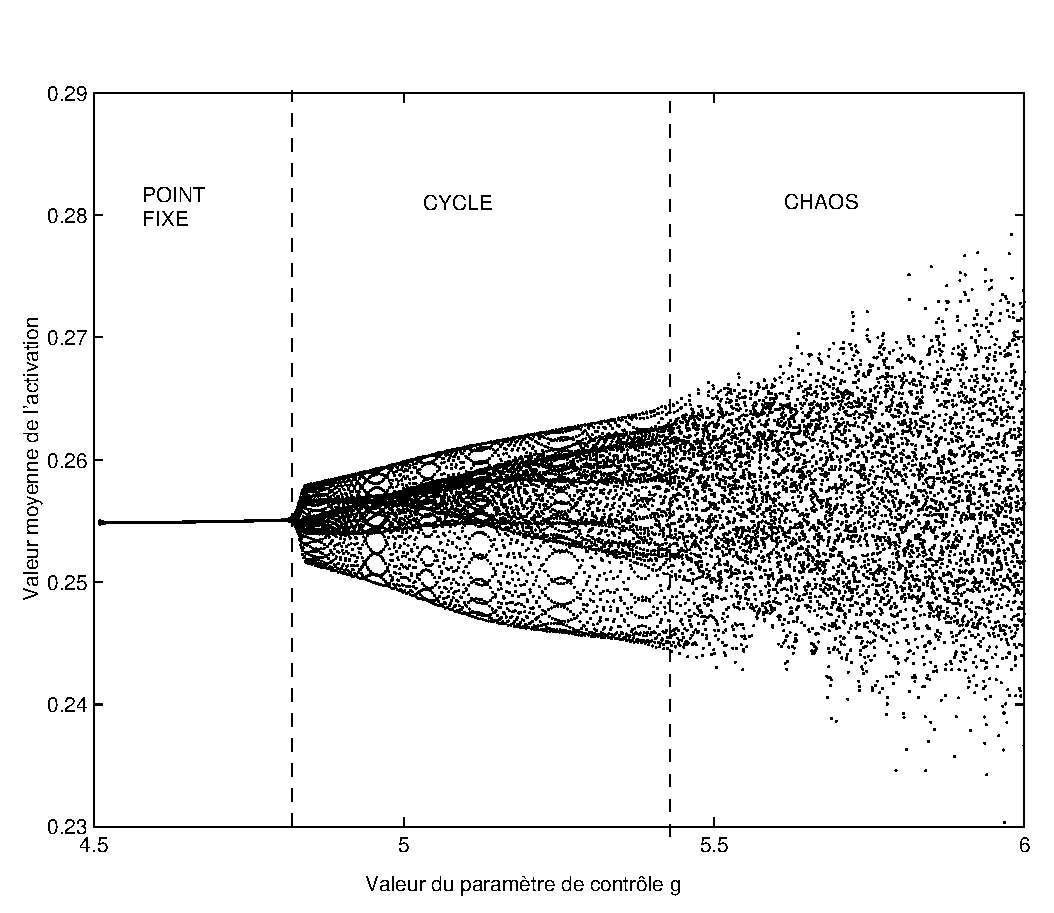
\includegraphics[width = 0.7\linewidth]{figs/hermes_diagr_bif.eps}
	}
	\caption{Transitions de phase.
		La figure représente l’activité moyenne d'un réseau récurrent aléatoire de 200 neurones sur 14 000 pas de temps,
		tandis que l’on augmente lentement le gain
		entre $g=4$ et $g=6$ (Beslon \& Daucé, 2002)}
	\label{fig:hermes-bif}
\end{figure} 


Il est intéressant de constater que le processus stochastique limite, tel que décrit par les équations de champ moyen, 
a une traduction à taille finie
sous la forme d'une activité de type \textit{chaos déterministe}. L'existence d'un 
paramètre de contrôle (le gain de la fonction de transfert des neurones) permet de reproduire, dans ces réseaux aléatoires, 
un  comportement générique de déstabilisation, appelé route vers le chaos par ``quasi-périodicité'' \shortcite{Berger1988,Doyon1993} (voir figure \ref{fig:hermes-bif}).
L'existence d'une telle frontière entre l'ordre et le chaos est également prouvée à la limite thermodynamique, mais dans ce
cas la transition se fait brutalement, avec un passage discret d'un processus de type point fixe à un processus stochastique \shortcite{Ces95}.
Cette frontière entre ordre et chaos est par principe intéressante puisqu'elle indique le lieu
où la variabilité de la dynamique, et donc potentiellement {\color{Orange} l'expressivité du réseau est la plus importante. }

\subsection{Réseaux équilibrés} \label{sec:balanced}

L'activité nerveuse est caractérisée par la présence fréquente d'oscillations collectives, souvent transitoires, 
observables à différentes échelles \shortcite{WangXJ2010}. 
%{\color{Orange} Le mécanisme par lequel une population de neurones peut se mettre à osciller 
%ont déjà été présentés dans la section \ref{sec:balanced}}. 

Les comportements oscillants ont été analysés de manière approfondie en modélisation à travers l'étude des réseaux de neurones dits ``équilibrés'' (\textit{balanced neural networks}).
Il s'agit d'une 
classe de réseaux de neurones constitués d'une population de neurones inhibiteurs et d'une population de neurones excitateurs.
Le terme ``équilibre'' se réfère ici à l'idée d'équilibre
dynamique entre deux forces opposantes~: la dynamique du réseau est amenée à converger vers un point d'équilibre
traduisant localement (et globalement) le ``poids'' des deux influences. 
\begin{itemize}
	\item Une configuration des poids se traduisant
	par une activité endogène soutenue 
	traduit une domination de l'influence excitatrice.
	\item A l'inverse, une configuration où l'activité intrinsèque disparaît après un certain temps 
	traduit une domination de l'influence inhibitrice.
\end{itemize} 

Comme dans le cas des réseaux aléatoires simples, il existe un paramètre de contrôle correspondant au rapport entre l'influence 
excitatrice et l'influence inhibitrice. 


De manière intéressante, une grande variété de comportements dynamiques peuvent être observés
à la frontière, et entre l'extinction et l'activité soutenue, comme les oscillations synchronisées \shortcite{brunel00} et/ou le chaos \shortcite{Van98}. 

\subsubsection{Rôle computationnel des oscillations synchronisées}
Plusieurs hypothèses ont été proposées sur le rôle
des oscillations synchronisées, 
\begin{itemize}
	\item comme mécanisme permettant de {\color{Orange} ``lier'' (assembler) les différentes modalités (constituants) d'un 
		même phénomène \shortcite{Gra89}}. La cohérence de phase
	observée à large échelle est vue comme la signature d'une activité coordonnée entre des aires séparées par plusieurs 
	centimètres \shortcite{Rod99}. 
	\item comme porteuse permettant une forme de cadençage et de séquençage des stimuli 
	dans les couches sensorielles primaires \shortcite{MLe96}. 
	\begin{itemize}
		\item Différents régimes oscillatoires sont classiquement identifiés, classifiés selon la
		bande de fréquence qu'ils occupent :  oscillations theta (3-8 Hz), oscillations alpha (10-15 Hz), oscillations beta (15-25 Hz) et
		oscillations gamma (> 30 Hz) \shortcite{Bremer1949}.
		\item L'anticipation de phase (phase précession) ou le retard de phase observés au niveau cellulaire dans 
		un contexte d'oscillations theta \shortcite{Skaggs1996}
		sont interprétés comme caractéristiques d'une activité au sein de laquelle l'ordre de tir 
		des potentiels d'action individuels joue un rôle important.
	\end{itemize}
\end{itemize} 

\subsection{Codage topographique et champ neuronal}\label{sec:NField}

Le modèle du ``champ neuronal'' est un modèle de type champ moyen, c'est à dire qu'il décrit les réseaux de neurones d'un point de vue macroscopique. L'activité de larges populations de neurones s'apparente en effet, à la limite des grandes tailles, à un milieu continu dans lequel chaque portion de l'espace peut être décrit par la ``densité'' d'activité qui s'y développe.

Le modèle le plus connu est décrit par des équation intégro-différentielles. Soit $x$ un point d'un espace (ou d'une portion d'espace) cartésien $\mathcal{X}$.
Dans le modèle d'Amari \shortcite{Ama77B}, les neurones sont décrits par leur potentiel d'activation $V$ et par la sortie binaire de la fonction d'activation $f$ (fonction de Heaviside).  Le potentiel d'activation d'un neurone est donné par l'équation~:
\begin{align}
\tau \frac{dV(x,t)}{dt} = -V(x,t) + I(x,t) - \theta + \int_{y \in \mathcal{X}} W(||x-y||) f(V(y,t)) dy
\end{align} 
où $I$ est un signal extérieur et $W$ un noyau décrivant les interactions réciproques entre neurones en fonction de la distance $||x - y||$.


{\color{Cyan}
{\bf!! Attention répétitions!!}

Le codage topographique est une des manière d'exprimer des grandeurs
continues dans un substrat neuronal. 
Il s'apparente au calcul par champ (``Field computation'' \cite{Maclennan1999})
consistant à étudier des mécanismes de calcul à partir de 
modèles d'interaction basés sur la physique des milieux continus. 
Le débat n'est pas tranché à l'heure actuelle pour savoir si l'activité neuronale, 
par nature discrète, traduit les grandeur continues de manière \emph{qualitative} 
(différents neurones étant assignés à différentes valeurs - ou intervalles) 
ou \emph{quantitative} (chaque neurone
pouvant exprimer plusieurs valeurs par sa fréquence de décharge).
Le système visuel primaire, organisé autour de la topographie de la rétine, semble par exemple 
obéir à une organisation de type qualitatif où les différentes coordonnées
du champ visuel sont assignées à des populations de neurones distinctes \cite{HUBELWIESEL62}. 
L'étude des zones motrices primaires plaident plutôt pour un caractère quantitatif de l'activité motrice,
la contraction des muscles étant proportionnelle au taux de décharge.

Le modèle fondateur du codage topographique est le champ neuronal (``Neural Field'') d'Amari \shortcite{Ama77B},
déjà mentionné dans la section \ref{sec:NField}. Selon le noyau choisi, le réseau développe un ou plusieurs 
foyers d'activité métastables  interprétables au choix comme un patron d'activité ou comme un
ensemble de grandeurs scalaires (en fonction des barycentres des foyers d'activité).
Le codage topographique est la manière la plus naturelle de représenter les signaux sensoriels 
dans les architectures neuronales.
Il correspond également aux observations sur l'organisation des couches sensorielles primaires (à l'exception de l'olfaction).



La vocation des modèles de champ neuronal \shortcite{Ama77B} est principalement la modélisation d'un substrat neuronal spatialisé vu à ``large échelle'' 
(continuum d'activité sur la surface corticale).
Ce modèle partage avec le réseau de Hopfield \cite{Hop82} la capacité à conserver et entretenir 
une activité autonome indépendamment de son signal d'entrée. 
Il implémente néanmoins des opérations tout à fait spécifiques et intéressantes du point de vue computationnel. 
Un champ neuronal implémente simultanément une ``mémoire de travail'' (capacité à conserver la trace d'une stimulation passée), et 
un mécanisme de traitement (ici résumé à quelques opérations simples : émergence, extinction, fusion, poursuite) \shortcite{Schoner95}. 
La combinaison de ces deux compétences (mémoire et calcul)
au sein d'une architecture unique fait en principe du neural field un environnement computationnel complet \shortcite{Siegelmann1999,Maclennan1999,Potthast2013}. 

L'avantage du codage topographique est sa plus grande expressivité. 
Un foyer d'activité unique sur un substrat 
bidimensionnel exprime ainsi une grandeur vectorielle (typiquement la position d'une cible sur une rétine).
Les patrons d'activité plus complexes observés dans les couches primaires \shortcite{Bonhoeffer1991} caractérisent des relations spatiales entre des contours
difficiles à exprimer à l'aide de simples neurones fréquentiels.
Les caractéristiques du codage topographique suggèrent par ailleurs des mécanismes
de contrôle de type ``point fixe'' où la commande motrice est définie comme le point d'équilibre 
entre différentes postures dans l'espace des tâches \shortcite{Schoner95,Mussa2004,Flash2005}. 
Cette théorie permet d'expliquer comment les
variations d'activité, en agissant linéairement sur les différentes forces, ne déplacent pas le point d'équilibre.

Le codage topographique suggère également un apprentissage ``par coeur'' des relations 
métriques entre les différents 
référentiels sensoriels (extéroceptifs ou proprioceptifs) \cite{Pouget1997}. 
Dans ce schéma, la conséquence proprioceptive d'une commande motrice 
visuelle (excentricité finale de l'oeil dans le globe oculaire suite 
à une saccade oculaire par exemple) doit être appris par
essai/erreur. 

Le codage topographique joue par ailleurs un rôle qui s'apparente à celui des fonctions noyau utilisées en 
apprentissage automatique \shortcite{Scholkopf2002}.
Le plongement des données d'entrée dans un espace de fonctions à noyau reproductible garantit en effet 
l'existence d'un hyperplan séparateur permettant la discrimination des données.
Cette meilleure séparabilité des données est obtenue au prix d'une augmentation de
la complexité du classifieur (dimension de Vapnik).
Dans le cas des architectures neuronales, le codage topographique repose sur l'activité 
de larges populations de neurones, et
représente donc un coût plus élevé que le codage fréquentiel, 
en principe implémentable sur un neurone isolé. 


}

\subsubsection{Rôle computationnel du codage topographique}


\subsection{Neurones impulsionnels}
%%%%%%%%%%%%%%%%%%%%%%%%%%%%%%%%%%%%%%%%%%%%%%%%%%%%%%%%%%%%%%%%%%%%%%%%%%%%%%%%%%%%%%%%%%%%%%%%%%%%%%%%%%%%%%%%%%%

\paragraph{Intégration sous-liminaire}
 Les neurones biologiques
 ont un comportement fortement non-linéaire, caractérisé par le franchissement d'un seuil d'activation.
 La cellule neuronale intègre les multiples potentiels post-synaptiques issus de ses synapses afférentes
 et émet un bref potentiel d'action lorsque le potentiel total atteint le seuil d'activation (on
 dit que la membrane se dépolarise).
 Après une brève période de repos (``remise à zéro''), le neurone recommence à intégrer les signaux entrants etc.

\paragraph{Action et contre-action}
Les neurones biologiques sont également caractérisés par le type de neurotransmetteurs qu'ils émettent
au niveau des synapses de leur arborisation terminale. On distingue les neurones inhibiteurs produisant des
synapses GABAergiques et les neurones excitateurs produisant des synapses excitatrices variées 
(glutamate, acétylcholine, dopamine, ...). 
L'action synaptique inhibitrice est une ``contre-action'' qui vient s'opposer
à l'effet des synapses excitatrices.

L'action et la contre-action, c'est à dire l'équilibre dynamique entre
deux forces opposées, est au coeur des opérations réalisées par le système nerveux. 

\paragraph{Rôle computationnel}
Les neurones à potentiel d'action disposent en principe d'une expressivité 
supérieure à celle des neurones à fréquence de décharge \shortcite{Izh06}.
Ils offrent des possibilités d'opérations (tels le codage par rang, la polychronisation,...)
ainsi qu'un support pour un traitement parallèle distribué (``multiplexage'') par décalage de phase
ou par bande de fréquences \shortcite{Skaggs1996,wang96gamma,Wang2010}. % [CITATIONS].
Un des enjeux connus est la possibilité d'émuler un mécanisme de synchronisation/coordination 
longue distance supposé à l'oeuvre dans le cerveau pour l'integration multimodale \shortcite{Rod99}.





%\subsection{Applications}

%\cleardoublepage

\section{Contributions personnelles}

{\color{Cyan}
	Par rapport aux propositions, j'ai fait:
	\begin{itemize}
		\item ceci
		\item {\color{Orange} Proposition~: la présence d'une pulsation périodique permet d'implémenter les propriétés du neural field sans utiliser de mémoire cellulaire.}
		\item etc.
	\end{itemize}
}	

\subsection{Réseaux aléatoires multi-populations}\label{sec:multi_pop}
Une des premières études auxquelles j'ai participé portait sur les transitions de phase dans les réseaux de neurones
aléatoires. 
Les différentes architectures neuronales étudiées ont 
permis d'identifier des comportements caractéristiques, décrits sous la forme de différents régimes dynamiques. 
{\color{Orange} Nous avons cherché à caractériser l'expressivité de ces substrats, c'est à dire leur capacité à produire
des patrons d'activité pouvant servir de support à des opérations cognitives. }

\begin{figure}[b!]
	\centerline{
		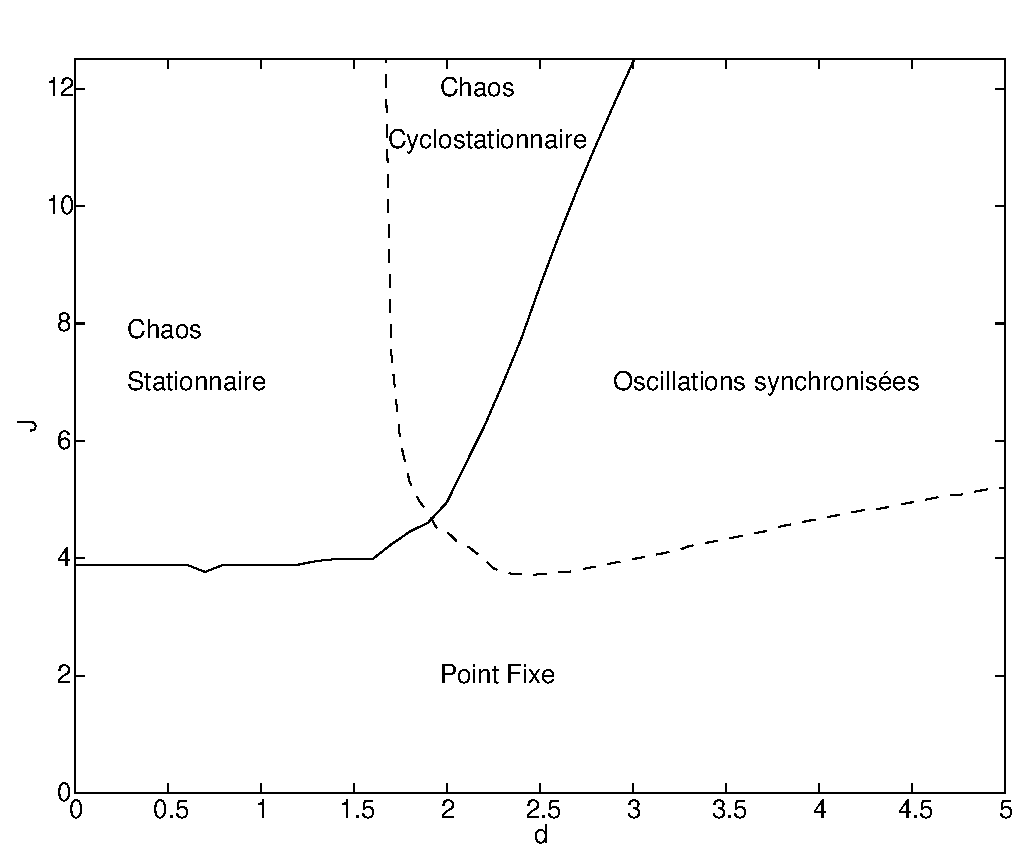
\includegraphics[width = 0.7\linewidth]{figs/map_2pop.eps}
	}
	\caption{Diagramme de bifurcation à la lite thermodynamique sur un réseau aléatoire équilibré à 2 populations, en fonction de $d$ (homogénéité) et $J$ (amplification).}
	\label{fig:diagr-2pop}
\end{figure} 

L'étude présentée dans \shortcite{Dau99A,dauce01a} étudie le comportement d'un réseau dit ``équilibré'' (voir section \ref{sec:balanced}). 
{\color{Gray} Le point de départ consistait à modéliser et reproduire certains comportements observés dans les 
réseaux de neurones naturels composés d'une population de neurones excitateurs et d'une population de neurones inhibiteurs (réseaux équilibrés,.}
Ce papier 
étend pour la première fois le modèle de champ moyen pour le cas des réseaux à connectivité aléatoire à populations multiples
(auquel cas les tirages aléatoires sont effectués sur des ``faisceaux d'axones'' reliant une population de neurones $p \in 1..K$ à une
population de neurones $q \in 1..K$, où $K$ est le nombre de populations).
Ce modèle renouvelle l'approche large-échelle classique \shortcite{WILSON89} en prenant en compte l'hétérogénéité des faisceaux
d'axones reliant différentes régions du réseau.  
Il sert de base à la définition d'architectures neuronales fondées sur des 
substrats à connectivité aléatoire. 

%{\color{Violet}
%[Multi-pop = base pour l'approche multi-échelle. Construction / architecture neuronale. Prise en compte de l'hétérogénéité.]
%Multi-pop = travail de master d'O Pinaud.
%Demonstration champ moyen = O Moynot (avec généralisation à la connectivité diluée)}

L'étude numérique proposée dans le papier fixe le rapport excitation/inhibition à $\frac{1}{2}$,
ce qui correspond à un régime de faible activité \shortcite{Amit1989}. 
Nous étudions le rôle contrasté de deux paramètres de contrôle (voir Figure \ref{fig:diagr-2pop}). 
\begin{itemize}
	\item Le premier paramètre, $J$, représente l'amplification du signal. L'augmentation
	continue de ce paramètre tend à produire une bifurcation entre un régime simple (point fixe) et une activité 
	complexe (de type chaotique) {\color{Orange} comme précédemment.}
	\item Un second paramètre, nommé $d$, représente l'inverse du \textit{coefficient de variation} des liens, autrement dit le 
	degré d'homogénéite. Augmenter ce paramètre tend à rendre les poids plus homogènes. 
\end{itemize}
De manière intéressante, 
l'augmentation continue de ce second paramètre (augmentation de l'``ordre'') produit une transition 
entre un régime stationnaire et un régime non-stationnaire périodique. Nous mettons en évidence une carte
de bifurcation à 4 régions, comprenant un régime stationnaire de point fixe, un régime stationnaire complexe,
un régime d'oscillations simple, et un régime d'oscillations complexes analogue à processus stochastique cyclostationnaire,
ce dernier régime étant à notre connaissance mis en évidence pour la première fois dans ce type de réseaux.





Notre étude a donc ouvert la voie à l'étude multi-population systématique des réseaux de neurones à connectivité aléatoire,
voir par exemple \shortcite{Faugeras2009,Cabana2013}. %L'accent sur l'équilibre dynamique entre populations escitatrice et inhibitrice

{\color{Orange}[CITER SOULA-BESLON] et ECM avec IF neurons}


%{\color{Violet}
%[O. Faugeras, J. Touboul, B. Cessac, “A constructive mean field analysis of multi population neural networks with random synaptic weights and stochastic inputs”, Front. Comput. Neurosci. (2009) 3:1.

%et aussi 

%Large Deviations, Dynamics and Phase Transitions in Large Stochastic and Disordered Neural Networks
%Tanguy Cabana1 and Jonathan Touboul (2013)

%La question de l'homogénéité/hétérogénéité est revenue à l'ordre du jour. Plusieurs papiers récents bla bla...}



%\cleardoublepage
\subsection{Criticalité dans les réseaux aléatoires}\label{sec:criticalite}

Un des intérêts principaux des réseaux à connectivité aléatoire est leur capacité à générer des dynamiques complexes
endogènes (donc sans stimulation extérieure). Ces dynamiques, bien que reposant sur des équations déterministes,
se comportent comme des processus stochastiques indépendants sur chaque neurone. Ce comportement n'est pourtant pas analogue
à un simple bruit passif. 

\begin{figure}[b!]
	\centerline{
		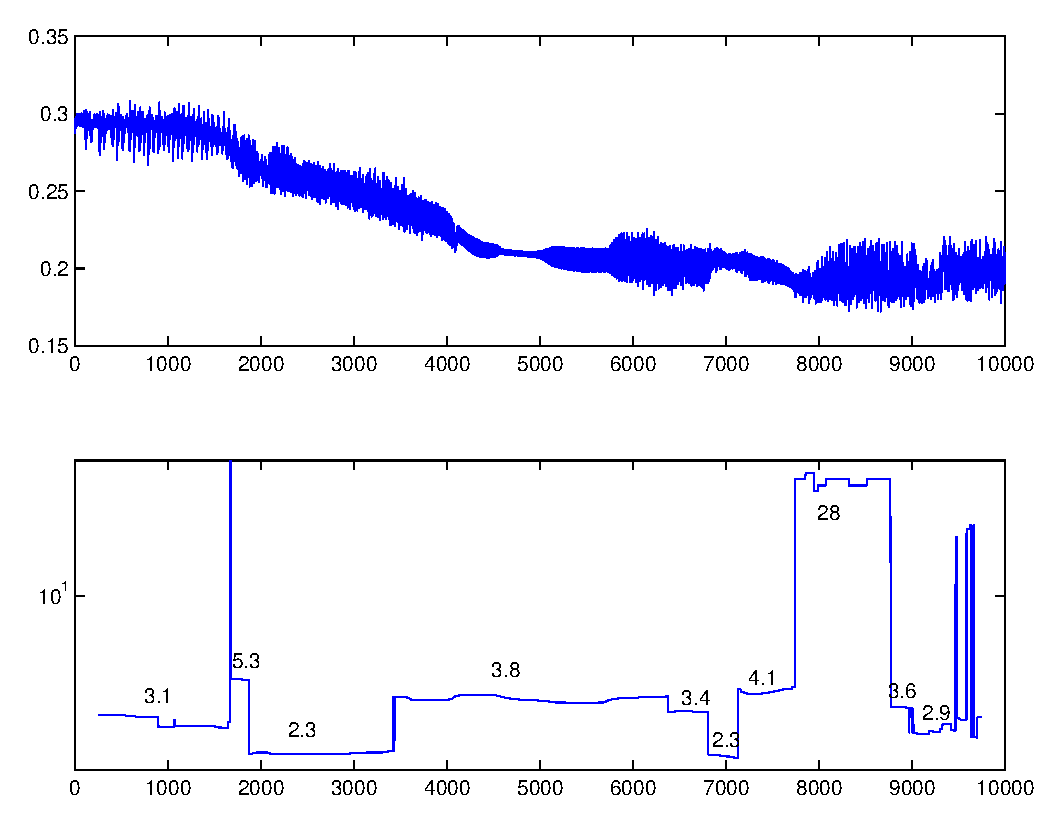
\includegraphics[width = 0.7\linewidth]{figs/simu_derive_periodes_x2.eps}
	}
	\caption{Activité d'un réseau récurrent aléatoire de 200 neurones, sur 10000 pas de temps, sous l’influence d'une entrée sensorielle à évolution lente. La période principale est estimée par spectre de Fourier sur
		une fenêtre de 500 pas de temps (cette période étant représentative de la période propre de
		chaque neurone actif). a) Activité moyenne. b) 
		Période du mode principal (en échelle logarithmique) (Beslon \& Daucé, 2002)}
	\label{fig:hermes-critic}
\end{figure} 


Une manière simple de caractériser le comportement non-linéaire (ou critique) d'une population de neurones consiste à introduire de petites perturbations
dans la dynamique du réseau. 
Une étude proposée dans le 3ème chapitre de l'ouvrage que nous avons co-dirigé avec Agnès Guillot \shortcite{Beslon2002} illustre le propos.
Cette étude porte sur le modèle le plus simple, un réseau récurrent aléatoire comportant une seule population. Le paramètre de contrôle
choisi place le réseau dans une région chaotique, proche de la transition vers le cycle limite.  
Le réseau est soumis à une stimulation extérieure quasi stationnaire, évoluant à une vitesse très lente par rapport à la vitesse de 
mise à jour du réseau. Une succession de régimes dynamiques distincts, séparés par des transitions brusques, est mise en évidence (voir figure \ref{fig:hermes-critic}).
Chaque régime est caractérisé par un patron d'activité différent, qui se manifeste par la présence de fréquences caractéristiques
distinctes dans le spectre de Fourier du signal moyen. 

% DONNEES A REPRENDRE SUR SIMU99_0726.mat
\begin{figure}[b!]
	\centerline{
		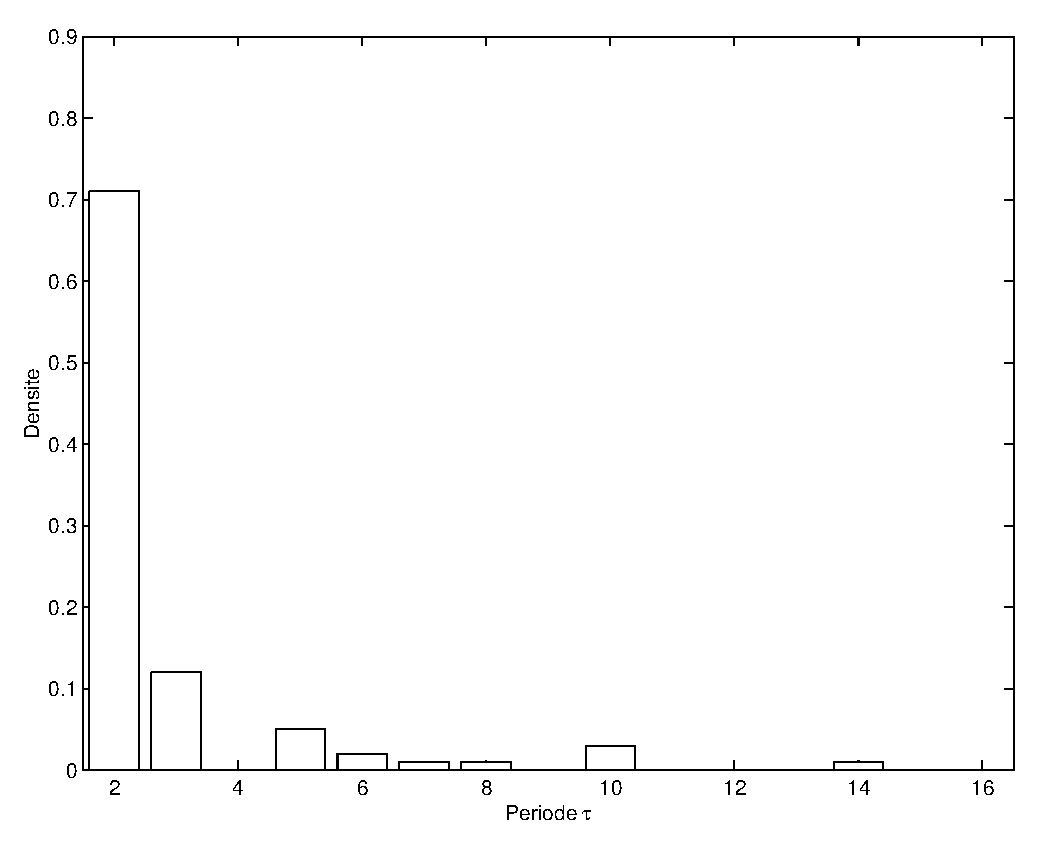
\includegraphics[width=0.3\linewidth]{figs/hist_periode_2.eps}
		\hspace{0.5cm}
		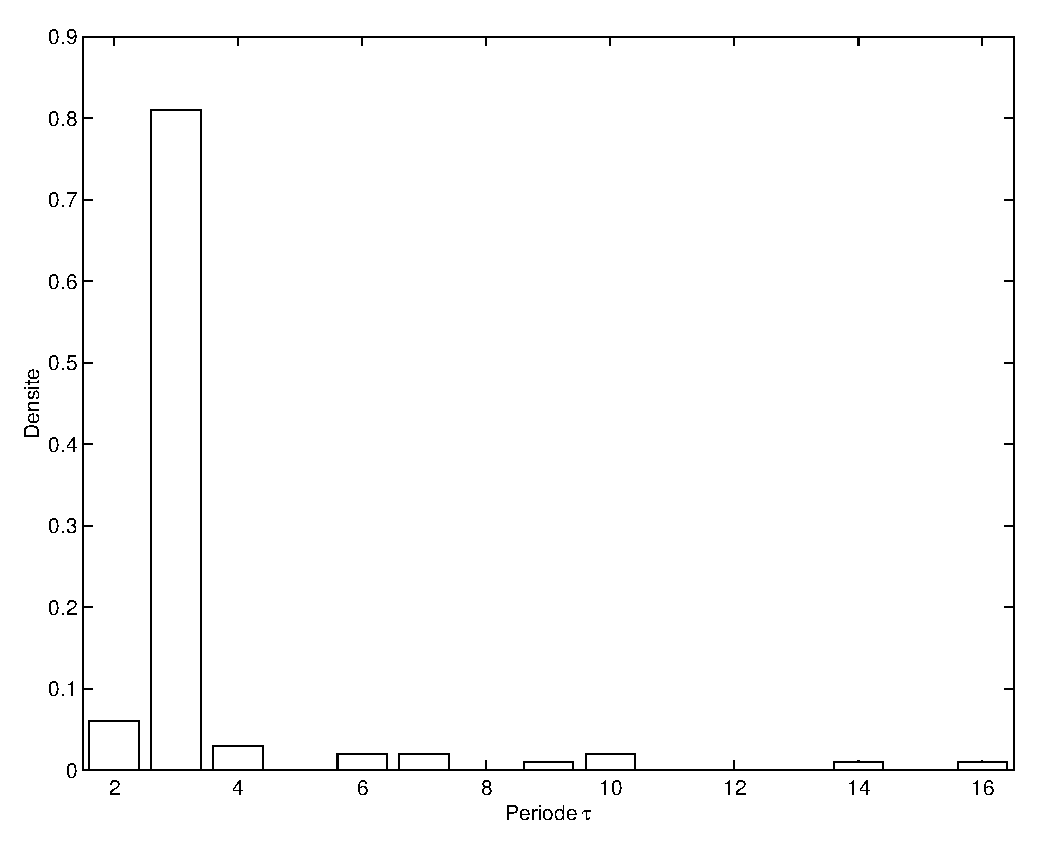
\includegraphics[width=0.3\linewidth]{figs/hist_periode_3.eps}
		\hspace{0.5cm}
		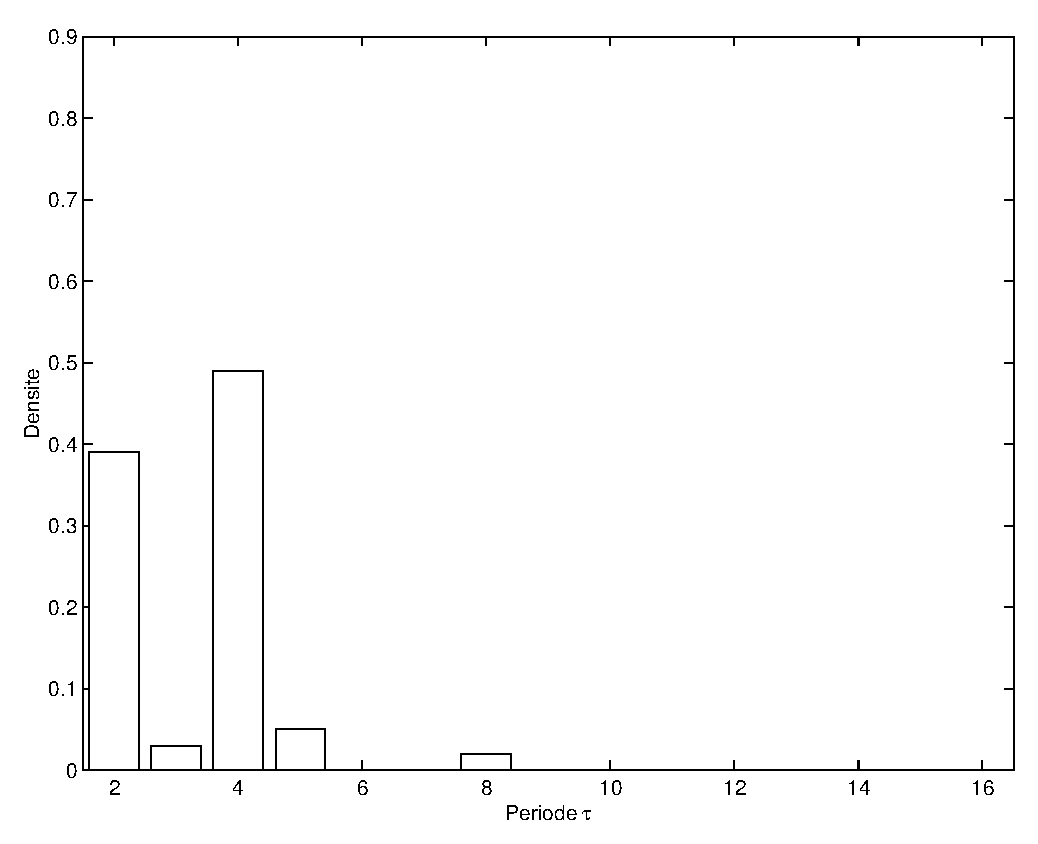
\includegraphics[width=0.3\linewidth]{figs/hist_periode_4.eps}
	}
	\centerline{
		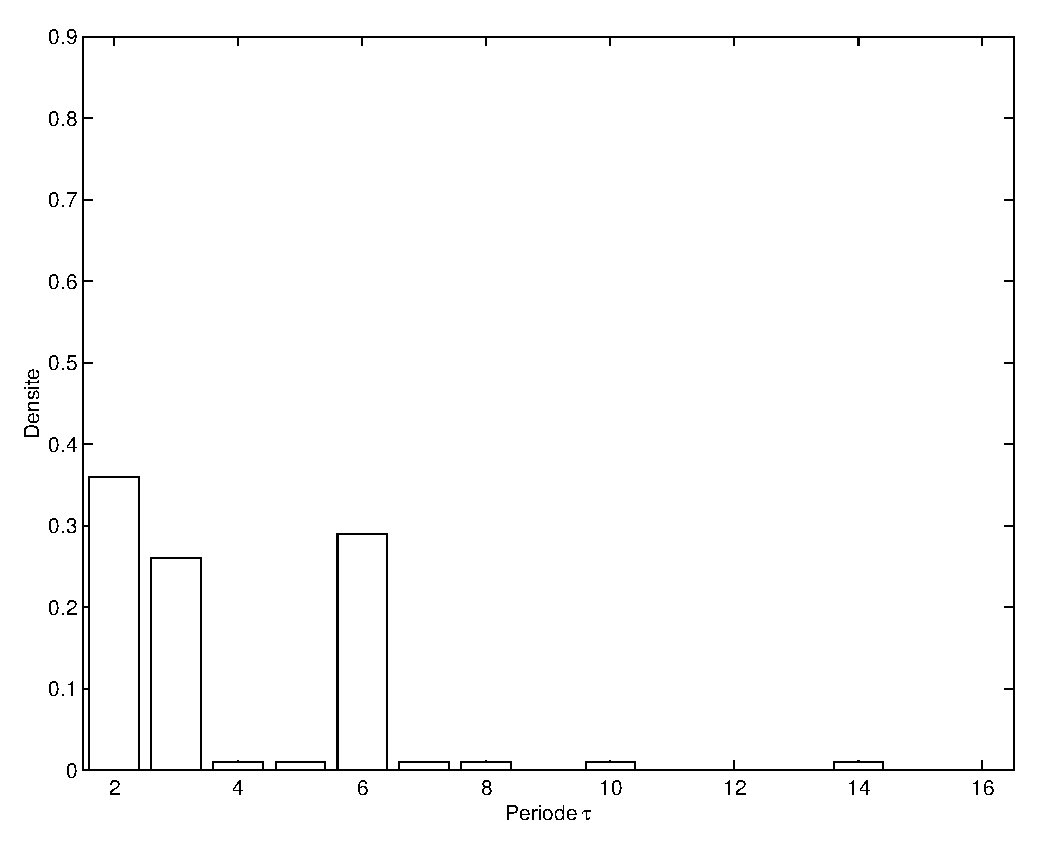
\includegraphics[width=0.3\linewidth]{figs/hist_periode_6.eps}
		\hspace{0.5cm}
		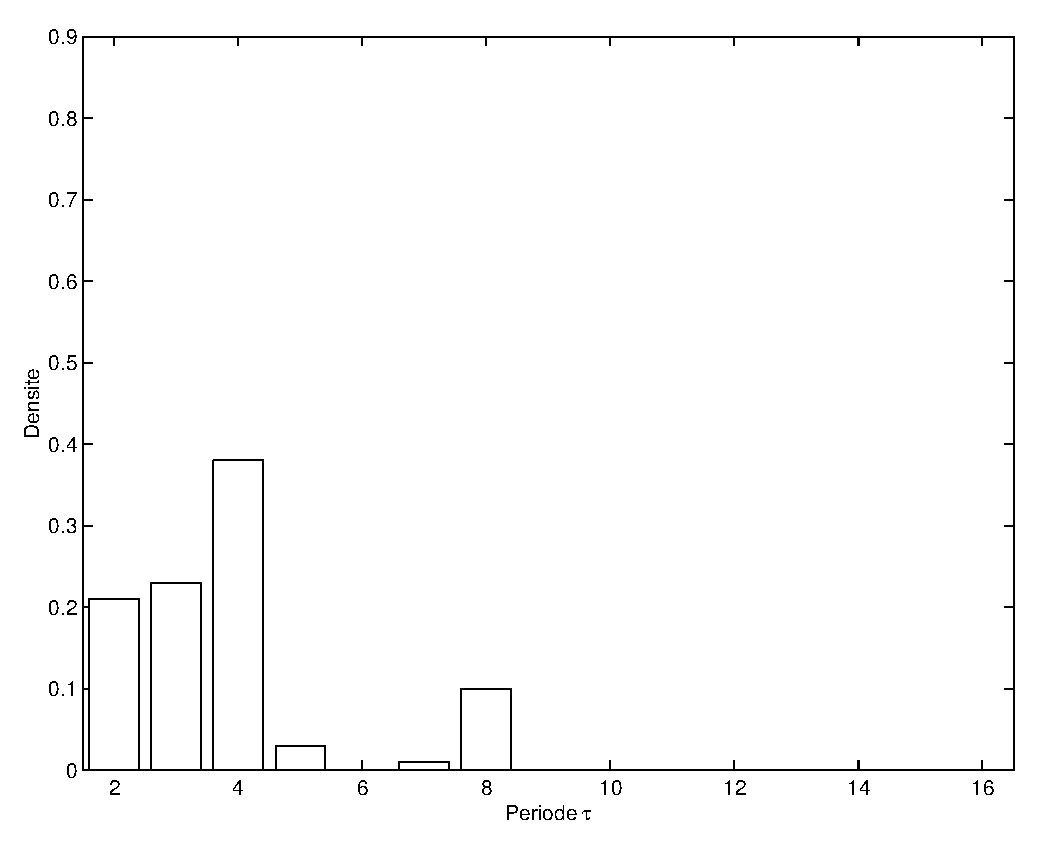
\includegraphics[width=0.3\linewidth]{figs/hist_periode_8.eps}
		\hspace{0.5cm}
		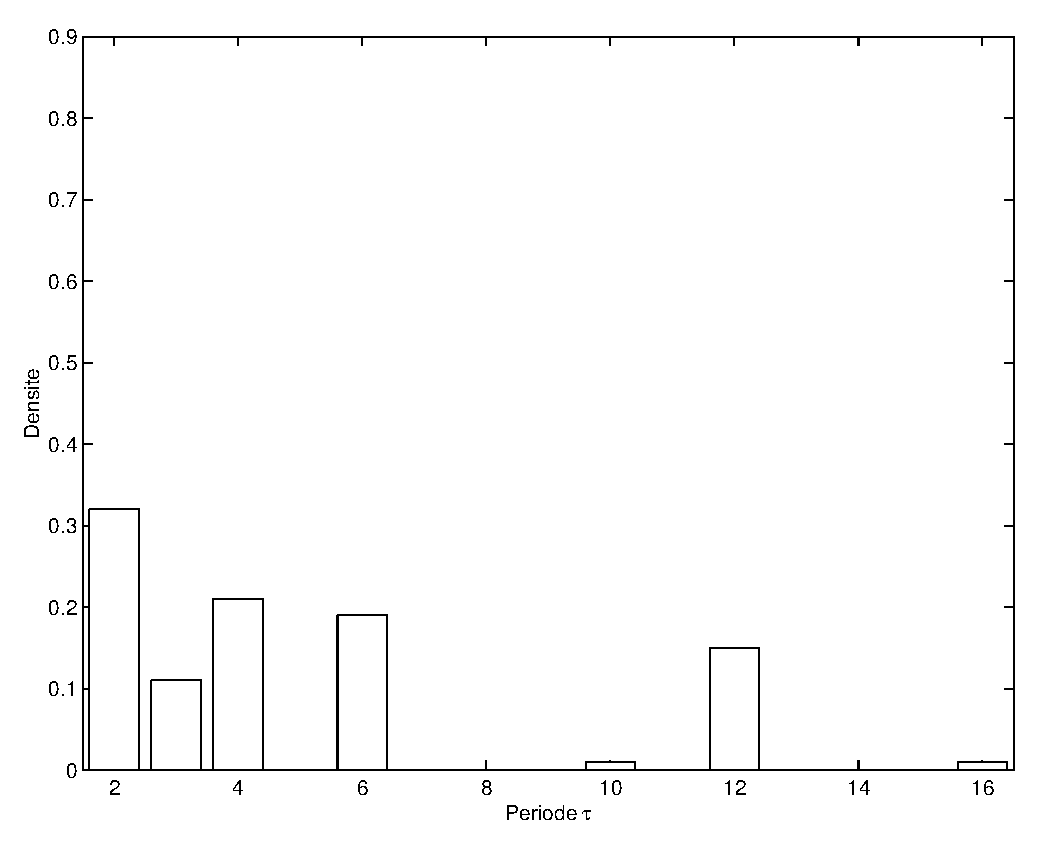
\includegraphics[width=0.3\linewidth]{figs/hist_periode_12.eps}
	}
	\caption{{\bf Capture de p\'eriode pour diff\'erentes valeurs de $\tau$ (période du signal).}
		On a repr\'esent\'e sur ces histogrammes la r\'epartition des p\'eriodes, mesur\'ee sur 100 couples (r\'eseau, s\'equence d'entrée) pour $\tau=2$ (haut, gauche), $\tau=3$ (haut, milieu), $\tau=4$ (haut, droite), $\tau=6$ (bas, gauche), $\tau=8$ (bas, milieu) et $\tau=12$ (bas, droite).
		Param\`etres~: $N=200$, $g=8$, $\bar{I}=0$, $\mu_{\theta}=0$, $\sigma_\theta=0$, $\mu_{J}=0$, $\sigma_J=1$, $\sigma_I=0.1$ (Daucé, 2001).
	}
	\label{fig:periode_expl}
\end{figure}


Une autre étude, présente dans mon manuscrit de thèse \shortcite{Dau00}, développe l'analyse spatio-temporelle des patrons d'activité de type cycle limite
ou chaos léger.
L'existence d'une chaîne d'activation spontanée (synfire chain \shortcite{ABELES91}) est mise en évidence par analyse de la matrice de covariance des signaux individuels. 
Différents modes (patrons d'activation spatio-temporels) se développent spontanément lorsque le réseau est soumis à des entrées statiques différentes \shortcite{Dau00b}.
Enfin, l'analyse de la réponse du réseau à une stimulation périodique indique une ``bande passante'' de quelques unités temporelles, le réseau étant capable 
de ``capturer'' (et donc d'amplifier) des signaux dont la période varie entre 2 et 10\--12 unités de temps
(autrement dit à sélectionner un mode dynamique périodique interne compatible avec la période imposée) \shortcite{Dau00b} \--- voir figure \ref{fig:periode_expl}.
Le comportements spontané des réseaux récurrents aléatoires est par ailleurs à la base du mécanisme de perception par feedback positif
présentés dans la section \ref{sec:BioCyb02}. 

L'intérêt du comportement spontané des réseaux récurrents à connectivité aléatoires a été largement confirmé depuis. 
Une étude plus systématique de la réponse linéaire dans les réseaux récurrents \shortcite{Cessac2007} met en évidence 
l'existence de modes et de résonances extrêmement variés lorsque le signal est applique sur un seul noeud du réseau (micro-stimulation). 
Les modèles de ``réservoir
computing'' proposés par l'équipe de Wolfgang Maas \shortcite{Maass2002} reposent sur le même principe : un réseau de neurones aléatoire récurrent soumis à un signal
spatio-temporel est capable de conserver une mémoire de quelques unités de temps utilisables pour produire des classifieurs sensibles
au contexte temporel.

{\color{Cyan} Image du papillon-chenille.}

Ce modèle de réseau à connexions aléatoire offre un exemple de substrat dont la caractéristique principale est la \textit{capture dynamique}, reposant
sur des transformations morphologiques des patrons d'activités (changements des distributions spatiales et temporelles des activités). Bien que construits sur
un tirage aléatoire arbitraire, ils offrent donc un bon support pour le traitement (et la transformation) des signaux temporels. 
Faire reposer le traitement sur un tirage arbitraire rejoint d'ailleurs un certain nombre de techniques de plongement (ou projection) aléatoires
utilisées en apprentissage automatique, tels le ``compressive sensing'' \shortcite{Baraniuk2007} ou l'architecture ``extreme learning'' \shortcite{Huang2006}.

%%\cleardoublepage
%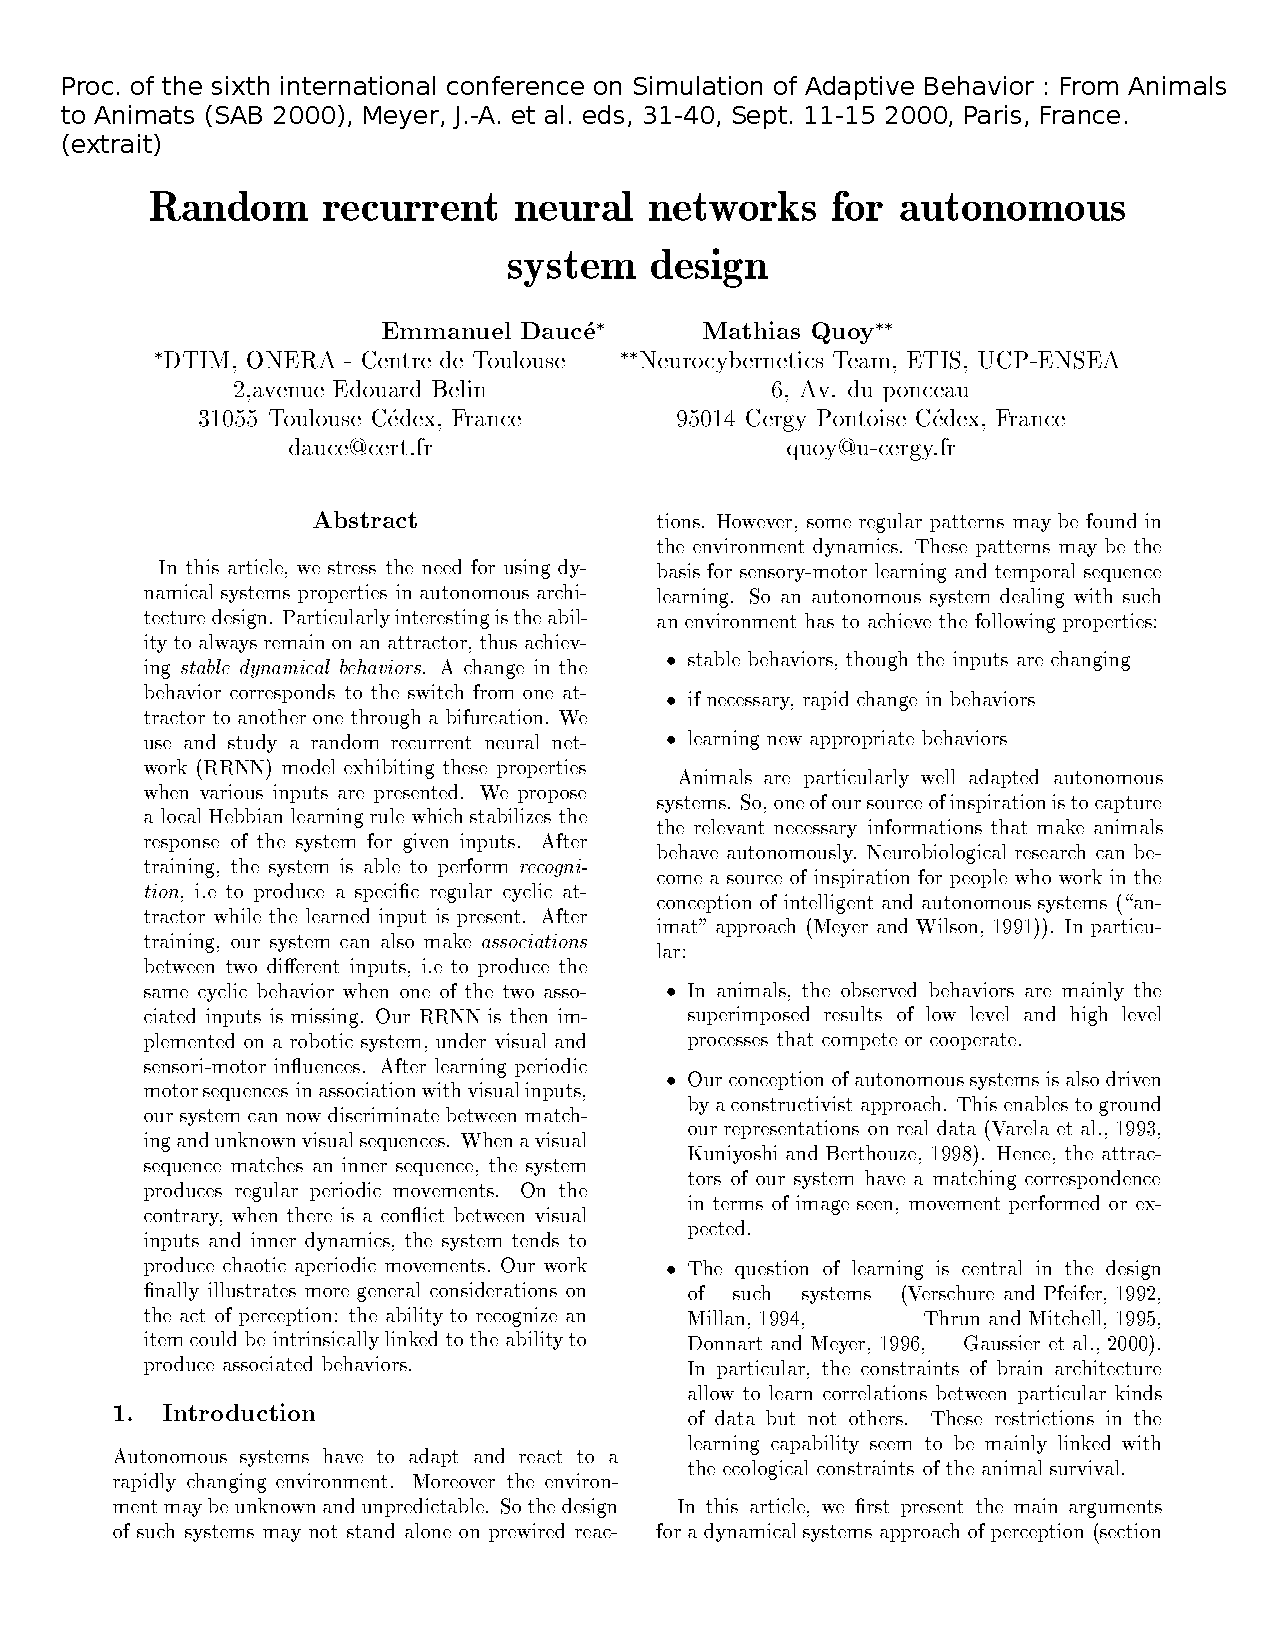
\includepdf[pages=1, offset=70 -20]{pdf/2000-sab-ann.pdf}
%\includepdf[pages=2, offset=-70 -20]{pdf/2000-sab-ann.pdf}
%\includepdf[pages=3, offset=70 -20]{pdf/2000-sab-ann.pdf}
%\includepdf[pages=4, offset=-70 -20]{pdf/2000-sab-ann.pdf}
%\includepdf[pages=18, offset=70 -50]{pdf/2007-epj-st-ann2.pdf}
%\includepdf[pages=19, offset=-70 -50]{pdf/2007-epj-st-ann2.pdf}
%\includepdf[pages=20, offset=70 -50]{pdf/2007-epj-st-ann2.pdf}
%\includepdf[pages=21, offset=-70 -50]{pdf/2007-epj-st-ann2.pdf}
%\includepdf[pages=22, offset=70 -50]{pdf/2007-epj-st-ann2.pdf}
%\includepdf[pages=23, offset=-70 -50]{pdf/2007-epj-st-ann2.pdf}
%%%%%%%%%%%%%%%%%%%%%%%%%%%%%%%%%%%%%%%%%%%%%%%%%%%%%%%%%%%%%%%%%%%%%%%%%%%%%%%%%%%%%%%%%%%%%%%%%%%%%%%%%%%%%%%%%%%
%%%%%%%%%%%%%%%%%%%%%%%%%%%%%%%%%%%%%%%%%     1.3      %%%%%%%%%%%%%%%%%%%%%%%%%%%%%%%%%%%%%%%%%%%%%%%%%%%%%%%%%%%%
%%%%%%%%%%%%%%%%%%%%%%%%%%%%%%%%%%%%%%%%%%%%%%%%%%%%%%%%%%%%%%%%%%%%%%%%%%%%%%%%%%%%%%%%%%%%%%%%%%%%%%%%%%%%%%%%%%%

%%%%%%%%%%%%%%%%%%%%%%%%%%%%%%%%%%%%%%%%%%%%%%%%%%%%%%%%%%%%%%%%%%%%%%%%%%%%%%%%%%%%%%%%%%%%%%%%%%%%%%%%%%%%%%%%%%%
%%%%%%%%%%%%%%%%%%%%%%%%%%%%%%%%%%%%%%%%%     1.2      %%%%%%%%%%%%%%%%%%%%%%%%%%%%%%%%%%%%%%%%%%%%%%%%%%%%%%%%%%%%
%%%%%%%%%%%%%%%%%%%%%%%%%%%%%%%%%%%%%%%%%%%%%%%%%%%%%%%%%%%%%%%%%%%%%%%%%%%%%%%%%%%%%%%%%%%%%%%%%%%%%%%%%%%%%%%%%%%

%\cleardoublepage
\subsection{Modèles de champ neuronal}\label{sec:NatComp}

La question adressée par le modèle publié en 2004 \shortcite{Dau04} est celle de l'implémentation d'un modèle de champ neuronal (voir section \ref{sec:NField}) sur un support composé
d'unités discrètes.
%, comme l'activité dite ``persistante'' ainsi qu'une bonne sensibilité au signal d'entrée (switch). 
Sur les modèles jusqu'alors proposés, dans un cas l'activité focale était soit uniquement réactive \shortcite{Han96},  
dans l'autre cas,
l'activité persistante reposait sur un mécanisme de bistabilité cellulaire \shortcite{Cam98} ou encore sur une
plasticité synaptique à court terme \shortcite{Com00}. 
Notre modèle est une des premières implémentations d'un champ neuronal sur support discret reposant sur des mécanismes de réseau
uniquement.

Le papier étend le modèle récurrent aléatoire \shortcite{Dau01a} à des connectivités
plus complexes, incluant des délais variables et les connexions dépendantes de la distance. 
Un des apports du papier est de montrer 
la stabilité de certains indicateurs (comme le niveau de réponse moyen) à travers les modèles. 
Par exemple, l'introduction de délais différents entre les populations excitatrices et les populations inhibitrices conduit 
à des changements qualitatifs (régime d'oscillations lentes synchronisées) mais non quantitatif (même réponse
moyenne). 

L'introduction d'une connectivité dépendante de la distance opère un changement plus radical, 
puisque l'hypothèse fondatrice du modèle (indépendance des tirages) n'est plus vérifiée, 
et donc l'hypothèse de chaos local (indépendance des activités) n'est plus valide.
Les unités neuronales de chaque population reçoivent des coordonnées spatiales (ici prises uniformément sur un intervalle borné). %$[-\pi,\pi]$).
Le tirage des poids synaptiques devient dépendant de la distance qui sépare deux unités.
La valeur moyenne d'un poids est identique à celle du modèle précédent, 
mais les noeuds les plus proches ont en espérance une valeur
plus forte, et les noeuds les plus éloignés une valeur plus faible 
(la distribution des poids synaptiques repose sur le produit
entre la distribution uniforme initiale et un noyau gaussien conservatif).
Le mécanisme du champ neuronal, qui se caractérise par une connectivité majoritairement excitatrice à 
courte distance, et inhibitrice à longue distance, est implémenté à l'aide de ces noyaux gaussiens 
tels que le rayon du noyau des liens excitateurs est plus faible que celui des liens inhibiteurs.  

Le papier montre alors que les propriétés des réseaux aléatoires récurrents et celles des champs neuronaux s'additionnent dans ce modèle,
puisqu'on peut mettre en évidence sur ce substrat la présence simultanée d'une activité de fond chaotique,
de grandes oscillations lentes et de foyers d'activité de type champ neuronal. 
Comme dans le cas du champ neuronal, l'activité persistante repose sur l'activité excitatrice locale, avec 
un effet de lissage lié à l'hétérogénéité des connexions. Les oscillations lentes reposent comme précédemment
l'existence de délais différenciés. Ce sont ces oscillations qui donnent au substrat 
la capacité de répondre à des changements de faible amplitude (augmentent donc la sensibilité 
du substrat au signal d'entrée). Il en résulte une implémentation d'un champ neuronal 
sur un substrat composé d'unités neuronales discrètes.

De manière plus générale, ce modèle nous fournit un premier exemple, dans le cadre des réseaux récurrents aléatoires,
de l'effet de mémoire produit par une boucle de rétroaction positive. 

Notre modèle propose une passerelle simple entre les modèles de champ neuronal continus et de
réseaux de neurones à état et à temps discret. 
Il s'étend facilement à des réseaux de neurones intègre-et-tire (non publié), avec des
%L'activité produite repose néanmoins essentiellement sur la fréquence de tir des neurones (et non sur l'ordre de tir
%ou la co-activation). Les propriétés obtenues ne sont donc 
propriétés peu différentes qualitativement de celles qu'on 
obtient avec des modèles à fréquence de décharge.
Ce modèle a été utilisé en tant que couche perceptive dans des architectures de contrôle \shortcite{Dau04b,Dau07}. 
D'autres modèles visant une plus grande fidélité aux processus biologiques 
ont étudié l'effet de délais variables et de patrons de connexion hétérogènes (voir par exemple \shortcite{Roxin2005}),
et plus généralement l'étude de l'interaction entre délais variables, topographie et dynamique reste un sujet d'actualité 
en neurosciences computationnelles \shortcite{Voges2012,Lundqvist2012}.

\subsection{Extension aux populations de neurones impulsionnels}

{\color{Violet}
Le passage des neurones binaires aux neurones à potentiels d'action 
modifie la nature des régimes dynamiques produits par le réseau. Une différence importante avec les modèles à sortie 
continue est la définition précise de l'échelle temporelle sur les délais de transmission comme sur 
les constantes de temps et les périodes réfractaires. L'activité produite par ces réseaux apparaît
plus ``désordonnée'' que celle des réseaux à sortie continue. Ainsi, aucune activité de type cycle limite
n'est mise en évidence : seules les activités de type chaotiques
sont observées lorsque le réseau est actif; si les liens 
récurrents ne sont pas assez forts, l'activité s'éteint.
Pas de paramètre de contrôle ici permettant de décrire une route
vers le chaos par quasi-périodicité, qui était une des caractéristique des réseaux récurrents 
aléatoires à sortie continue.




}

Les architectures multi-populations ont été approfondies à partir de l'approche par ``faisceaux d'axones'' (voir section \ref{sec:balanced}), indépendants
de la définition spatiale. Les divers paramètres de contrôle en jeu, à savoir le taux d'amplification, le coefficient de variation, 
le délai moyen participent à définir des architectures de contrôle diversifiées définies principalement par le nombre 
et la fonction des populations en jeu. %, permettant de tester le comportement de certaines architectures fonctionnelles.  
D'autres paramètres, comme la densité de connexion, le poids synaptique moyen etc.  apparaissent conditionnés aux  paramètres structurels principaux.

Mes contributions dans ce domaine portent sur l'étude des transferts d'échelle 
entre neurones fréquentiels et neurones à potentiels d'action, à la définition de 
patrons de connectivité séparant clairement neurones excitateurs et neurones inhibiteurs,
et à la mise en place d'un formalisme architectural indépendant des modèles.
Le principe qui, dans notre cas, unifie l'approche des neurones à sortie continue 
et des neurones à sortie discrète est présenté dans \shortcite{Dau07}. Il repose sur 
un modèle de neurone intègre-et-tire normalisé à résolution temporelle variable. Le passage du neurone 
discret ``à fuite'' au neurones binaires (McCullogh et Pitts), puis au neurone à sortie continue est obtenu 
par simple variation du pas d'intégration du schéma d'Euler de l'équation différentielle qui définit le neurone.
Il en ressort une unification des modèles à travers les échelles temporelles où les neurones 
intègre-et-tire représentent une résolution de l'ordre de la milliseconde, les neurones binaires une résolution
de l'ordre de la dizaine de millisecondes et les neurones à sortie continue une résolution de l'ordre de la centaine
de millisecondes.

Les architectures à populations excitatrices et inhibitrices ``équilibrées'' présentent, 
dans les mêmes gammes de paramètres que précédemment, 
des comportements de population très similaires.
Les régimes d'oscillations lentes synchronisées
se retrouvent également dans ces modèles. 
Des transitions de phase sont observables entre
différents régimes dynamiques sous l'effet de la variation de certains paramètres de contrôle, 
ou sous l'effet de la plasticité synaptique \shortcite{Hen08,Hen08B,Henry09}. 

Manipuler des architectures neuronales à différentes résolutions spatiales et temporelles permet d'estimer les éléments
structurels communs aux différents modèles indépendamment du niveau de résolution (et, 
de façon complémentaire, d'identifier les éléments structurels spécifiques à un niveau de 
résolution spatial ou temporel donné, et/ou d'estimer les limites d'expressivité des modèles 
à basse résolution). 
Ainsi, nous avons pu confirmer le caractère \emph{non spécifique} des régimes d'oscillations lentes,
qui n'apparaissent pas conditionnés 
au type de cellule utilisée (à sortie discrète ou continue), mais reposent plutôt 
sur les paramètres et effets de réseau, comme les fréquences moyennes, le taux d'amplification et les délais de transmission entre les différentes populations.
Les effets de réseau (de ``masses'' neuronales) apparaissent prédominants dans les réseaux récurrents aléatoires et
les simulations à ``haute résolution'' viennent souvent confirmer des comportements déjà 
obtenus sur les modèles à basse résolution.

Nos études n'ont pas permis de mettre en évidence des régimes dynamiques nouveaux propres aux échelles temporelles fines et 
à l'activité discrète.
Cependant, certains effets de mémoire à court terme, %ont pu être mis en évidence dans
%les réseaux aléatoires à spikes, 
sur le principe du ``réservoir'' de dynamiques vu précédemment,
ont montré que l'activité auto-entretenue 
permet la prise en compte de dépendances entre des événements séparés par 
plus de 100 ms \shortcite{henry07}.
La présence de séquences d'activation spatio-temporelles reproductibles (dites ``groupes polychrones''), 
telles que postulées par \shortcite{Izh06} en tant
qu'unités opérationnelles élémentaires, peut être mise en évidence dans nos réseaux aléatoires.
Une étude que j'ai publiée récemment, utilisant des unités neuronales un peu plus détaillées \shortcite{Dau14a} 
montre que la réponse de
population à des stimuli spatio-temporels suit une séquence reproductible (mais bruitée) qui 
peut être amplifiée par la plasticité.
La sensibilité acquise à des patrons spatio-temporels spécifiques, telles qu'existant également dans les modèles fréquentiels (voir chapitre \ref{sec:FPos}), 
peut donc etre observée à l'échelle de quelques millisecondes, mettant en jeu un faible nombre de spikes par neurone.
La clé semble donc être la mise en évidence de mécanismes similaires à différentes échelles, les opérations
à échelle temporelle courte étant elles-même ``portées'' (ou embarquées) dans des opérations à échelle temporelle plus larges.


%\cleardoublepage
\subsection{Modèles de la connectivité fonctionnelle large-échelle}\label{sec:PLOSsub}

L'apparition récente des techniques de tractographie par tenseurs de diffusion \shortcite{leBihan2001} permet d'analyser 
la matière blanche du cerveau pour suivre la direction des  faisceaux de fibres. 
Il est possible d'en déduire un patron de connectivité (le ``connectome'') reliant les principales régions du cortex. 
Le patron de connectivité issu de cette analyse forme un réseau, constitué par deux matrices, l'une fournissant la distance entre les
régions connectées, l'autre fournissant le ``poids'' de cette connexion en fonction de la densité de fibres.
Ce réseau est relativement stable à travers les sujets.
%Différents indicateurs globaux ont été proposés [CIITATIONS] dont la déviation par rapport 
%à la moyenne vise à repérer (ou améliorer l'identifications) de pathologies [CITATIONS].

Le connectome offre une vue d'ensemble de l'architecture du cerveau.
L'analyse du connectome (analyse ``structurelle'')  vient en complément
de l'analyse des patrons d'activité observés dans l'exercice d'une tâche (analyse fonctionnelle).
%(les mêmes grandes autoroutes sont présentes)
Dans le cadre de cette analyse structurelle, 
plusieurs indicateurs ont été proposées pour distinguer les noeuds les plus centraux (les plus ``importants'')
des noeuds périphériques. Il est possible de mettre en évidence d'un ``noyau central'' \shortcite{Hagmann2008}  
regroupant des noeuds médians servant de lien (ou de relais) entre la plupart des autres régions.
Cet ensemble de noeuds présente des points communs avec le patron d'activité ``par défaut'' observé en imagerie fonctionnelle 
(l'activité observée lorsque le sujet n'est pas occupé à accomplir une tâche) \shortcite{Raichle2001}. 

En partant de la structure du connectome, nous avons utilisé pour l'activation des noeuds
différentes variantes du modèle ``à réponse graduelle'' de Hopfield \shortcite{Hopfield1984}, 
en changeant les caractéristiques du seuil d'activation afin de contrôle le niveau d'activation moyen.
Ces travaux ont permis de mettre en évidence un nombre très important d'attracteurs dans certaines gammes de paramètres.
Ainsi, en condition de ``basse température'', le nombre d'attracteurs distincts peut atteindre plusieurs milliers
(sur un modèle comportant 998 noeuds). %cette prolifération d'attracteurs est un indicateur du caractère 
L'analyse des ensembles d'attracteurs obtenus permet d'identifier une douzaine de ``modes'' différents, chaque
mode correspondant à l'activation d'une région anatomique particulière. Ces modes peuvent être comparés aux modules 
régionaux mis en évidence par une analyse structurelle \shortcite{Hagmann2008} ainsi qu'avec les composants indépendants 
identifiés sur les signaux fMRI de l'état de repos \shortcite{Damoiseaux2006}.

L'ajout d'un terme de bruit dans l'équation de mise à jour permet de simuler une activité multistable \emph{temporellement}, 
s'apparentant aux régimes dits de ``dynamique itinérante'' \shortcite{Tsuda92,Kan90},
et dont les caractéristiques sont plus proches des signaux observés à l'état de repos. 
Cette multistabilité temporelle conduit fréquemment le réseau vers des régimes d'activité plus simples 
(noeuds uniformément actifs
ou inactifs) par dérive lente de l'activité moyenne. 
Seul un modèle à ``feedback négatif global'' présente une multistabilité temporelle à long terme,
grâce au contrôle du niveau d'activité  qui empêche d'atteindre les régimes triviaux.

%{\color{Violet}

%{\bf 2011}

%- approche Hopfield / connectome. Adatron pour “connectome inverse”

%{\bf 2012}

%- Connectome-based simulation : multistabilité spatiale et temporelle 

%{\bf 2014}

%- Connectome : identification de patchs à travers les patrons statiques (modele verre de spin). 

%RSN

%DTI

%dualité covariance/causalité. 

%connectivité structurelle / fonctionnelle
%}

%%\cleardoublepage
%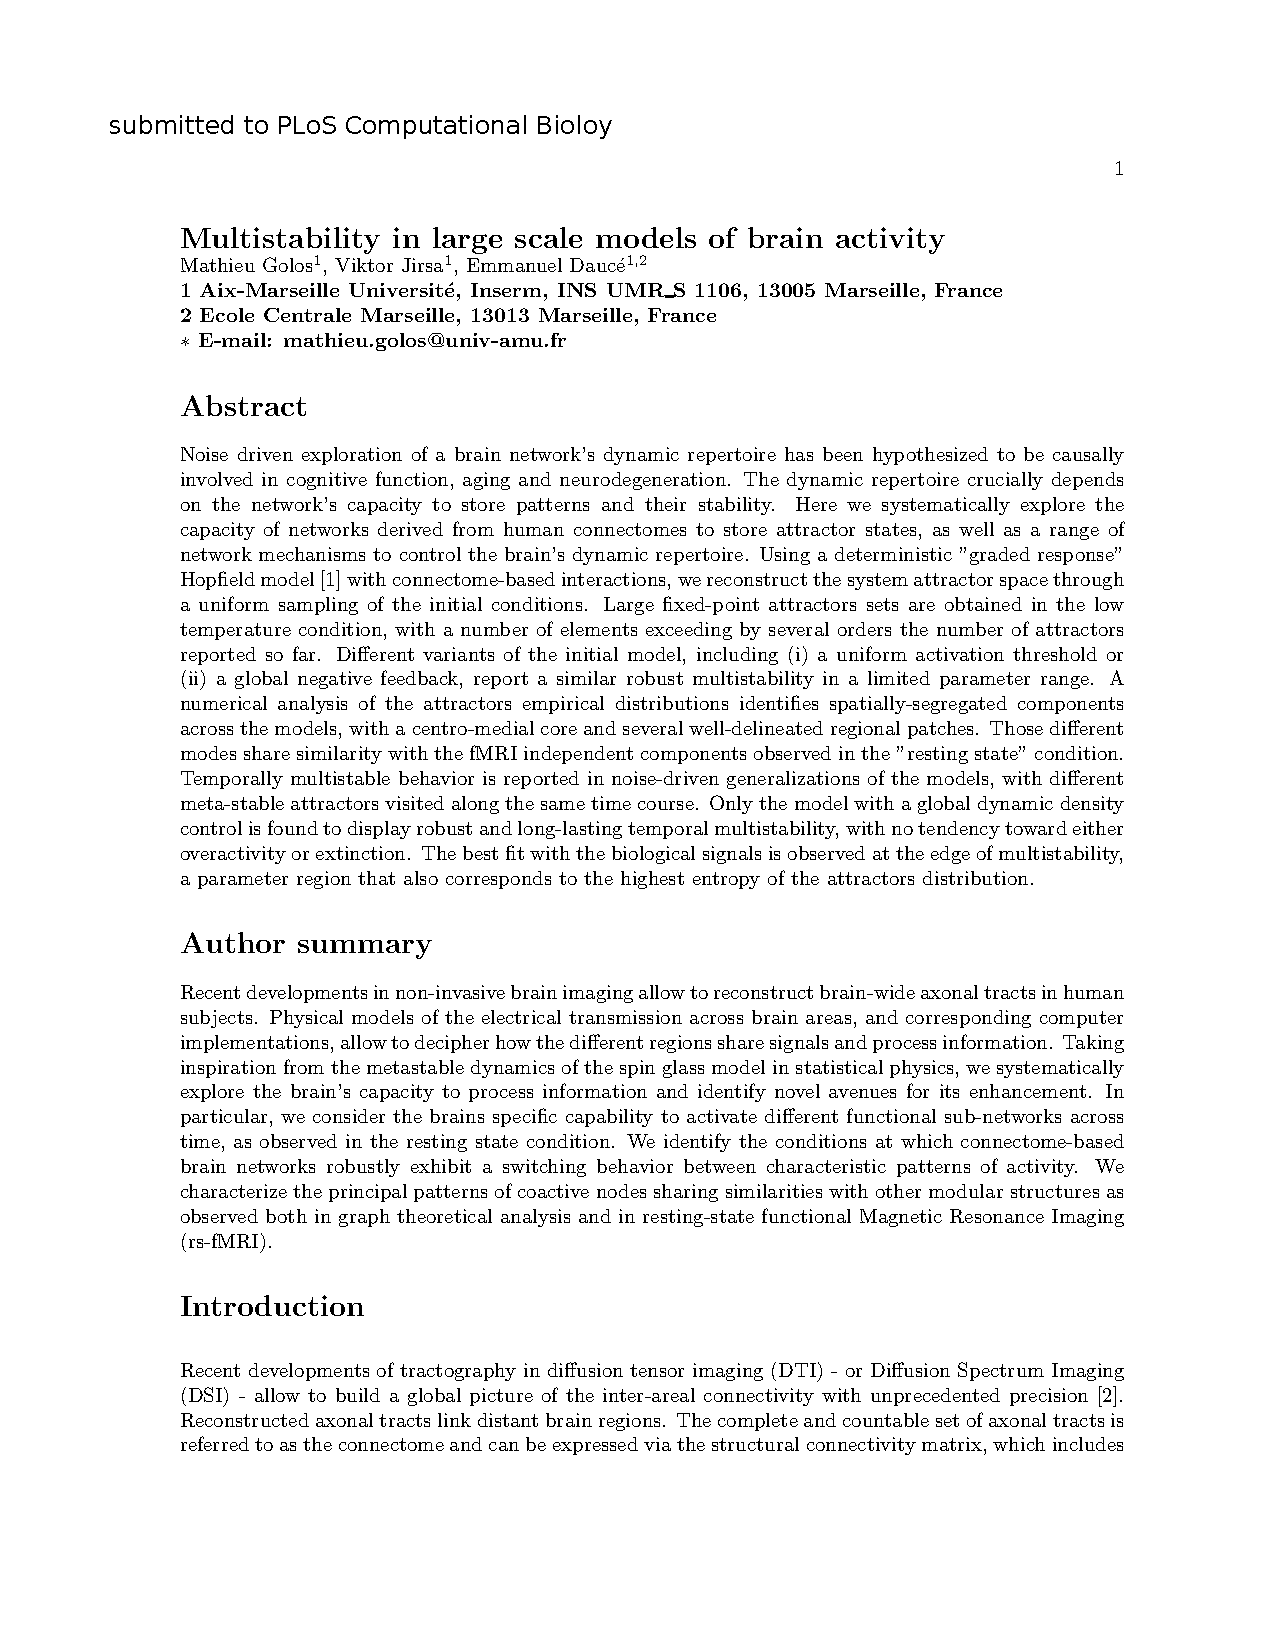
\includepdf[pages=1,offset=70 -20]{pdf/2015-PLOS-CB-ann.pdf}
%\includepdf[pages=2,offset=-70 -20]{pdf/2015-PLOS-CB-ann.pdf}
%\includepdf[pages=3,offset=70 -20]{pdf/2015-PLOS-CB-ann.pdf}
%\includepdf[pages=4,offset=-70 -20]{pdf/2015-PLOS-CB-ann.pdf}
%\includepdf[pages=5,offset=70 -20]{pdf/2015-PLOS-CB-ann.pdf}
%\includepdf[pages=6,offset=-70 -20]{pdf/2015-PLOS-CB-ann.pdf}
%\includepdf[pages=7,offset=70 -20]{pdf/2015-PLOS-CB-ann.pdf}
%\includepdf[pages=8,offset=-70 -20]{pdf/2015-PLOS-CB-ann.pdf}
%\includepdf[pages=9,offset=70 -20]{pdf/2015-PLOS-CB-ann.pdf}
%\includepdf[pages=10,offset=-70 -20]{pdf/2015-PLOS-CB-ann.pdf}
%\includepdf[pages=11,offset=70 -20]{pdf/2015-PLOS-CB-ann.pdf}
%\includepdf[pages=12,offset=-70 -20]{pdf/2015-PLOS-CB-ann.pdf}
%\includepdf[pages=13,offset=70 -20]{pdf/2015-PLOS-CB-ann.pdf}
%\includepdf[pages=14,offset=-70 -20]{pdf/2015-PLOS-CB-ann.pdf}
%\includepdf[pages=15,offset=70 -20]{pdf/2015-PLOS-CB-ann.pdf}
%\includepdf[pages=16,offset=-70 -20]{pdf/2015-PLOS-CB-ann.pdf}
%\includepdf[pages=17,offset=70 -20]{pdf/2015-PLOS-CB-ann.pdf}
%\includepdf[pages=18,offset=-70 -20]{pdf/2015-PLOS-CB-ann.pdf}
%\includepdf[pages=19,offset=70 -20]{pdf/2015-PLOS-CB-ann.pdf}
%\includepdf[pages=20,offset=-70 -20]{pdf/2015-PLOS-CB-ann.pdf}
%\includepdf[pages=21,offset=70 -20]{pdf/2015-PLOS-CB-ann.pdf}
%\includepdf[pages=22,offset=-70 -20]{pdf/2015-PLOS-CB-ann.pdf}
%\includepdf[pages=23,offset=70 -20]{pdf/2015-PLOS-CB-ann.pdf}
%\includepdf[pages=24,offset=-70 -20]{pdf/2015-PLOS-CB-ann.pdf}


\chapter{Plasticité synaptique et apprentissage}\label{chap:app}
Ce chapitre est consacré à l'étude des mécanismes d'apprentissage dans les réseaux de neurones récurrents.  


\textit{Ce chapitre présente une série de résultats regroupés sous le thème de la ``subjectivité perceptive''. Les modèles présentés
	explorent l'idée d'une autonomie partielle de la réponse logicielle à la commande. Vu sous l'angle neuromimétique, la 
	subjectivité perceptive consiste d'une part à ignorer certaines entrées sensorielles, du fait de leur non-pertinence ou de leur 
	non-conformité, et d'autre part à compléter certaines entrées sensorielles manquantes à l'aide de connaissances issues de l'expérience passée. 
	Nous regardons plus particulièrement la question de l'apprentissage, ou comment les règles de plasticité synaptique (le méta-programme) vont permettre à certaines
	stimulations sensorielles (désignées comme intéressantes) de ``creuser'' au sein du réseau un mode de réponse particulier (une ``résonance''),
	cette résonance étant le support des interpolations perceptives futures. Nous regardons également en quoi ces architectures dites ``à feedback positif'' 
	se distinguent du modèle classique du ``predictive coding'' organisé autour du principe du feedback négatif, et en particulier comment les premières
	implémentent le comportement de  ``résistance au changement'' (ou persévération). }


{\color{Cyan} Il est organisé en trois sections:
\begin{itemize}
	\item bla bla
	\item bla bla	
	\item bla bla
\end{itemize}
}

\section{Notions générales}

%\cleardoublepage

\subsection{Plasticité synaptique}

La synapse biologique est l'interface permettant la communication entre les neurones.
Il s'agit d'une petite surface d'échange chimique (``bouton'' synaptiques) située à l'extrémité de l'arborisation terminale des axones. A l'arrivée d'un potentiel d'action, les synapses libèrent des neurotransmetteurs qui agissent sur les canaux ioniques des dendrites de la cellule post-synaptique (``libèrent'' des ions), ce qui a pour effet de modifier le potentiel de membrane de la cellule post-synaptique.

L'efficacité d'une synapse dépend de plusieurs facteurs, comme la taille du bouton synaptique, la quantité de neurotransmetteurs disponibles,  ainsi que la sensibilité de la cellule post-synaptique. Dans le cadre de ce mémoire,  cet ensemble de facteurs est résumé  sous la forme d'une valeur unique $J_{ij}$ : le ``poids'' de la synapse, où  $j$ est l'index du neurone pré-synaptique et $i$ l'index du neurone post-synaptique.






{\color{Orange} Il existe, du point de vue biologique, des mécanismes de plasticité synaptique à court terme [REF STD] et à long terme [REF LTP]. On parle de potentiation à court terme vs. potentiation à long terme.}
Dans le cadre de ce mémoire, on considérera l'évolution des poids synaptiques comme ``lente'' par rapport à la dynamique d'activation (autrement dit que les poids synaptiques sont quasi-stationnaires sur de petits intervalles de temps).

Cette dynamique lente a un impact sur le comportement du réseau de neurones sur le long terme. Il s'agit essentiellement, selon l'idée initiale de Hebb, d'un mécanisme 
de sélection dans lequel des activités corrélées tendent à se connecter, et des activité décorrélées à se déconnecter. 
La règle de Hebb s'interprète donc généralement comme une règle qui inscrit dans le graphe la structure de covariance présente dans l'activité des neurones. Lorsque l'activité est elle-même induite par le signal d'entrée, le graphe reflète en partie les covariances présentes dans le signal.

{\color{Cyan}
Exemples (avec maths):
\begin{itemize}
	\item Co-activité
	\item Covariance
	\item STDP
\end{itemize}
}

\paragraph{STDP}

% % Plasticité de Hebb


\subsection{Apprentissage}

\subsubsection{Perspective biologique}
Selon une perspective biologique et développementale, l'apprentissage
est le processus de changement comportemental, 
en relation avec ce mécanisme de plasticité. 
L'apprentissage est au sens large
l'ensemble des processus épigénétiques (historiques) inscrivant dans l'animal ou l'individu 
les éléments d'expérience qui contribuent à accroître l'adaptation de ses réponses à son
milieu.  

Cette capacité à inscrire des événements ou des faits particuliers en vue de les exploiter dans le futur est une des
propriétés essentielle du système nerveux des être vivants. 
Mieux comprendre les mécanismes biologiques qui sous-tendent cet apprentissage est un des défis majeurs pour les neurosciences computationnelles. Si la plasticité synaptique semble être le principe explicatif majeur de l'apprentissage, il reste encore de nombreuses zones d'ombre 
\begin{itemize}
	\item sur les caractéristiques précises de cette plasticité;
	\item sur les mécanismes de choix qui vont sélectionner certains signaux et certains événements plus significatifs;
	\item sur les déterminants macroscopiques des changements microscopiques et vice-versa.
\end{itemize}





%{\color{Gray} Ce qui différencie principalement le calcul traditionnel du calcul distribué est la taille et la dimension des opérandes. Le calcul distribué s'adapte bien à la réalisation d'opérateurs (a priori non linéaires) dans les espaces de grande dimension. }




{\color{Cyan} Remarque~: projection dans un espace de pls grande dimension \--- espace de redescription.}

{\color{Cyan} 
	Exemples :
	\begin{itemize}
		\item Appariement sélectif~: les barycentres des partitions génératrices permettant d'interpréter une donnée d'entrée comme membre d'une classe donnée. Principe de l'argmax ou du ``winner takes all''. Non-linéaire. Mécanisme de \emph{choix}. \textit{Enumeration.}
		\item Appariement non sélectif : les données sont interprétées comme une combinaison de facteurs.  projection des données sur une base de plus petite dimension. Matching pursuit. Dictionnaire. Combinaison linéaire. ACP, SVD, deep learning, ... \textit {Décomposition}.
	\end{itemize}
}

\paragraph{Types de données}

La construction du dictionnaire de formes s'appuie sur des contraintes exprimées dans les données d'apprentissage. On distingue en général l'apprentissage guidé par l'erreur (supervisé ou semi-supervisé) et l'apprentissage guidé par le modèle.
\begin{itemize}
	\item L'apprentissage est guidé par l'erreur lorsqu'il existe une fonction d'erreur (ou fonction de ``\textit{feedback}'') $l$  qui ``note'' la réponse produite par la fonction de réponse. Exemples~:
	\begin{itemize}
		\item  fonction différence~: $l(y,f_T(x)) = y - f_T(x)$
		\item fonction distance~:
		$l(y,f_T(x)) = ||y - f_T(x)||$
		\item fonction de perte (ou  ``\textit{loss}'')
		$l(y,f_T(x)) = \mathbf{1}_{y \neq f_T(x)}$
		\item etc...
	\end{itemize}
	Le guidage est plus ou moins contraignant selon le type de fonction d'erreur considéré. 
	\begin{itemize}
		\item On parle d'apprentissage \textit{supervisé} (ou à information totale) lorsque la réponse désirée est connue,
		\item et d'apprentissage \textit{par renforcement} (ou à information partielle) lorsque la fonction d'erreur ne fournit qu'une ``indication'' (de type ``bien/mal) sur la justesse de la réponse.  
	\end{itemize} 
	\item L'apprentissage est guidé par le modèle lorsque les capacités d'expression de la fonction de réponse (principalement le nombre et le type de formes \---~ou classes~\--- identifiables) contraignent l'espace des réponses possibles. On parle d'apprentissage \textit{non supervisé}.
\end{itemize}
Le principe d'un guidage plus ou moins contraignant se retrouve également dans la littérature de psychologie expérimentale classique, dans laquelle on parle~:
\begin{itemize}
	\item de conditionnement pavlovien (lorsque le comportement est guidé par une réponse réflexe à un stimulus) {\color{Cyan}[PAVLOV]}
	\item et conditionnement opérant (lorsque le comportement est guidé par une récompense ou une punition) {\color{Cyan}[SKINNER]}. 
\end{itemize} 



{\color{Orange} Hypothèse du sampling en neurosciences.}

\paragraph{Apprendre et oublier}

Une dernière distinction concerne le caractère stationnaire ou non-stationnaire des données d'apprentissage lorsque le jeu de données est indexé sur l'axe temporel. 

On parle d'apprentissage ``en ligne'' lorsque les données sont présentées séquentiellement.
L'apprentissage consiste à appliquer de petits ajustements à chaque nouvelle donnée dans un 
sens qui augmente localement la justesse de la fonction de réponse, en espérant que chacun de ces ajustements locaux 
augmente la justesse globale,
selon le principe de la descente de gradient ``stochastique''.

Ce mécanisme d'apprentissage en ligne a l'avantage de rester valide lorsque les données sont non-stationnaires Ainsi les régularités observées durant les premières phases de l’apprentissage ne sont plus nécessairement présentes
à une étape ultérieure de l'apprentissage.
%~: certaines trajectoires sont ``abandonnées''. 
Dans une perspective de parcimonie 
(ou de ressource limitée), il est avantageux d'oublier certains faits passés pour mieux appréhender les faits nouveaux, autrement
dit oublier pour mieux apprendre.
Cette prise en compte du ``vieillissement'' de l'environnement conduit à accorder plus de crédit à des observations
récentes qu'aux observations anciennes \shortcite{Kivinen2004}, et donc \textit{oublier pour mieux apprendre}. 


%{\color{Cyan}
%\subsubsection{Perspective psychologique}
%Le conditionnement Pavlovien.

%L'approche constructiviste (Piaget).
%}



{\color{Gray}Hebb a été influence par la psychologie expérimentale de son époque et transpose les principes du conditionnement opérant au cadre microscopique.   }

%Dans une perspective computationnelle, si la fonction d'activation $f$ définit le programme, la fonction de mise à jour des poids $F$ agit sur le programme implémenté par $f$. La fonction $F$ peut donc être vue comme un mécanisme de programmation du calculateur $f$. 

%Approche empirique: reproduire l'apprentissage via la plasticité sur un support artificiel.

%en modifiant son activité, sa réactivité à certaines entrées, ou le type de
%réponse qu'il produit. 


{\color{Orange} Le but est d'implémenter via la plasticité une mémoire ``persistante'', qui provoque un changement durable de la fonction de réponse.
	On souhaite inscrire sur
	le graphe de connexions la trace de faits passés en vue d'une utilisation future.}

%{\bf !!Plaçons-nous par exemple dans une perspective computationnelle autonome!!}, 
%dans laquelle un programme doit pouvoir se passer d'utilisateur. 
%La consigne doit provenir d'un programme interne (un ``méta programme'') qui 
%agit sur le programme courant pour l'``améliorer'' en fonction des événements se présentent.
%{\bf !!Même si la notion de méta-programme ne pose pas de difficulté conceptuelle, elle est
%	en pratique difficile à mettre en oeuvre dans les architectures informatiques traditionnelles. 
%	La difficulté réside dans 
%	le choix des événements à considérer parmi l'ensemble des événements qui se présentent, et surtout 
%	dans la manière dont les événements pris en compte influencent le comportement logiciel futur.}

%Il existe deux grandes approches de la plasticité~:
%\begin{itemize}
%	\item Apprentissage sans consigne.
%	\item Apprentissage avec consigne
%\end{itemize}

%\cleardoublepage



\section{Notions spécifiques et propositions}

Cette section présente quelques notions plus spécialisées utiles à la compréhension de mes travaux, dédiées à l'étude de la plasticité des réseaux de neurones récurrents. 

{\color{Gray} Ne prenant pas en compte de signal d'erreur, cette règle est classiquement interprétée dans le cadre 
théorique de l'apprentissage non-supervisé. 
2 principes d'apprentissage connus semblet liés à la règle de Hebb:
\begin{itemize}
	\item l'auto-encodage (au sens Kohonen mais pas au sens deep)
	\item l'apprentissage associatif (modèle de Hopfield) 
\end{itemize}
Ces modèles sont porteurs de limitations (en terme de capacité de stockage ou de preuve de convergence) qui rendent difficiles l'utilisation de la règle de Hebb dans le cadre de problèmes pratiques. }


{\color{Cyan}
	Idée de base~: étudier le rôle de l'activité récurrente (persistante) dans le cadre de l'apprentissage. En particulier: reconnaissance de patrons spatio-temporels. 
	
	Mécanisme d'appariement distribué: l'opérateur est l'opérande et subit les transformations.   
	
	Le modèle qui est proposé, c'est principalement une alternance entre (i) absence de réponse et (ii) mise en œuvre de programmes moteurs spécifiques.
	
	Ce fonctionnement est lié au principe d'assemblée neuronale et à la plasticité de Hebb, à travers la notion  de sélection (au sein d'un réservoir).
	
	On peut étendre à l'idée de vocabulaire comportemental/appariement sélectif/''winner takes all''/argmax.
	
	Modèle de mémoire basé sur l'interprétation suivante ~: les formes mémorisées sont des ``faits''. 
	
	
	PROPOSITIONS :
	
	
	
	{\bf 
		
		
		
	\begin{itemize}
		\item  
		\item 
		\item 
		
		\item La convergence vers l'attracteur n'étant pas immédiate, .
	\end{itemize}
	}
	
%	{\color{Red} IL FAUT CREUSER ET DEVELOPPER CETTE NOTION D'APPARIEMENT}

	
	}
	




\paragraph{Cas des réseaux de neurones récurrents} 
\subsection{Mise en œuvre et applications}

\subsubsection{Intégration}

Contrairement aux modèles classiques dans lesquels l'appariement 
repose sur un produit scalaire, l’appariement s'effectue dans les réseaux récurrents via  mécanisme de relaxation vers un attracteur.

Le calcul de la réponse (le patron d'activité final) repose sur la stabilisation progressive d'un circuit d'activation particulier, les valeurs calculées aux temps précédents étant réutilisées  pour aboutir progressivement au patron d'activité final. On parle dans ce cas de processus  d'\textit{intégration} de la réponse (au sens de l'intégration progressive au cours du temps de caractéristiques d'activation conduisant au patron final).
 
Il n'y a donc pas, dans ce cadre, de distinction entre opérateur et opérande. L'information ne circulant pas dans un sens défini (de l'entrée vers la sortie), l'activité d'un nœud est, selon l'avancement du processus d'intégration, un opérande (une entrée) ou le résultat d'une opération.

Le résultat macroscopique de ce processus est un mécanisme d'\textit{accroissement d'évidence}, inscrit dans le temps, conduisant 
au ``choix'' d'une des formes préalablement stockées dans le réseau. 

Le modèle de Hopfield 
est un exemple d'implémentation de ce mécanisme d'appariement entre un signal d'entrée, 
fourni sous forme de condition initiale, et un des patrons stockés dans le graphe.
{\color{Orange} Il s'agit également une optimisation sous contraintes. Les liens sont les contraintes, il existe un terme d'énergie, avec convergence vers une solution locale (trouver ref dans bouquin ``dynamique des syst. complexes''+ à mettre en lien avec Berrou).}

\subsubsection{Filtrage}\label{sec:filtrage}

Selon les modèles classiques, la perception sensorielle s'apparente à un mécanisme de \textit{filtrage} des entrées perceptives.
Le filtrage d'un signal correspond fonctionnellement au fait de pouvoir \textit{prédire le présent}. 
Tout écart entre la prédiction et l'observation constitue un erreur de prédiction.
La perception sensorielle est interprétée comme le résultat de l'intégration des erreurs perceptives afin de mettre à jour le modèle. 

Le filtrage repose sur un \textit{modèle} prédictif (ou modèle interne)
%Il nécessite également le maintien d'une activité prédictive interne
généralement implémenté  %un modèle ``forward'' permettant d'appliquer 
selon le principe de l'``observateur''
\cite{Kalman1960,Wolpert2000}, où:
\begin{itemize}
	\item La sortie du modèle correspond à la prédiction actuelle,
	\item Le signal d'entrée correspond
	à l'observation effective. 
\end{itemize}

%\begin{itemize}
%	\item se manifeste par la présence d'une erreur perceptive 
%	\item et se résout via un mécanisme de traitement de l'erreur.
%\end{itemize}

La présence d'une erreur sensorielle fait entrer le système dans un conflit qui peut se résoudre de deux manières~:
\begin{itemize}
	\item Les modèles de la perception basés sur un appariement négatif \shortcite{Rao1999,Friston2009} font disparaître de la scène sensorielle les
	éléments prédits, de sorte que, selon cette théorie, 
	ce qui est ``perçu'' (ou intégré) est l'erreur sensorielle,
	autrement dit la différence entre sensation et la prédiction.
	\item Les modèles de la perception basés sur un appariement positif ``complètent'' le signal d'entrée avec le signal prédit:
	\begin{itemize}
		\item Si l'écart est faible, le système tend à ignorer ce changement
		et persévère dans sa prédiction.
		\item Si l'écart est important et/ou réitéré, le système met
		à jour (reconfigure) son activité interne (son ``modèle'') afin de mieux anticiper l'entrée.  
		\end{itemize} 	
\end{itemize}

{\color{Gray} D'un point de vue computationnel, le feedback sensoriel positif fonctionne selon un principe de ``pattern matching'',
qui s'oppose dans son principe aux mécanismes de correction d'erreur basés sur le feedback négatif (``pattern mismatch'').}

La persévération présente de nombreuses analogies avec les mécanismes de mémoire à court terme 
{\color{Orange} décrits précédemment}. 
Si une partie du signal disparaît par exemple, l'activité interne est 
capable de compléter les morceaux manquants, selon un mécanisme auto-associatif qui s'apparente
à celui des réseaux de Hopfield. Le réseau peut continuer par exemple à ``croire'' à l'intégrité des éléments de la scène visuelle
(sensorielle) non perçus à cause de phénomènes d'occlusion.

Chacune des approches présente des avantages et des inconvénients. 
\begin{itemize}
	\item L'appariement positif apporte de la robustesse, de la
	mémoire à court terme (complétion, interpolation des données manquantes, traitement des ambiguïtés perceptives) 
	mais peut également produire une résistance excessive aux changements
	de la scène sensorielle. Le cas limite correspond au réseau qui ignore totalement son entrée sensorielle, 
	persévérant indéfiniment sur un illusion perceptive produite par l'activité interne (``hallucination'').
	\item L'appariement négatif apporte une parcimonie (perception de la différence d'activité), qui permet d'implémenter 
	un principe de ``matching pursuit'' pour un traitement rapide du flux visuel \shortcite{Perrinet2010}.
	Il présente cependant une sensibilité au bruit de mesure (fluctuations aléatoire), 
	{\color{Orange} et nécessite dans certains cas la mise en place d'une remise à zéro 
	périodique , qui peut être réalisée par une alternance entre mesure de l'erreur (perception) et correction 
	d'erreur (déplacement moteur).} 
\end{itemize}

%dans le cas de signaux spatio-temporels\footnote{Sauf si, évidemment, le modèle forward est fourni,
%auquel cas .




\subsection{Le principe du réservoir}



Complexité, chaos et réduction de la complexité.


%\subsection{Principe d'appariement sélectif}





%finissent la manière dont les données vont être traitées et interprétées.


\subsection{Sélection/intégration}

Mécanismes de choix qui sélectionne les signaux et les événements plus significatifs;

Passage de seuil. ``Spike'' de population. De la cellule à la population. 
Réponse de population induite.

(Freeman) et  sélection/intégration  par réduction

Calcul collectif - intégration - assemblée

Mecanisme de choix. Lien entre choix et plasticité. On reconnait ce que l'on connait (Reconnaisance et connaissance). analogie avec spike de population (spike = significatif) 



sélection = Analogie accumulation d'évidence?

\subsection{Construire les modes de la fonction de réponse}

Une des thèses du mémoire : feed+/feed-.

%\cleardoublepage

\section{Contributions personnelles}

{\color{Cyan}
	Par rapport aux propositions, j'ai fait:
	\begin{itemize}
		\item ceci
		\item cela
		\item etc.
	\end{itemize}
}	

\subsection{Route inverse}\label{sec:NN98}

L'étude du mécanisme de reconnaissance par ``réduction'' de la dynamique constitue le cœur
de ma thèse, sous la direction
de Bernard Doyon, chercheur à L'INSERM au sein de l'équipe dirigée par Manuel Samuelidès à l'ONERA 
de Toulouse, entre 1996 et 1999. 
Certains travaux réalisés pendant la thèse de Mathias Quoy (1991-1994) \shortcite{Quo94}
avaient déjà montré l'effet de réduction produit par 
la plasticité Hebbienne dans les réseaux aléatoire récurrents à 
dynamique chaotique intrinsèque.

Le papier qui présente ces idées de la manière la plus complète est celui de Neural Networks, 
datant de 1998 \shortcite{Dau98A}.
Il porte sur l'étude de la réaction (spontanée ou acquise) d'un réseau de neurones récurrent aléatoire
à des patrons (stimuli) également aléatoires.
Il fait la synthèse de plusieurs résultats sur les réseaux récurrents aléatoires, 
à la fois sur les comportements de grande taille et 
sur les effets de taille finie, et présente pour la première fois les effets de la plasticité sur ce type de réseau.
Il reprend pour ce qui me concerne des travaux réalisés pendant ma première année de thèse. %DAU98B}. 
Les réseaux étudiés étant normalisés, 
leur comportement est réglé par deux paramètres~: le gain de la fonction de réponse neuronale (assimilable
à l'inverse d'une température) et la variabilité du seuil d'activation.
Le signal présenté en entrée du réseau est un patron aléatoire statique qui vient se surimposer au seuil 
d'activation (rendant donc les neurones plus ou moins excitables).
Le réseau soumis à un tel signal converge vers un nouvel attracteur (autrement dit se reconfigure).

\begin{figure}[b!]
	\centerline{
		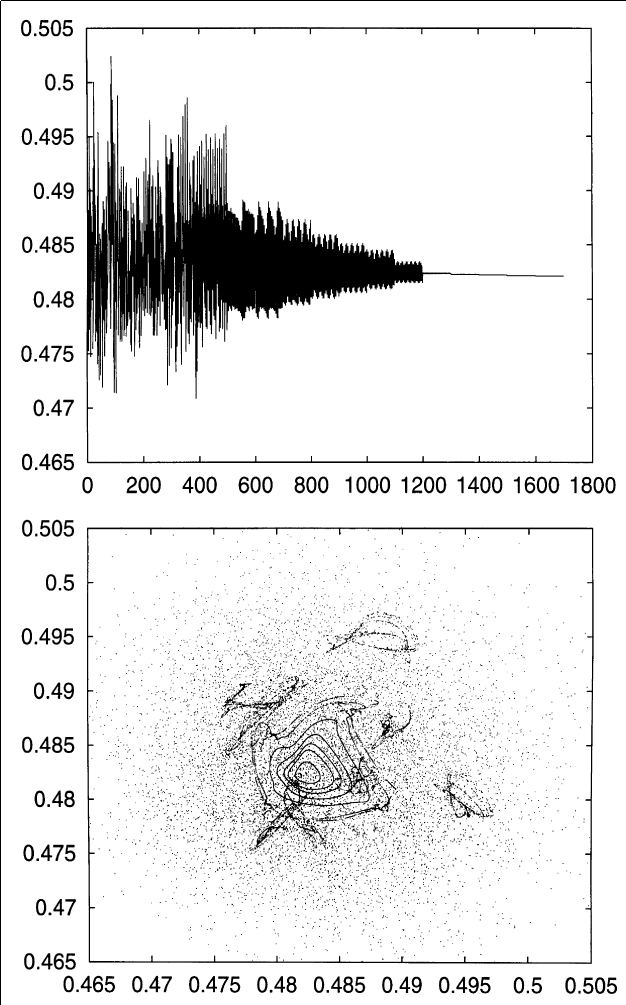
\includegraphics[width = 0.5\linewidth]{figs/NN98-inverse.png}
	}
	\caption{\footnotesize{(A) Evolution of the stimulus-forced average activity $m_\text{net}(t)$ versus time $t$
			during the learning process. There is one learning step every 100 time step.
			In that example the dynamics is reduced to a fixed point after 12 learning
			steps ($t = 1200$). (B) Representation of the corresponding attractors in the
			$[m_\text{net}(t), m_\text{net} (t+1)]$ phase plane. Note the decrease of the diameter of the limit
			cycles at each learning step (From Daucé et al., 1998)}.}
	\label{fig:inverse}
\end{figure} 

{\color{Gray} Le point important est que le réseau ne produit pas de réponse (de ``read out'').
	Le changement d'activité induit par la surimposition du patron statique n'a pas de signification
	particulière. Il est juste possible, du point de vue extérieur, 
	de distinguer la nouvelle organisation de l'ancienne, à partir de 
	différents observables (indice de complexité, période interne, répartition des niveaux d'activité).}

Le changement observé suite à la présentation d'un stimulus statique ne correspond pas à 
de la multistabilité au sens classique (un système dynamique multistable pouvant converger 
vers différents attracteurs pour des conditions initiales différentes).
Ici le stimulus fait partie des ``paramètres'' du
réseau. Ainsi, chaque stimulus distinct définit système dynamique distinct 
convergeant vers un attracteur distinct. 
Le fait de modifier le stimulus au cours d'une même simulation 
revient à modifier le système dynamique ``en cours de route''. 
La réalisation d'une opération (sous la forme d'une réorganisation de la dynamique
suite à l'imposition d'un motif statique) repose
donc sur un mécanisme différent de celui proposé par Hopfield~:
\begin{itemize}
	\item
Il s'agit essentiellement d'une relaxation sous contrainte, chaque
stimulus étant l'expression d'une contrainte différente.
\item
L'ensemble des réponses aux contraintes statiques possibles constitue le \textit{répertoire 
	dynamique} du réseau.
\end{itemize}

Une règle de plasticité synaptique est ajoutée, correspondant à un dynamique lente sur les couplages, qui modifie 
le graphe selon une règle inspirée de Hebb \shortcite{Heb49}~:
$${J}_{ij}(t) - {J}_{ij}(t-1) \propto (s_i^\text{out}(t)-0.5)\times(s_j^\text{in}(t)-0.5)$$
(à savoir que le lien entre deux neurones se renforce s'il
existe une corrélation entre l'activité pré-synaptique et l'activité post-synaptique).
Le papier étudie les changements dans le répertoire dynamique lorsque le réseau est soumis à ces changements 
synaptiques dans le contexte d'une contrainte statique spécifique.  
Le papier met en évidence des changements de comportements liés à cette dynamique sur les poids, conduisant 
systématiquement à une simplification de l'activité intrinsèque (par exemple passage d'une activité
chaotique à une activité de type cycle limite). On parle de ``réduction'' de la dynamique, la plasticité 
produisant une ``route inverse'' de la complexité vers le point fixe
(voir figure \ref{fig:inverse}).

Une fois la session d'apprentissage terminée, la présentation du stimulus appris 
a pour effet d'induire cette dynamique moins complexe (obtenue en fin de session).
Cette activité est qualitativement différente, plus simple que l'activité induite par les autres stimuli. 
La plasticité permet donc d'obtenir une réaction spécifique à une entrée particulière (ici une
forme arbitraire générée par un tirage aléatoire). 

La plasticité Hebbienne a donc pour effet de créer des comportements ``acquis'' spécifiques.
Le mécanisme de Hebb (renforcement des liens entre les neurones les plus actifs) 
tend à produire une classe de réactions différente
face aux motifs appris. Les motifs en question sont ``reconnus''. 
Le reste des motifs,
ne présentant pas ces caractéristiques spatiales spécifiques, induisent une réaction ``par défaut''
qualitativement différente.
Il y a donc, pour des motifs quantitativement similaires (issus d'un tirage aléatoire de même loi), 
des réponses qualitativement différentes.
Ce mécanisme de séparation entre le connu et l'inconnu
(appariement conditionnel) 
%par le comportement dynamique du substrat
rejoint l'hypothèse formulée par Freeman \shortcite{ska87} à propos de la perception des odeurs~: 
activité simplifiée pour des odeurs connues, activité de fond chaotique pour les odeurs non familières.

%Du point de vue computationnel, la plasticité synaptique indit une séparation de l'espace
%des stimuli entre une région reconnue et une région inconnue. Il s'agit donc en premier lieu d'une opération de 
%discrimination. Deuxièmement, c
Chaque réponse à un motif se traduit par une activité spatio-temporellement distincte,
l'apprentissage ayant pour effet de capturer (ou plutôt accentuer) un \emph{mode dynamique} particulier.
Le réseau est vu comme un ``réservoir'' de comportements dynamiques spatio-temporellement différents. Le comportement
spatio-temporel asocié au motif change sous l'effet de la plasticité, en conservant certaines
de ses caractéristiques comme la période intrinsèque, qui se manifeste de façon ``pure'' 
sous la forme d'un cycle limite. Ce comportement temporellement périodique 
finit par disparaître si l'apprentissage est poussé jusqu'au point fixe. La règle 
de plasticité Hebbienne, dans sa forme simple étudiée ici, n'est pas convergente et 
l'apprentissage est stoppé de manière arbitraire à l'apparition du cycle limite
pour les besoins de l'étude. 

La principale difficulté rencontrée pour ces réseaux est la contamination 
de la réaction induite à des patrons non appris. Si des motifs voisins du motif initialement appris
induisent également une réduction de la dynamique, la réitération de l'apprentissage sur plusieurs motifs différents
conduit invariablement à un effondrement généralisé de la complexité, étendant la réduction de
dynamique à l'ensemble des motifs. 
La capacité d'un réseau est définie comme le nombre de motifs pouvant être 
appris sans provoquer cet effondrement.
Cette capacité s'avère assez faible en pratique. 
Dans notre cas, comme dans le cas du réseau de Hopfield, elle semble
dépendre linéairement de la taille du réseau.

Des changements marginaux sur la règle de plasticité, en limitant drastiquement le nombre
de liens éligibles,
permettent d'augmenter significativement la capacité des réseaux \shortcite{Dau98B,Dau98C},
avec une 'loading capacity' empirique de l'ordre de 8\% (le nombre de
motifs pouvant être appris avant l'effondrement catastrophique est de l'ordre de
8 \% du nombre de neurones, ce qui reste relativement faible).

%{\color{Violet}

%Impact du papier?

Le papier de Neural Networks, en démontrant pour la première fois l'effet de la plasticité Hebbienne sur 
la dynamique intrinsèque des réseaux récurrents aléatoires, a reçu une bonne audience, dans la mesure où il est 
un des premiers à présenter un cadre mathématique pour l'étude des réseaux de neurones récurrents perturbés
par un signal extérieur. Le même principe est utilisé, dans une certaine mesure, dans les modèles de contrôle 
proposés par Jun Tani dans les années 90 \cite{Tani2004}, ainsi que dans les modèles de réservoir computing proposés par 
Maas et Markram \cite{MAASS02,Buonomano2009}.



%\shortcite{Dau98A} {\bf Daucé, E., Quoy, M., Cessac, B., Doyon, B. and Samuelides, M. (1998) Self-organization and dynamics reduction in recurrent networks : stimulus presentation and learning, Neural Network 11:521-533}

%\shortcite{Dau98B} {\bf Daucé E. and Doyon, B. (1998) Novelty Learning in a Discrete Time Chaotic Network, proc. of the 8th International Conference on Artificial Neural Networks (ICANN'98), L. Niklasson et al. eds, Vol. 2: 1051-1056, Springer, September 2-4, Skövde, Sweden}



%- Une méthode d’apprentissage “non-supervisée” (il s’agit de capturer un mode dynamique)

%- mecanisme de base de la route inverse. Notion de “reduction” de la dynamique par apprentissage (baisse de l’impredictibilité, analogie possible avec exploration/exploitation)

%- encodage - patrons statiques - route vers le chaos - destabilisation - frontière du chaos
%}

%\cleardoublepage

\subsection{Architectures multi-couches} \label{sec:BioCyb02}


Les travaux présentés dans \shortcite{Dau00,Dau02} présentent une architecture 
neuronale  permettant d'implémenter un modèle de la perception des signaux spatio-temporels.
Ils reposent sur une architecture de réseaux récurrents aléatoires à plusieurs couches (deux ou trois).
Le formalisme multi-couches est le même que celui utilisé dans les réseaux équilibrés (voir section \ref{sec:balanced}).
Ici les couches se distinguent non par la nature de leurs neurones mais par le rôle qu'elles prennent dans le processus
d'apprentissage~: 
\begin{itemize}
	\item une (ou deux) couche(s) primaire(s) ayant un rôle passif (sans dynamique intrinsèque)
\item et une couche secondaire (ou associative) possédant une dynamique intrinsèque, analogue aux réseaux récurrents aléatoires
simples présentés dans la section \ref{sec:NN98}.
\end{itemize}

Le modèle se présente comme une architecture générique pour l'apprentissage 
de motifs spatio-temporels (voir figure \ref{fig:BC02-archi}). 
{\color{Orange} Comme dans le cas précédent, il ne s'agit pas de l'apprentissage d'une réponse 
(d'un read-out) mais d'une modification du comportement du système dynamique en présence
de certains signaux.} La contrainte extérieure se manifeste ici sous
la forme d'un signal spatio-temporel périodique, et la relaxation s'apparente à celle d'un oscillateur
forcé. 
Dans cette étude, comme dans l'étude précédente, l'accent est mis sur la plasticité et l'apprentissage, où 
le comportement ``différent'' est un comportement acquis. 

\begin{figure}[b!]
	\centering
	{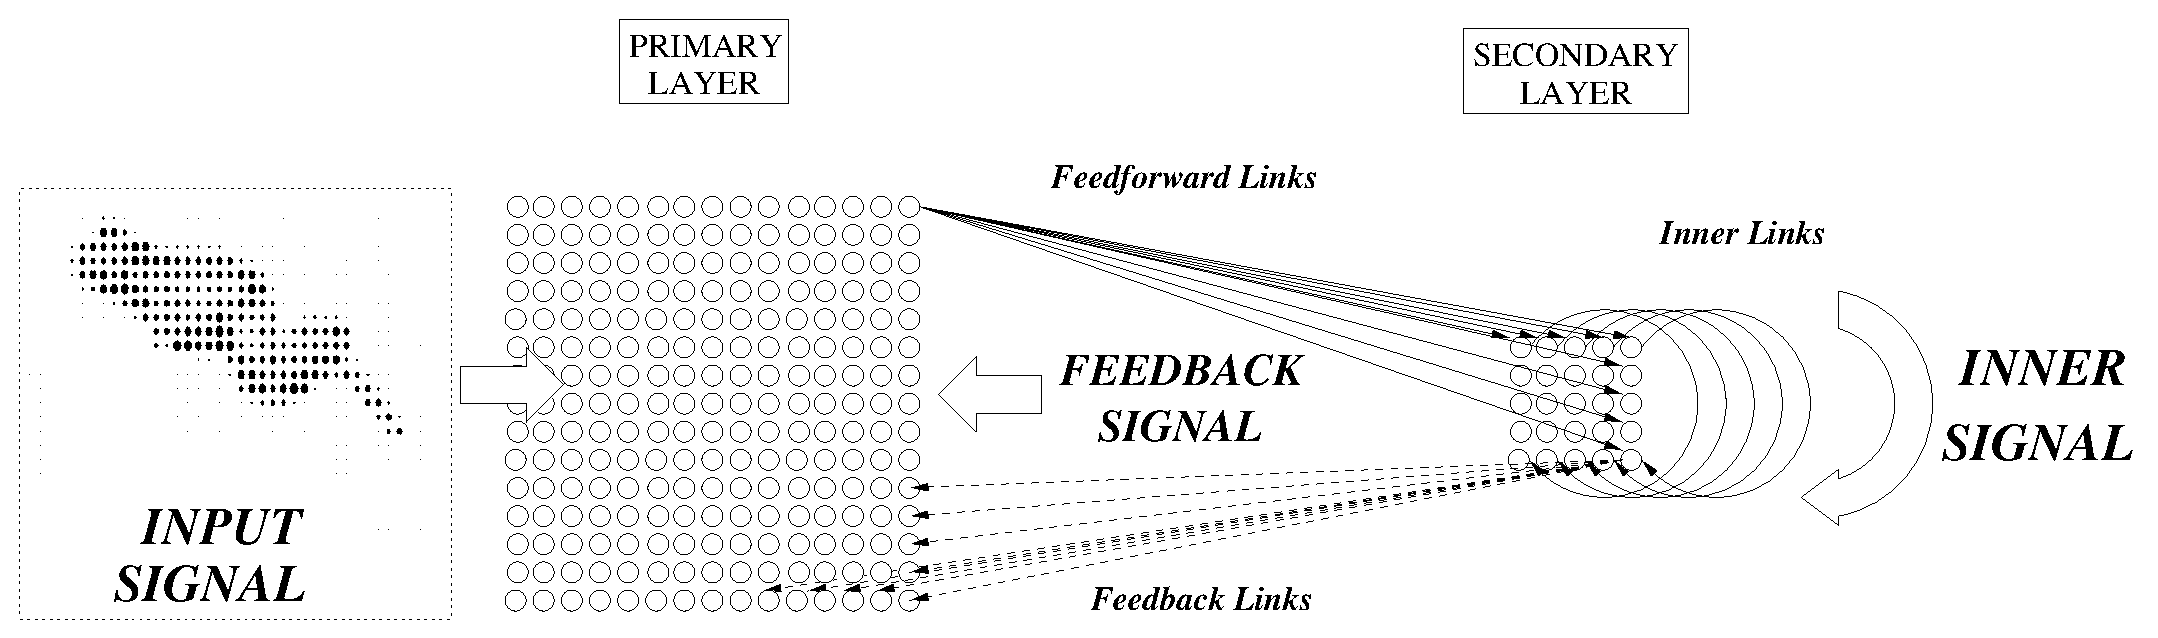
\includegraphics[width=\linewidth]{figs/bc_archi.eps}}
	\caption{\footnotesize{{\bf Architecture of the ReST model}.
			Our model is composed of two layers. Their respective sizes are
			not necessarily equal. Only few links are represented. The primary
			layer is submitted to a spatio-temporal input pattern. 
			The secondary layer has no input signal. The
			links are monodirectional. The activity of the secondary layer (inner
			signal) is chaotic. The activity on the primary layer depends both on
			the input signal and feedback signal from the secondary layer (from Daucé et al, 2002).} }
	\label{fig:BC02-archi}
\end{figure}

La règle Hebbienne utilisée est une règle d'ordre 1 (basée sur les différences d'activité), qui
modifie les couplages synaptiques selon une estimation locale de la covariance entre les neurones 
pré et post-synaptiques, en tenant compte du délai de transmission \shortcite{Sej77}. 

$${J}_{ij}(t) - {J}_{ij}(t-1) \propto (s_i^\text{out}(t)-m_i^\text{out}(t))\times(s_j^\text{in}(t)-m_j^\text{in}(t))$$
avec~:
$$m_i(t) = \beta s_i(t) + (1 - \beta) m_i(t-1) \text{, avec } \beta \in ]0,1[ $$

Cette règle, contrairement à la précédente, 
tend à amplifier les variations d'activité. Elle tend asymptotiquement
vers une activité de type cycle limite très robuste à large amplitude individuelle (et non vers un point fixe).
Comme dans le cas précédent, du fait de la non-convergence asymptotique,
la durée d'apprentissage est fixée par l'utilisateur/concepteur
en vue d'optimiser un certain comportement (ici la résonance perceptive). 

Dans la configuration initiale, la couche primaire reçoit passivement le signal spatio-temporel (séquence 
périodique de motifs). Les liens feed-forward aléatoires transmettent ce signal à la couche 
secondaire (dite couche associative). L'activité de la couche associative est un mélange entre cette projection aléatoire
du signal d'entrée et l'activité intrinsèque chaotique (entretenue par les liens latéraux
aléatoires de la couche secondaire). Les liens de feedback (secondaire vers primaire) sont initialement nuls.



La plasticité synaptique a lieu sur deux classes de liens~: latéraux et feedback.  
{\color{Gray} Elle inscrit dans le graphe les 
séquences d'activation prédictibles au sein de l'activité neuronale. }
Outre la réduction de la complexité de l'activité,
la plasticité des liens de feedback crée une boucle d'amplification positive entre la couche associative
et la couche sensorielle, qui transforme la corrélation statistique 
en lien de causalité (voir figure \ref{fig:BC02-app}).
\begin{itemize}
\item L'existence de correspondances statistiques entre l'activité interne et le signal d'entrée produit en effet une amplification du signal d'entrée via cette activité de feedback.
\item Cette projection induite de l'activité interne vers la couche sensorielle
agit comme une prédiction \textit{dans le présent} (voir section \ref{sec:filtrage}), autrement dit fait reposer la connaissance de l'entrée
sensorielle actuelle sur des informations observées dans le passé.
\end{itemize}

\begin{figure}[p]
\centering{
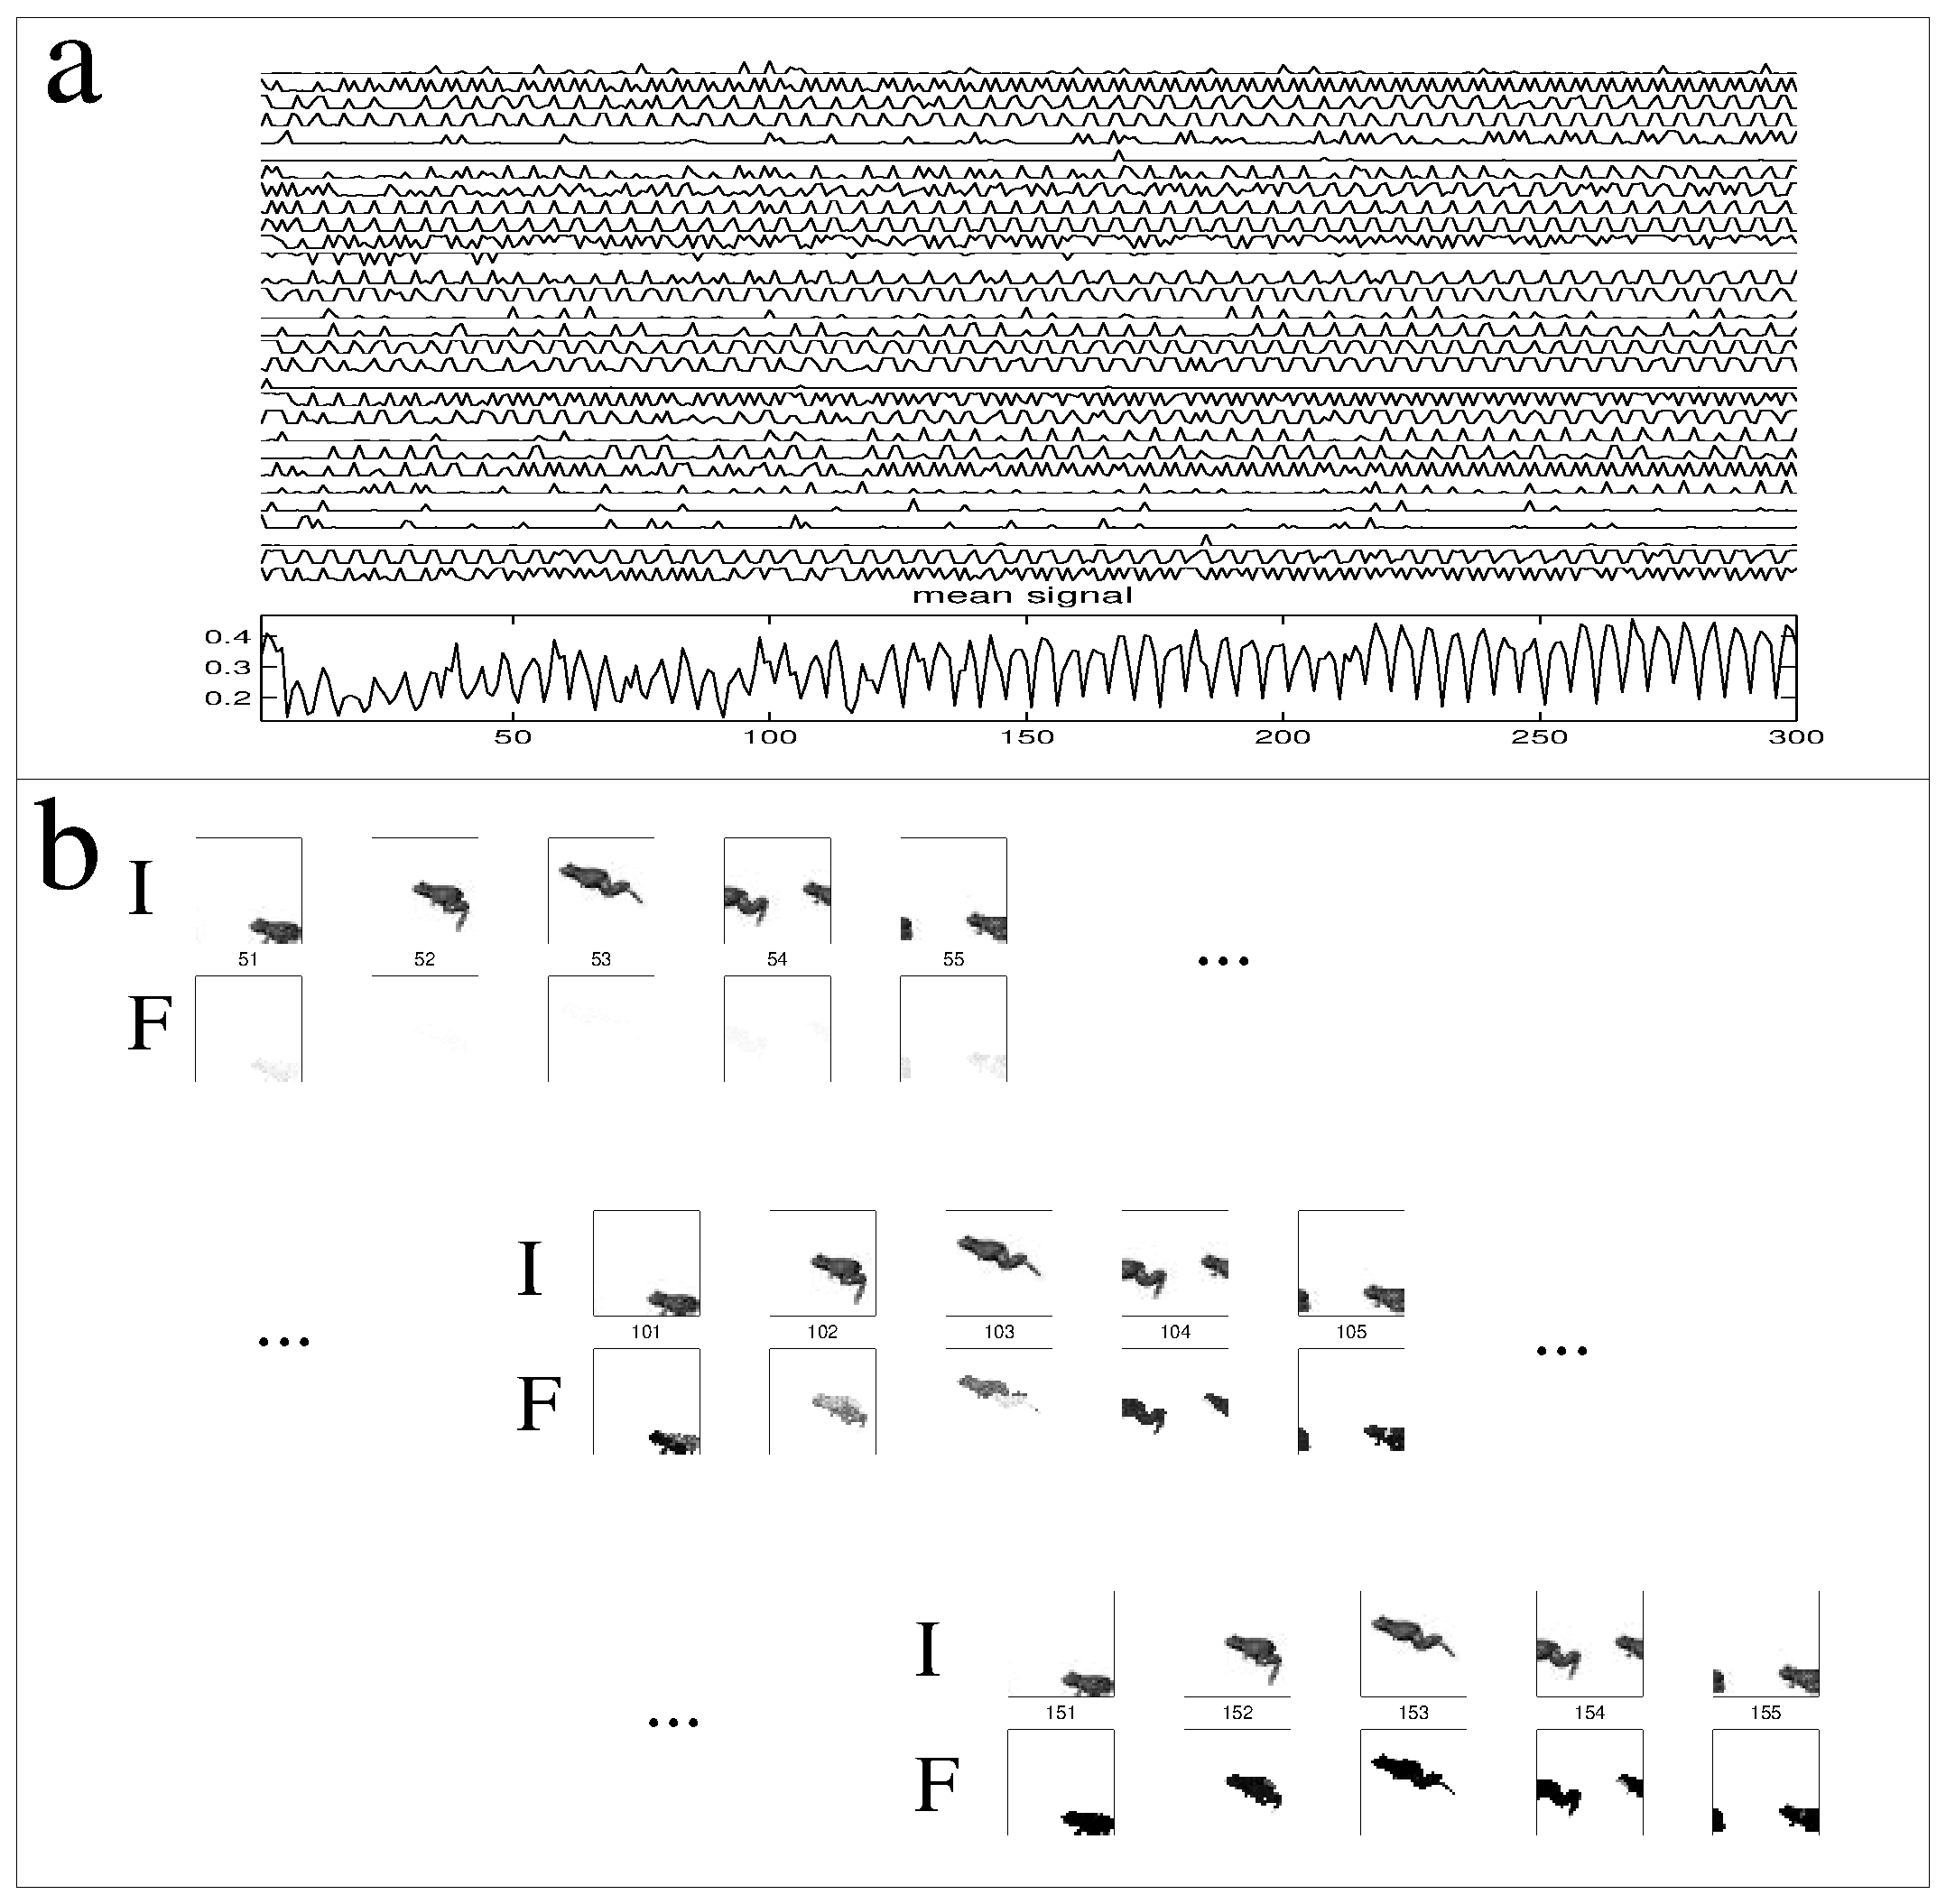
\includegraphics[width=\linewidth]{figs/bc_fig2.eps}
	}
\caption{\footnotesize{Learning dynamics, between $t=1$ and $t=200$. %(with
$N^{(1)}=1600$, $N^{(2)}=200$). 
The system is continuously
stimulated by a periodic spatio-temporal pattern (a frog jump).
%Parameters are in Tab.\ref{tab_param}. 
{\bf --~a~--} Neuronal
activity on the secondary layer. 30 individual signals (out of 200)
have been represented, and their mean activity is represented
below. {\bf --~b~--} Time evolution of the input signal
$\mathbf{I}(t)$ and feedback signal
$\mathbf{F}(t)$, between $t=51$ and $t=155$ (For
readability, most of the time steps have been discarded). At each
time step, the 1600 values of the input layer are represented as $40\times40$
images, where white corresponds to 0 and black to 1 (in-between
values are gray tones) (from Daucé et al, 2002).} } \label{fig:BC02-app}
\end{figure}

{\color{Gray} L'architecture proposée dans \shortcite{Dau02} implémente un principe de traitement
sélectif de la scène sensorielle, en séparant l'espace des sensations entre ce qui est connu (ce qui produit 
un changement qualitatif sous forme de résonance 
perceptive) et ce qui est inconnu (pas de changement qualitatif).
La reconnaissance se traduit par le franchissement d'un seuil (seuil de ``vigilance''),
favorisant le développement d'une activité 
spécifique qui participe à la consolidation et l'entretien de la résonance.}
Le changement par rapport au modèle à une couche réside dans l'utilisation effective des changements qualitatifs 
induits par la plasticité sous la forme du signal de feedback. 
La plasticité permet de \textit{constituer des processus {\color{Orange} attentionnels} spécifiques à certaines configurations
spatio-temporelles apprises}. Ces configurations connues, en activant une résonance, {\color{Orange} révèlent la nature
des connaissance acquises par le réseau.}


Plusieurs papiers de conférences apportent des éclairages complémentaires sur certains aspects du modèle. 
Le papier de la conférence ICANN 2001 \shortcite{Dau01c} présente une version préliminaire du modèle perceptif à deux couches
avec une règle d'apprentissage légèrement plus simple que celle du papier de Biological Cybernetics. 
Le papier de SAB (2000) \shortcite{Dau00b} comporte une partie montrant l'effet de l'apprentissage sur des signaux mixtes composés
d'une partie statique et d'une partie périodique. L'association apprise entre motifs statiques et motifs dynamiques 
se manifeste alors par un niveau de correlation élévé entre la dynamique induite par les motifs mixtes
et la dynamique induite par les motifs statiques seuls (les activités étant par contre qualitativement différentes).

%%\cleardoublepage
%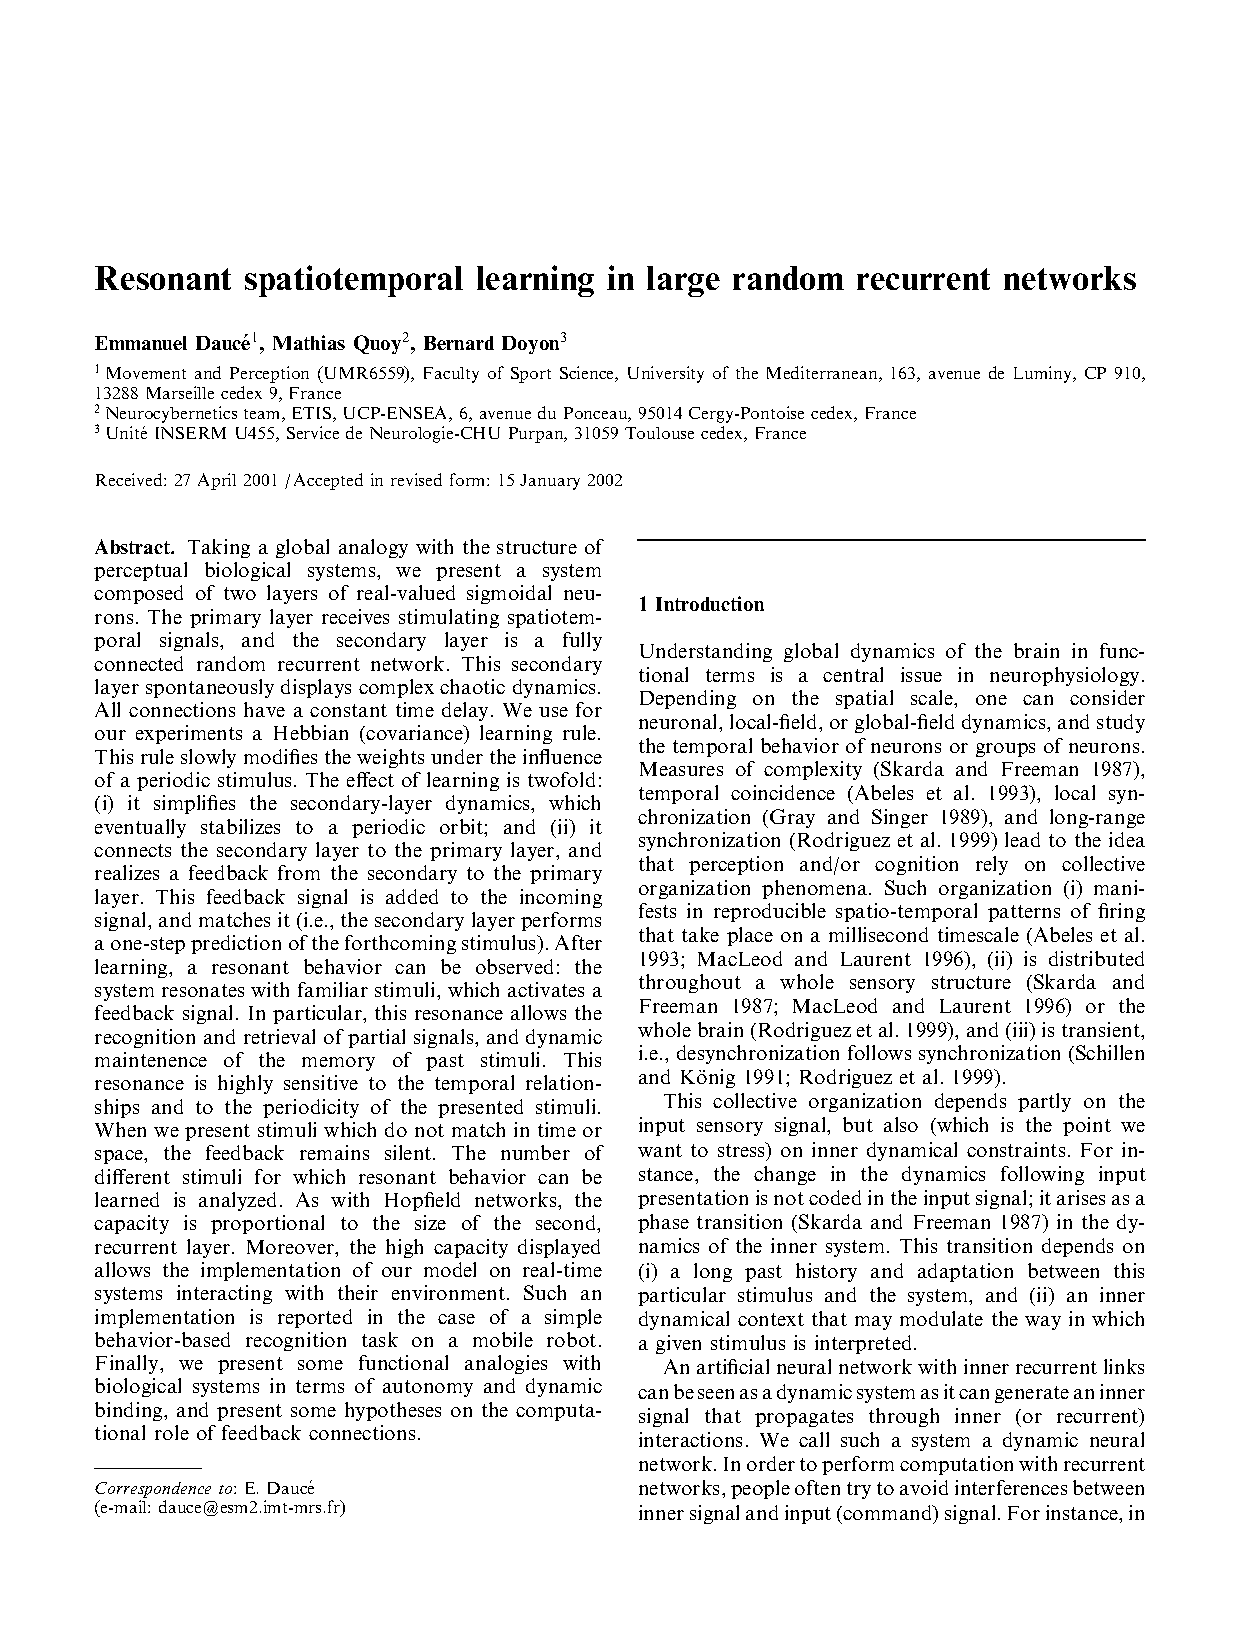
\includepdf[pages=1,offset=70 -30]{pdf/2002-biological-cyb.pdf}
%\includepdf[pages=2,offset=-70 -30]{pdf/2002-biological-cyb.pdf}
%\includepdf[pages=3,offset=70 -30]{pdf/2002-biological-cyb.pdf}
%\includepdf[pages=4,offset=-70 -30]{pdf/2002-biological-cyb.pdf}
%\includepdf[pages=5,offset=70 -30]{pdf/2002-biological-cyb.pdf}
%\includepdf[pages=6,offset=-70 -30]{pdf/2002-biological-cyb.pdf}
%\includepdf[pages=7,offset=70 -30]{pdf/2002-biological-cyb.pdf}
%\includepdf[pages=8,offset=-70 -30]{pdf/2002-biological-cyb.pdf}
%\includepdf[pages=9,offset=70 -30]{pdf/2002-biological-cyb.pdf}
%\includepdf[pages=10,offset=-70 -30]{pdf/2002-biological-cyb.pdf}
%\includepdf[pages=11,offset=70 -30]{pdf/2002-biological-cyb.pdf}
%\includepdf[pages=12,offset=-70 -30]{pdf/2002-biological-cyb.pdf}
%\includepdf[pages=13,offset=70 -30]{pdf/2002-biological-cyb.pdf}
%\includepdf[pages=14,offset=-70 -30]{pdf/2002-biological-cyb.pdf}


%{\color{Violet}
%MECANISME DE DESYNCHRO VITAL POU LE FEEDBACK POSITIF. PASSE PAR DES ``CASSURES''.

%Après apprentissage, la séparation de l'espace d'entrée entre
%signaux connus et signaux inconnus passe par la capacité à provoquer une résonance entre 



%NOTION D'ATTRACTEUR / DISCRETISATION / SIMPLIFICATION / CATEGORISATION

%CARACTERE SUPERVISE / NON SUPERVISE ?

%POINT DE VUE COGNITIF

%POINT DE VUE COMPUTATIONNEL


%L'idée d'un feedback positif comme support de la perception n'est pas nouvelle.
%Il a été postulé de longue date comme support des opérations neuronales. 





%{\bf 1999}

%- reseaux à 2 pop : couche primaire et couche secondaire (perceptive).  Mecanisme de “resonance perceptive” (et “resistance au changement”). Importance des delais. 

%- patrons conditionnants (= contexte)

%- règle de covariance - Règle d’ordre 2 (différence-based / covariance rule) 

%{\bf 2000-2001}

%- Perception par feedback positif. Apprentisage “supervisé par la couche primaire”. La couche primaire est à la fois l’entrée et la sortie.

%(Implicitement : 
%(1) Réseau aléatoire avec delais = réservoir de séquences instables dont certaines s’instancient (“emergence”)
%(2) Predictive coding avant l’heure (de type interpolation)
%(3) Controle moteur “supervisé”

%{\bf Daucé, E., Quoy, M. and Doyon, B. (2002) Resonant spatio-temporal learning in large random recurrent networks, Biol.Cybern. 87(3):185-198}

%- implémentation d’un mécanisme de résonance support de la perception et de la mémoire (en particulier generalisation du principe d’interpolation de Hopfield dans le domaine spatio-temporel). Importance des delais dans le traitement temporel.

%- alternances synchronisation (perçu) / non-sens. Système de perception dual. Figure sur fond (Gestalt). 


%}

%\cleardoublepage
\subsection{Plasticité dans les populations de neurones impulsionnels}
\label{sec:STDP}


En complément de l'analyse des effets de population précédemment mentionnés, j'ai
étudié, dans le cadre de l'ACI ``Temps et Cerveau'',  
les conditions de l'émergence d'oscillations synchronisées \textit{induites} dans des réseaux équilibrés
constitués d'unités binaires (autrement dit neurones impulsionnels sans mémoire).
Les principaux résultats concernant l'application de la plasticité 
sur ces réseaux  sont détaillés dans le papier EPJ-ST de 2007 \shortcite{Dau07} (voir annexe \ref{app:EPJ07}).
Entre autres, 
\begin{itemize}
	\item le papier présente une nouvelle règle de plasticité Hebbienne, 
la règle TD (qui présente des analogies avec la règle des différences temporelles de Sutton et Barto \shortcite{SUTTON98}), qui est 
une règle du premier ordre (voir page \pageref{page:hebb-ordre}) stricte basée sur la conjugaison de l'activité entrante et la \textit{différence d'activité} sortante~:
$$\dot{J}_{ij} - F((s_i^\text{out}(t)-s_i^\text{out}(t-1)) \times s_j^\text{in}, J_{ij})$$
\item 
L'étude présente en premier lieu une région paramétrique dans laquelle on peut observer des transitions entre 
un régime de faible activité et un régime chaotique synchronisé, en fonction du coefficient de variation 
(une moindre variabilité des poids produisant ici un régime plus chaotique).  
\item 
En partant d'un de ces régime à activité faible non-synchronisée, la plasticité 
a pour effet de produire une transition vers un régime à activité synchronisée. 
La passage d'une activité non-synchrone à une activité synchronisée est spécifique aux réseaux équilibrés
(la synchronisation à grande échelle reposant sur les effets de balancier entre population excitatrice et inhibitrice).
\item
Comme dans les autres études, il est possible d'appliquer la plasticité lorsque le réseau
est soumis à un motif statique. Dans ce cas, la plasticité inscrit dans le réseau des comportements
spécifiques (ici de grandes oscillations synchronisées) associées aux motifs appris. 
\end{itemize}



\paragraph{}
Le travail sur des modèles plus réalistes biologiquement a été réalisé, en co-direction avec Gilles Montagne, sur le projet de thèse de
Frédéric Henry, étudiant du master de sciences cognitives à Lyon (voir section \ref{sec:bio}).

Frédéric Henry a travaillé sur un simulateur de réseaux de neurones impulsionnels~:
\begin{itemize}
	\item simulant des délais de transmission variables entre les différents
	neurones
	\item implémentant différentes règles de plasticité synaptique, dont la STDP (Spike-Timing Dependent
	Plasticity).
\end{itemize}



\paragraph{STDP}

La plasticité dépendante des instants de tir (\textit{Spike-timing dependent plasticity} -- STDP)  est  une règle de plasticité dépendant de l'ordre de tir des neurones pré-synaptique et post-synaptique.
%L'utilisation d'une échelle temporelle fine permet d'améliorer le principe Hebbien~: %de transformation de la conjugaison
%d'activité en causalité. 
Cette règle est facilitatrice pour les synapses où l'activité 
pré-synaptique précède causalement l'activité post-synaptique, et, à
l'inverse, suppressive pour les synapses où l'activité post-synaptique précède (de manière anti-causale) l'activité pré-synaptique.
Cette règle tend donc à favoriser les conjugaisons d'activité causalement liées, mais surtout, de manière symétrique, d'empêcher les 
activités non causalement liées. 

La mise en évidence de cette règle sur les synapses naturelles \shortcite{Bi98} a
favorisé le dévelopement de nombreux modèles computationnels~:
\begin{itemize}
	\item  
	Dans des architectures feed-forward,  la STDP  réduit la latence de réponse des neurones 
	aux patrons spatio-temporels appris, permettant d'implémenter un codage par rang \shortcite{song00,guyonneau05}.
	\item 
	Le cas des réseaux récurrents est plus ambigu: 
	\begin{itemize}
		\item dans certaines implémentations, la STDP semble favoriser 
		l'émergence de séquences d'activation stables \shortcite{izhikevich04,izhikevich06}.
		\item 
		D'autres modèles, utilisant une implémentation différente, indiquent une absence de 
		structuration de l'activité, avec des synapses instables sur touts la durée de la simulation \shortcite{morrison07}. 
	\end{itemize}
\end{itemize}


Une formulation possible de la règle est la suivante~:
$$\dot{J}_{ij} = F((s_i^\text{out} \times m_j^\text{in}) - (s_j^\text{in} \times m_i^\text{out} ), J_{ij})$$
où $s_j^\text{in}$ est l'activité pré-synaptique, $s_i^\text{out}$ est l'activité post-synaptique, $m_j^\text{in}$ une trace exponentielle de l'activité pré-synaptique, et $m_i^\text{out}$ une trace exponentielle de l'activité post-synaptique. Cette règle peut formellement être  aux règles de plasticité d'ordre 1 (voir page \ref{page:hebb-ordre}).

En utilisant la technique de transfert d'échelle temporelle (augmentation du pas de discrétisation d'Euler), il est par ailleurs facile
d'établir la correspondance entre la STDP et la règle TD décrite précédemment \shortcite{Dau07},
comme cela avait déjà été noté par \shortcite{Rao01}.
%L'effet de la STDP sur l'activité des réseaux récurrents aléatoires a d'abord été étudié sur un réseau simple
%constitué de connexions gaussiennes centrées. 


{\color{Gray} \paragraph{Remarque} On notera que l'application alternée d'une plasticité Hebbienne et anti-Hebbienne ouvre la voie
à l'implémentation de mécanismes d'apprentissage par renforcement, 
ainsi qu'à la modélisation des mécanismes de plasticité liés à la récompense et 
à la punition dans le cerveau \shortcite{Barto1995,Schultz1997,Gurney2001}. Ces aspects sont analysés 
plus en détail dans le chapitre suivant.}



\paragraph{STDP dans les réseaux récurrents aléatoires} 
L'étude présentée dans \shortcite{Hen08B} 
est motivée par de nombreuses observations sur le rôle des oscillations 
et de la synchronisation dans le fonctionnement du système nerveux.
Les réseaux aléatoires équilibrés offrent, comme on l'a vu (section \ref{sec:balanced}), la possibilité de développer des régimes 
dynamiques plus variés, permettant en particulier la production d'oscillations synchronisées de
grande amplitude dans certaines configurations.
Il est intéressant dans ce cadre d'étudier comment la plasticité interagit avec la dynamique de population 
pour produire des comportements nouveaux, en particulier des oscillations synchronisées.

Les modèles de neurones impulsionnels présentés dans \shortcite{Hen08B,Dau14a} montrent, à une échelle temporelle fine, une capacité
à produire une bouffée d'activité de population (sur une soixantaine de millisecondes), suivie par un retour
à l'état de base. 
Les dynamiques contraintes 
relaxent vers des régime présentant le même degré de chaos que la dynamique spontanée.
Seule la répartition des niveaux d'activité varie.
Les réponses induites par les motifs ne sont pas qualitativement différentes.

Plusieurs indicateurs de complexité ont été mis en place pour mesurer la nature des dynamiques spontanée et induite.
L'analyse du spectre de Fourier ne permet pas d'établir de fréquence caractéristique.
L'autocorrélogramme du signal moyen montre une décroissance exponentielle caractéristique d'un bruit lissé. 
Nous utilisons également un indicateur du nombre de degrés de liberté (basé sur l'ACP \shortcite{wright01}) qui montre
une dimension intrinsèque du signal de l'ordre de 35 pour un réseau de 100 neurones, ce qui indique
une très faible corrélation entre l'activité des différents neurones.
Le réseau développe donc un régime de chaos fort.

Pour séparer les réponses, on applique la STDP sous l'influence
d'un motif particulier. Selon les gammes de paramètres, deux effets peuvent être observés. Dans
certains cas \shortcite{Hen08}, un régime synchronisé est obtenu avec de grandes oscillations 
et une période de l'ordre de 50 à 100 ms (10-15 Hz), lorsque la dynamique est soutenue
par la stimulation (et s'éteint en l'absence de stimulation). Dans ce cas, la dynamique 
finale s'éteint puis renait périodiquement sous
l'effet de la stimulation externe. Dans d'autres cas, le régime est très proche du régime périodique asynchrone
obtenu en dynamique spontanée \shortcite{Hen08B}, avec un comportement ``quasi synchrone'' observable lorsque le
réseau est soumis à des motifs binaires.





\begin{figure}[b!]
	\centerline{
		%\includegraphics[width=4.5cm,height=4cm]{images/dof-nolearn.png}
		\includegraphics[width=.45\linewidth,height=4cm]{figs/dof-learn2.png}
		\includegraphics[width=.45\linewidth]{figs/stdp-homeostatic-spontaneous.png}}
	\centerline{\textbf{a}\hspace{7cm}\textbf{b}}
	\caption{\footnotesize{\textbf{a} \--- Estimated
			number of degrees of freedom during when STDP is
			applied after 5 s of simulation. \textbf{b} \---
			Evolution of the average firing rate when STDP is applied
			for different values of internal coupling (From Henry \& Daucé, 2008).
		}}
		\label{fig:NC08}
	\end{figure} 
	
	
L'application de la STDP conduit la dynamique vers   
un régime plus simple. La dimension intrinsèque décroît continument jusqu'à atteindre une valeur faible (entre 2 et 3),
qui caractérise l'entrée dans un régime périodique  \shortcite{Hen08,Hen08B}. Cette
activité périodique est maintenue de manière asymptotique,
ce qui confirme l'appartenance de la STDP aux règles de plasticité d'ordre 1.
La STDP a également un effet régulateur sur le niveau d'activité moyen. Pour
différents taux d'activité individuels initiaux 
(entre 50 et 400 Hz), la STDP conduit le système vers un régime où l'activité individuelle est de l'ordre de 200 Hz (voir figure \ref{fig:NC08}).
Le caractère régulateur (homéostatique) de la STDP sur le taux de décharge moyen 
est une caractéristique connue déjà notée par \shortcite{KEMPTER99}.

L'activité finale est caractérisée par une périodicité intrinsèque marquée,
de l'ordre de 20 ms (50 Hz). Cette période correspond à environ deux fois le délai moyen \shortcite{Hen08B},
avec une même séquence d'activation qui se répète en boucle.
L'effet de simplification et de stabilisation d'un régime périodique 
dans les réseaux développant activité intrinsèque a été 
moins souvent noté dans la littérature.
Il semble ici être le résultat de la capture de régularités présentes dans la dynamique initiale,
qui se distingue donc d'un pur processus aléatoire.
La différence entre périodicité globale (50 Hz) et activité individuelle (200 Hz) s'explique par le fait
que les neurones tirent en moyenne quatre fois par cycle.

L'activité périodique finale est une activité très robuste. 
Si l'on interrompt l'apprentissage suffisamment tôt, le comportement du réseau permet de séparer l'activité
induite par le (ou les) motif(s) appris de celle induite par les autres motifs \shortcite{Hen08}. 
En optimisant la durée d'apprentissage, une étude (non publiée) montre
une capacité d'encodage similaire à celle des réseaux continus: le nombre maximal de motifs 
pouvant induire une réponse spécifique est de l'ordre de 5\% du nombre de neurones dans le réseau.

{\color{Violet}
	L'étude des effets de la STDP sur la dynamique intrinsèque des réseaux
	récurrents aléatoires indique de nombreux points communs entre les réseaux de neurones à
	sortie fréquentielle et les réseaux de neurones impulsionnels. Des comportements
	qualitativement similaires se retrouvent entre les deux familles de modèles, traduisant 
	une plasticité essentiellement fondée sur les fréquences de décharges.
}
{\color{Gray}
	
	Le résultat de ce schéma computationnel est un fonctionnement par ``\mbox{sauts}'' d'un attracteur à un autre, 
	et une alternance entre destabilisation et stabilité.
	Bien que possiblement implémenté par des équations aux dérivées partielles, la logique
	de ce schéma est donc essentiellement celle d'un fonctionnement discret, voire séquentiel.
}

D'un point de vue computationnel, il n'y a qualitativement pas de différence entre le nouveau modèle et
l'ancien \shortcite{Dau98A}. Le comportement induit par la STDP ne semble donc pas reposer sur l'ordre ou 
l'instant de tir des potentiels d'action, mais plutôt sur leur fréquence de décharge.

\paragraph{STDP dans les réseaux équilibrés}
L'utilisation d'un patron de connectivité plus réaliste a été proposé dans une étude datée de 2009 \shortcite{Henry09},
avec séparation fonctionnelle des neurones excitateurs et inhibiteurs, et utilisation de neurones à 
conductance \shortcite{Kepler1992}. 
Cette étude %sur un réseau équilibré
%permet de mettre 
met en évidence un comportement très analogue à celui observé sur le modèle binaire \shortcite{Dau07},
confirmant la parenté fonctionnelle entre la règle TD et la STDP
(voir \shortcite{Rao01}). 
La STDP est appliquée uniquement sur les connexions 
entre neurones excitateurs. Une convergence vers un régime d'oscillations synchronisées avec une période globales de 
l'ordre de 25 Hz (et une fréquence moyenne individuelle de l'ordre de 200 Hz) est mis en 
évidence. Il s'agit d'une synchronisation observable au niveau de la population, les activités individuelles
restant relativement irrégulières et hétérogènes. Une analyse de la plasticité en fonction des délais met en évidence la potentiation des 
délais longs ($>$ 8 ms) et une dépression des délais intermédiaires (4-8 ms) qui favorise l'entretien du comportement synchronisé (non publié).

%%\cleardoublepage
%\includepdf[pages=1,offset=70 -30]{pdf/2008-NEUROCOMP-ann.pdf}
%\includepdf[pages=2,offset=-70 -30]{pdf/2008-NEUROCOMP-ann.pdf}
%\includepdf[pages=3,offset=70 -30]{pdf/2008-NEUROCOMP-ann.pdf}
%\includepdf[pages=4,offset=-70 -30]{pdf/2008-NEUROCOMP-ann.pdf}
%\includepdf[pages=5,offset=70 -30]{pdf/2008-NEUROCOMP-ann.pdf}


%\cleardoublepage
\paragraph{STDP et action de population}

Une dernière étude, publiée récemment dans les proceedings d'ESANN \shortcite{Dau14a}, étudie l'effet de la STDP 
dans un réseau équilibré sous influence d'un signal spatio-temporel. Deux cas sont considérés : signal périodique
(se répétant toutes les 30 ms) ou signal non-périodique. L'activité spontanée sous influence de ces deux types de signaux
est qualitativement la même initialement. La plasticité est appliquée 
dans les deux situations.
Lorsque le stimulus est apériodique, aucun changement qualitatif n'est observé.
Lorsque le stimulus est périodique, l'activité devient plus régulière, avec 
de grandes oscillations (période 16 Hz) observables au niveau de la population (voir figure \ref{fig:ESANN14}).
Le comportement est assez proche du comportement de grandes oscillations lentes
obtenu sous influence statique. On observe 
néanmoins une synchronisation des oscillations du réseau avec la période 
du stimulus, autrement dit il y a un accrochage de phase de sorte que la période interne (60 ms)
est exactement le double de la période du signal (30 ms). Ce comportement d'accrochage est assez comparable
à celui observé sur les réseaux plus simples. Le réseau devient ``réactif'' aux motifs périodiques appris,
développant une ``action de population'' qui est un analogue global des potentiels
d'action neuronaux.

{\color{Violet}
Une sensibilité acquise à des patrons spatio-temporels spécifiques, telles qu'observée dans les modèles fréquentiels (voir paragraphes précédents), 
peut donc être obtenue à l'échelle de quelques millisecondes, mettant en jeu un faible nombre de spikes par neurone.
Le même mécanisme peut donc être identifiés à différentes échelles, les opérations
à échelle temporelle courte étant elles-même possiblement ``portées'' (ou embarquées) dans des opérations à échelle temporelle plus larges.
}


\begin{figure}[t!]

\centering{
\begin{tabular}{cc}
\includegraphics[width=7.8cm,height=10.4cm]{figs/simu4bis.eps}&
\includegraphics[width=7.8cm,height=10.4cm]{figs/simu7bis.eps} \\
\textbf{-A-}&\textbf{-B-}
\end{tabular}
}
\caption{\footnotesize{Excitatory population activity during STDP learning. -A- Non-periodic input -B- Periodic input (from Daucé, 2014).}}
\label{fig:ESANN14}
\end{figure}


%
%%\cleardoublepage
%\includepdf[pages=1-2,landscape=true,nup=1x2,scale=1.1,offset= 80 -30]{pdf/2014-esann-A-ann.pdf}
%\includepdf[pages=3-4,landscape=true,nup=1x2,scale=1.1,offset= -80 -30]{pdf/2014-esann-A-ann.pdf}
%\includepdf[pages=5-6,landscape=true,nup=1x2,scale=1.1,offset= 80 -30]{pdf/2014-esann-A-ann.pdf}

%{\color{Violet}
%Fred Henry : Master en 2005.

%bourse these : 
%juin 2005 Ste Marguerite (initiation de neurocomp)

%These Fred : pb : le lien avec le mouvement?

%* 2005-2006 * 

%oct. 2005 NOLTA - 

%jan 2006 institut H Poincaré - 

%juillet 2006 CNS à Edinbourg (modèle Gaussien du Master)

%* 2006-2007 *

%Dyva en sept 2006 présenté par Fred - idées orientées neural field + colliculus + LIF simple

%oct. 2006 premiere conf. Neurocomp - 
%idées RL + couche récurrente intermédiaire. 
%Policy Gradient (Bartlett) = local changes = Hebb/anti-Hebb
%Idée d'interversion bruit/signal dans les modèles à 2 couches (Gaussiennes centrées?).
%Illustration avec simu Khepera.

%juin 2007 - NIPS (refusé). 
%modèle LIF/SRM à courant (avec free mb. potential h). 
%- Connexions gaussiennes centrées . DELAI FIXE (10 ms)
%STDP --> activité périodique non synchronisée

%papier EPJ-ST : modèle RL Hebb/anti-Hebb avec terme (1-H) (comme SAB) sur liens excitateurs - separation exc/inh.

%* 2007-2008 *  

%Dyva en sept 2007 (signé Daucé) - poursuite approche RL-PG appliquée aux saccades.
%(Fred ne participe pas à ce projet)

%ESANN avril 2008 : idem NIPS sauf DELAI VARIABLE (Poisson moy. 10 ms). STDP produit oscillations lentes. entrée = POTENTIEL.

%Tentative publi dans neurocomputing - echec. (calcul plus fin de la ``loading capacity'' - !! sur ordi Centrale only)

%* ATER Lille 2008-2009 *

%oct. 2008 - 2eme Neurocomp. Distinction input courant/input potentiel. differents regimes sont obtenus selon le type
%d'input / les parametres internes.

%juillet 2009 : CNS - séparation excitateurs/inhib. Plasticité sur exc. seulement. delais variables. effet 
%stdp sur delais.

%septembre 2009 : suite projet RL. 

%ACI 'temps et cerveau' va de 2002 à 2007 (5 ans???)

%MAPS commence en septembre 2007 (le dossier a été monté en janvier-février 2007)


%{\bf 2008}
%- modèles à 2 couches (strictly excitatory/inhibitory). 

%{\bf 2009}

%- “Free membr. potential” (synaptic input) / modeles ECM à “horizon fini” 

%Mean field

%Mon apport :
%- Multi-pop
%- Délais
%- frontiere
%- contrib. Reseaux equilibrés --> comportementdes réseaux équilibrés à la frontière

%On-off states?



%{\bf 2008}

%- Balanced networks et STDP.

%{\bf 2014}

%- population response (population “spike”) avec STDP. Importance des termes de reequilibrage des poids et de la SFA.  Idée de multi-échelle et de detecteur d’information mutuelle à travers l’activité. Idée de STDP comme sequence enhancement.

%UP/DOWN

%Brunel

%Frequences, rythmes, periodicités


%}

%%%%%%%%%%%%%%%%%%%%%%%%%%%%%%%%%%%%%%%%%%%%%%%%%%%%%%%%%%%%%%%%%%%%%%%%%%%%%%%%%%%%%%%%%%%%%%%%%%%%%%%%%%%%%%%%%%%
%%%%%%%%%%%%%%%%%%%%%%%%%%%%%%%%%%%%%%%%%     2.4      %%%%%%%%%%%%%%%%%%%%%%%%%%%%%%%%%%%%%%%%%%%%%%%%%%%%%%%%%%%%
%%%%%%%%%%%%%%%%%%%%%%%%%%%%%%%%%%%%%%%%%%%%%%%%%%%%%%%%%%%%%%%%%%%%%%%%%%%%%%%%%%%%%%%%%%%%%%%%%%%%%%%%%%%%%%%%%%%
%\cleardoublepage
\subsection{Discrimination de séquences spatio-temporelles}\label{sec:discri}

Les protocoles d'apprentissage présentés jusqu'à présent avaient pour but de 
former une réponse induite. La forme de la réponse n'était pas 
fixée à priori et dépendait des caractéristiques du substrat.
Il n'y avait pas de ``read-out'', il s'agissait juste de produire une dynamique de relaxation qui se 
conforme à (prenne forme avec) la contrainte imposée, en rendant le réseau plus réactif à certains 
motifs présentés.

\begin{figure}[t!]
\centering
\includegraphics[width=\linewidth]{figs/archi.png}
\caption{ \footnotesize{{\bf Experimental setup}. $N$ temporal patterns are to be presented to the network 
in order to be classified in $K$ categories. The network is composed 
of three populations. The input layer is composed of 4 neurons (labeled A, B, C and D). 
The input connections follow a random Gaussian law of mean zero and standard 
deviation 0.04. The hidden layer contains 100 fully connected neurons. The 
recurrent connections follow a random Gaussian law of mean 0 and standard deviation 
of 0.02. The output layer is composed of $K$ neurons, with lateral inhibition (not represented).
The output connections follow a random gaussian law of mean 0.09 and standard 
deviation 0.01 (from Henry et al., 2007).}}
\label{fig:3layer}
\end{figure}



Dans une étude antérieure datant de 2006, nous avons également considéré une architecture 
à entrées-sorties complète~:
\begin{itemize}
	\item
Le réseau possède une couche d'entrée qui 
transmet passivement le signal, une couche récurrente aléatoire, et une couche de sortie
constituée dans ce cas de quelques neurones dont la sortie est lue.
\item
La forme de la réponse induite est imposée par l'expérimentateur,
de manière supervisée ou semi-supervisée.
\end{itemize}

La tâche consiste à discriminer quatre motifs spatio-temporels.
Ces motifs possèdent des éléments en communs, de telles sorte qu'il est impossible de séparer les signaux
sur la base de l'entrée instantanée.
Chaque neurone de sortie représente une catégorie.
La réponse est fixée par le neurone qui émet le premier potentiel d'action suite
à la présentation du motif (voir figure \ref{fig:3layer}).

Le protocole d'apprentissage consiste à présenter les séquences périodiquement, 
lire les réponses produites, informer le réseau du caractère correct ou incorrect de sa
réponse et appliquer une règle de plasticité visant à augmenter le taux de réponses correctes, selon
un principe qui se rapproche de l'apprentissage par renforcement.

L'apprentissage utilise sur les effets symétriques des règles Hebbienne et anti-Hebbienne 
sur la dynamique des réseaux récurrents aléatoires, montrés dans \shortcite{dauce05}.
Par exemple, l'anti-STDP (règle miroir de la STDP) a pour effet d'augmenter la complexité
de la dynamique intrinsèque, soit un effet contraire à la STDP. L'application successive
de la STDP puis de l'anti-STDP sur un réseau récurrent aléatoire 
a pour effet de réduire la complexité puis de l'augmenter à nouveau.

L'étude est également une implémentation originale du codage par rang, utilisant un principe 
concurrent d'avance vs. retard de la réponse.
Si la réponse est correcte, la STDP est appliquée sur la couche de sortie et sur la couche récurrente,
ce qui tend à anticiper l'instant de réponse du neurone ayant tiré.
Si la réponse est incorrecte, c'est l'anti-STDP qui est appliquée, 
tendant à retarder la réponse.
Le papier \shortcite{henry07} utilise des signaux temporels très lents, où
la séquence est composée de 4 motifs durant chacun 100 ms, de sorte qu'une séquence
complète dure 400 ms. Dans ce cas, le temps nécessaire pour atteindre des taux
de réussite raisonnables s'exprime en heures (environ 100000 essais).
Les résultats présentés dans \shortcite{Dau06} utilisent des séquences plus courtes (40 ms).
Dans ce cas, environ 500 essais suffisent pour obtenir une discrimination parfaite.

La différence de taux d'apprentissage et de taux de réussite s'explique principalement par 
la différence d'échelle temporelle des séquences à apprendre. La mémoire d'une unité neuronale est de l'ordre de
sa constante de membrane, soit 10 à 20 ms.
Néanmoins, à la
lumière des résultats du chapitre précédent, la plasticité semble 
capable d'induire suffisamment de régularité dans la dynamique intrinsèque
pour conserver une mémoire plus importante 
au sein de la population. La difficulté à discriminer les séquences de 400 ms semble
néanmoins fixer la limite supérieure de cette capacité (100 ms étant en pratique suffisant 
pour discriminer deux séquences).

%%\cleardoublepage
%\includepdf[pages=1,offset=70 -30]{pdf/2007-neurocomputing.pdf}
%\includepdf[pages=2,offset=-70 -30]{pdf/2007-neurocomputing.pdf}
%\includepdf[pages=3,offset=70 -30]{pdf/2007-neurocomputing.pdf}
%\includepdf[pages=4,offset=-70 -30]{pdf/2007-neurocomputing.pdf}
%\includepdf[pages=5,offset=70 -30]{pdf/2007-neurocomputing.pdf}
%\includepdf[pages=6,offset=-70 -30]{pdf/2007-neurocomputing.pdf}
%\includepdf[pages=7,offset=70 -30]{pdf/2007-neurocomputing.pdf}
%\includepdf[pages=8,offset=-70 -30]{pdf/2007-neurocomputing.pdf}

%{\color{Violet}
%{\bf 2005}



\chapter{Architectures de contrôle}

\textit{Ce chapitre aborde la question plus globale de la formation des comportements moteurs. 
	Nous commençons par rappeler certains principes et problèmes d'ordre général, comme la différence d'extensivité et d'expressivité du contrôleur et de son environnement.
	Nous présentons ensuite un certain nombre de résultats ayant en commun le principe du contrôle en ``boucle fermée''.
	Nous abordons ainsi successivement la question de la stabilisation et de la déstabilisation des patrons d'interaction
	vus comme des transitions entre activité autonome et activité commandée, et la question de l'activité autonome (chaos, bruits ``structurés'') pour l'implémentation
	des mécanismes d'exploration dans le cadre de l'apprentissage par renforcement, sur divers substrats neuromimétiques. 
	De manière plus appliquée, nous détaillons les principes d'une architecture de contrôle destinée à supplémenter des déficiences
	motrices à partir de l'analyse de l'EEG de surface (interfaces cerveau-machines non-invasives).}

{\color{Cyan} 

\begin{itemize}	
\item Langage de l'action. 

\item Espace de la tâche. Passage d'échelle et variable d'ordre.

\item Scène sensorielle et scène motrice

\item Facteurs causaux.

\item La tâche. L'espace de la tâche (Marr) = niveau computationnel.

\end{itemize}
}

\section{Notions générales}

{\color{Cyan} Cette section présente un formalisme et des définitions visant à ...}

\subsection{Contrôleur et environnement}

L'approche dite ``située'' en robotique
mobile et en intelligence artificielle \shortcite{Bro91,Varela91} prône la prise 
en compte de la contrainte du corps
comme élément structurant du développement de {\color{Orange} capacités cognitives} plus élaborées.
{\color{Orange} Cette contrainte, qui s'exprime par les {\bf dépendances sensori-motrices}, et 
la prise en compte des {\bf disparités d'échelle}, augmente néanmoins considérablement 
la complexité des tâches
d'apprentissage et de leur implémentation par plasticité synaptique. }

Le cadre que nous considérons ici est celui de la commande motrice. Nous considérons un programme doté d'effecteurs moteurs capables de déplacer et faire pivoter des masses articulées dans l'espace physique.  L'espace physique est décrit, d'une part, par ces effecteurs directement contrôlables, ainsi que d'autres éléments physiques non directement contrôlables. 
\begin{itemize}
	\item Le programme est le \textit{contrôleur}.
	\item L'espace physique est l'\textit{environnement}.
\end{itemize}  

L'interaction d'un contrôleur avec son environnement passe par des transducteurs, qui sont les canaux de 
communication entre les deux milieux~:
appareils sensoriels et proprioceptifs chez les animaux, et contractions musculaires permettant de déplacer des masses
articulées; senseurs et actuateurs pour les dispositifs de contrôle artificiels : capteurs qui traduisent des signaux physiques
en signaux électriques, moteurs, joints et pistons pour les déplacements de masses.


Le cadre que nous avons regardé jusqu'à présent est l'apprentissage en ``boucle ouverte'',
dans lequel les actions physiques sur le milieu sont découplées des sensations. 
{\color{Gray} C'est le cadre classique du conditionnement Pavlovien où les stimuli déclenchent
des réponses comportementales automatiques ou induites par l'apprentissage.}
La prise en compte plus réaliste
des deux domaines matériels que sont le circuit logiciel et le milieu physique
environnant conduit à déplacer 
le cadre conceptuel de l'apprentissage vers l'apprentissage en ``boucle fermée''.
Il se définit formellement par la présence de corrélations entre les actions ou 
les réponses produites et les manifestations sensorielles suivantes.



\subsubsection{Tâches et problèmes de contrôle}

Le contrôle en boucle fermée \cite{Wiener1965}
consiste à programmer le contrôleur de telle sorte que les actions produites dans le milieu se conforment à un certain nombre de critères (ou contraintes) définis \textit{a priori}.	
Ces critères peuvent être :
\begin{itemize}
	\item le caractère non délétère des actions produites (endommagement du dispositif moteur ou de l'environnement)
	\item la minimisation de certaine dépenses (consommation énergétique, effort, usure, chauffage des composants, ...)
	\item la rapidité de la réponse
	\item la résilience, la capacité à résister aux perturbations (homéostasie)
	\item la stabilité et la reproductibilité des réponses, la robustesse.
	\item etc. 
\end{itemize}

Ces problèmes ont été analysés de longue date dans le cadre de la théorie de l'automatique (contrôle linéaire) et de la commande optimale, en particulier sous l'angle de la stabilité de la réponse à la commande et de l'homéostasie {\color{Orange}[REFS]}.

La théorie du contrôle classique décrit un problème de contrôle comme un problème d'optimisation basé sur~:
\begin{itemize}
	\item une consigne, correspondant à un état nominal $\boldsymbol{x}^*$ dans lequel on souhaite voir le milieu physique,
	\item un contrôleur doté de capteurs et d'actuateurs,
	\item et le milieu physique situé dans l'état $\boldsymbol{x}_\text{out}$.
\end{itemize}

Le problème d'optimisation consiste à programmer une fonction de réponse $\phi_\text{in}$ qui, étant donnée une consigne $\boldsymbol{x}^* \in \mathcal{C}$, conduit le milieu physique dans l'état désiré. 


{\bf Exemple~}: Dans le cas d'un bras mécanique, $\boldsymbol{x}_\text{out}$ peut décrire les coordonnées spatiales d'un effecteur et $\boldsymbol{x}^*$ la position finale désirée.

{	\color{Gray}Dans le cadre de problèmes de robotique, on distingue généralement~: 
	\begin{itemize}
		\item l'espace de la tâche (par exemple atteindre une certaine position de l'espace  avec l'extrémité du bras)
		\item et l'espace des articulations, décrivant le détail des positions des éléments mécaniques composant le robot.
	\end{itemize}	
	Pour une position finale unique, il existe en général plusieurs configurations des articulations. 
}

\paragraph{Remarque~:} Il est possible d'établir une analogie entre consigne et programme. Une consigne s'apparente plus précisément à un \textit{programme moteur} qui conditionne la manière dont le contrôleur traite ses entrées sensorielles~: pour deux consignes différentes, les mêmes entrées sensorielles ne produisent pas la même réponse.  

\subsubsection{Rétroaction négative vs. contrôle balistique}

 Le principe de contrôle par rétroaction négative (\textit{negative feedback control})  correspond à une commande directement proportionnelle à l'erreur motrice, autrement dit $\boldsymbol{u}(t) \propto \boldsymbol{x}^* - \boldsymbol{x}_\text{out}(t)$. En tenant compte de l'inertie et des temps de réponse, il permet d'obtenir un contrôleur homéostatique stable  (résistant aux perturbations). 
 
 La différence $\boldsymbol{x}^* - \boldsymbol{x}_\text{out}(t)$ est appelée l'\textit{erreur motrice}.
  
 On oppose au contrôle par feedback négatif le contrôle dit \textit{balistique} dans lequel l'erreur motrice n'est pas mesurée. Le contrôle repose sur la consigne $\boldsymbol{x}^*$ seule. On parle aussi de contrôle en position. 
 
 Plusieurs méthodes permettent d'implémenter ce type de contrôle:
 \begin{itemize}
 	\item Dans le cadre du contrôle linéaire, la commande balistique repose sur l'inversion de la fonction de transfert de l'environnement. Si $\boldsymbol{x}^*$ est la position finale désirée, on a $\boldsymbol{u} =  \phi_\text{out}^{-1}(\boldsymbol{x}^*)$. On parle de commande par modèle inverse.
	\item Le cas des modèles non-linéaires peut être traité via  la combinaison de ``primitives motrices'' dans l'espace de la tâche \shortcite{Mussa2004}.
%\subsubsection{Erreur motrice et erreur de prédiction}

\end{itemize}

Le contrôle balistique présente plusieurs propriétés intéressantes~:
\begin{itemize}
	\item la commande $\boldsymbol{u}$ reste constante pendant toute la durée d'exécution.
    \item la commande est insensible aux conditions initiales. Quelle que soit la position initiale du contrôleur, la commande conduit ``mécaniquement'' le système contrôlé vers son point fixe $\boldsymbol{x}^*$. %
    \item le contrôleur est insensible à ses entrées sensorielles. Autrement dit la conséquence sensorielle de la commande n'est pas utile pour le contrôle lui-même. Le signal mesuré sur les capteurs peut néanmoins conduite le contrôleur à \textit{réviser la consigne} si le signal d'entrée  n'est pas conforme au signal attendu.
\end{itemize}

Une version ``dynamique'' du contrôle balistique a été proposée par \shortcite{Schoner97}, dans laquelle~:
\begin{itemize}
	\item la commande motrice est implémentée sous la forme d'un champ de potentiel dans l'espace de la tâche  (combinaison de champs de force);
	\item la consigne évolue continuellement en fonction des entrées sensorielles.
\end{itemize} 
 


%La fonction $\phi_\text{in}$ est dans ce cadre une fonction paramétrique, décrite par l'ensemble de paramètres $\Theta$.
%Le problème d'apprentissage se présente alors comme un problème d'optimisation, où la mise à jour des paramètres repose sur l'optimisation d'un certain critère $\mathcal{H}$ lié à la qualité du contrôle opéré par le contrôleur.

%\begin{align}
%\min_{\Theta}  \mathcal{H}(\theta)
%\end{align}



%Dans le cadre probabiliste défini plus haut, On note   la distribution jointe portant sur l'état latent de $\boldsymbol{x}$ estimé via un processus de mesure paramétré par   distribution estimation de  $\boldsymbol{x}$  on pourra définir le modèle interne $P$ et la mesure $Q$ comme des lois paramétrées par $\Theta$, i.e.   



{\color{Gray}L'apprentissage en boucle fermée consiste à produire des ajustements 
qui améliorent les interactions du logiciel avec le milieu physique, en tenant compte des boucles de rétroaction entre les commandes motrices et les signaux sensoriels.}










{\color{Gray}  En considérant principalement des consignes statiques, le problème peut s'exprimer comme~:
\begin{align}
\min_{\Theta}  \int_{\mathcal{C}} \lim_{t\rightarrow\infty} ||\boldsymbol{x}^* - \boldsymbol{x}_\text{out}(t)||^2 d\boldsymbol{x}^*
\end{align}
où l'ensemble $\mathcal{C}$,  continu ou discret, est l'ensemble des consignes (ou tâches) possibles.

Une manière plus ``dynamique'' de présenter le problème d'optimisation est :
\begin{align}
\min_{\Theta}   \int_{\mathbb{R}^+} ||\boldsymbol{x}^*(t) - \boldsymbol{x}_\text{out}(t)||^2 dt
\end{align}
où 	$\boldsymbol{x}^*(t)$ est une consigne variant au cours du temps.

	Un autre problème consiste à choisir une commande motrice telle que l'erreur de prédiction (et non plus l'erreur motrice) soit minimisée {\color{Orange}[DEAN,FRISTON]}.
	
	Le problème devient~:
	\begin{align}
	\min_{\Theta}   \int_{t \in \mathcal{T}} ||h_\text{in}( \boldsymbol{x}^*(t)) - \boldsymbol{I}(t)||^2 dt
	\end{align}	
	}

\subsubsection{Apprentissage sans consigne}

Avec modèle : la programmation dynamique.


\subsubsection{Apprentissage du modèle}

EM

Friston(?). Rôle de la complexité.

{\color{Cyan}   Dynamical Causal modelling.
	``{\emph Modern reformulations suggest
		that both inference on states (that is, perception) and
		inference on parameters (that is, learning) minimize
		free energy (that is, minimize prediction error) and
		serve to bound surprising exchanges with the world.}'' (Friston, 2010)
	
	
}

\subsubsection{Apprentissage sans modèle}

\paragraph{Exploration motrice}
%L'exploration motrice. Babbling.

%{\color{Purple} 

Considérons un dispositif logiciel contrôlant un appareil 
ayant des interactions répétées avec son milieu.
Dans des environnements complexes où il est difficile de tout prévoir, la machine doit 
adapter son comportement face aux situations particulières qui se présentent.
{\color{Orange} Ce cahier des charges rejoint l'idée de méta-programme : il s'agit de produire des ajustements 
qui améliorent les interactions du logiciel avec le milieu physique. }


Un tel problème se formule de différentes manières.
 Une première approche consiste à faire en sorte que le logiciel enrichisse le modèle du monde, 
 c'est à dire ``acquière des connaissances'' pour mieux prévoir les effets de ses actions sur 
 son environnement. Cette phase d'acquisition passe par le fait de ``tester'' le produit
 de ses actions par essai/erreur. Le simple fait de produire une commande arbitraire
 (aléatoire) permet de tester la conséquence sensorielle de cette commande, qui peut
 être confrontée au modèle, utile en particulier pour l'apprentissage
 des contingences sensori-motrices \shortcite{Andry2001}.
 
 
 %}

{\color{Cyan} Tout l'AR


	Action based. RL classique. Analogie etat caché / valeur (sortie du modele representationnel. L’etat interne ne represente pas l’etat du monde exterieur mais simplement l’avantage qu’on peut en attendre.

Model free -  Policy gradient. Apprentissage direct du repertoire d’actions	
	
	
	-Friston: le reward est un prior sur la solution cherchée.
	
	 Rq : le couple (actionneurs + environnement = systeme controllé = domaine extensif - masses en deplacements) est en general connu , c’est à dire qu’on a une connaissance complete. Le couple acteur + critique est l’agent - domaine intensif). 

}
	 
\paragraph{Dilemme exploration exploitation.}

Le dilemme exploration/exploitation, exprimé sous sa forme la plus simple 
comme un problème d'échantillonnage aléatoire de l'espace des choix (problème dit du ``bandit manchot'').
Chaque tirage apporte une information qu'il convient d'exploiter au mieux, en établissant un compromis
entre recherche d'information (réduction d'incertitude) et exploitation effective de l'information 
(pour maximiser le gain).
Cette forme d'apprentissage séquentiel établit des modèles qui visent à réduire 
la différence entre les gains obtenus par l'algorithme et les gains
attendus en toute connaissance de cause.
L'apprentissage séquentiel statistique est le socle d'une famille de méthodes d'apprentissage 
fondée sur l'échantillonnage de l'environnement, comme le Q-learning ou le TD-learning dans le
cadre de l'apprentissage par renforcement classiques. Cette approche a renouvelé le domaine, en proposant 
par exemple des politiques non-stochastiques (algorithme UCB), ou en étendant le modèle au cas ``adversarial'' 
(théorie des jeux) \shortcite{Auer2002}. 

	 
\paragraph{Temporal credit assignment}

Cette importance de la commande aléatoire dans l'acquisition de connaissance a été formalisé
dans le cadre de \textit{l'apprentissage par renforcement} \shortcite{SUTTON98}
Cette approche repose sur la notion de signal de renforcement, qui est un ``méta signal'' 
dont le rôle est de transformer le manière dont le logiciel traite le signal,
selon des modalités variées comme la consommation énergétique, l'exposition aux signaux nociceptifs ou bénéfiques, 
ou encore la réduction d'incertitude.
Si le milieu contient des éléments nocifs ou aversifs par exemple, l'amélioration 
peut passer par une augmentation de la sensibilité logicielle à une classe de signaux 
associés à (ou précurseurs de) la sensation aversive, et à une facilitation des comportements permettant de
mieux éviter les situations où le signal aversif est présent. 
La plupart des modèles de renforcement reposent sur des tables de correspondance (``Look-up table''), adaptées
aux environnements et aux choix d'action discrets, mais souffrent de problèmes
d'explosion combinatoire dans des environnements continus et/ou complexes.

Une séance d’apprentissage consiste à effectuer une série de ``choix'' qui orientent
le cours futur de la séance. 
La tâche n'est plus définie par rapport à la justesse des réponses instantanées, mais par rapport
à la justesse de ce parcours dans l'espace des trajectoires possibles.

Les signaux de renforcement (méta-signaux) servent à ``sculpter'' le programme
au cours des interactions entre le logiciel et son environnement.
Le programme qui résulte de ces interactions varie 
selon l'expressivité du réseau sous-jacent (la structure du circuit logique),
le caractère déterministe ou stochastique des politiques d'exploration
et enfin le caractère convexe ou non de la tâche. 
Le choix entre les réponses peut être départagé selon l'espérance de récompense 
associée à chacune d'elles, mais aussi selon le degré d'incertitude associé, 
certaines réponses mal connues (ou certaines sources et/ou chemins mal modélisés) pouvant potentiellement apporter des 
récompenses supérieures. C'est le fameux dilemne ``exploration/exploitation''.





\subsubsection{Plasticité de Hebb}
Nous étudions, comme dans les chapitres précédents, l'apprentissage sous l'angle de la plasticité, en particulier la plasticité synaptique
de Hebb. %La plasticité consiste, comme nous l'avons vu, à appliquer des petits changements aux paramètres de la fonction de réponse du contrôleur.  
Dans le cadre des modèles de réseaux de neurones, il s'agit essentiellement de modifier les poids synaptiques $J_{ij}$ entre les nœuds du graphe.

En reprenant les notations proposées dans les chapitres précédents (e.g. les équations (\ref{eq:SD-plast-x}) et (\ref{eq:SD-plast-J})), la matrice $\boldsymbol{J}$ décrit les poids du réseau de neurones et l'évolution de cette matrice au cours du temps est donnée par~:
\begin{align}
&\boldsymbol{x}_\text{out}' = \phi_\text{out}(\boldsymbol{x}_ \text{out},h_\text{out}(\boldsymbol{x}_\text{in})) \label{eq:SD-closed-plast-out}\\ &\boldsymbol{x}_\text{in}' = \phi_\text{in}(\boldsymbol{x}_ \text{in},h_\text{in}(\boldsymbol{x}_\text{out}),\boldsymbol{J}) \label{eq:SD-closed-plast-in}\\
&\boldsymbol{J}' = \psi(\boldsymbol{x}_\text{in},\boldsymbol{J},\boldsymbol{y}) \label{eq:SD-closed-J}
\end{align}
avec $\boldsymbol{y}$ une consigne éventuellement déduite d'une observation, i.e. 
$\boldsymbol{y} = h_\text{err} (\boldsymbol{x}_\text{out})$





{\color{Cyan} Ajouter quelques remarques sur dynamique lente, dynamique rapide, consigne,...}

{\color{Cyan} \bf à lier avec le concept d'appariement positif qui est central pour la plasticité Hebbienne}


{\color{Cyan}
	\begin{itemize}
		\item système commandé
		\item rétroaction, homéostasie
		\item consigne, commande, point d'opération (tâche)
	\end{itemize}
	
	ID identification entre tâche et ``source'' ou ``mode d'action''.
	
	Établir le lien conceptuel entre commande motrice et consigne.
}

\section{Notions spécifiques et propositions}

{\color{Cyan}
L'activité récurrente produit du signal (et crée de la nouveauté). 

L'agent organise l'environnement. 

Commande invariante}


\subsection{Remarques préliminaires}

\subsubsection{Production motrice}
Au cerveau traiteur de signal, tel qu'il est classiquement étudié en neurosciences computationnelles,  s'oppose de manière symétrique le cerveau \textit{émetteur} de signal. 
L'activité du cerveau de l'animal éveillé consiste en grande partie à produire des ordres moteurs qui se traduisent directement au sein de l'environnement par des déplacements de masses, des rotations d'articulations, des déformations etc.
résumés par l'équation (\ref{eq:SD-closed-out}), où l'environnement est le canal de transmission et de traitement de l'information motrice émise par le cerveau. 
Cette description purement formelle de l'activité motrice comme signal est bien sûre peu habituelle pour les activités motrices élémentaires (orientation locomotion, etc.) mais se comprend facilement si on considère l'activité motrice consistant à produire des sons articulés chez l'homme ou plus généralement tout type de communication animale.


%Le déclenchement et la régulation de l'action sont donc au cœur de l'activité du système nerveux, mobilisant l'essentiel de son fonctionnement (si on songe par exemple au cervelet qui contient plus de la moitié des neurones de l'encéphale).   


Le fait de considérer le cerveau comme simple traiteur de signal, ou symétriquement comme simple émetteur de signal, n'est bien sûr pas satisfaisant, le seul niveau de description adéquat étant celui de la boucle de rétroaction formé par le contrôleur neuronal et son environnement, autrement dit le \textit{couplage} entre, 
\begin{itemize}
	\item d'une part, l'appareillage moteur et son environnement (eq. \ref{eq:SD-closed-out})
	\item  d'autre part l'appareillage sensoriel et le contrôleur  (eq. \ref{eq:SD-closed-in})
\end{itemize}
La prise en compte de la boucle de rétroaction illustre le caractère profondément imbriqué des activités motrices et perceptives, rendant difficile l'identification d'une causalité (d'une "source") autre que 
la relation agent-environnement elle-même \footnote{Ce paradoxe de l'origine a été noté de longue date par l'école cybernétique \shortcite{Dupuy1992}.}. 


\subsubsection{Circuits neuronaux de la commande motrice}




%Dans la cadre des modèles vus jusqu'à présent, l'activité endogène permet, via la plasticité, de réaliser un \textit{appariement conditionnel} entre un signal perceptif et un "dictionnaire" de formes arbitraires issu d'un réseau de neurones aléatoire. 
%Ce même mécanisme (plasticité-appariement) peut être postulé dans le cadre plus général de la boucle fermée agent-environnement, en identifiant les différents "mots" du dictionnaire à (1) l'activité d'une assemblée de neurones et (2) des réalisations (trajectoires) dans l'espace des couplages sensori-moteurs~:  
%\begin{itemize}
%	\item 
%	En étendant la notion d'appariement au cadre du contrôle moteur, nous identifions une tâche à une trajectoire l'espace des couples $(\boldsymbol{x}_\text{in},\boldsymbol{x}_\text{out})$. Ce cadre général ne présume pas des modes de réalisation particuliers de  l'appariement. Il doit reposer
%	sur l'activation concurrente de circuits de contrôle distincts, via des
%	mécanismes de sélection.
%	Les dynamiques de relaxation, telles que nous les avons vues, sont un des modes possibles de sélection de la tâche.
%	\item 
%	La plasticité synaptique 
	
\paragraph{}
La recherche de principes généraux à l'apprentissage moteur en biologie se heurte donc à un certain nombre de difficultés liées au caractère extrêmement complexe et imbriqués des circuits biologiques, et au caractère multi-tâches du cerveau.

Le cadre général défini jusqu'à présent permet néanmoins de fixer quelques lignes directrices. 
\begin{enumerate} 
	\item Nous mettons en avant le rôle de l'activité endogène dans la production motrice, et particulièrement l'exploration motrice dans le cadre de l'apprentissage.
	\item Nous cherchons à identifier des mécanismes d'appariement sensori-moteurs compatibles avec le paradigme de l'apprentissage Hebbien et de la formation d'assemblées neuronales. Plus généralement, dans le cadre des systèmes dynamiques couplés (\ref{eq:feed-noise-1}-\ref{eq:feed-noise-1}), nous regardons le principe de l'appariement conditionnel vu dans le chapitre \ref{chap:app}.
	\item Nous cherchons également à établir un lien plus général entre apprentissage moteur et reconnaissance de formes.  Nous développons des modèles 
	séquentiels dans lesquels la règle de plasticité s'apparente à un apprentissage ``par coeur'' de la fonction de réponse du contrôleur $\phi_\text{out}^{-1}(\boldsymbol{x}^*)$.
\end{enumerate}


%Cette section présente un certain nombre de principes et d'hypothèses
%liés à ces deux questions particulières.


\subsection{Rôle de l'activité endogène dans la production motrice}\label{sec:RL-RN}
Les réseaux de neurones récurrents aléatoires offrent, comme nous l'avons vu,
un cadre propice à l'étude des couplages entre un contrôleur neuronal et un environnement
physique. 
Dans le cadre de la production des ordres moteurs, l'activité récurrente endogène, telles qu'elle se développe par exemple dans les réseaux récurrents aléatoires, apparaît propre à susciter des commandes relativement indépendantes du contexte sensoriel. 

{\color{Cyan} Production de signal = activité récurrente autonome. Exemple d'un système coupé de ses entrées temporairement--> possibilité de poursuivre la commande mais risque de dérive.

Production d'information. Commande aléatoire et apprentissage. Babbling (exploration).

Différentes consignes correspondent à différents programmes (manières de traiter l'information).
}
 
Ici, notre hypothèse de travail est simplement que \textit{l'activité endogène est le mécanisme principal permettant à un agent d'enrichir son répertoire de comportements.} L'activité endogène spontanée, telle qu'observée dans les réseaux récurrents aléatoires, constitue un ``réservoir'' de comportements moteurs dont la réalisation peut être facilitée ou supprimée via des mécanismes de renforcement, mais aussi via des aspects contingents comme l'historique des couplages sensori-moteurs entre l'agent et son environnement, en particulier, dans le cadre de taches sous-spécifiées (ou non-convexes) comme les déplacements de masses articulées.  

\subsubsection{Apprentissage par renforcement}


%Notre approche se situe  à l'intersection des deux démarches évoquées. 

Le lien entre ces mécanismes d'apprentissage Hebbiens et 
les méthodes acteur-critique classiques n'est pas direct. Dans les méthodes classiques, le choix de 
l'action (``actor'') est découplé de l'évaluation des conséquences du choix de l'action (``critic'').
Chaque situation sensorielle se voit attribuer une valeur en relation avec les bénéfices futurs attendus.
Dans le cas que nous considérons (réseaux de neurones aléatoires), la critique n'est pas implémentée. 
Le réseau se contente d'explorer l'espace des réponses 
associées à différents contextes. 
Ce cadre se rapproche formellement d'une version simplifiée de l'apprentissage par renforcement 
appelée ``Direct policy gradient'' \shortcite{Wil92,Bar99}, où la réponse est construite 
par ajustement direct des paramètres de la politique (la règle qui détermine le choix
entre les différentes réponses possibles). L'amélioration de la politique au cours du temps passe par 
un principe de descente de gradient guidé par les récompenses (c'est à dire qui tend à augmenter l'espérance
de la récompense au cours du temps).
La traduction de ces principes sous la forme d'une règle de plasticité conduit à une règle qui s'apparente à 
la règle de Hebb \shortcite{florian06}. 

Dans la cadre des réseaux de neurones récurrents aléatoires~:
\begin{itemize}
	\item D'une part, les propriétés de 
	criticalité et le caractère chaotique de la dynamique contrainte suggèrent une capacité à explorer différents répertoires comportementaux
	au cours d'un historique d'interactions avec un environnement.
	\item D'autre part, le caractère simplificateur (réducteur) de la règle de Hebb sur la dynamique interne
	est favorable à la stabilision de couplages sensori-moteurs dans l'espace de la tâche.
\end{itemize}

Le principe de l'apprentissage par renforcement suggère également de prendre en compte (et produire les 
modifications synaptiques) liées à la totalité de la trajectoire dans le cas de récompenses ponctuelles 
(problème du ``temporal credit assignment'' \shortcite{SUTTON98}).
L'utilisation de récompenses ponctuelles nécessite ainsi de mettre en place un mécanisme de \textit{trace synaptique}, 
c'est à dire une mémoire locale des co-activations récentes pour appliquer la modification synaptique, dans un sens
Hebbien ou anti-Hebbien selon les cas. 
%a prise en compte de la boucle de rétroact

{\color{Cyan}
Les maths du Policy gradient}


\subsubsection{Codage prédictif et commande motrice}

Une autre manière de formaliser ce problème, comme proposée par Karl Friston \shortcite{Friston2010},
repose sur l'idée d'une minimisation de la distance entre les éléments prédits et 
observés de la scène perceptive (incluant les conséquence sensorielles
des commandes motrices), sous la contrainte de l'expressivité du réseau de neurones, c'est à dire
le nombre et le type de configurations (ou  formes) qu'il peut atteindre (ou atteint effectivement).
Cette théorie de l'apprentissage en boucle fermée est une reformulation dans un contexte bio-inspiré des
algorithmes d'optimisation utilisés en contrôle optimal \shortcite{Kalman1960} et en analyse des données \shortcite{Dempster1977}.
Contrairement à l'apprentissage par renforcement, il s'agit d'une approche non-supervisée, fondée non sur un 
modèle explicite (correspondance entre le modèle et la réalité physique extérieure) 
mais sur des jeux de contraintes entre le milieu extérieur et le milieu intérieur. 
L'apport original de Friston est en particulier de considérer la commande motrice 
comme un des degrés de liberté permettant à l'agent de rectifier l'erreur de
prédiction, au même titre que la plasticité synaptique par exemple.  
La commande motrice permet ici de replacer les éléments de la scène à l'emplacement où le logiciel souhaite les voir,
selon une configuration cible (un attracteur) que les couplages sensori-moteurs passés ont dicté.
%{\color{Violet} Le principe d'un déplacement moteur servant à confirmer (ou tester) la prédiction rejoint
%l'idée de perception active [SCANNING] - comportement d'orientation.}
{\color{Gray} Ces améliorations de prédiction peuvent ainsi passer par deux stratégies : 
l'amélioration du logiciel et/ou l'amélioration du milieu.
En reprenant l'exemple précédent (signaux aversifs dans l'environnement), un exemple de stratégie 
d'action sur le milieu serait d'éloigner physiquement
les facteurs aversifs du lieu où l'appareil évolue (sa niche). 
Dans les deux cas, un changement physique (modification du logiciel ou modification du milieu)
se traduit par une réduction de l'exposition au signal aversif.} 




{\color{Gray}
\subsection*{Commande et signal}





Bien spécifier l'articulation et la complémentarité avec les approches de type ``traitement du signal''

\subsection*{RN aléatoires et renforcement}



\subsection*{Modèles biologiques de la perception}

\subsubsection*{Filtrage et perception}
Le modèle qui combine prédiction interne (récurrente) et correction via les entrées sensorielles et à la base des modèles de la perception. 
La formulation de Kalman suggère
une mise à jour de l'état basé sur un \textit{signal de correction}, construit à partir de la différence entre sensation et prédiction sensorielle~:
innovation, écart ou ``surprise''.

{\color{Cyan} Idée de base : le signal est l'écart à la prédiction. Ce qui est perçu est ce qui diffère de la prédiction.
	
	Variante~1: prédiction sensorielle (hiérarchique)~: inversion du modèle : l'état interne prédit la perception. Inversion entre priors et posteriors. 
	
	
	Variante 2: Dean et les modèles du cervelet (Ito?). Un contrôleur basique est amélioré en trafiquant son input. 
}

Karl Friston : ce qui est perçu est principalement l'ecart à la prediction (predictive coding).
Voir aussi section \ref{sec:filtrage} :
``Les modèles de la perception basés sur un appariement négatif \shortcite{Rao1999,Friston2009} font disparaître de la scène sensorielle les
éléments prédits,''


\subsubsection*{Codage par population}
}

\subsection{Apprendre et oublier dans les environnements non stationnaires}



Les modèles probabiliste de l'apprentissage utilisent souvent une hypothèse de stationnarité qui 
suppose que les données d'entrée sont issues d'un processus stochastique dont les caractéristiques
ne varient pas au cours du temps.
%Seul le programme voit ses caractéristiques évoluer par effet de la plasticité au cours du temps.
Cette hypothèse n'est pas vérifiée dans le cas du contrôle en boucle fermée, où non seulement le programme 
mais également l'environnement voient leurs caractéristiques évoluer au cours du temps. 



La non-stationnarité est une caractéristique d'environnements eux-mêmes soumis à des transformations,
soit par l'action du contrôleur, soit par des actions extérieures (sans rapport avec le contrôleur). 
L'interaction entre un logiciel et un humain produit par exemple un historique d'interactions, correspondant
généralement à des étapes de ``calibration'' (côté logiciel) et à une ``prise en main'' 
de l'interface (côté l'humain).
{\color{Gray}
	La calibration d'un logiciel est généralement effectuée sous le contrôle d'un
	assistant. La calibration correspond à des étapes au cours desquelles on 
	impose au sujet une série de commandes, permettant de calculer par des méthodes
	supervisés
	un classifieur spécifique. 
}


Ainsi les régularités observéees durant les premières phases de l'apprentisage ne sont plus nécessairement présentes
à une étape ultérieure de l'apprentissage~: certaines trajectoires sont ``abandonnées''. Dans une perspective de parcimonie 
(ou de ressource limitée), il est avantageux d'oublier certains faits passés pour mieux appréhender les faits nouveaux, autrement
dit oublier pour mieux apprendre.
Cette prise en compte du ``vieillissement'' de l'environnement conduit à accorder plus de crédit à des observations
récentes qu'à des observations anciennes \shortcite{Kivinen2004}. 

\begin{itemize}
	\item L'apprentissage ``en ligne'' \shortcite{} {\color{Cyan} [NIPS LECUN 2002]}
	apporte un cadre d'analyse naturel au
	traitement de la non stationnarité. 
	L'ajustement permanent du contrôleur  
	lui permet en effet de suivre les changements environnementaux en mettant à jour son modèle.
	\item Le lien avec l'apprentissage par renforcement se fait naturellement, {\color{Cyan} via...}
\end{itemize}

Chaque tirage apporte une information qu'il convient d'exploiter au mieux, en établissant un compromis
entre recherche d'information (réduction d'incertitude) et exploitation effective de l'information 
(pour maximiser le gain).
Cette forme d'apprentissage séquentiel établit des modèles qui visent à réduire 
la différence entre les gains obtenus par l'algorithme et les gains
attendus en toute connaissance de cause.
L'apprentissage séquentiel statistique est le socle d'une famille de méthodes d'apprentissage 
fondée sur l'échantillonnage de l'environnement, comme le Q-learning ou le TD-learning dans le
cadre de l'apprentissage par renforcement classiques. Cette approche a renouvelé le domaine, en proposant 
par exemple des politiques non-stochastiques (algorithme UCB), ou en étendant le modèle au cas ``adversarial'' 
(théorie des jeux) \shortcite{Auer2002}. 

{\color{cyan} APPRENTISSAGE DIRECT DE LA POLITIQUE}

{\color{Cyan} Ligne de recherche sur les mecanismes d'apprentissage en ligne avec (ou sans ) signaux de renforcement :
	1. accumulation d'évidence
	2. choix et adaptation}

%(l'humain apprend à se servir de l'interface).

 
 


%[APPRENDRE ET OUBLIER]. Le papier de Kivinen.






%\color{Violet}
%	Ce qu’il faut retenir de Friston :
%	
%	- un modèle en miroir. 
%	
%	- les actuateurs sont une partie de l’env.
%	
%	- perception = inference on states / learning = inference on parameters 
%	
%	- l’action vient rectifier une erreur de prediction
%	
%
%	
%	Rq : le concept d’energie libre est repris de Prigogine?.
%	
%	Après relecture :
%	
%	- Le terme d’energie libre se divise entre accuracy (distance entre les causes predites et les causes observées - innovation : idem Kalman et/ou Hidden Markov) et complexity (entropie du modele de la mesure).
%	
%	- La structure de resolution est analogue à EM. 
%	E est l’inference des causes (par modele - ou mesure - inverse)
%	avec modele : estimation de x* par filtre de Kalman ou particulaire ou Viterbi 
%	avec identification du modele (recherche du modele generatif par inference - avec prior sur le nombre de causes...) 
%	
%	- exemple typique = apprentissage d’un dictionnaire (base orthonormale ou non). Pb : explosion combinatoire si sequences temporelles ou etats vectoriels (ou combinaison d’etats). Probleme mal posé.
%	modele libre (absence de modele)
%	
%
%	(hierarchique) - Le prior est le posterior de la couche superieure (projection predictive en feed-back). La vraisemblance est le “matching” entre le signal de la couche inferieure et le filtre (feed-forward). “Bayesian surprise” - innovation = erreur perceptive
%	
%	Le modele libre est distinct du modele search. Ca conduit à l’idée d’information mutuelle sans contrainte d’identité.  
%	
%	M est l’identification (adaptative) du processus de mesure (ou du modele generatif ou du forward model). 
%	
%	Etape qu’on identifie à l’apprentissage. Idem apprentissage du perceptron et des reseaux de neurones en general (supervisé)  : pattern matching, max likelihood, ...
%	
%	Etape absente pour le filtre de Kalman ou les HMM. 
%	
%	Friston propose une maniere originale d’augmenter la likelihood (action qui maximise la vraisemblance perceptive) = passage du côté “obscur” de l’”action-oriented” perception (consequence perceptive de l’action) $\Rightarrow$ agir, c’est mettre le monde à l’epreuve
%	
%	En lien avec l’idée de sparsité $\Rightarrow$ minimiser la complexité en produisant des bases “sparse”
%	
%	- La logique EM est fondamentalement circulaire. Se resout classiquement par iteration sequentielle. On peut egalement supposer une difference d’échelle temporelle entre processus E (rapide) et processus M (lent). 
%	
%	-  Le RL peut etre vu comme un algo EM avec prior sur le modele (dans ce cas les causes sont essentiellement les actions). L’etape E est le calcul de la valeur des transitions (vraisemblance (posterior) de l’action etant donné la sensation). L’etape M est la mise à jour de la fonction de valeur (etant donné le reward - ici vu comme une mesure de la likelihood de la consequence perceptive). $\rightarrow$ consequence (ou inversion de l’argument): est vraisemblable un patron perceptif qui est recompensé - Tout ce qui n’est pas soumis à un mecanisme de recompense n’est pas perçu (perception ou non-sens - Cf. Merleau Ponty - Phénoménologie de la perception).
%	
%	- F est la log vraisemblance marginale (sur posterior q(.) et mesure f(.)) qui se decompose en 2 termes : la divergence (surprise bayesienne - accuracy) servant à optimiser q(.) et la log vraisemblance conditionnelle (complexité) servant à optimiser f(.)
%	
%	- La dualité accuracy / complexity peut etre vue comme le support d’autres dualités findamentales selon que l’on met l’accent sur l’un ou sur l’autre (exploration/exploitation), conservation /innovation etc… On peut imaginer un seuil d’innovation (== vigilance) qui permet de remettre en cause le posterior courant.
%	
%	- Il y a un lien entre l’exigence de parcimonie et le principe de substrat à ressource/expressivité limitée. 
%	
%	- Le predictive coding est une théorie des rôles complementaires des connexions feed-forward et feed-back + implementations mathematique du principe “perception = correction d’erreur”
%	
%	Karl Friston : ce qui est perçu est principalement l'ecart à la prediction (predictive coding).  Dynamical Causal modelling.
%	``{\emph Modern reformulations suggest
%		that both inference on states (that is, perception) and
%		inference on parameters (that is, learning) minimize
%		free energy (that is, minimize prediction error) and
%		serve to bound surprising exchanges with the world.}'' (Friston, 2010)





\section{Contributions personnelles}


\textit{Ce chapitre aborde la question plus globale de la formation des comportements moteurs. 
	Nous commençons par rappeler certains principes et problèmes d'ordre général, comme la différence d'extensivité et d'expressivité du contrôleur et de son environnement.
	Nous présentons ensuite un certain nombre de résultats ayant en commun le principe du contrôle en ``boucle fermée''.
	Nous abordons ainsi successivement la question de la stabilisation et de la déstabilisation des patrons d'interaction
	vus comme des transitions entre activité autonome et activité commandée, et la question de l'activité autonome (chaos, bruits ``structurés'') pour l'implémentation
	des mécanismes d'exploration dans le cadre de l'apprentissage par renforcement, sur divers substrats neuromimétiques. 
	De manière plus appliquée, nous détaillons les principes d'une architecture de contrôle destinée à supplémenter des déficiences
	motrices à partir de l'analyse de l'EEG de surface (interfaces cerveau-machines non-invasives).}

{\color{Cyan}
	Par rapport aux propositions, j'ai fait:
	\begin{itemize}
		\item ceci
		\item cela
		\item etc.
	\end{itemize}
}	


\subsection{Alternance comportementale en robotique autonome}\label{sec:alt}

Dans le cadre d'un court séjour de fin de thèse (juillet 1999), j'ai participé à une étude sur l'apprentissage  moteur
sur une plate-forme robotique réelle  
au sein de l'équipe de neurocybernetique dirigée par Philippe Gaussier au laboratoire ETIS (Cergy-Pontoise).
L'expérience a été conduite sur la plateforme de contrôle robotique PerAc \shortcite{Gaussier1995}, et publiée dans 
\shortcite{Quo00,Dau00b,Quoy2001,Dau02}. 

\begin{figure}[t!]
	\centerline{
		\includegraphics[width = 0.7\linewidth]{figs/bc_archiP3.eps}
	}
	\caption{\footnotesize{{\bf Architecture de contrôle.}
La couche primaire est séparée en deux couches perceptives : couche visuelle primaire et couche sensori-motrice primaire.
L'intégration des informations visuelles et sensori-motrices est réalisée par la couche récurrente (From Dauce et al., 2002).}}
	\label{fig:PerAc}
\end{figure} 


L'architecture de contrôle est constituée de trois couches~: 
deux couches primaires (une couche visuelle et une couche motrice) et une couche associative
(voir figure \ref{fig:PerAc}). L'apprentissage reposait
sur l'imposition sur la couche motrice d'une commande périodique constituée d'une séquence de trois 
déplacements angulaires distincts répétés indéfiniment. 
A l'issue de l'apprentissage, les liens de feedback positif de la couche associative vers les couches primaires permettent au
robot de produire une commande motrice (périodique) conforme à la séquence sensori-motrice observée pendant l'apprentissage
(autrement dit de prédire son entrée visuelle en même temps que sa commande motrice). 
Les entrées sensorielles et motrices sont contrôlées afin que la séquence visuelle soit bien prévisible pendant l'apprentissage.
Pendant le test, on laisse de petits décalages angulaires liés aux frottements se produire, 
introduisant un décalage progressif de la scène visuelle, et une perte de correspondance entre la prédiction et 
l'observation.
On observe alors, au niveau comportemental, une alternance claire entre un comportement périodique, correspondant à
la tâche apprise, et un comportement irrégulier sans correspondance avec la tâche (voir figure \ref{fig:PerAc-2}).
Les rotations irrégulières induisent une succession de signaux visuels qui, par hasard, se mettent à correspondre 
à la séquence apprise, et font basculer l'ensemble dans le régime périodique où les entrées visuelles redeviennent prévisibles.

\begin{figure}[t!]
	\centerline{\bf a}
	\centerline{
		\includegraphics[width = 0.7\linewidth]{figs/bc_robot_rotation.eps}
	}
	\centerline{{\bf b} \hspace{7cm}{\bf c}}
	\centerline{
		\includegraphics[width = 0.45\linewidth]{figs/traj_recalage.eps}
		\hspace{1cm}
		\includegraphics[width = 0.45\linewidth]{figs/traj_masquage.eps}
	}	
	\caption{\footnotesize{{\bf Motor displacements after learning.} 
	{\bf a:}  Successive positions of the robot after a motor command
sequence ($+30^\circ$,$+60^\circ$,$+90^\circ$). The robot stands
in an open environment (it is not a simulation). The association
of a set of landmarks (high curvature points, denoted as 'x' on
the figure) with their angular positions constitutes the visual
input. After 3 commands, the robot is facing backwards (issuing
these commands again let the robot face its initial visual
scene).
{\bf b:}  Example of recalibration after a shift. The
first two steps are transients. Then the rotations issued
correspond to the learned periodic sequence $(+30^\circ,
+60^\circ, +90^\circ)$ in accordance with its associated visual
inputs (so that vision and movements are dynamically locked). Due
to friction on the ground, the real robot angle (and thus the
visual scene) shifts, leading to a progressive mismatch between
the visual scene and the movement. One can observe a sudden change
in the robot behavior ($t=25$), corresponding to an unlock between
the visual flow and the associated movements. Finally, after new
transients, the robot finds a good matching and resumes the
periodic sequence. {\bf c:} After the robot has reached its
periodic behavior, the camera is hidden. The lack of visual
information rapidly leads the robot to a "chaotic" behavior }(From Dauce et al., 2002).
	}
	\label{fig:PerAc-2}
\end{figure} 

Cette expérience robotique offre un exemple clair de couplage entre une activité mécanique (des déplacements) et une activité 
logicielle (un réseau de neurones récurrent). Une activité neuronale périodique couplée avec une activité mécanique périodique et/ou  
une activité neuronale irrégulière couplée avec une activité mécanique irrégulière. 
La commande ne repose pas sur la correction d'erreur, comme dans le contrôle traditionnel, mais sur 
\begin{itemize}
 \item l'appariement de séquences spatio-temporelles (pattern matching)
 \item et sur la persistance de cet appariement pour des versions dégradées du signal appris. 
\end{itemize}
L'erreur (la non-correspondance) ne produit pas une correction mais une transition vers une activité irrégulière
qui s'apparente à une exploration aléatoire de l'espace des couplages sensori-moteurs jusqu'à atteindre un nouvel
attracteur comportemental.

Une interprétation possible de ces résultats du point de vue de l'approche dynamique de la
cognition articielle a été proposée dans le livre que j'ai co-édité avec Agnès Guillot en 2002 \shortcite{Gui02}, selon le principe du \textit{passage d'échelle} présenté dans la section \ref{sec:echelle}.  


%- Comportement d’itinerance au niveau du couple agent/environnement (robot ETIS). “Accrochage” = perte d’autonomie / information mutuelle. Alternance entre synchronisation et désynchronisation (bruit destructeur).

%{\color{Violet}
%{\bf Daucé, E. (2002) Systèmes dynamiques pour les sciences cognitives, in Approche dynamique de la cognition artificielle, Guillot, A. and Daucé, E. eds :33-44, Lavoisier, Paris, France}

%- couplage = utilisation = perte d’autonomie transitoire (voir aussi introduction Hermes).  

%- controle supervise par modele inverse

%Dans EPJST, le corps fait partie de l'environnement

%{\bf 2000-2001}

%{\bf Daucé, E., Quoy, M. and Doyon, B. (2002) Resonant spatio-temporal learning in large random recurrent networks, Biol.Cybern. 87(3):185-198}

%{\bf Quoy M. and Daucé, E. (2000) Visual and motor learning using a chaotic recurrent neural network: application to the control of a mobile robot, proc. of the  Second International ICSC Symposium on Neural Computation (NC2000), Bohte, H. and Rojas, R. eds: 577-582, May 23-26, Berlin, Germany}

%{\bf Daucé E. and Quoy, M. (2000) Random recurrent neural networks for autonomous systems design, additional, proc. of the sixth international conference on Simulation of Adaptive Behavior : From Animals to Animats (SAB 2000), Meyer, J.-A. et al. eds:31-40, Sept. 11-15, Paris, France}

%{\bf Quoy, M., Banquet, J.-P. and Daucé, E. (2001) Learning and control with chaos : from biology to robotics, Behavioral and Brain Sciences 24(5):824-825}
%}

\subsection{Contrôle adaptatif en boucle fermée}\label{sec:SAB04}
	
	L'apprentissage en boucle fermée a été tenté sur des architectures analogues à \shortcite{Dau02} (couches primaires vs. couche associative récurrente)
	dans des environnements variés à états continus (robotiques simulée, pendule inverse, ...), dans lesquels 
 la commande motrice est 
	issue de l'activité de la (ou des) couche(s) associative(s).
	\begin{itemize}
		\item 	Les changements comportementaux reposent sur l'activité de la couche associative, soumise 
		à une influence interne (l'activité intrinsèque) et une influence externe (signal en provenance de la couche sensorielle).
		%Le principe de base était d'assimiler la couche secondaire à une couche motrice, c'est à dire 
		%%d'assimiler l'activité irrégulière produite par cette couche à une activité motrice.
		En l'absence de consigne, la commande motrice doit en effet être le produit
		de l'activité interne. 
		\item Le caractère irrégulier de l'activité initiale doit traduire 
		l'absence de direction privilégiée de la réponse motrice. 
		Le caractère organisateur des règles Hebbiennes était censé induire un comportement plus prédictible 
		au fil du temps.
		La prise en compte du signal de renforcement dans la règle de plasticité était censé augmenter
		l'adéquation des comportements à la contrainte exprimée par le signal.
	\end{itemize}

	
	\paragraph{}
	Cette tâche s'est révélée plus difficile à implémenter que la précédente~:
	\begin{itemize}
		\item 
	Dans le cas précédent, la séquence à apprendre (le répertoire comportemental) était fixée par le concepteur. 
	Ici, le répertoire comportemental est supposé émerger des interactions avec l'environnement.
	\item 
	Une autre facilité dans le cas précédent était que le concepteur stoppait la séance d'apprentissage
	lorsqu'il estimait que le réseau avait suffisamment appris. 
	Dans le cas de l'apprentissage par renforcement, la plasticité est appliquée de manière continue, ce qui peut conduire
	à des problèmes de surapprentissage (et de résistance au changement de la dynamique interne qui rend le réseau
	insensible à son environnement).
		\item De plus, un environnement continu classique (contrairement à un environnement discret) 
		présente peu d'occasions d'interactions périodiques avec l'environnement.
		Dans un contexte d'environnement continu, la dynamique externe est lente par rapport 
		à la dynamique neuronale.
	\end{itemize}
	

	\paragraph{}
	Dans ce cadre, 
	\begin{itemize}
		\item Les règles Hebbiennes d'ordre 0 (basées sur la conjonction d'activité) se sont révélées 
		plus efficaces pour la résolution des tâches, bien que moins propices aux effets de synchronisation et de résonance.
		\item 	Les problèmes de surapprentissage ont été résolus par l'utilisation d'une règle qui bloque la plasticité en cas d'influence exclusive
		d'une population afférente. La plasticité ne se développe que sur les neurones soumis à 
		plusieurs influences, interne ou externe.
		Le terme limitatif  bloque la plasticité lorsqu'une classe de liens afférents atteint à elle seule
		le seuil d'activation du neurone.
	\end{itemize}




\subsubsection{Modèle de 2004}\label{page:SAB04}

\begin{figure}[t!]
	\centerline{
		\includegraphics[width=0.7\linewidth]{figs/controleur_diagram3.eps}
	}
	\caption{\footnotesize{{\bf Interconnection pattern for the perception-action network} 
		The network is composed of 6 populations. Filled arrows represent excitatory connections. Unfilled arrows represent inhibitory connections. A functional module is composed of two strongly interconnected populations, one excitatory and one inhibitory. Sensory module {\bf S1} is composed of populations 1 and 2, motor module {\bf M1} of populations 3 and 4, motor module {\bf M2} of populations 5 and 6. Module S1 owns a topology in its interconnection pattern (topological links are mentioned with symbol ``T'').  The 3 modules are interconnected through excitatory links (the inhibitory neurons only act locally). Module S1 sends (excitatory) signals toward toward modules M1 and M2. Modules M1 and M2 can inhibit each other through the excitation of their neighbor inhibitory layer (dotted links). Those lateral interactions are initially set to zero (from (Daucé, 2004a)).}}
	\label{fig_controleur}
\end{figure}
Le premier papier présentant une application des problèmes de renforcement 
dans le cadre de réseaux récurrents aléatoires a été publié dans les proceedings de 
la conférence SAB'04 (Simulation of Adaptive Behaviors) \shortcite{Dau04b}. 
L'architecture neuronale est basée sur 3 modules~: un module sensoriel et deux
modules moteurs. 
Chaque module est constitué de deux populations de neurones~: une population
excitatrice et une population inhibitrice (voir figure \ref{fig_controleur}).
L'environnement est un pendule inversé.
La tâche consiste à transmettre au pendule l'effet de deux forces opposées produites par le niveau d'activité 
des deux couches motrices.
Le module perceptif reçoit la position angulaire courante en codage
topographique (rétine 1D). La couche sensorielle est organisée topographiquement comme dans \shortcite{Dau04}. 
Le régime dynamique, analogue à \shortcite{Dau04}, est une activité 
de type neural field avec oscillations synchronisées. 
Contrairement à \shortcite{Dau02}, il n'y a pas de couche associative, et pas de liens de feedback de la couche
motrice vers la couche sensorielle.
L'apprentissage repose sur l'application d'une règle Hebbienne basée sur la conjonction d'activité simple (d'ordre 0).
La plasticité est appliquée sur les liens excitateurs uniquement.
Deux chemins de renforcement sont définis : un chemin de renforcement positif~: liens excitateurs feed-forward et 
liens excitateurs vers la population inhibitrice contralatérale, et un chemin de renforcement négatif~: 
liens excitateurs vers la population inhibitrice ipsilatérale.
Le signal de renforcement est basé sur la position angulaire et la vitesse angulaire courante du pendule. 
Les différents essais sont initialisés avec des conditions initiales variées.
Après plusieurs essais (de l'ordre de 300), le système parvient à contrôler le pendule dans le plupart des cas.

L'intérêt de ce modèle est qu'il repose sur un principe de ciblage de la plasticité sur certaines catégories
de liens qui est cohérent avec le principe biologique de libération de neurotransmetteurs ciblant des
synapses différentes dans le cas de signaux de renforcement positifs et négatifs \shortcite{daw06}. 

%{\color{Violet} 
	
	

\subsubsection{Modèle de 2007}\label{page:EPJST}
Un second modèle, présenté dans \shortcite{Dau07}, implémente cette fois-ci le principe 
d'une application alternée de règles Hebbiennes (resp. anti-Hebbiennes) pour les récompenses positives (resp. négatives),
conformément aux idées exprimées dans \shortcite{dauce05},
sur les liens excitateurs uniquement.
L'architecture comprend cette fois-ci deux modules~: un module perceptif et un module moteur, constitués chacun d'une population
excitatrice et d'une population inhibitrice.
Une particularité de ce modèle est l'influence inhibitrice du module moteur vers le module perceptif qui 
a pour effet d'inhiber l'entrée sensorielle lorsque la couche motrice est active.
Des résultats comparables au cas précédent sont obtenus, avec un signal de renforcement plus simple uniquement basé sur la vitesse angulaire.

\paragraph{}
Dans ces deux modèles, l'exploration des réponses possibles repose sur la dynamique intrinsèque qui s'avère suffisamment variée
pour explorer différents types de réponses et stabiliser celles qui conviennent le mieux. La dynamique chaotique joue donc ici
principalement le rôle d'un bruit d'exploration. Les comportements obtenus sont principalement réactifs, il n'y a pas 
de mise en évidence de résonance et/ou de persévérance entre certains couplages sensori-moteurs et la dynamique interne.

%%\cleardoublepage
%\includepdf[pages=1,offset=70 -30]{pdf/2004-sab-ann.pdf}
%\includepdf[pages=2,offset=-70 -30]{pdf/2004-sab-ann.pdf}
%\includepdf[pages=3,offset=70 -30]{pdf/2004-sab-ann.pdf}
%\includepdf[pages=4,offset=-70 -30]{pdf/2004-sab-ann.pdf}
%\includepdf[pages=5,offset=70 -30]{pdf/2004-sab-ann.pdf}
%\includepdf[pages=6,offset=-70 -30]{pdf/2004-sab-ann.pdf}
%\includepdf[pages=7,offset=70 -30]{pdf/2004-sab-ann.pdf}
%\includepdf[pages=8,offset=-70 -30]{pdf/2004-sab-ann.pdf}
%\includepdf[pages=9,offset=70 -30]{pdf/2004-sab-ann.pdf}
%\includepdf[pages=10,offset=-70 -30]{pdf/2004-sab-ann.pdf}

%%\cleardoublepage
%\includepdf[pages=34,offset=70 -30]{pdf/2007-epj-st-ann3.pdf}
%\includepdf[pages=35,offset=-70 -30]{pdf/2007-epj-st-ann3.pdf}
%\includepdf[pages=36,offset=70 -30]{pdf/2007-epj-st-ann3.pdf}
%\includepdf[pages=37,offset=-70 -30]{pdf/2007-epj-st-ann3.pdf}




%\cleardoublepage
\subsection{Codage topographique et renforcement}\label{sec:topo-renf}

Deux études portant sur des mécanismes d'apprentissage par renforcement dans des architectures neuronales ont
été publiées dans le cadre de l'étude du codage topographique 
dans le cadre de l'ANR MAPS (voir section \ref{sec:MAPS}). 

\begin{figure}[t!]
	\centerline{
		\begin{tabular}{cc}
			{\bf a} & {\bf b} 	\\		\includegraphics[height=6cm]{figs/global_2D.png} &
			\includegraphics[height=6cm]{figs/network_2D_noise.png}
		\end{tabular}
	}
	\caption{\footnotesize{{\bf a: Environment}~: A rotating eyeball is tracking a punctual target (cross)~: $\theta$ is the actual eye direction, $\phi$ is the subjective target direction (relative to the pupil's direction). {\bf b: Controller}~: The visual layer is composed of 256 neurons sending excitatory axons toward a motor layer composed of 32 neurons. The premotor neurons inhibit each other. A slow noise $b(t)$ is added to every premotor neuron. $I(t)$ is the visual signal, and $u(t)$ is the command %(see text for more details) 
			(from Daucé, 2009).}}
	\label{fig:ICANN09}
\end{figure}

\subsubsection{Modèle de 2009}\label{page:ICANN09}
La première étude, publiée dans \shortcite{Dau09}, est une extension des architectures présentées dans la section
précédente. La tâche est l'apprentissage d'un comportement de poursuite oculaire dans un environnement en
forme de tore (de ``donut'').
L'environnement contient une cible visuelle effectuant un mouvement circulaire simple.
Deux populations de neurones à spikes sont utilisées. Le signal de renforcement est basé sur la distance
entre l'orientation visuelle courante et la position de la cible. La couche primaire est une rétine avec
une déformation ``fovéale'', sur la quelle la position de la cible est codée sous la forme d'une ``bulle'' d'activité.
La deuxième couche est une couche motrice primaire constituée de 32 neurones, 
chaque neurone codant pour une direction différente (voir figure \ref{fig:ICANN09}). 
La commande finale est la composition de ces commandes individuelles. 
La principale différence avec le dernier modèle 
de la section précédente est l'absence d'activité intrinsèque dans la couche secondaire.
Celle-ci est remplacée par un bruit exploratoire conforme à la théorie du Policy gradient \cite{Wil92}.


\begin{figure}[t!]
	\centerline{
		{\bf a }  \hspace{4.5cm} {\bf b} \hspace{6.5cm} {\bf c}}
		\centerline{
		\begin{tabular}{cc}
			\includegraphics[width=0.75\linewidth]{figs/icann-learn.png}&
			\includegraphics[width=0.25\linewidth]{figs/field_vert.png}
		\end{tabular}
	}

	\caption{\footnotesize{{\bf a:} Evolution of the mean distance ($\|\psi-\theta\|$) on a 1 s interval, during the 250 s of the learning process. {\bf b:} Samples from the controller and target dynamics, on 200 ms intervals, with 10 ms resolution. The red dots give the target direction (the diamond gives the final direction in the interval). The blue dots give the eye direction. {\bf c:} (top) Initial average motor output for a target appearing at the considered subjective direction, (bottom) final average motor output (from (Daucé, 2009)).}}
	\label{fig:ICANN09-2}
\end{figure}


La règle de Policy Gradient (voir section \ref{sec:RL-RN}) a été implémentée dans un cadre neuronal réaliste (neurones impulsionnels), 
à partir du modèle SRM (Spike Response Model) de Gerstner \shortcite{gerstner02}. Le modèle SRM possède en particulier un terme 
appelé le potentiel de membrane ''libre'' (ou encore ``entrée synaptique'') utile pour calculer précisément la probabilité
de tir du neurone.
La règle d'apprentissage repose sur le produit entre l'activité
pré-synaptique et un terme post-synaptique constitué de la différence entre 
potentiel d'action effectif et probabilité de tir estimée.
Cet écart entre la prédiction et le patron de tir effectif est utilisé, en positif ou en négatif
selon la récompense, pour modifier la synapse. 
Cette règle présente de bonnes propriétés de convergence, et peut donc être appliquée de manière continuelle
sans risque de faire diverger l'activité du réseau.

L'interprétation de cette règle, dans le cadre des réseaux récurrents aléatoires, consiste à définir des activités
``concurrentes'', et à leur assigner des rôles différents (bruit ou signal) selon le faisceau d'axones considéré. 
Dans le schéma le plus simple (une couche
primaire et une couche associative récurrente aléatoire), le signal d'origine sensorielle est interprété comme
un terme de bruit par les synapses des axones récurrents, et, inversement le signal intrinsèque est interprété comme du bruit
par les synapses des axones afférents.
La plasticité repose ainsi sur l'écart entre la prédiction d'activité liée à l'influence d'un faisceau d'axones particulier
et l'activité effective observée.
Cette règle cherche dans ce cas à atteindre un point d'équilibre entre les influences interne et externe pour établir la réponse motrice. 
Dans un cadre de robotique simulée (non publié), cette règle a également permis 
de faire émerger un comportement d'évitement d'obstacles à partir de la perception d'un méta-signal aversif aux collisions.


La plasticité porte ici sur les liens afférents qui vont progressivement faire émerger des champs récepteurs
sur les neurones de la couche motrice.
Les neurones se spécialisent progressivement en devenant plus sensibles aux activités 
situées dans le champ visuel opposé à leur mouvement,
implémentant un mécanisme de correction d'erreur.
Le caractère régulier (et donc prévisible) du mouvement de la cible induit 
de plus un composant rotationnel, visible sur le champ
de mouvement (voir figure \ref{fig:ICANN09-2}).


La différence principale avec des modèles similaires \shortcite{florian06}
est l'utilisation d'un bruit ``lent'' dont le diagramme d'autocorrélation se rapproche de
celui de l'erreur motrice (la distance à la cible). 
Ce bruit lent permet de réduire 
considérablement les durées d'apprentissage,
en testant les réponses (les écarts à l'activité induite par la couche primaire) sur une échelle 
temporelle similaire à l'erreur motrice.

L'activité intrinsèque des modèles précédents est donc remplacée par un bruit structuré dont
les caractéristiques sont plus faciles à maîtriser, au prix de la perte de certaines caractéristiques 
comme la réduction de complexité (la réduction du bruit) à l'issue de l'apprentissage.


%%\cleardoublepage
%\includepdf[pages=1-2,landscape=true,nup=1x2,scale=1.1,offset= 70 -30]{pdf/2009-icann-final-ann.pdf}
%\includepdf[pages=3-4,landscape=true,nup=1x2,scale=1.1,offset= -70 -30]{pdf/2009-icann-final-ann.pdf}
%\includepdf[pages=5-6,landscape=true,nup=1x2,scale=1.1,offset= 70 -30]{pdf/2009-icann-final-ann.pdf}
%\includepdf[pages=7-8,landscape=true,nup=1x2,scale=1.1,offset= -70 -30]{pdf/2009-icann-final-ann.pdf}
%\includepdf[pages=9-10,landscape=true,nup=1x2,scale=1.1,offset= 70 -30]{pdf/2009-icann-final-ann.pdf}

%[- voir les transparents RNCM + apprentissage par coeur]

%\cleardoublepage

\subsubsection{Modèle de 2010}\label{page:NCO10}
Le deuxième modèle, présenté dans \shortcite{Dauce2010}, est l'équivalent linéaire de l'architecture 
précédente. Ce modèle simplifié est appliqué à des tâches de contrôle plus complexes.
Il fournit également une méthodologie d'apprentissage par renforcement relativement originale, 
bien adaptée aux environnements continus.
Le traitement d’états continus passe, comme déjà proposé par \shortcite{Dya00}, par l'utilisation
de fonctions noyau qui réalisent un codage topographique des grandeur extensives perçues~: position 
(et vitesse) de
la cible et de l'effecteur final dans l'espace visuel rétinocentré, et données proprioceptives 
(positions angulaires des joints des effecteurs).

\begin{figure}[t!]

	\centerline{
		\begin{tabular}{cc}
			{\bf A} & {\bf{B}}\\
			\includegraphics[width=0.43\linewidth]{figs/ncomp10-01.png}&
			\includegraphics[width=0.45\linewidth]{figs/ncomp10-03.png}
		\end{tabular}
	}
	
	\caption{\footnotesize{{\bf A:} Multi-joint arm control setup. {\bf B:} Typical motor response during target switch (target represented by red crosses) (a) initially (b) after learning (c) after damage (third joint blocked at 0) (d) after recovery (from (Daucé \& Dutech, 2010)).}}
	\label{fig:ncomp10}
\end{figure}

Deux tâches sont étudiées~
\begin{itemize}
	\item  Saccades vers des cibles en mouvement
	\item Contrôle d'un bras articulé
\end{itemize}

Nous regardons ici comment un bruit générateur interne %est une des composantes 
%qui 
va permettre de faire des choix en stabilisant certaines réponses 
dans le cadre de processus d'optimisation non-convexes (plusieurs contrôleurs/solutions possibles),
conduisant à des solutions différentes (et donc des environnements perceptifs différents) selon le hasard
des initialisation et des choix aléatoires produits par le modèle.

\paragraph{Saccades vers des cibles en mouvement} 
Une première tâche, en boucle ouverte, 
est l'apprentissage de saccades vers des cibles en
mouvement, avec une rétine fovéale. 
\begin{itemize}
\item L'entrée sensorielle est constituée de deux couches topographiques primaires~:
	\begin{itemize}
		\item une couche perçoit la position
		\item une couche perçoit la vitesse
	\end{itemize}
\item et la commande apprise est la combinaison linéaire de deux commandes (deux champs
de mouvement) distincts, conformément à l'hypothèse de ``double drive'' proposée
par \shortcite{Keller1996} dans le cadre de l'étude de la saccade oculaire.
\end{itemize}
Nous montrons que les différents termes de bruit, sur les nœuds de
sortie, développent une variabilité suffisante pour permettre à
la règle de plasticité de dissocier les deux composantes de la commande.

\paragraph{Contrôle d'un bras articulé} La seconde tâche est l'apprentissage du contrôle
d'un bras articulé à nombreux degrés de liberté (tâche dite de cinématique inverse) (figure \ref{fig:ncomp10}).
\begin{itemize}
	\item La scène visuelle (position de
	la cible) est codée sur une carte bidimensionnelle.
	\item
	 Les données proprioceptives sont 
	 également apportées sous forme de quatre cartes unidimensionnelles traduisant la position 
	 angulaire des différentes articulations.
	\item La couche de sortie est constitué de quatre unités motrices dont la fréquence de décharge définit la vitesse angulaire de l'articulation (commande en vitesse). 
\end{itemize}
 
 La cible effectue périodiquement des ``sauts'' aléatoires dans l'espace visuel. La tâche consiste à guider l'extrémité du bras vers la cible (autrement dit trouver la combinaison de positions angulaires qui fait coïncider la position
effective de la cible avec la position effective de l'extrémité du bras).
%La tâche consiste donc à suivre les mouvements de cette cible avec le
%bras articulé.
Il s'agit d'une tâche d'optimisation non convexe (de nombreuses 
	solutions existent) dans le cadre d'un dispositif de contrôle en boucle fermée.
\begin{itemize}
	\item 
L'apprentissage repose sur une règle de policy gradient adaptée au cas d'une commande linéaire perturbée par un bruit gaussien, comme considéré ici. 
\item 
Le signal de récompense est basé sur la distance de l'effecteur final à la cible, avec un terme de régularisation pénalisant la vitesse. 
\end{itemize}

%Le contrôleur doit donc utiliser l'information proprioceptive pour produire sa commande motrice.
% ce qui permet d'apprendre
%un mouvement relatif à la position courante du bras
%(et non un mouvement absolu par rapport à la position de la cible dans le champ visuel
%seul, comme dans le cas de la tâche en boucle ouverte).

Le contrôleur apprend à une commande correspondant, 
dans l'espace de la tâche, 
à la différence entre la position de 
la cible et la position de l'effecteur final déduite des données proprioceptives,
par combinaison linéaire du champ récepteur visuel et des champs proprioceptifs angulaires.
L'utilisation d'un codage topographique permet  
de ``lisser'' la solution, des positions visuellement proches conduisant à
des réponses motrices proches.





%{\color{red} [TODO : modèle complémentaire (pour saccade ou bras articulé) : 
%entrée visuelle relative (rétinienne) et commande motrice de type point fixe]}

\paragraph{}Cette étude permet d'aborder la question de la prise en compte de différents référentiels
dans l'élaboration d'une commande motrice. Certaines données sensorielles sont définies dans un certain référentiel
(référentiel de la rétine pour l’œil par exemple) tandis que 
les commandes opèrent dans un référentiel différent (référentiel du tronc
dans le cas de la saccade). 
Dans notre cas, la commande motrice est calculée
à partir du référentiel constitué par la position courante du bras articulé.
Cette étude apporte une intuition sur le principe d'un apprentissage 
``par cœur'' des règles de translation permettant de prendre en compte la
position du corps dans l'élaboration de la commande motrice dans le cadre
du codage topographique (voir aussi \cite{Pouget1997}).

%%\cleardoublepage
%\includepdf[pages=2,offset=70 -30]{pdf/2010-neurocomp-ann.pdf}
%\includepdf[pages=3,offset=-70 -30]{pdf/2010-neurocomp-ann.pdf}
%\includepdf[pages=4,offset=70 -30]{pdf/2010-neurocomp-ann.pdf}
%\includepdf[pages=5,offset=-70 -30]{pdf/2010-neurocomp-ann.pdf}
%\includepdf[pages=6,offset=70 -30]{pdf/2010-neurocomp-ann.pdf}
%\includepdf[pages=7,offset=-70 -30]{pdf/2010-neurocomp-ann.pdf}

%{\color{Violet}
%NB : modèles feed-forward pour saccade - bras - BCI 

%{\bf 2009}

%- Slow noise for RL in spiking neural networks

%{\bf 2010}

%- RL in continuous time and space (avec Alain D)
%}






%{\color{Violet}
%{\bf 2007}

%- Modele en miroir

%- Extension du Q-learning aux espaces d’entrée/sortie vectoriels. Idee etat interne = valeur. 

%slow external / fast internal

%intensif / extensif


%Closed loop

%{\bf 2002}

%- Tentatives contrôle en boucle fermée (Khepera). Premieres implementation du RL (reward-based learning) avec Hebb et anti-Hebb. 

%{\bf 2003-2004}

%- RL hebbien concurrent  : signal/bruit

%- prémisses de la règle de policy gradient (1-P) xi(t) xj(t-1)

%{\bf Daucé, E. (2004) Hebbian reinforcement learning in a modular dynamic network, proc. of the eighth international conference on Simulation of Adaptive Behavior : From Animals to Animats (SAB*04), Schaal, S. et al. eds:305-314, July 13-17, Los Angeles, CA, USA}

%- lien Hebb et PG?

%- alternance bruit/signal (selon la classe de liens)


%{\bf 2005}

%{\bf Daucé, E., Soula, H. and Beslon, G. (2005) Learning Methods for Dynamic Neural Networks, proc. of the 2005 International Symposium on Nonlinear Theory and its Applications (NOLTA'05):598-601, Oct. 18-21, Bruges, Belgium}

%- RL / chaos $\Rightarrow$ exploration chaotique

%}

\subsection{Modèles biologiques de l'orientation}\label{sec:orientation}

Cette section présente une série de résultats relatifs à des projets plus directement orientés vers la modélisation des mécanismes perceptifs et moteurs
tels qu'ils apparaissent dans les études neurophysiologiques et comportementales. 
L'orientation est une des modalités fondamentales de l'activité motrice, consistant à déplacer les organes récepteurs dans une direction qui optimise
leur exposition à des signaux d'intérêt. Nous étudions deux modalités de ce comportement d'orientation~: 
\begin{itemize}
	\item d'une part l'orientation 
	visuelle, et plus particulièrement la saccade oculaire, en tant que modèle de boucle sensori-motrice élémentaire,
	\item et de l'autre l'orientation 
	temporelle, c'est à dire la capacité du sujet à concentrer ses ressources attentionnelles à un instant choisi dans le temps.
\end{itemize} 

\subsubsection{Modèles de l'orientation spatiale}



La saccade oculaire est un mouvement présent chez l'ensemble des vertébrés consistant à orienter 
la partie centrale de la rétine (la fovea) vers un point d'intérêt de l'espace visuel.
Le comportement d'orientation saccadique, par opposition aux comportements locomoteurs
ou alimentaires, est constitué de mouvements brefs (discrets), permettant 
d'explorer la scène visuelle. La saccade oculaire est le prototype des mouvements 
dits ``balistiques'', partant d'une posture initiale et s'achevant sur une posture finale
(par opposition a des mouvements d'ajustement ou de contrôle guidé par 
un feedback comme la poursuite oculaire par exemple).

Etant donnée une cible visuelle présente en périphérie de la rétine, la tâche consiste à positionner 
le corps (tronc, tête et globe oculaire) de telle sorte que cette cible soit placée au centre de la rétine.
Le mouvement consiste donc, étant donnée la posture corps-tête-oeil initiale, à produire
un déplacement corps-tête-oeil conduisant à la posture cible finale. La séquence qui, à partir des données
sensorielles et proprioceptives, génère une activité phasique (une bouffée d'activité) des motoneurones 
conduisant au déplacement désiré est appelée la transformation visuo-motrice (dite
transformation ``spatio-temporelle'' \shortcite{MOSCHO98}). 
Elle implique la traduction d'une activité exprimant des coordonnées spatiales   
vers une activité temporellement bornée exprimant une vélocité motrice transitoire.
Une version simplifiée de la tâche est la saccade à tête fixe consistant à orienter le globe
oculaire seul.

Le colliculus est une carte topographique bilatérale (champ visuel droit, champ visuel gauche) 
dont la stimulation électrique permet de déclencher des saccades.
L'amplitude des saccades dépend de la position de la stimulation sur la carte, et non de la fréquence 
ou de l'intensité de la stimulation. 
La commande motrice étant ballistique (sans feedback visuel ou proprioceptif),
les premiers travaux de modélisation \shortcite{Rob75} suggèrent l'existence d'un intégrateur
dans le circuit de la commande déterminant la durée de la saccade en fonction de la  
distance déjà parcourue (intégration de la commande de vitesse au cours du temps).
%La commande est alors proportionnelle à l'erreur motrice (la distance restant à parcourir).
Pour tenir compte de certaines observations (en particulier la résistance à
des variations de fréquences conduisant à des saccades plus lentes mais toujours précises),
l'hypothèse d'un chemin double contrôlant à la fois la vitesse et la durée 
de la saccade a été émis par \shortcite{Groh2001}.

\begin{figure}[t!]
	%\centerline{
	
	\begin{tabular}{ccc}
		\includegraphics[width=0.45\linewidth]{figs/FFscheme.png}&
		\includegraphics[width=0.45\linewidth]{figs/disynaptic_inhib.pdf} \\ %&
		%\includegraphics[width=0.25\linewidth]{figs/SC_activity.png}
		%\\
		{\bf (a)}   &    {\bf (b)}  %&  {\bf (d)}
	\end{tabular}
	
	\caption{(a) General scheme. We build a complete SC topographic map and the path from bidimensional collicular map to premotor burst neurons, 
		including central mesencephalic reticular formation (cMRF) and omni-pause neurons (OPN). ``G'' denotes gaussian topographic connections
		while ``E'' denotes exponential topographic connections.
		(b) Disynaptic inhibition in the SC motor
		map. Only the excitatory neurons send axons toward the burst generator
		%(c) Activity on the superior colliculus during stimulation.
		%(d) The size of the bump depends on the stimulation frequency and intensity.
		(from Mouraud et al., 2011).
	}\label{fig:SC-01}
\end{figure}

\begin{figure}[t!]
	%\centerline{
	
	\begin{tabular}{ccc}
		\includegraphics[width=0.5\linewidth]{figs/ff_oblique_1.png} &
		\includegraphics[width=0.5\linewidth]{figs/ff_oblique_2.png}
		\\
		{\bf (a)}   &    {\bf (b)}
	\end{tabular}
	
	\caption{
		(a) Map of eye displacements as a function of the stimulation site (inset : horizontal saccades). 
		(b) Eye displacement when varying stimulation frequency and intensity, for 4 different stimulation sites (from Mouraud et al., 2011).}\label{fig:SC-02}
\end{figure}

Le travail réalisé en collaboration avec Alain Guillaume et Anthony Mouraud a consisté à étudier 
et implémenter sur un simulateur de réseaux de neurones réaliste cette hypothèse de chemin double
vers les neurones prémoteurs. 
Le logiciel utilisé est le simulateur de neurones impulsionnels ``DAMNED'' 
développé par Anthony Mouraud et Didier Puzenat \shortcite{Mouraud2009}. 
Notre modèle étudie la transformation sensori-motrices à l'aide d'une architecture réaliste
impliquant plusieurs milliers de neurones. La carte colliculaire est organisée de manière topographique
selon un principe de champ neuronal (connexions excitatrices à courte distance, connexions
inhibitrices à longue distance). Les projections directes des neurones colliculaires vers les neurones pré-moteurs
obéissent à un gradient exponentiel, l'amplitude de la saccade augmentant non linéairement
avec l'excentricité. 

Notre modèle repose sur l'hypothèse d'un contrôle effectué selon trois modalités:
contrôle du déclenchement, contrôle de la vélocité et contrôle de la durée.
Si la vélocité repose bien sur les projection directe du colliculus vers les neurones pré-moteurs,
nous faisons l'hypothèse que le contrôle du déclenchement et le contrôle de la durée reposent 
sur une structure de la formation réticulée appelée cMRF (centro-medial reticular formation)
dont le rôle dans le contrôle de la saccade est connu \shortcite{Waitzman1996}.  



Un premier modèle, présenté à l'édition 2011 de la conférence CNS \shortcite{Dauce2011}, attribue un rôle double
aux cellules du cMRF. Les cellules contralatérales règlent le déclenchement de la saccade tandis que les cellules 
ipsilatérales participent à sa terminaison via une intégration sous-liminaire du signal émis par les 
neurones pré-moteurs  (voir figures \ref{fig:SC-01} et \ref{fig:SC-02}). Ce modèle utilise des neurones dont la constante de membrane lente 
permet de faire l'économie d'un mécanisme d'intégration plus élaboré. La brève bouffée 
émise par les neurones ipsilatéraux lorsque le potentiel atteint le seuil interrompt 
simultanément l'activité des neurones prémoteurs et celle du colliculus, mettant fin à 
la saccade.



Ce premier modèle, de fonctionnement relativement simple, ne prend pas en compte certaine observations qui 
reportent une prise en compte par le système saccadique de l'activité effective des neurones pré-moteurs \shortcite{Barton2003}.
Un second modèle, incluant un lien de feedback des neurone prémoteurs vers les neurones du cMRF
a été implémenté. Ce modèle, qui permettait de prendre en compte l'interruption temporaire de l'activité
des neurones prémoteurs présentait néanmoins des tracés de saccades moins précis, et n'a pas fait l'objet de publication.

%\cleardoublepage
%\includepdf[pages=1,offset=70 -30]{pdf/2011-CNS-mouraud.pdf}
%\includepdf[pages=2,offset=-70 -30]{pdf/2011-CNS-mouraud.pdf}


\subsubsection{Modèles de l'orientation temporelle}



La problématique de l'orientation temporelle est celle des mécanismes neuronaux supports de l'orientation de l'attention vers des instants
précis, ``situés'' sur un axe temporel.
L'objectif général du projet ``NOAT'' (voir section \ref{sec:bio}) était de comparer deux formes distinctes d'orientation de l'attention temporelle : 
l'attention implicite (stimulus inclus dans un contexte temporellement structuré) 
et attention explicite (indices endogènes donnant une information de durée), 
et de proposer de les caractériser fonctionnellement et neuralement.
Dans le cadre des études en psychologie
expérimentale, la focalisation de l'attention peut être mesurée en comparant des temps de réponse
entre les essais sur lesquels les cibles apparaissent au moment escompté  et ceux sur lesquels elles apparaissent plus tôt ou plus tard.
Les études d'imagerie identifient quant à elles
le réseau de l'orientation temporelle 
dans les cortex latéralisés gauches prémoteur inférieur et pariétal \shortcite{Coull2004}. 

Du côté de la modélisation, les modèles de l'attention temporelle offrent un défi 
intéressant dans la mesure où la trame temporelle, telle qu'elle est utilisée en physique
newtonienne, n'a aucune contrepartie sensorielle. 
Seule existe dans notre environnement sensible la succession entre les événements, 
et éventuellement le caractère causal de ces successions. 
La difficulté des tâches d'orientation temporelle (estimation de l'instant de survenue d'un événement) 
se traduit par des écarts de jugement temporel importants d'un essai à l'autre,  
augmentant linéairement avec la durée demandée
(ce qui suggère une difficulté proportionnelle à la durée), 
cette propriété étant observable à la fois chez
l'homme et chez l'animal \shortcite{Gibbon1977}.

D'un point de vue computationnel, la trame temporelle se présente comme une variable
explicative cachée, que le sujet doit reconstruire pour interpréter son environnement. 
Les modèles computationnels 
proposés dans la littérature supposent l'existence d'une activité intrinsèque, agissant comme
le tic-tac d'une horloge, cette activité étant ensuite intégrée pour former une
estimation interne du temps passé \shortcite{Gold01,Simen2011}.

Le modèle que nous avons proposé, en collaboration avec Gaurav Malhotra, qui a été recruté
en contrat post-doctoral entre 2010 et 2011, utilise l'hypothèse d'une représentation probabiliste de 
l'environnement, autrement dit une reconstruction à partir des données du modèle génératif 
de ces données, et une prédiction (sous la forme d'une vraisemblance) de l'instant probable d'un événement.

Le processus implémenté \shortcite{Malhotra2011} utilise un principe d'accumulation d'évidence concurrente (voir eqs \label{eq:accum-1}-\label{eq:accum-2}). 
Les différentes hypothèses ont initialement le même a-priori (chaque hypothèse
étant assignée à un intervalle temporel distinct). Le déroulement temporel (l'intégration du signal 
endogène) permet de mettre à jour le modèle génératif au fur et à mesure que certaines hypothèses
perdent en plausibilité. Il y a donc une mise à jour dynamique du modèle correspondant à un changement
de modèle génératif (une ``révision des croyances''~: 4 hypothèses, puis 3 hypothèses, puis 2...).
De manière intéressante, la meilleure correspondance avec les données psychométriques ne correspond
pas au modèle exact des données. Nous avons été obligés de biaiser les priors (``responsibilities'') en donnant un poids
plus important à la source la plus proche de l'estimation temporelle courante,
sur le principe d'un biais ``optimiste''. Une autre hypothèse serait que 
le poids accordé à l'instant courant serait proportionnel au sentiment d'achèvement, 
c'est à dire à la proportion d'intervalle temporel subjectif parcouru.

Par ailleurs, la similarité formelle de ce modèle avec l'approche probabiliste du contrôle moteur \cite{Haruno2001}
suggère un lien possible entre l'estimation temporelle et la simulation motrice \cite{Jeannerod2001}. 

%{\color{Cyan} [LIEN EM - FRISTON]}

\subsection{Interfaces cerveau-machine}\label{sec:BCI}

Une interface cerveau-machine (``Brain Computer Interface'' - BCI) est un dispositif qui mesure l'activité électrique 
à la surface du cerveau (en général de manière non-invasive) afin de produire une commande.
Les applications possibles sont en premier lieu la supplétion motrice pour des handicapés moteurs sévères,
mais également les jeux, le monitoring, la réhabilitation motrice, etc. 
Les dispositifs BCI sont de bons exemples de systèmes ``embarqués'', avec des possibilité
d'interaction en boucle fermée entre le logiciel et l'humain~:
la réponse produite par le logiciel (le feedback) a une conséquence directement mesurable 
sur l'activité électrique émise par le sujet, et vice versa.
Dans ce cadre, le sujet humain est la source des signaux (il joue le rôle  de l'``environnement'' du 
logiciel BCI).

Dans un cadre adaptatif, l'interface logicielle doit donc apprendre, pour chaque utilisateur, 
à discriminer les tâches différentes activités électriques 
produites.
De la part du sujet, la maîtrise de l'interface comprend également une phase d'apprentissage  
pouvant induire des modifications dans son activité électro-encéphalographique,
dans le sens d'un signal plus net, mais aussi dans la répartition spatiale et les temps de réponse
de l'activité électrique.
Par ailleurs, des dégradations du signal peuvent aussi 
être observées en cas de lassitude, de distraction, de somnolence...

Dans le cadre du projet CO-ADAPT (voir section \ref{sec:bio}), 
ma contribution a principalement porté sur une l'interfaces de type clavier virtuel appelée ``P300 speller''.
L'onde ``P300'' est une activité positive à dominante occipitale qui apparait environ 300 ms après un stimulus 
``surprenant'', ou différent des autres, dans une série de stimuli qui lui est préssentée.
Le P300-speller est constitué d'une grille de symboles. Des groupes de symboles sont illuminés 
de façon brève et aléatoire à fréquence élevée.  Le sujet doit simplement fixer le symbole qu'il souhaite 
épeler. Une réponse distincte de l'activité de fond est attendue chaque fois que la lettre souhaitée est illuminée.
En recoupant les groupes de symboles qui ont induit une réponse P300, le symbole attendu est écrit à 
l'écran et une nouvelle série de flash démarre.

\paragraph{Apprentissage direct de la politique} La qualité de la réponse repose sur la justesse du classifieur qui doit discriminer les signaux P300 des signaux non-P300.
La première étude sur l'apprentissage par renforcement du P300-speller reprend 
le schéma de Kivinen \shortcite{Kivinen2004} (prise en compte de l'oubli) lorsque le classifieur est soumis à des signaux de renforcement
et non des signaux d'erreur classiques, selon le principe du policy-gradient (apprentisage direct de la politique). 

Nous avons également 
regardé comment le choix d'un biais sur la récompense permet de réduire la variance de l'estimateur. 
Nous avons enfin regardé la tolérance de l'algorithme au bruit, soit en dégradant le signal 
traité, soit en dégradant le signal de renforcement. 

Le modèle proposé utilisait un terme de régularisation combiné à un paramètre d'apprentissage permettant
de définir une constante de temps caractéristique correspondant à la durée pendant laquelle les données 
du passé sont prises en compte avant d'être oubliées.

{\color{Cyan} TODO --- papier envoyé à IJCNN}

\paragraph{Accumulation d'évidence} Considérons un classifieur 
probabiliste qui, à chaque illumination d'un nouveau groupe de lettres (toutes les 200 ms),  
donne un nombre entre 0 et 1, interprété comme la probabilité que ce groupe de lettre aît produit un P300.
A l'aide de ce nombre, il est possible mettre à jour
les probabilités attachées à chaque symbole de la grille. 
Ainsi, à chaque nouveau flash, la probablité s'affine jusqu'à ce qu'un symbole soit déclaré ``gagnant''
lorsque la probabilité qui lui est attachée dépasse un certain seuil. % (dans notre cas 0.9).
Il est possible de construire un classifieur générique 
à l'aide des données issues d'un groupe de sujet et de l'appliquer sans calibration sur un nouveau sujet,
avec des taux de réussites proches de l'état de l'art des classifieurs spécifiques aux sujets. 
Le principe d'accumulation permet également d'optimiser le nombre
de flashs. % (le nombre de flash est adaptatif). 
Enfin, en ajoutant une hypothèse Gaussienne, il est possible de 
définir un algorithme adaptatif (gradient logistique) qui met à jour en permanence le classifieur afin mieux correspondre aux
données du sujet et améliorer le taux de réussite et la vitesse de la réponse. 
La validation du modèle adaptatif Gaussien sur des données P300 a été présenté à la conférence ESANN 2014 \shortcite{Dau14b}.
Le schéma d'accumulation d'évidence fait partie de la mise à jour du logiciel OpenVibes \shortcite{Renard2010} développé
entre autres à l'INRIA, et a fait l'objet de plusieurs publications dans des conférences \shortcite{Thomas2013,Thomas2014}.


%\chapter{Projet}
%
%{\color{Cyan} Le cerveau n'est pas une machine de traitement de l'information mais une machine de production de sens.}


%@article{held1974development,
%	title={Development of sensorially-guided reaching in infant monkeys},
%	author={Held, Richard and Bauer Jr, Joseph A},
%	journal={Brain research},
%	volume={71},
%	number={2},
%	pages={265--271},
%	year={1974},
%	publisher={Elsevier}
%}
%
%
%
%@article{jeannerod1995grasping,
%	title={Grasping objects: the cortical mechanisms of visuomotor
%		transformation},
%	author={Jeannerod, Marc and Arbib, Michael A and Rizzolatti, Giacomo
%		and Sakata, H},
%	journal={Trends in neurosciences},
%	volume={18},
%	number={7},
%	pages={314--320},
%	year={1995},
%	publisher={Elsevier}
%}
%
%
%
%@article{kerzel2003neuronal,
%	title={Neuronal processing delays are compensated in the
%		sensorimotor branch of the visual system},
%	author={Kerzel, Dirk and Gegenfurtner, Karl R},
%	journal={Current Biology},
%	volume={13},
%	number={22},
%	pages={1975--1978},
%	year={2003},
%	publisher={Elsevier}
%}
%
%@article{glover2004separate,
%	title={Separate visual representations in the planning and control of action},
%	author={Glover, Scott},
%	journal={Behavioral and Brain Sciences},
%	volume={27},
%	number={01},
%	pages={3--24},
%	year={2004},
%	publisher={Cambridge Univ Press}
%}
%
%
%
%@article{nijhawan2004compensation,
%	title={Compensation of neural delays in visual-motor behaviour: No
%		evidence for shorter afferent delays for visual motion},
%	author={Nijhawan, Romi and Watanabe, Katsumi and Khurana, Beena and
%		Shimojo, Shinsuke},
%	journal={Visual Cognition},
%	volume={11},
%	number={2-3},
%	pages={275--298},
%	year={2004},
%	publisher={Taylor \& Francis}
%}

\bibliographystyle{mslapa}%{apalike}%{apacite}

\bibliography{biblio}


\part{Annexes}

\appendix

\chapter{Self-Organization and dynamics reduction in recurrent networks: stimulus presentation and learning (1998)}\label{app:NN98}
\paragraph{Authors~:} Dauc\'e, E., Quoy, M., Cessac, B., Doyon, B. and Samuelides, M.
\paragraph{Journal~:} Neural Networks 11~: 521-533

\cleardoublepage
\includepdf[pages=1,offset=50 0]{pdf/1998-neural-networks.pdf}
\includepdf[pages=2,offset=-65 0]{pdf/1998-neural-networks.pdf}
\includepdf[pages=3,offset=50 0]{pdf/1998-neural-networks.pdf}
\includepdf[pages=4,offset=-65 0]{pdf/1998-neural-networks.pdf}
\includepdf[pages=5,offset=50 0]{pdf/1998-neural-networks.pdf}
\includepdf[pages=6,offset=-65 0]{pdf/1998-neural-networks.pdf}
\includepdf[pages=7,offset=50 0]{pdf/1998-neural-networks.pdf}
\includepdf[pages=8,offset=-65 0]{pdf/1998-neural-networks.pdf}
\includepdf[pages=9,offset=50 0]{pdf/1998-neural-networks.pdf}
\includepdf[pages=10,offset=-65 0]{pdf/1998-neural-networks.pdf}
\includepdf[pages=11,offset=50 0]{pdf/1998-neural-networks.pdf}
\includepdf[pages=12,offset=-65 0]{pdf/1998-neural-networks.pdf}
\includepdf[pages=13,offset=50 0]{pdf/1998-neural-networks.pdf}

\chapter{Mean-Field theory and Synchronization in Random Recurrent Neural Networks (2001)}\label{app:NPL01}
\paragraph{Authors~:} Dauc\'e, E., Moynot, O., Pinaud, O. and Samuelides, M.
\paragraph{Journal~:} Neural Processing Letters 14~: 115-126

\cleardoublepage
\includepdf[pages=1-2,landscape=true,nup=1x2,scale=1.1,offset= 70 -30]{pdf/2001-neural-proc-letters.pdf}
\includepdf[pages=3-4,landscape=true,nup=1x2,scale=1.1,offset= -70 -30]{pdf/2001-neural-proc-letters.pdf}
\includepdf[pages=5-6,landscape=true,nup=1x2,scale=1.1,offset= 70 -30]{pdf/2001-neural-proc-letters.pdf}
\includepdf[pages=7-8,landscape=true,nup=1x2,scale=1.1,offset= -70 -30]{pdf/2001-neural-proc-letters.pdf}
\includepdf[pages=9-10,landscape=true,nup=1x2,scale=1.1,offset= 70 -30]{pdf/2001-neural-proc-letters.pdf}
\includepdf[pages=11-12,landscape=true,nup=1x2,scale=1.1,offset= -70 -30]{pdf/2001-neural-proc-letters.pdf}

\chapter{Resonant spatiotemporal learning in large random recurrent networks (2002)}\label{app:BC02}
\paragraph{Authors~:} Dauc\'e, E., Quoy, M. and Doyon, B.
\paragraph{Journal~:} Biological Cybernetics 87~: 185-198

\cleardoublepage
\includepdf[pages=1,offset=70 -30]{pdf/2002-biological-cyb.pdf}
\includepdf[pages=2,offset=-70 -30]{pdf/2002-biological-cyb.pdf}
\includepdf[pages=3,offset=70 -30]{pdf/2002-biological-cyb.pdf}
\includepdf[pages=4,offset=-70 -30]{pdf/2002-biological-cyb.pdf}
\includepdf[pages=5,offset=70 -30]{pdf/2002-biological-cyb.pdf}
\includepdf[pages=6,offset=-70 -30]{pdf/2002-biological-cyb.pdf}
\includepdf[pages=7,offset=70 -30]{pdf/2002-biological-cyb.pdf}
\includepdf[pages=8,offset=-70 -30]{pdf/2002-biological-cyb.pdf}
\includepdf[pages=9,offset=70 -30]{pdf/2002-biological-cyb.pdf}
\includepdf[pages=10,offset=-70 -30]{pdf/2002-biological-cyb.pdf}
\includepdf[pages=11,offset=70 -30]{pdf/2002-biological-cyb.pdf}
\includepdf[pages=12,offset=-70 -30]{pdf/2002-biological-cyb.pdf}
\includepdf[pages=13,offset=70 -30]{pdf/2002-biological-cyb.pdf}
\includepdf[pages=14,offset=-70 -30]{pdf/2002-biological-cyb.pdf}

\chapter{Short Term Memory in Recurrent Networks of Spiking Neurons (2004)}\label{app:NC04}
\paragraph{Authors~:} Dauc\'e, E.
\paragraph{Journal~:} Natural Computing 2~: 135-157

\cleardoublepage
\includepdf[pages=1-2,landscape=true,nup=1x2,scale=1.1,offset= 120 -30]{pdf/2004-natural-computing.pdf}
\includepdf[pages=3-4,landscape=true,nup=1x2,scale=1.1,offset= -120 -30]{pdf/2004-natural-computing.pdf}
\includepdf[pages=5-6,landscape=true,nup=1x2,scale=1.1,offset= 120 -30]{pdf/2004-natural-computing.pdf}
\includepdf[pages=7-8,landscape=true,nup=1x2,scale=1.1,offset= -120 -30]{pdf/2004-natural-computing.pdf}
\includepdf[pages=9-10,landscape=true,nup=1x2,scale=1.1,offset= 120 -30]{pdf/2004-natural-computing.pdf}
\includepdf[pages=11-12,landscape=true,nup=1x2,scale=1.1,offset= -120 -30]{pdf/2004-natural-computing.pdf}
\includepdf[pages=13-14,landscape=true,nup=1x2,scale=1.1,offset= 120 -30]{pdf/2004-natural-computing.pdf}
\includepdf[pages=15-16,landscape=true,nup=1x2,scale=1.1,offset= -120 -30]{pdf/2004-natural-computing.pdf}
\includepdf[pages=17-18,landscape=true,nup=1x2,scale=1.1,offset= 120 -30]{pdf/2004-natural-computing.pdf}
\includepdf[pages=19-20,landscape=true,nup=1x2,scale=1.1,offset= -120 -30]{pdf/2004-natural-computing.pdf}
\includepdf[pages=21-22,landscape=true,nup=1x2,scale=1.1,offset= 120 -30]{pdf/2004-natural-computing.pdf}

\chapter{Hebbian reinforcement learning in a modular dynamic network (2004)}\label{app:SAB04}
\paragraph{Authors~:} Dauc\'e, E
\paragraph{Journal~:} Proceedings of the Eighth International Conference on Simulation
of Adaptive Behavior (SAB'04)~: 305-314

\cleardoublepage
\includepdf[pages=1,offset=70 -30]{pdf/2004-sab.pdf}
\includepdf[pages=2,offset=-70 -30]{pdf/2004-sab.pdf}
\includepdf[pages=3,offset=70 -30]{pdf/2004-sab.pdf}
\includepdf[pages=4,offset=-70 -30]{pdf/2004-sab.pdf}
\includepdf[pages=5,offset=70 -30]{pdf/2004-sab.pdf}
\includepdf[pages=6,offset=-70 -30]{pdf/2004-sab.pdf}
\includepdf[pages=7,offset=70 -30]{pdf/2004-sab.pdf}
\includepdf[pages=8,offset=-70 -30]{pdf/2004-sab.pdf}
\includepdf[pages=9,offset=70 -30]{pdf/2004-sab.pdf}
\includepdf[pages=10,offset=-70 -30]{pdf/2004-sab.pdf}

\chapter{Temporal Pattern identification using Spike-Timing Dependent Plasticity (2007)}\label{app:NCO07}
\paragraph{Authors~:} Henry F, Daucé E and Soula H
\paragraph{Journal~:} Neurocomputing 70 (10-12)~: 2009-2016

\cleardoublepage
\includepdf[pages=1,offset=70 -30]{pdf/2007-neurocomputing.pdf}
\includepdf[pages=2,offset=-70 -30]{pdf/2007-neurocomputing.pdf}
\includepdf[pages=3,offset=70 -30]{pdf/2007-neurocomputing.pdf}
\includepdf[pages=4,offset=-70 -30]{pdf/2007-neurocomputing.pdf}
\includepdf[pages=5,offset=70 -30]{pdf/2007-neurocomputing.pdf}
\includepdf[pages=6,offset=-70 -30]{pdf/2007-neurocomputing.pdf}
\includepdf[pages=7,offset=70 -30]{pdf/2007-neurocomputing.pdf}
\includepdf[pages=8,offset=-70 -30]{pdf/2007-neurocomputing.pdf}

\chapter{Learning an Control with large Dynamic Neural Networks (2007)}\label{app:EPJ07}
\paragraph{Authors~:} Daucé E 
\paragraph{Journal~:} European Physical Journal - Special Topics 142(1) ~: 123-161

\cleardoublepage
\includepdf[pages=1, offset=70 -50]{pdf/2007-epj-st.pdf}
\includepdf[pages=2, offset=-70 -50]{pdf/2007-epj-st.pdf}
\includepdf[pages=3, offset=70 -50]{pdf/2007-epj-st.pdf}
\includepdf[pages=4, offset=-70 -50]{pdf/2007-epj-st.pdf}
\includepdf[pages=5, offset=70 -50]{pdf/2007-epj-st.pdf}
\includepdf[pages=6, offset=-70 -50]{pdf/2007-epj-st.pdf}
\includepdf[pages=7, offset=70 -50]{pdf/2007-epj-st.pdf}
\includepdf[pages=8, offset=-70 -50]{pdf/2007-epj-st.pdf}
\includepdf[pages=9, offset=70 -50]{pdf/2007-epj-st.pdf}
\includepdf[pages=10, offset=-70 -50]{pdf/2007-epj-st.pdf}
\includepdf[pages=11, offset=70 -50]{pdf/2007-epj-st.pdf}
\includepdf[pages=12, offset=-70 -50]{pdf/2007-epj-st.pdf}
\includepdf[pages=13, offset=70 -50]{pdf/2007-epj-st.pdf}
\includepdf[pages=14, offset=-70 -50]{pdf/2007-epj-st.pdf}
\includepdf[pages=15, offset=70 -50]{pdf/2007-epj-st.pdf}
\includepdf[pages=16, offset=-70 -50]{pdf/2007-epj-st.pdf}
\includepdf[pages=17, offset=70 -50]{pdf/2007-epj-st.pdf}
\includepdf[pages=18, offset=-70 -50]{pdf/2007-epj-st.pdf}
\includepdf[pages=19, offset=70 -50]{pdf/2007-epj-st.pdf}
\includepdf[pages=20, offset=-70 -50]{pdf/2007-epj-st.pdf}
\includepdf[pages=21, offset=70 -50]{pdf/2007-epj-st.pdf}
\includepdf[pages=22, offset=-70 -50]{pdf/2007-epj-st.pdf}
\includepdf[pages=23, offset=70 -50]{pdf/2007-epj-st.pdf}
\includepdf[pages=24, offset=-70 -50]{pdf/2007-epj-st.pdf}
\includepdf[pages=25, offset=70 -50]{pdf/2007-epj-st.pdf}
\includepdf[pages=26, offset=-70 -50]{pdf/2007-epj-st.pdf}
\includepdf[pages=27, offset=70 -50]{pdf/2007-epj-st.pdf}
\includepdf[pages=28, offset=-70 -50]{pdf/2007-epj-st.pdf}
\includepdf[pages=29, offset=70 -50]{pdf/2007-epj-st.pdf}
\includepdf[pages=30, offset=-70 -50]{pdf/2007-epj-st.pdf}
\includepdf[pages=31, offset=70 -50]{pdf/2007-epj-st.pdf}
\includepdf[pages=32, offset=-70 -50]{pdf/2007-epj-st.pdf}
\includepdf[pages=33, offset=70 -50]{pdf/2007-epj-st.pdf}
\includepdf[pages=34, offset=-70 -50]{pdf/2007-epj-st.pdf}
\includepdf[pages=35, offset=70 -50]{pdf/2007-epj-st.pdf}
\includepdf[pages=36, offset=-70 -50]{pdf/2007-epj-st.pdf}
\includepdf[pages=37, offset=70 -50]{pdf/2007-epj-st.pdf}
\includepdf[pages=38, offset=-70 -50]{pdf/2007-epj-st.pdf}
\includepdf[pages=39, offset=70 -50]{pdf/2007-epj-st.pdf}


\chapter{Spike-Timing dependent plasticity and regime transitions in random recurrent neural networks (2008)}\label{app:NCP08}
\paragraph{Authors~:} Henry F and Daucé E
\paragraph{Journal~:} Proceedings of the second french conference on computational neurosciences (Neurocomp'08)~: 291-295

\cleardoublepage
\includepdf[pages=1,offset=70 -30]{pdf/2008-NEUROCOMP.pdf}
\includepdf[pages=2,offset=-70 -30]{pdf/2008-NEUROCOMP.pdf}
\includepdf[pages=3,offset=70 -30]{pdf/2008-NEUROCOMP.pdf}
\includepdf[pages=4,offset=-70 -30]{pdf/2008-NEUROCOMP.pdf}
\includepdf[pages=5,offset=70 -30]{pdf/2008-NEUROCOMP.pdf}

\chapter{A Model of Neuronal Specialization Using Hebbian Policy-Gradient with "Slow" Noise (2009)}\label{app:ICANN09}
\paragraph{Authors~:} Daucé E
\paragraph{Journal~:} Artificial Neural Networks--ICANN 2009 ~: 218--228

\cleardoublepage
\includepdf[pages=1-2,landscape=true,nup=1x2,scale=1.1,offset= 70 -30]{pdf/2009-icann-final.pdf}
\includepdf[pages=3-4,landscape=true,nup=1x2,scale=1.1,offset= -70 -30]{pdf/2009-icann-final.pdf}
\includepdf[pages=5-6,landscape=true,nup=1x2,scale=1.1,offset= 70 -30]{pdf/2009-icann-final.pdf}
\includepdf[pages=7-8,landscape=true,nup=1x2,scale=1.1,offset= -70 -30]{pdf/2009-icann-final.pdf}
\includepdf[pages=9-10,landscape=true,nup=1x2,scale=1.1,offset= 70 -30]{pdf/2009-icann-final.pdf}

\chapter{Online Learning with Noise: A Kernel-Based Policy-Gradient Approach (2010)}\label{app:NCO10}
\paragraph{Authors~:} Daucé E and Dutech, A
\paragraph{Journal~:} Proc. of the fifth french plenary conference on computational neurosciences (Neurocomp'10)~: 252-257

\cleardoublepage
%\includepdf[pages=1,offset=-70 30]{pdf/2010-neurocomp.pdf}
\includepdf[pages=2,offset=70 -30]{pdf/2010-neurocomp.pdf}
\includepdf[pages=3,offset=-70 -30]{pdf/2010-neurocomp.pdf}
\includepdf[pages=4,offset=70 -30]{pdf/2010-neurocomp.pdf}
\includepdf[pages=5,offset=-70 -30]{pdf/2010-neurocomp.pdf}
\includepdf[pages=6,offset=70 -30]{pdf/2010-neurocomp.pdf}
\includepdf[pages=7,offset=-70 -30]{pdf/2010-neurocomp.pdf}

\chapter{Toward STDP-based population action in large networks of spiking neurons (2014)}\label{app:ESANN14A}
\paragraph{Authors~:} Daucé E
\paragraph{Journal~:} Proceedings of the 22$^{\text{nd}}$ European Symposium on Artificial Neural Networks, Computational Intelligence and Machine Learning (ESANN 2014)~: 29-34

\cleardoublepage
\includepdf[pages=1-2,landscape=true,nup=1x2,scale=1.1,offset= 80 -30]{pdf/2014-esann-A-ann.pdf}
\includepdf[pages=3-4,landscape=true,nup=1x2,scale=1.1,offset= -80 -30]{pdf/2014-esann-A-ann.pdf}
\includepdf[pages=5-6,landscape=true,nup=1x2,scale=1.1,offset= 80 -30]{pdf/2014-esann-A-ann.pdf}

\chapter{Evidence build-up facilitates on-line adaptivity in dynamic environments: example of the BCI P300-speller (2014)}\label{app:ESANN14B}
\paragraph{Authors~:} Daucé E, and Thomas, E
\paragraph{Journal~:} Proceedings of the 22$^{\text{nd}}$ European Symposium on Artificial Neural Networks, Computational Intelligence and Machine Learning (ESANN 2014)~: 377-382

\cleardoublepage
\includepdf[pages=1-2,landscape=true,nup=1x2,scale=1.1,offset= 70 -30]{pdf/2014-esann-B-ann.pdf}
\includepdf[pages=3-4,landscape=true,nup=1x2,scale=1.1,offset= -70 -30]{pdf/2014-esann-B-ann.pdf}
\includepdf[pages=5-6,landscape=true,nup=1x2,scale=1.1,offset= 70 -30]{pdf/2014-esann-B-ann.pdf}

\chapter{Reward-based online learning in non-stationary environments: adapting a P300-speller with a ``backspace'' key (2015)}\label{app:IJCNN15}
\paragraph{Authors~:} Daucé E, Proix T and Ralaivola, L 
\paragraph{Journal~:} Proceedings of the 2015 International Joint Conference on Neural Networks (IJCNN 2015)

\cleardoublepage
\includepdf[pages=1,offset=70 -30]{pdf/2015-ijcnn-ann.pdf}
\includepdf[pages=2,offset=-70 -30]{pdf/2015-ijcnn-ann.pdf}
\includepdf[pages=3,offset=70 -30]{pdf/2015-ijcnn-ann.pdf}
\includepdf[pages=4,offset=-70 -30]{pdf/2015-ijcnn-ann.pdf}
\includepdf[pages=5,offset=70 -30]{pdf/2015-ijcnn-ann.pdf}
\includepdf[pages=6,offset=-70 -30]{pdf/2015-ijcnn-ann.pdf}
\includepdf[pages=7,offset=70 -30]{pdf/2015-ijcnn-ann.pdf}
\includepdf[pages=8,offset=-70 -30]{pdf/2015-ijcnn-ann.pdf}

\chapter{Multistability in large-scale models of brain activity (submitted)}\label{app:PLOSsub}
\paragraph{Authors~:} Golos, M, Jirsa, V and Daucé, E
\paragraph{Journal~:} PLoS Computational Biology
\cleardoublepage
\includepdf[pages=1,offset=70 -20]{pdf/2015-PLOS-CB.pdf}
\includepdf[pages=2,offset=-70 -20]{pdf/2015-PLOS-CB.pdf}
\includepdf[pages=3,offset=70 -20]{pdf/2015-PLOS-CB.pdf}
\includepdf[pages=4,offset=-70 -20]{pdf/2015-PLOS-CB.pdf}
\includepdf[pages=5,offset=70 -20]{pdf/2015-PLOS-CB.pdf}
\includepdf[pages=6,offset=-70 -20]{pdf/2015-PLOS-CB.pdf}
\includepdf[pages=7,offset=70 -20]{pdf/2015-PLOS-CB.pdf}
\includepdf[pages=8,offset=-70 -20]{pdf/2015-PLOS-CB.pdf}
\includepdf[pages=9,offset=70 -20]{pdf/2015-PLOS-CB.pdf}
\includepdf[pages=10,offset=-70 -20]{pdf/2015-PLOS-CB.pdf}
\includepdf[pages=11,offset=70 -20]{pdf/2015-PLOS-CB.pdf}
\includepdf[pages=12,offset=-70 -20]{pdf/2015-PLOS-CB.pdf}
\includepdf[pages=13,offset=70 -20]{pdf/2015-PLOS-CB.pdf}
\includepdf[pages=14,offset=-70 -20]{pdf/2015-PLOS-CB.pdf}
\includepdf[pages=15,offset=70 -20]{pdf/2015-PLOS-CB.pdf}
\includepdf[pages=16,offset=-70 -20]{pdf/2015-PLOS-CB.pdf}
\includepdf[pages=17,offset=70 -20]{pdf/2015-PLOS-CB.pdf}
\includepdf[pages=18,offset=-70 -20]{pdf/2015-PLOS-CB.pdf}
\includepdf[pages=19,offset=70 -20]{pdf/2015-PLOS-CB.pdf}
\includepdf[pages=20,offset=-70 -20]{pdf/2015-PLOS-CB.pdf}
\includepdf[pages=21,offset=70 -20]{pdf/2015-PLOS-CB.pdf}
\includepdf[pages=22,offset=-70 -20]{pdf/2015-PLOS-CB.pdf}
\includepdf[pages=23,offset=70 -20]{pdf/2015-PLOS-CB.pdf}
\includepdf[pages=24,offset=-70 -20]{pdf/2015-PLOS-CB.pdf}
\includepdf[pages=25,offset=70 -20]{pdf/2015-PLOS-CB.pdf}
\includepdf[pages=26,offset=-70 -20]{pdf/2015-PLOS-CB.pdf}
\includepdf[pages=27,offset=70 -20]{pdf/2015-PLOS-CB.pdf}
\includepdf[pages=28,offset=-70 -20]{pdf/2015-PLOS-CB.pdf}
\includepdf[pages=29,offset=70 -20]{pdf/2015-PLOS-CB.pdf}
\includepdf[pages=30,offset=-70 -20]{pdf/2015-PLOS-CB.pdf}
\includepdf[pages=31,offset=70 -20]{pdf/2015-PLOS-CB.pdf}
\includepdf[pages=32,offset=-70 -20]{pdf/2015-PLOS-CB.pdf}
\includepdf[pages=33,offset=70 -20]{pdf/2015-PLOS-CB.pdf}
\includepdf[pages=34,offset=-70 -20]{pdf/2015-PLOS-CB.pdf}
\includepdf[pages=35,offset=70 -20]{pdf/2015-PLOS-CB.pdf}
\includepdf[pages=36,offset=-70 -20]{pdf/2015-PLOS-CB.pdf}
\includepdf[pages=37,offset=70 -20]{pdf/2015-PLOS-CB.pdf}
\includepdf[pages=38,offset=-70 -20]{pdf/2015-PLOS-CB.pdf}


\end{document}

